% IMPORTANT: Please write various parts in different files, and then include
% them into this document.
% If you have a file called intro.tex then write: \include{intro}
% This is to avoid nasty merge conflicts, as well as to keep it tidy,
% modular, etc

\documentclass[12pt,a4paper,twoside]{book}

\usepackage[utf8]{inputenc} % set input encoding (not needed with XeLaTeX)
\usepackage{graphicx}
\usepackage{etex} % for fixing error: no room for a new \dimension

% Make bibliography appear in table of contents
% \usepackage[nottoc,numbib]{tocbibind}
\usepackage[nottoc]{tocbibind}
\usepackage[titles,subfigure]{tocloft}

\usepackage{amsmath,amssymb,calc,ifthen,capt-of,mathrsfs,eufrak}
\usepackage{multirow} % for mergins cells vertically
\usepackage{makecell} % for thicker horizontal/vertical lines

\usepackage{lscape}
\usepackage{booktabs} % for much better looking tables
\usepackage{nicefrac}
\usepackage{url}
\usepackage{array}

%%% Defining symbols
\usepackage{stackengine}
\def\delequal{\mathrel{\stackon[1pt]{=}{$\scriptscriptstyle\Delta$}}}
\newcommand{\cmark}{\ding{51}}%
\newcommand{\xmark}{\ding{55}}%

%\usepackage[giveninits=true,hyperref]{biblatex}
%\bibliography{citations} % or

\usepackage[raggedright]{titlesec} % for section titles not to exceed page margins

\usepackage[nomessages]{fp}% http://ctan.org/pkg/fp
\usepackage{python} % allows to run pythonrvisors code inside latex

% \usepackage{subfig}%

\usepackage[ampersand]{easylist}

\usepackage[table,usenames,dvipsnames]{xcolor} % for coloured cells in tables

% \usepackage{auto-pst-pdf} % convert ps to pdf ... you need this if you compile with pdflatex
\usepackage{epsf}

\definecolor{blue3}{HTML}{86B7FC} % med blue
\definecolor{blue1}{HTML}{B5F1FF} % light blue
\definecolor{blue2}{HTML}{E0F9FF} % very light blue
\definecolor{blue4}{HTML}{0047bc} % dark blue


\usepackage[bottom]{footmisc} % prevent figures/floats to be placed after the footnote

% Allows us to click on links and references!
% http://tex.stackexchange.com/questions/73862/how-can-i-make-a-clickable-table-of-contents
\usepackage{hyperref}
\hypersetup{
    colorlinks,
    citecolor=blue4,
    filecolor=blue4,
    linkcolor=black,
    urlcolor=black
}

% Nice package for plotting graphs
% See excellent guide:
% http://www.tug.org/TUGboat/tb31-1/tb97wright-pgfplots.pdf
\usepackage{pgfplots}
\usetikzlibrary{plotmarks}

\usepackage{amsmath,graphicx}
\usepackage{epstopdf}
\usepackage{caption}
\usepackage{subcaption}
\usepackage{float}
\usepackage[table]{xcolor}
\usepackage{bbm}
\usepackage{dsfont}

\usepackage{mathtools}
\DeclarePairedDelimiter\ceil{\lceil}{\rceil}
\DeclarePairedDelimiter\floor{\lfloor}{\rfloor}
\usepackage{arydshln} % for horiz dotted line in table
\usepackage{pdfpages} % for importing pdf images

%\usepackage[romanian]{babel} % for romanian characters
%\usepackage{combelow}

\usepackage{multicol} % double-colum list

\usepackage{listings} % for listing source code

\usepackage[toc,page]{appendix}

\usepackage{scalefnt} %^ scale font for neurological brain images

\pgfplotsset{compat = newest}

% highlight - useful for TODOs and similar
\usepackage{color}
%  \newcommand{\hilight}[1]{\colorbox{yellow}{#1}}
\newcommand{\hilight}[1]{}

\newcommand{\HRule}{\rule{\linewidth}{0.5mm}}

\usepackage{array,booktabs}

\usepackage[export]{adjustbox}

\usepackage{pifont}% for xmark http://ctan.org/pkg/pifont

% margin size
\usepackage[margin=1in,headheight=14pt]{geometry}

% \usepackage{algpseudocode} % for writing pseudocode & algorithms
\usepackage[linesnumbered]{algorithm2e}
\newcommand\mycommfont[1]{\footnotesize\ttfamily\textcolor{blue}{#1}}
\SetCommentSty{mycommfont}

\usepackage{enumitem} % for nested enumerate numbers 1 1.1 1.1.1
\usepackage{pgfgantt} % for grantt charts
\usepackage{rotating}
\usepackage[utf8]{inputenc} % set input encoding (not needed with XeLaTeX)
\usepackage{graphicx}

\usepackage{bm}
\usepackage{pdflscape}

\newgantttimeslotformat{stardate}{%
\def\decomposestardate##1.##2\relax{%
\def\stardateyear{##1}\def\stardateday{##2}%
}%
\decomposestardate#1\relax%
\pgfcalendardatetojulian{\stardateyear-01-01}{#2}%
\advance#2 by-1\relax%
\advance#2 by\stardateday\relax%
}

\usepackage[section]{placeins} % prevents placing floats before a section

\usepackage{color}

\usepackage{silence} % silence warning that page 

\definecolor{mygreen}{rgb}{0,0.6,0}
\definecolor{mygray}{rgb}{0.5,0.5,0.5}
\definecolor{mymauve}{rgb}{0.58,0,0.82}

\lstset{ %
  backgroundcolor=\color{white},   % choose the background color; you must add \usepackage{color} or \usepackage{xcolor}
  basicstyle=\ttfamily,        	    % the size of the fonts that are used for the code
  breakatwhitespace=false,         % sets if automatic breaks should  happen at whitespace
  breaklines=true,                 % sets automatic line breaking
  captionpos=b,                    % sets the caption-position to bottom
  commentstyle=\color{mymauve},    % comment style
  deletekeywords={...},            % if you want to delete keywords from the given language
  escapeinside={\%*}{*)},          % if you want to add LaTeX within your code
  extendedchars=true,              % lets you use non-ASCII 
  frame=single,                    % adds a frame around the code
  keepspaces=true,                 % keeps spaces in text, useful for keeping indentation of code (possibly needs columns=flexible)
  keywordstyle=\color{blue},       % keyword style
  language=C++,                    % the language of the code
  morekeywords={*,...},            % if you want to add more keywords to the set
  numbers=left,                    % where to put the line-numbers; possible values are (none, left, right)
  numbersep=5pt,                   % how far the line-numbers are from the code
  numberstyle=\tiny\color{mygray}, % the style that is used for the line-numbers
  rulecolor=\color{black},         % if not set, the frame-color may be changed on line-breaks within not-black text (e.g. comments (green here))
  showspaces=false,                % show spaces everywhere adding particular underscores; it overrides 'showstringspaces'
  showstringspaces=false,          % underline spaces within strings 
  showtabs=false,                  % show tabs within strings adding particular underscores
  stepnumber=2,                    % the step between two line-numbers. If it's 1, each line will be numbered
  stringstyle=\color{mymauve},     % string literal style
  tabsize=2,                       % sets default tabsize to 2 spaces
  title=\lstname                   % show the filename of files included with \lstinputlisting; also try caption instead of title
}

\setcounter{secnumdepth}{3}

% % Left bar
\usepackage{framed}
\usepackage{amsthm}
\newtheorem{theorem}{Theorem}
\newtheorem{lemma}{Lemma}



\definecolor{lightgray}{gray}{0.00}
\renewenvironment{leftbar}[1][\hsize]{%
  \def\FrameCommand{%
    {\hspace{0pt}\color{lightgray}\vrule width 3pt}%
    \hspace{5pt}%
    %\fboxsep=\FrameSep\colorbox{lightgray}%
  }%
  \MakeFramed{\hsize#1\advance\hsize-\width\FrameRestore}%
}
{
  \endMakeFramed%
}
\setlength{\FrameSep}{0pt}

% Custom environments
% \theoremstyle{definition}
% \declaretheorem[shaded={bgcolor={gray}{0.93},margin=5pt}]{definition}
% \declaretheorem[name=Definition]{rawdefinition}
% \theoremstyle{definition}
% \declaretheorem{proposition}
% \theoremstyle{definition}
% \declaretheorem{lemma}
% \declaretheorem{corollary}

% \newtheorem{rawdefinition}{Proof}
% 
% \newtheoremstyle{named}{1em}{1em}{\itshape}{}{\bfseries}{}{\newline}{#3 }
% \theoremstyle{named}
% \newtheorem*{namedtheorem}{Theorem}


\newenvironment{myalgo}[1][]{%
  \begin{leftbar}%
  \vspace{-11pt}%
  \subsubsection{#1}
}
{
  \end{leftbar}%

}

\newenvironment{algotwo}[1][]{%
  \begin{leftbar}%
  \vspace{-11pt}%
  \subsubsection{#1}
  \begin{algorithm}
}
{
  \end{algorithm}
  \end{leftbar}%

}


\usepackage{tabularx, booktabs} % make width of table columns evenly distributed (see http://tex.stackexchange.com/questions/60601/evenly-distributing-column-widths)
\newcolumntype{Y}{>{\centering\arraybackslash}X}


% % Definition with left bar
% \newenvironment{mydef}[1][]{%
%   \begin{rawdefinition}[#1]%
%   \vspace{-11pt}%
%   \begin{leftbar}%
% }
% {
%   \end{leftbar}%
%   \vspace{-11pt}%
%   \end{rawdefinition}%
% }

\DeclareMathOperator*{\argmin}{arg\,min}
\DeclareMathOperator*{\argmax}{arg\,max}

% fancy headers and footers from Petr 

\usepackage{fancyhdr}

\newcommand{\FrontPageStyle}{\pagestyle{empty}}
\newcommand{\MainPageStyle}{\pagestyle{main}}


\fancypagestyle{plain}{%
  \fancyhf{}%
  \renewcommand{\headrulewidth}{0pt}%
  \renewcommand{\footrulewidth}{0pt}%
}

\fancypagestyle{main}{%
  \fancyhf{}%
  \fancyhead[RE]{\nouppercase{\leftmark}}%
  \fancyhead[LO]{\nouppercase{\rightmark}}%
  \fancyhead[LE,RO]{\thepage}
}

% \includeonly{introduction, background_research, pcaProg, perf_eval, voxelwise, dkt, tadpole, conclusion, appendix}
% \includeonly{pcaProg, appendix}
%\newcommand*{\pcaPaperFigs}{../PCA_long_paper/figures}
\newcommand*{\pcaPaperFigs}{images/pcaPaperFigs}
\newcommand{\voxDpmFolder}{../voxelwiseDPM/}

\newcommand\ci{\perp\!\!\!\perp} % perpendicular sign
\newcommand{\Mu}{M}
\newcommand\independent{\protect\mathpalette{\protect\independenT}{\perp}}
\def\independenT#1#2{\mathrel{\rlap{$#1#2$}\mkern2mu{#1#2}}}

\newcommand{\beq}{\begin{equation}}
\newcommand{\eeq}{\end{equation}}




\DeclareSymbolFont{matha}{OML}{txmi}{m}{it}% txfonts
\DeclareMathSymbol{\varv}{\mathord}{matha}{118}

% \usepackage{titling}
% 
% % set up \maketitle to accept a new item
% \predate{\begin{center}\placetitlepicture\large}
% \postdate{\par\end{center}}
% 
% % commands for including the picture
% \newcommand{\titlepicture}[2][]{%
%   \renewcommand\placetitlepicture{%
%     \includegraphics[#1]{#2}\par\medskip
%   }%
% }
% \newcommand{\placetitlepicture}{} % initialization



\begin{document}
\belowdisplayskip=12pt plus 3pt minus 9pt
\belowdisplayshortskip=7pt plus 3pt minus 4pt

% for fancyhdr
\FrontPageStyle{}

\begin{titlepage}
\begin{center}

% % Upper part of the page. The '~' is needed because \\
% % works if a paragraph has started.
% \includegraphics[width=0.3\textwidth]{./images/ucl-logo2}~\\[1cm]
% 
% \textsc{\LARGE University College London}\\[1.5cm]
% 
% \textsc{\Large MRes Project}\\[0.5cm]

\vspace*{-9em}; 
\hbox{ \hspace*{-18em} 
\includegraphics[width=1.7\textwidth]{images/univ_logo-eps-converted-to.pdf}}
\null%
\vspace*{7em}%

{\Large 

% Title
%\HRule \\[0.4cm]
{ \Huge \textbf{Reasoning under Uncertainty in\\ Deep Learning and Decision Trees \\ for Safer Medical Image Computing}\\ [0.4cm]}
%\HRule \\[1.5cm]

% Author and supervisor


% Raz's original format
%\begin{minipage}{0.4\textwidth}
%\begin{flushleft} \Large
%\emph{Author:}\\
%Ryutaro \textsc{Tanno}
%\end{flushleft}
%\end{minipage}
%\begin{minipage}{0.5\textwidth}
%\begin{flushright} \Large
%\emph{Supervisors:} \\
%Prof. Daniel C. \textsc{Alexander}\\
%Dr. Antonio \textsc{Criminisi }\\
%\end{flushright}
%\end{minipage}

\vspace{5em}
\LARGE \textbf{Ryutaro Tanno}
 \vspace{3em}%
\begin{center}%
	\large
	\textbf{Department of Computer Science} \\
	\textbf{University College London}\\
	Gower Street, London, United Kingdom\\
\end{center}%
\vspace{4em}%


\begin{center}%
	\large THESIS %
	\vspace{1em}
\end{center}%

 \begin{center}%
 	\large
	Submitted for the degree of \\
	\textbf{Doctor of Philosophy, University College London} \\
\end{center}%
\vspace{1em}%



 \vfill
% 
% Word count: 18,847 (as measured by texcount)
% 
% \vfill

% Bottom of the page
{\Large \today}

}
\end{center}
\end{titlepage}
% \maketitle{}


\clearpage


I, Ryutaro Tanno, confirm that the work presented in this thesis is my own. Where information has been derived from other sources, I confirm that this has been indicated in the thesis.

\clearpage


\chapter*{Abstract}
Should contain summaries of the three main components of the project, an individual paragraph to each: (a) why you did the work and what you were trying to achieve; (b) what methods you used and what results obtained; and (c) what you concluded from it. 

\paragraph{Problem statement}
Deep learning and decisions trees are now ubiquitous in the field of medical image processing. However, the current methods disproportionately rely on deterministic algorithms, which lack a mechanism to represent and manipulate uncertainty about models and predictions. In safety-critical applications such as medical imaging, quantifying what the model does not know is important for constructing a reliable decision making system. The aim of this thesis is to explore probabilitic modelling as a framework to integrate uncertainty information in deep learning and decision tree models, and demonstrate utility in various medical image processing applications. 

\paragraph{Scope}
The thesis primarily focuses on both the development of new techniques for accounting for uncertainty information in deep learning and decision trees, and demonstrating their practical values in medical imaging applications. 

%In order to find effective treatments for Alzheimer's disease (AD), a devastating neurodegenerative disease affecting millions of people worldwide, we need to identify subjects at risk of AD as early as possible. To this end, disease progression models have been recently developed, which not only to perform early diagnosis, but also estimate a unique disease signature that is used to predict the subjects' disease stages and future evolution. However, these models have not yet been applied to rare neurodegenerative diseases, are not suitable to understand the complex dynamics of biomarkers, work only on large multimodal datasets, and their predictive performance has not been objectively validated.
%
%In this work I developed novel models of disease progression and applied them to estimate the progression of Alzheimer's disease and Posterior Cortical atrophy, a rare neurodegenerative syndrome causing visual deficits. My first contribution is a study on the progression of Posterior Cortical Atrophy, using models already developed: the Event-based Model (EBM) and the Differential Equation Model (DEM). My second contribution is the development of DIVE, a novel spatio-temporal model of disease progression that estimates fine-grained spatial patterns of pathology, potentially enabling us to understand complex disease mechanisms relating to pathology propagation along brain networks. My third contribution is the development of Disease Knowledge Transfer (DKT), a novel disease progression model that estimates the multimodal progression of rare neurodegenerative diseases from limited, unimodal datasets, by transferring information from larger, multimodal datasets of typical neurodegenerative diseases. My fourth contribution is the development of novel extensions for the EBM and the DEM, and the development of novel measures for performance evaluation of such models. My last contribution is the organization of the TADPOLE challenge, a competition which aims to identify algorithms and features that best predict the evolution of AD. 

\chapter*{Impact Statement}
\thispagestyle{empty}

%The work presented in this thesis furthers our understanding of the temporal evolution of Posterior Cortical Atrophy and Alzheimer's disease. The disease progression models and evaluation techniques that we developed can help towards understanding underlying disease mechanisms, aid patient stratification and drug evaluation in clinical trials for Alzheimer's disease and Posterior Cortical Atrophy, and can be used in clinical practice for predicting the future evolution of subjects that are at risk of developing Alzheimer's disease. 
%
%I published the work in this PhD thesis in two first-author papers (DIVE and TADPOLE chapters), and will soon submit another two papers (DKT and PCA chapters). I have also communicated my results in international conferences. I have also engaged with the broader scientific community by organising the TADPOLE Challenge, as well as a couple of hackathons at the PyConUK conference and the CMIC Summer School.

% link: https://www.grad.ucl.ac.uk/essinfo/docs/Impact-Statement-Guidance-Notes-for-Research-Students-and-Supervisors.pdf


\chapter*{Acknowledgements}
\thispagestyle{empty}
Aknowledgement. 


%%%%%%%%%%% MPhil transfer statement %%%%%%%%%%%%
%\clearpage
% \chapter{MPhil-to-PhD Transfer}
\label{chapterlabel1}

This is my first attempt at drafting this piece of formality \cite{example-citation}. 
\section{Problem statement}
Describe the research problem that your work is addressing (approx. 5-6 sentences)

\section{Literature Review} 
Details of any research literature you have reviewed and conclusions drawn

\section{Summary of the contribution} 
your PhD is intended to make to already existing literature on the topic

\section{Scope of the thesis}
state the boundaries of your research – what will be included, what not?

\section{Research progress}
Activities (reviews, studies, experiments, simulations, etc.) that you have carried out, and their results. 

\section{Others}
In addition, it would be nice to have a summary of:
\begin{itemize}
	\item Activities you are planning to do to further your thesis/ your plan going forward.
	\item Any draft chapters for your final thesis you have already prepared
	\item Any publications you have submitted/ intend to submit to a conference or journal.
	\item Draft timetable 
\end{itemize}

%%%%%%%%%%%%%%%%%%%%%%%%%%%%%%%%%%%

\clearpage
\cleardoublepage{}
\MainPageStyle{}

\setcounter{tocdepth}{2}
\tableofcontents
%
%\setcounter{tocdepth}{1}
%\listoffigures
%\listoftables


\newcolumntype{C}[1]{>{\centering\let\newline\\\arraybackslash\hspace{0pt}}m{#1}}

\setlength{\tabcolsep}{0.2em}

 \chapter{Introduction}
\label{chapter:intro}





 \chapter{Quantifying Predictive Uncertainty in Decision Trees}
\label{chapter:biqt}
This chapter is largely based on our paper accepted in MICCAI 2016 \cite{tanno2016bayesian}.

A key limitation of the current IQT implementation is the lack of a mechanism to communicate confidence in the predicted target image. High quality training data typically come from healthy volunteers. Thus, performance in the presence of pathology or other effects not observed in the training data is questionable. We expect methods to have high confidence in regions where the method has seen lots of similar examples during training, and lower confidence on previously unseen structures. However, current methods implicitly have equal confidence in all areas. Such an uncertainty characterisation is particularly important in medical applications where ultimately images can inform life-and-death decisions. It is also highly beneficial to downstream image processing algorithms, such as registration or tractography, which can propagate the uncertainty into the output.

In this chapter, we introduce an extension of IQT framework which can simultaneously perform reconstruction and uncertainty quantification over its prediction. We propose an efficient way to incorporate Bayesian inference into the framework and name the new method Bayesian IQT (BIQT). To our knowledge, none of the existing super-resolution \cite{rousseau2008brain,coupe2013collaborative,rueda2013single,wang2014sparse} and image synthesis methods \cite{ye2013modality,jog2015mr,burgos2015robust,wein2008automatic} address the problem of uncertainty estimation. Although many can be cast as \textit{maximum a posteriori} (MAP) optimisation problems, the prohibitive dimensionality or complexity of the posterior distribution (due to non-standard regularisation prior) make the computation of uncertainty intractable or expensive. In contrast, the random forest implementation of the original IQT is amenable to uncertainty estimation thanks to the simple linear model at each leaf node, but the current approach computes \textit{maximum likelihood} (ML) solution. BIQT replaces this ML based inference with Bayesian inference (rather than just MAP) and this allows the uncertainty estimate to reflect unfamiliarity of input data (see Fig. \ref{fig:1D_uncertaintyandSR}).

We demonstrate BIQT through super-resolution of DTI on HCP dataset \cite{sotiropoulos2013advances}, which has sufficient size and resolution to provide training data and a testbed to gauge the baseline performance. We then use clinical data sets from multiple sclerosis (MS) and tumour studies to show the efficacy of the uncertainty estimation in the presence of pathology, not represented in the HCP training data.

\section{Introduction}



\section{Method}
Here we first review the original IQT framework based on a regression forest. We then introduce our Bayesian extension, BIQT, highlighting the proposed efficient hyperparameter optimisation method and the robust uncertainty measure. 

\subsection{Background: Image Quality Transfer}
IQT splits a LR image into small patches and performs quality enhancement on them independently. This patch-wise reconstruction is formulated as a regression problem of learning a mapping from each patch $\mathbf{x}$ of $N_l$ voxels in the LR image to a corresponding patch  $\mathbf{y}(\mathbf{x})$ of $N_h$ voxels in the HR image. Input and output voxels are vector-valued containing $p_l$ and $p_h$ values, and thus the mapping is $\mathbf{x}\in\mathbf{R}^{N_lp_l} \rightarrow \mathbf{y}(\mathbf{x})\in\mathbf{R}^{N_hp_h}$. Training data comes from high quality data sets, which are artificially downsampled to provide matched pairs of LR and HR patches. For application, each patch of a LR image is passed through the learned mapping to obtain a HR patch and those patches combine to estimate a HR image. 

\subsection{Background: Decisions Trees and Random Forest}
To solve the above regression problem, IQT employs a variant of random forests \cite{breiman2001random}. The method proceeds in two stages: training and prediction. 
%
% Forest training
%
During training, we grow a number of trees on different sets of training data. Each tree implements a piecewise linear regression; it partitions the input space $\mathbf{R}^{N_lp_l}$ and performs regressions in respective subsets. Learning the structure of a tree on dataset $\mathcal{D}  = \{\mathbf{x}_i, \mathbf{y}_i\}_{i}^{|\mathcal{D}|}$ aims to find an `optimal' sequence of the following form of binary partitioning. At the initial node (root), $\mathcal{D}$ is split into two sets $\mathcal{D}_{\text{R}}$ and $\mathcal{D}_{\text{L}}$ by thresholding one of $J$ scalar functions of $\mathbf{x}$, or \textit{features}, $f_1,...,f_J$. The optimal pair of a feature $f_m$ and a threshold $\tau$ with the most effective splitting is selected by maximising the \textit{information gain} \cite{criminisi2013decision}, $\text{IG}(f_m, \tau,\mathcal{D}) \delequal |\mathcal{D}|\cdot H(\mathcal{D}) - |\mathcal{D}_\text{R}|\cdot H(\mathcal{D}_\text{R}) - |\mathcal{D}_\text{L}|\cdot H(\mathcal{D}_\text{L})$
where  $|\mathcal{D}|$ denotes the size of set $\mathcal{D}$ and $H(\mathcal{D})$ is the average differential entropy of the predictive distribution $\text{P}(\textbf{y}|\textbf{x}, \mathcal{D}, \mathcal{H})$ given by
\begin{equation}\label{eq:meanentropy}
H(\mathcal{D}) \delequal -\frac{1}{|\mathcal{D}|}\sum_{\mathbf{x}\in \mathcal{D}} \int\text{P}(\textbf{y}|\textbf{x}, \mathcal{D}, \mathcal{H})\cdot\text{log} \ \text{P}(\textbf{y}|\textbf{x}, \mathcal{D}, \mathcal{H})\ \mathbf{dy}.
\end{equation}
Maximising the information gain helps selecting the splitting with highest confidence in predictive distributions. This optimization problem is solved by performing golden search on the threshold for all features. The hypothesis space $\mathcal{H}$ specifies the class of statistical models and governs the form of predictive distribution. In particular, IQT fits the ML estimation of a linear model with a Gaussian noise. To control over-fitting, a validation set $\mathcal{D}^{\text{V}}$ with similar size to $\mathcal{D}$ is used and the root node is only split if the residual error is reduced. This process is repeated in all new nodes until no more splits pass the validation test. 

At the time of prediction, every LR patch $\mathbf{x}$ is routed to one of the leaf nodes (nodes with no children) in each tree through a series of binary splitting learned during training, and the corresponding HR patch is estimated by the mode of the predictive distribution. The forest output is computed as the average of predictions from all trees weighted by the inverted variance of predictive distributions. 


\subsection{BIQT: Locally Bayesian Decision Trees}
Our method, BIQT follows the IQT framework described in chapter $2$ and performs a patch-wise reconstruction using a regression forest. The key difference lies in the choice of $\mathcal{H}$ (eq. \eqref{eq:meanentropy}); we fit a Bayesian linear model \cite{bishop2006pattern} instead of standard linear regression. We will again assume that each (clean) output is generated from the linear model $\mathbf{W}\mathbf{x}$ and the observed output is generated by the addition of a Gaussian noise. The previously employed \textit{maximum likelihood} (ML) approach just yields a point-estimate for the model parameters $\mathbf{W}$ and we accept it as the `true' parameter of the model although limited available training data $\mathcal{D} = \{\textbf{x}_i, \textbf{y}_i\}_{i=1}^D$ means that parameter estimation is inherently uncertain. For instance, there might well be several candidates for $\mathbf{W}$ whose likelihood are very close to that of the ML estimator $\mathbf{W}_{ML}$, implying that the data at our disposal are not sufficient to specify the value of $\mathbf{W}$; the model would perform almost equally well even if you chose one of these equally good options for $\mathbf{W}$. Therefore, instead of resorting to a single estimate, it would be more sensible to account for the presence of such uncertainty. To this end, we explore possible extensions of the current method in the Bayesian paradigm. By viewing the linear map $\mathbf{W}$ as a random variable, we can compute the estimated predictive distribution $\text{P}(\mathbf{y}|\mathbf{x},\mathcal{D},\mathcal{H})$ by integrating over all possible values of $\mathbf{W}$ according to their corresponding strength of belief given the data.  One of the limitations of the previous approach is the fact that the covariance of the predictive distribution $\text{P}(\mathbf{y}|\mathbf{x},\mathcal{D}, \mathcal{H})$ is solely determined by the training data $\mathcal{D}$ and fixed for all new test input $\mathbf{x}$. This is not realistic -- for example if the test input is very far from the cloud of training data, you should expect higher uncertainty. We shall see that this Bayesian extension yields an adaptive covariance which varies with the new test input $\mathbf{x}$ in an intuitive manner (Figure \ref{fig:1D_uncertaintyandSR}). 
	
\begin{figure}
 \centering
\includegraphics[width=11.5 cm]{chapter_2/1dBayLinReg.png}
\caption{1D illustration (i.e. both $\mathbf{x}, \mathbf{y} \in \mathbf{R}$ ) of maximum likelihood and Bayesian linear models fitted to the data (blue circles). The red line and shaded areas show the mode and variance (uncertainty) of $\text{P}(\mathbf{y}|\mathbf{x}, \mathcal{D},\mathcal{H})$ at respective $\mathbf{x}$ values. Bayesian method assigns high uncertainty to an input distant from the training data whilst the ML's uncertainty is fixed.}		\label{fig:sample}
\end{figure}
	
	More formally, given an arbitrary subset of training data $\mathcal{D} = \{\mathbf{x}_i, \mathbf{y}_i\}_{i=1}^{N}$ at one of the internal nodes of a tree, Bayesian linear regression fits the model $\mathbf{y} = \mathbf{W}\mathbf{x} + \boldsymbol{\eta}$ where the additive noise $\boldsymbol{\eta}$ and the linear transform $\mathbf{W} \in \mathbf{R}^{N_hp_h\times N_lp_l}$ follow isotropic Gaussian distributions $\text{P}(\boldsymbol{\eta}| \beta) = \mathcal{N}(\boldsymbol{\eta}|\mathbf{0},\beta^{-1}\mathbf{I})$ 
	and $\text{P}(\mathbf{W}_{|}| \alpha) = \mathcal{N}(\mathbf{W}_{|}|\mathbf{0},\alpha^{-1}\mathbf{I})$, with $\mathbf{W}_{|}$ denoting the row-wise vectorised version of $\mathbf{W}$. The hyperparameters $\alpha$ and $\beta$ are positive scalars which will be specified in a data-driven manner (see section \ref{sec:hyperpara}), and $\mathbf{I}$ denotes an identity matrix. The key difference with the previous model is the prior distribution defined on the model parameters $\mathbf{W}$ (see Table \ref{tab:regressioncomparison} for a comparison), which allows us to integrate over all possible candidates of $\mathbf{W}$ in computing the predictive distribution $\text{P}(\mathbf{y}|\mathbf{x}, \mathcal{D},\alpha,\beta )$ in lieu of resorting to a `best' point estimate. Assuming the noise isotropy is equivalent to assuming all the output dimensions are statistically independent with the same variance, which is very unrealistic, and failing to capture correlational structures would be detrimental to the final forest estimate (eq. \ref{eq:finalestimate}). However, applications in DT-SR and parameter mapping confirm that random-forest regression confers only a marginal improvement over decision trees, and so the isotropy assumption should not harm the prediction accuracy too much (although this claim needs attested). As a first attempt at this, we keep the implementation as simple as possible. 
	
	Assuming for now that hyperparameters $\alpha, \beta$ are known, the predictive distribution is computed by marginalising out the model parameters $\mathbf{W}$ as
	\begin{align}
	\text{P}(\mathbf{y}|\mathbf{x}, \mathcal{D},\alpha,\beta ) 
	& = \int \text{P}(\mathbf{y}|\mathbf{x},\alpha,\beta,\mathbf{W}) \cdot \text{P}(\mathbf{W}_{|}|\mathcal{D},\alpha,\beta,) \,\mathbf{dW}\\
	& = \int \text{P}(\mathbf{y}|\mathbf{x},\alpha,\beta,\mathbf{W}) \cdot \frac{\text{P}(\mathbf{Y}|\mathbf{X},\mathbf{W},\alpha,\beta)\text{P}(\mathbf{W}_{|})}{\text{P}(\mathbf{Y}|\mathbf{X},\alpha,\beta)} \,\mathbf{dW}\\
	& = \int \mathcal{N}(\mathbf{y}| \mathbf{W}\mathbf{x},\beta^{-1}\mathbf{I}) \cdot \mathcal{N}(\mathbf{W}_{|}| \beta(\mathbf{YX}^{T}\mathbf{A}^{-T})_{|},\,\oplus_{i=1}^H \mathbf{A}^{-1})\,\mathbf{dW}\\
	&=  \mathcal{N}(\mathbf{y}| \,\mathbf{W}_{\text{Pred}}\mathbf{x},\, \sigma_{\text{Pred}}^2(\mathbf{x})\cdot \mathbf{I} ) \label{eq:baypredictive}
	\end{align}
	where the $i^{\text{th}}$ columns of matrices $\mathbf{X}$ and $\mathbf{Y}$ are given by $\textbf{x}_i$ and $\textbf{y}_i$, the mean linear map $\mathbf{W}_{\text{Pred}} = \mathbf{Y}\mathbf{X}^T\big{(}\mathbf{X}\mathbf{X}^T+\frac{\alpha}{\beta}\mathbf{I}\big{)}^{-1}$ and the variance $\sigma_{\text{Pred}}^2(\mathbf{x}) = \mathbf{x}^{T}\mathbf{A}^{-1}\mathbf{x}+\beta^{-1}$ with $\mathbf{A} = \alpha\mathbf{I}+\beta \mathbf{X}\mathbf{X}^{T}$. The mean differential entropy in equation~\eqref{eq:meanentropy} can be computed as $H(\mathcal{D}) = N_hp_h|\mathcal{D}|^{-1}\sum_{\mathbf{x} \in \mathcal{D}}\text{log}(\mathbf{x}^{T}\mathbf{A}^{-1}\mathbf{x}+\beta^{-1})$ (up to additive constants) and so the information gain in eq \ref{eq:infogain_gauss} can be written as 
	\begin{align*}
	\text{IG}(f_m,\tau,\mathcal{D}) = \sum_{\mathbf{x} \in \mathcal{D}}\text{log}(\mathbf{x}^{T}\mathbf{A}(\mathcal{D})^{-1}\mathbf{x}+\beta^{-1}(\mathcal{D})) & - \sum_{\mathbf{x}\in\mathcal{D}_{\text{L}}}\text{log}(\mathbf{x}^{T}\mathbf{A}(\mathcal{D}_{\text{L}})^{-1}\mathbf{x}+\beta^{-1}(\mathcal{D}_{\text{L}})) 
	\\&- \sum_{\mathbf{x} \in \mathcal{D}_{\text{R}}}\text{log}(\mathbf{x}^{T}\mathbf{A}(\mathcal{D}_{\text{R}})^{-1}\mathbf{x}+\beta^{-1}(\mathcal{D}_{\text{R}}))
	\end{align*}
	where multiplicative/additive constants are dropped and $\mathbf{A}(\mathcal{D}), \beta(\mathcal{D})$ denote the dependence on $\mathcal{D}$. 
	
	%
	%Predictive variance
	%
	
	
	The predictive variance $\sigma_{\text{Pred}}^2(\mathbf{x})$ provides an informative measure of uncertainty over the enhanced patch $\mathbf{y}(\mathbf{x})$ by combining two quantities: the degree of noise in the training data, $\beta^{-1}$ and the degree of `familiarity', $\mathbf{x}^{T}\mathbf{A}^{-1}\mathbf{x}$ which measures how different the input patch $\mathbf{x}$ is from the observed data. For example, if $\mathbf{x}$ contains previously unseen features such as pathology, the familiarity term becomes large, indicating high uncertainty. The equivalent measure for the original IQT, however, solely consists of the term, $\beta^{-1}$ determined from the training data, and yields a fixed uncertainty estimate for any new input $\mathbf{x}$  (see Fig.\ref{fig:1D_uncertaintyandSR} (left) and the second row in Table \ref{tab:regressioncomparison}). Once a full BIQT forest $\mathcal{F} =\{T_{i}\}$ is grown, we perform reconstruction in the same way as before. All leaf nodes are endowed with predictive distributions of the form in equation \eqref{eq:baypredictive}. Denoting by $\sigma_{\text{Pred},T_i}^2(\mathbf{x})$ the predictive variance at the node in $i^{\text{th}}$ tree to which $\mathbf{x}$ has traversed, BIQT quantifies the \textit{uncertainty} over the corresponding output as the ensemble average of the predictive variances over trees in the forest $\mathcal{F}$
	
	\begin{equation}
	\langle\sigma^2_{\text{Pred}}(\mathbf{x})\rangle_{\mathcal{F}} = |\mathcal{F}|^{-1}\sum_{T\in \mathcal{F}}\sigma_{\text{Pred},T}^2(\mathbf{x}).
	\end{equation} 

	
	\begin{table}[ht]
		\centering 
		\small 
		\begin{tabular}{|c|c|c|c|}
			\hline  & Maximum likelihood & Bayesian \\ 
			\hline Model & 	$\begin{aligned}
			\text{P}(\boldsymbol{\eta}| \beta) &= \mathcal{N}(\boldsymbol{\eta}|\mathbf{0},\beta^{-1}\mathbf{I})\\
			\text{P}(\mathbf{y}|\mathbf{x}, \mathbf{W}) &=  \mathcal{N}(\mathbf{y}| \mathbf{W}\mathbf{x},\beta^{-1}\mathbf{I})
			\end{aligned}$  & 	$\begin{aligned} 
			\text{P}(\boldsymbol{\eta}| \beta) &= \mathcal{N}(\boldsymbol{\eta}|\mathbf{0},\beta^{-1}\mathbf{I})\\
			\text{P}(\mathbf{W}_{|}| \alpha) & = \mathcal{N}(\mathbf{W}_{|}|\mathbf{0},\alpha^{-1}\mathbf{I})\\
			\text{P}(\mathbf{y}|\mathbf{x}, \mathbf{W}) &=  \mathcal{N}(\mathbf{y}| \mathbf{W}\mathbf{x},\beta^{-1}\mathbf{I})
			\end{aligned}$ \\ 
			
			\hline $\text{P}(\mathbf{y}|\mathbf{x}, \mathcal{D},\mathcal{H})$ 
			& $\begin{aligned} &\mathcal{N}(\mathbf{y}|\mathbf{W}_{ML}\mathbf{x},\beta^{-1}_{ML} ) \end{aligned}$
			
			& $\begin{aligned} &\mathcal{N}(\mathbf{y}|\mathbf{W}_{\text{MAP}}\mathbf{x},\beta^{-1}_{ML} + \mathbf{x}^{T}\mathbf{A}^{-1}\mathbf{x} ) \end{aligned}$\\
			  
			  &$\begin{aligned}
					&\text{where:}\\
				  	&\mathbf{W}_{ML} = \mathbf{Y}\mathbf{X}^T(\mathbf{X} \mathbf{X}^T)^{-1}\\
				  	&\beta_{ML}^{-1} = \frac{1}{N_hp_h|\mathcal{D}|}\sum_{i=1}^{|\mathcal{D}|}||\mathbf{y}_i - \mathbf{W}_{ML}\mathbf{x}_i||^2_2 \\
				  	&\big{(} \mathbf{W}_{ML}, \beta_{ML} = \text{arg max}_{\mathbf{W},\beta}\text{P}(\mathcal{D}|\mathbf{W},\beta)\big{)}
			  \end{aligned}$ 
			  
			  & $\begin{aligned} 
				  &\text{where:}\\
				  &\mathbf{W}_{\text{Pred}} = \mathbf{Y}\mathbf{X}^T\big{(}\mathbf{X}\mathbf{X}^T+\frac{\alpha_{ML}}{\beta_{ML}}\mathbf{I}\big{)}^{-1} \\
				  &\mathbf{A} =  \alpha_{ML}\mathbf{I}+\beta_{ML} \mathbf{X}\mathbf{X}^{T}\\
				  &\alpha_{ML},\beta_{ML} = \text{arg max}_{\alpha,\beta}\text{P}(\mathcal{D}|\alpha,\beta)
	         \end{aligned}$ \\
			\hline
		\end{tabular} 
		\setlength{\abovecaptionskip}{0.5cm}
		\small
		\caption{\label{tab:regressioncomparison}. Comparison of ML and Bayesian linear models with isotropic Gaussian noise .}
		\setlength{\belowcaptionskip}{0.cm}
	\end{table} 
	
	\subsection{Hyperparameter optimisation}\label{sec:hyperpara}
	A priori the hyper-parameters $\alpha$ and $\beta$ are unknown, so we optimise them by maximising the marginal likelihood $\text{P}(\mathcal{D}|\alpha,\beta)$. Since $\mathbf{W}_{\text{Pred}}$ minimises the $\text{L}2$ regularised error, 	
	$$ \sum_{i=1}^{D}||\mathbf{y}_i - \mathbf{W}\mathbf{x}_{i}||^2_2 + \frac{\alpha}{\beta}||\mathbf{W}_{|}||^2_2$$
	 this optimisation procedure can be viewed as a data-driven determination of regularisation coefficient $\alpha/\beta$. Although a closed form for $\text{P}(\mathcal{D}|\alpha,\beta)$ exists, exhaustive search is impractical as we have to solve this problem for every binary splitting (characterised by a feature and a threshold) at all internal nodes of the tree. We thus derive and use the multi-output generalisation of the Gull-Mackay fixed-point iteration algorithm \cite{mackay1992bayesian}
	\begin{align}
	\beta_{\text{new}} &= \frac{1 - \beta_{\text{old}}\cdot |\mathcal{D}|^{-1} \text{trace}(\textbf{A}(\alpha_{\text{old}}, \beta_{\text{old}})^{-1}\mathbf{X}\mathbf{X}^{T}) }{\frac{1}{|\mathcal{D}|N_hp_h}\sum_{j=1}^{N_hp_h}\sum_{i=1}^{|\mathcal{D}|}[y_{ji} - \boldsymbol{\mu}_j(\alpha_{\text{old}}, \beta_{\text{old}})^{T}\mathbf{x}_i]^2} \\
	\alpha_{\text{new}}& = \frac{N_lp_l - \alpha_{\text{old}}\cdot \text{trace}(\textbf{A}(\alpha_{\text{old}}, \beta_{\text{old}})^{-1}) }{\frac{1}{N_hp_h}\sum_{j=1}^{N_hp_h}\boldsymbol{\mu}_j(\alpha_{\text{old}}, \beta_{\text{old}})^{T}\boldsymbol{\mu}_j(\alpha_{\text{old}}, \beta_{\text{old}})}
	\end{align}
	where $\boldsymbol{\mu}_j(\alpha, \beta) = \beta \cdot \mathbf{A}(\alpha,\beta)^{-1}\sum_{i=1}^{D}y_{ji}\mathbf{x}_i$.  Whilst the standard MATLAB optimisation solver (e.g. \texttt{fminunc}) requires at least $50$ times more computational time per node optimisation than for IQT, this iterative method is only average $2.5$ times more expensive, making the Bayesian extension viable. We use this over Expectation Maximisation algorithm (viewing $\mathbf{W}_{|}$ as a latent variable) for its twice-as-fast convergence rate. 
	
	 It is possible define prior distributions $\text{P}(\alpha,\beta)$ on the hyper-parameters (called \textit{hyperprior}), so we can obtain a more general predictive distribution by marginalising them out:
		\begin{equation*}
	\text{P}(\mathbf{y}|\mathbf{x}, \mathcal{D}) 
	= \int \text{P}(\mathbf{y}|\mathbf{x}, \mathcal{D}, \alpha,\beta) \cdot \text{P}(\alpha,\beta|\mathcal{D}) \,d\alpha \,d\beta .
	\end{equation*}
	 However, computing the integral over the hyperparameter posterior $\text{P}(\alpha,\beta|\mathcal{D})$ is numerically challenging and approximations are usually required. Given that every node optimization requires hundreds of hyper-parameter optimisation, adding another layer of expensive approximation such  as variational methods or Monte Carlo sampling may impose too much computational burden. One popular strategy is to specify the MAP estimate of the hyper-parameters i.e. $\text{argmax}_{\alpha,\beta}\text{P}(\alpha,\beta|\mathcal{D})$. The currently employed approach effectively aims to finds MAP estimates with flat hyperprior distributions, indicating no prior knowledge about $\alpha, \beta$ which is a reasonable assumption. 
	
	\section{Experiments and results}
	Here we demonstrate and evaluate BIQT through the SR of DTI. First we describe the formulation of the application. Second, we compare the baseline performance on the HCP data to the original IQT. Lastly, we demonstrate on clinical images of diseased brains that our uncertainty measure highlights pathologies.
	
	\subsection{Testing on HCP dataset.}
	We test BIQT on another set of $8$ subjects from the HCP cohort. To evaluate reconstruction quality, three metrics are used: the root-mean-squared-error of the six independent DT elements (DT RMSE); the Peak Signal-to-Noise Ratio (PSNR); and the mean Structural Similarity (MSSIM) index \cite{wang2004image}. We super-resolve each DTI after downsampling by a factor of $2$, and these quality measures are then computed between the reconstructed HR image and the ground-truth.  BIQT displays highly statistically significant ($p<10^{-8}$) improvements (see Fig. \ref{fig:performance}) on all three metrics over IQT, linear regression methods and a range of interpolation techniques. In addition, trees obtained with BIQT are generally deeper than those of the original IQT.
	\begin{figure}[ht]
		\centering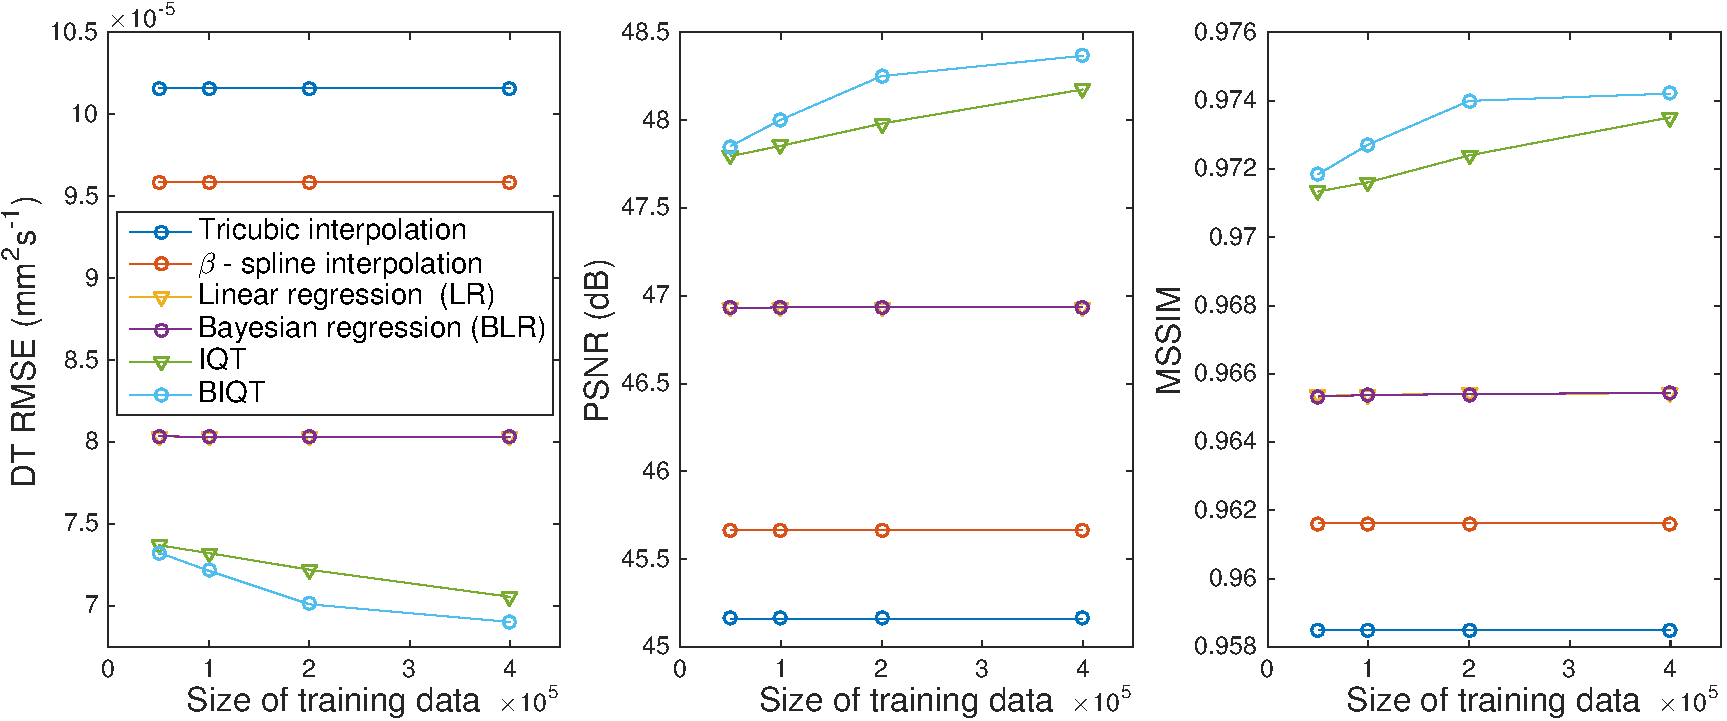
\includegraphics[width= \linewidth]{chapter_2/figure_3.pdf}
		\small 
		\caption{\small Three reconstruction metrics of various SR methods as a function of training data size; RMSE (left), PSNR (middle) and MSSIM (right). The performance of LR (yellow) and BLR (purple) coincide. The results for linear and nearest-neighbour interpolation are omitted for their poor performance.} 
		\label{fig:performance}
	\end{figure}

	Standard linear regression performs as well as the Bayesian regression due to the large training data size. However, with BIQT, as you descend each tree, the number of training data points at each node gets smaller, increasing the degree of uncertainty in model fitting, and so the data-driven regularisation performed in each node-wise Bayesian regression becomes more effective, leading to better reconstruction quality. This is also manifested in the deeper structure of BIQT trees, indicating more successful validation tests and thus greater generalisability. Moreover, BIQT performs reconstruction almost as efficiently as the original IQT, taking only a few minutes for full volume.
			
	\begin{figure}[ht]
		\begin{subfigure}{0.45\textwidth}
			\caption{Maximum Likelihood}
			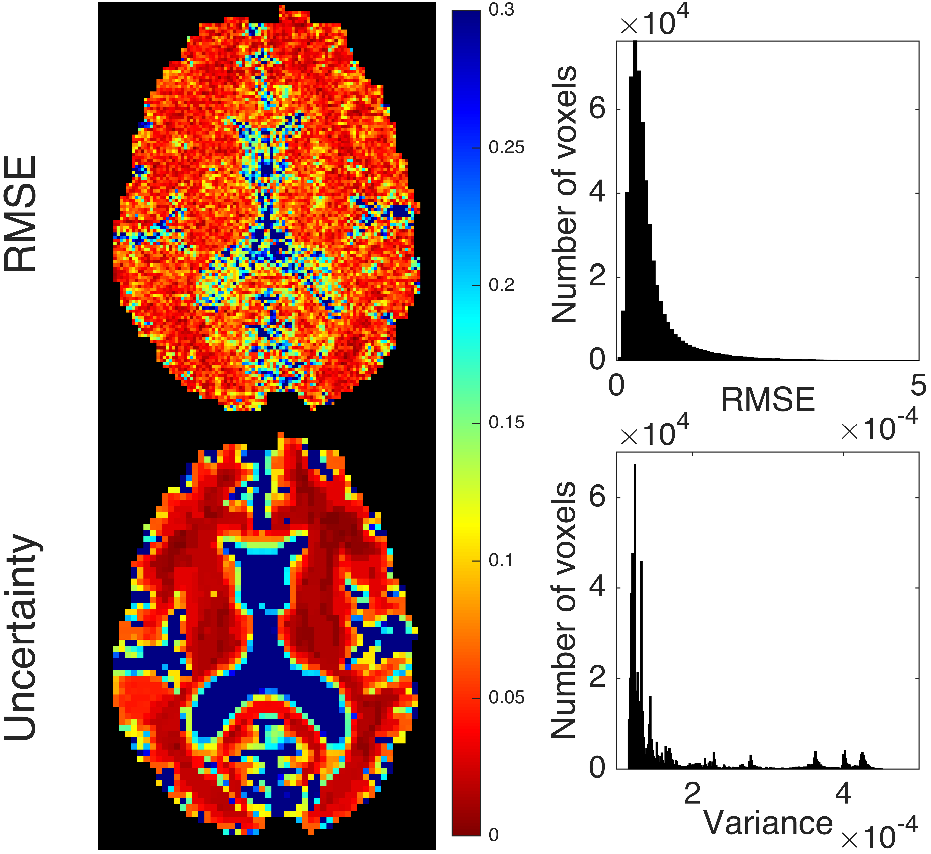
\includegraphics[width=8 cm]{chapter_2/figure_4.pdf}
			\label{fig:map1}
		\end{subfigure}
		\hfill
		\begin{subfigure}{0.43\textwidth}
			\caption{Locally Bayesian RF}
			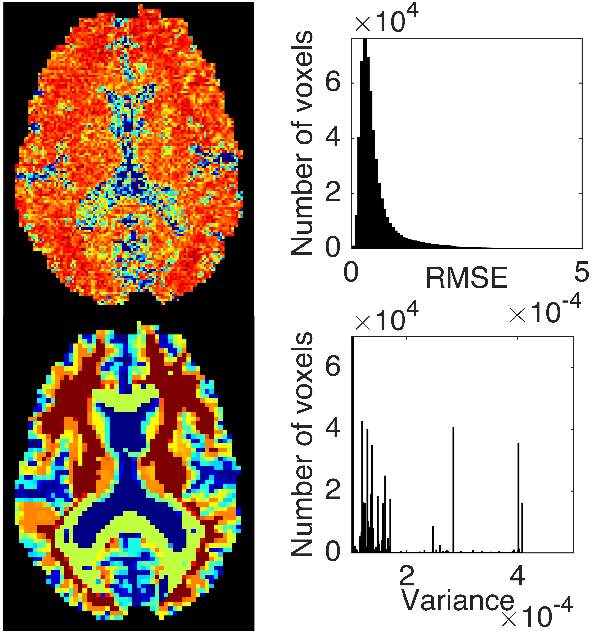
\includegraphics[width=6.9cm]{chapter_2/figure_5.pdf}
			\label{fig:map3}
		\end{subfigure}

%		\subfigure[Original IQT]{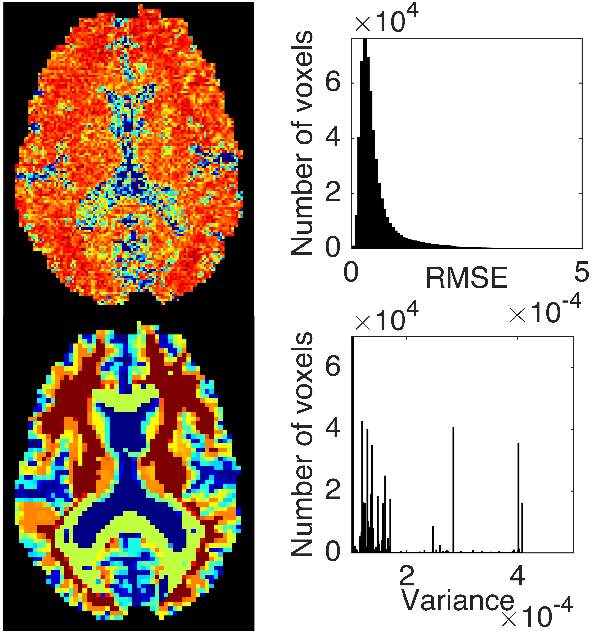
\includegraphics[width=6.9cm]{chapter_2/figure_5.pdf}\label{fig:map3}}
%		%\includegraphics[width=12.cm]{RMSEandConfidMAP_2.pdf}
		\small\caption[Optional caption for list of figures]{ 
			Reconstruction accuracy and uncertainty maps. (top row) The voxel-wise RMSE as a normalised colour-map and its distribution; (bottom row) Uncertainty map (variance) over the super-resolved voxels and its distribution for (a) BIQT and (b) IQT. Trees were trained on $\approx 4\times10^5$ patch pairs.} 
		\label{fig:confidencemap}
		%\vspace{- 10pt}
	\end{figure}

	
	Fig. \ref{fig:confidencemap} shows reconstruction accuracies and uncertainty maps for BIQT and IQT. The uncertainty map of BIQT is more consistent with its reconstruction accuracy when compared to the original IQT. Higher resemblance is also observed between the distribution of accuracy (RMSE) and uncertainty (variance). The BIQT uncertainty map also highlights subtle variations in the reconstruction-quality within the white matter, whereas the IQT map contains flatter contrasts with discrete uncertainties that vary greatly in the same region (see histograms in bottom row). This improvement reflects the positive effect of the data-driven regularisation and better generalisability of BIQT and can be observed particularly in the splenium and genu of the Corpus Callosum, where despite good reconstruction accuracy, IQT assigns higher uncertainty than in the rest of the white matter and BIQT indicates a lower and more consistent uncertainty. Thus, the BIQT uncertainty map displays higher correspondence with accuracy and allows for a more informative assessment of reconstruction quality. 
	%%%that the uncertainty map of BIQT (bottom row) is much more consistent with the reconstruction accuracy (top row) in comparison with that of original IQT. Higher resemblance is also observed between the distributions of accuracy (RMSE) and uncertainty (variance). The BIQT uncertainty map reflects some subtle variations in the reconstruction quality within white matter, whereas IQT simply assigns a fixed uncertainty to the whole region. Whilst IQT assigns high uncertainty to splenium and genu of Corpus Callosum despite high reconstruction accuracy, BIQT correctly indicates low uncertainty. The equivalent uncertainty measure for original IQT is solely determined by the training data and independent of the test input, which results in a discrete set of uncertainty values (fixed for each leave of a tree) as opposed to the continuous values attained by BIQT (compare the histograms in bottom row of figure \ref{fig:confidencemap}). 
	Note that while the uncertainty measure for IQT is governed purely by the training data, for BIQT the uncertainty also incorporates the familiarity of the test data.% (see figure \ref{fig:1D_uncertainty}). 
	
	\subsection{Testing on pathological brains}
	We further validate our method on images with previously unseen abnormalities; we use trees trained on healthy subjects from HCP dataset to super-resolve DTIs of MS and brain tumour patients (10 each). We process the raw data (DWI) as before, and only use $b = 1200 \text{ s/mm}^2$ measurements for the MS dataset and $b = 700 \text{ s/mm}^2$ for the tumour dataset. The voxel size for both datasets is $2^3 \text{ mm}^3$. The MS dataset also contains lesion masks manually outlined by a neurologist. Fig. \ref{fig:sickbrains}(a),(c) middle row shows that the uncertainty map of BIQT precisely identifies previously unseen features (pathologies in this case) by assigning lower confidence than for the remaining healthy white matter. Moreover, in accordance with the reconstruction accuracy, the prediction is more confident in pathological regions than in the cerebrospinal fluid (CSF). This is expected since the CSF is essentially free water with low SNR and is also affected by cardiac pulsations, whereas the pathological regions are contained within the white matter and produce better SNR. Each BIQT tree appropriately sends pathological patches into the `white-matter' subspace and its abnormality is detected there by the `familiarity' term, leading to a lower confidence with respect to the healthy white matter. By contrast, IQT sends pathological patches into the CSF subspace and assigns the fixed corresponding uncertainty which is higher than what it should be. In essence, BIQT enables an uncertainty measure which highly correlates with the pathologies in a much more plausible way, and this is achieved by its more effective partitioning of the input space and uncertainty estimation conferred by Bayesian inference. Moreover, Fig. \ref{fig:sickbrains}(b) shows the superior generalisability of BIQT even in reconstruction accuracy (here SR is performed on downsampled clinical DTIs); the RMSE of BIQT for MS patients is even smaller than that of IQT for healthy subjects. 


	\begin{figure}[ht]
		\centering
		\begin{subfigure}{0.50\linewidth}
			\caption{MS}
			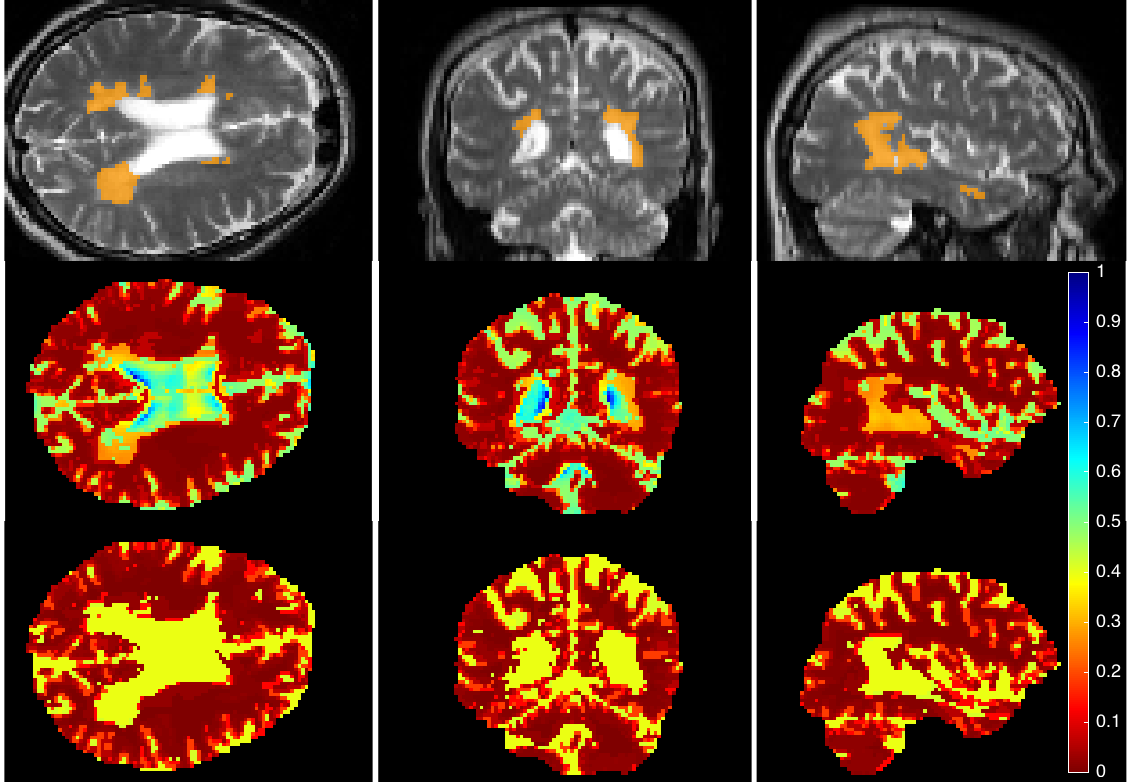
\includegraphics[width=\textwidth]{chapter_2/figure_6.png}
			\label{fig:map1}
		\end{subfigure}
		\begin{subfigure}{0.245\linewidth}
			\caption{RMSE}
			\includegraphics[width=\textwidth]{chapter_2/figure_7.pdf}
			\label{fig:map3}
		\end{subfigure}
   		\begin{subfigure}{0.23\linewidth}
    		\caption{Edema}
    		\includegraphics[width=\textwidth]{chapter_2/figure_8.png}
    		\label{fig:map2}
    	\end{subfigure}
%		\subfigure[MS]\label{fig:map1}}
%		\subfigure[RMSE]{\includegraphics[width=3.7cm]{figure_7.pdf}\label{fig:map3}}
%		\subfigure[Edema]{\includegraphics[width=3.55cm]{figure_8.png}\label{fig:map2}}
		\caption[Optional caption for list of figures]{(a),(c) Normalised uncertainty map (variance is shown i.e. the smaller the more certain) for BIQT (middle row) and IQT (bottom row) along with the T2-weighted slices (top row) for MS (with focal lesions in orange) and edema (contours highlighted), respectively. (b). The RMSE for MS and control subjects (averaged over $10$ subjects in each case).}
		\label{fig:sickbrains}
		%\vspace{-15pt}
	\end{figure}
		
	\section{Summary}
	We presented a computationally viable Bayesian extension of Image Quality Transfer (IQT). The application in super resolution of DTI demonstrated that the method not only achieves better reconstruction accuracy even in the presence of pathology (Fig. \ref{fig:map3}) than the original IQT and standard interpolation techniques, but also provides an uncertainty measure which is highly correlated with the reconstruction quality. Furthermore, the uncertainty map is shown to highlight focal pathologies not observed in the training data. BIQT also performs a computationally efficient reconstruction. Although we have only applied BIQT to DTI-SR, the method preserves the generality of IQT and future work will investigate its performance on tractography and parameter mapping applications. Also, diagnostic values of the method need to be validated in larger-scale experiments.
	
%
%
 
 %\documentclass[12pt]{article}
%\usepackage{geometry}
%\geometry{
%	a4paper,
%	total={170mm,257mm},
%	left=20mm,
%	top=20mm,
%}
%\usepackage{cite}
%\usepackage{hyperref}
%% *** GRAPHICS RELATED PACKAGES ***
%\usepackage{amsmath}
%\usepackage{amssymb}
%\usepackage{graphicx}
%\usepackage[FIGTOPCAP]{subfigure}
%\usepackage{wrapfig}
%\usepackage{soul}
%%\usepackage[subtle, title=normal, bibliography=normal]{savetrees24}
%
%\usepackage{bbm}
%\usepackage{caption}
%%\usepackage{subcaption}
%%\usepackage[bookmarks=false]{hyperref}
%
%%\captionsetup[figure]{belowskip=-50pt}
%%\usepackage{subcaption}
%%\usepackage{caption,subcaption}
%\usepackage[T1]{fontenc}
%\usepackage{capt-of}
%\usepackage[font=small,labelfont=bf,tableposition=top]{caption}
%\DeclareCaptionLabelFormat{andtable}{#1~#2  \&  \tablename~\thetable}
%
%\usepackage{floatrow}
%\floatsetup[figure]{font=footnotesize}
%\usepackage[T1]{fontenc}
%\usepackage[utf8]{inputenc}
%%\usepackage{babel}
%\usepackage[font=small,labelfont=bf]{caption}
%\newfloatcommand{capbtabbox}{table}[][\FBwidth]
%\usepackage[table]{xcolor}
%%\usepackage{floatrow}
%% Table float box with bottom caption, box width adjusted to content
%%\newfloatcommand{capbtabbox}{table}[][\FBwidth]
%
%\usepackage{graphics}
%
%\usepackage[amssymb]{SIunits}
%\usepackage{stackengine}
%\def\delequal{\mathrel{\stackon[1pt]{=}{$\scriptscriptstyle\Delta$}}}
%\usepackage{array}
%
%


\chapter{Predictive Uncertainty in Deep Learning}
\label{chapter:deepuncertainty}


%------------------ Abstract ------------------------------------
	Deep learning (DL) has shown great potential in medical image enhancement problems, such as super-resolution or image synthesis. However, to date little consideration has been given to uncertainty quantification over the output image. Here we introduce methods to characterise different components of uncertainty in such problems and demonstrate the ideas using diffusion MRI super-resolution.  Specifically, we propose to account for \textit{intrinsic uncertainty} through a heteroscedastic noise model and for \textit{parameter uncertainty} through approximate Bayesian inference, and integrate the two to quantify \textit{predictive uncertainty} over the output image. Moreover, we introduce a method to propagate the predictive uncertainty on a multi-channelled image to derived scalar parameters, and separately quantify the effects of intrinsic and parameter uncertainty therein. The methods are evaluated for super-resolution of two different signal representations of diffusion MR images---Diffusion Tensor images and Mean Apparent Propagator MRI---and their derived quantities such as mean diffusivity and fractional anisotropy, on multiple datasets of both healthy and pathological human brains. Results highlight three key potential benefits of uncertainty modelling for improving the safety of DL-based image enhancement systems. Firstly, incorporating uncertainty modelling improves the predictive performance even when test data departs from training data. Secondly, the predictive uncertainty highly correlates with reconstruction errors, and is therefore capable of detecting predictive ``failures''. Results on both healthy subjects and patients with brain glioma or multiple sclerosis demonstrate that such an uncertainty measure enables subject-specific and voxel-wise risk assessment of the super-resolved images that can be accounted for in subsequent analysis. Thirdly, we show that the method for decomposing predictive uncertainty into its independent sources provides high-level ``explanations'' for the model performance by separately quantifying how much uncertainty arises from the inherent difficulty of the task or the limited training examples. The introduced concepts of uncertainty modelling extend naturally to many other imaging modalities and data enhancement applications.


%------------------------------------ Introduction  ------------------------------
\section{Introduction}
% (Interesting to motivate)
%The most widely used deep learning models have an important shortcoming: they lack an under- lying mechanism to provide uncertainty infor- mation about the predictions they make. Instead they often output point estimates between 0 and 1, which are often taken blindly as a measure of confidence. There have already been a few high profile cases where blindly trusting deci- sions made by deep learning algorithms has had disastrous consequences. For example in 2016, and then again in 2018, there were fatalities due to mistakes made by the perception system of autonomous vehicles. In health care a wrong decision can be a matter of life or death, and so being able to place trust in the decisions of deep learning models applied to such an industry is of critical importance.

In the last few years, deep learning techniques have permeated the field of medical image processing \cite{shen2017deep,litjens2017survey}. Beyond the automation of existing radiological tasks--- e.g. segmentation \cite{kamnitsas2017efficient}, detection \cite{roth2014new}, disease grading and classification \cite{araujo2017classification}---deep learning has been applied to a diverse set of ``data enhancement'' problems. Data enhancement aims to improve the quality, the information content, or the quantity of medical images available for research and clinics by transforming images from one domain to another \cite{isola2017image}. Previous research has shown the efficacy of data enhancement in different forms such as super-resolution \cite{oktay2016multi,chen2018efficient,ravi2019adversarial}, image synthesis \cite{nie2016estimating,kang2017deep}, denoising \cite{benou2017ensemble,chen2017low}, data harmonisation \cite{karayumak2018harmonizing,tax2019cross} across scanners and protocols, reconstruction \cite{sun2016deep,jin2017deep,hammernik2018learning,schlemper2018deep,zhu2018image,yang2018dagan,yoon2019efficient}, registration \cite{sokooti2017nonrigid,balakrishnan2018unsupervised} and quality control \cite{wu2017fuiqa,esses2018automated}.  These advances have the potential not only to enhance the quality and efficiency of radiological care, but also facilitate scientific discoveries in medical research through increased volume and content of usable data. 

However,  most efforts in the development of data enhancement techniques have focused on improving the accuracy of deep learning algorithms, with little consideration of risk management. Blindly trusting the output of a given machine learning tool risks undetected failures e.g. spurious features and removal of structures \cite{cohen2018distribution}. In medical applications, images inform scientific conclusions in research, and diagnostic, prognostic and interventional decisions in clinics. Therefore, translation of current proofs of principle to such safety-critical applications demands mechanisms for quantifying the risks of failures i.e. quantification of uncertainty/confidence and explanation of its source \cite{begoli2019need}. 

\begin{figure}[t]
	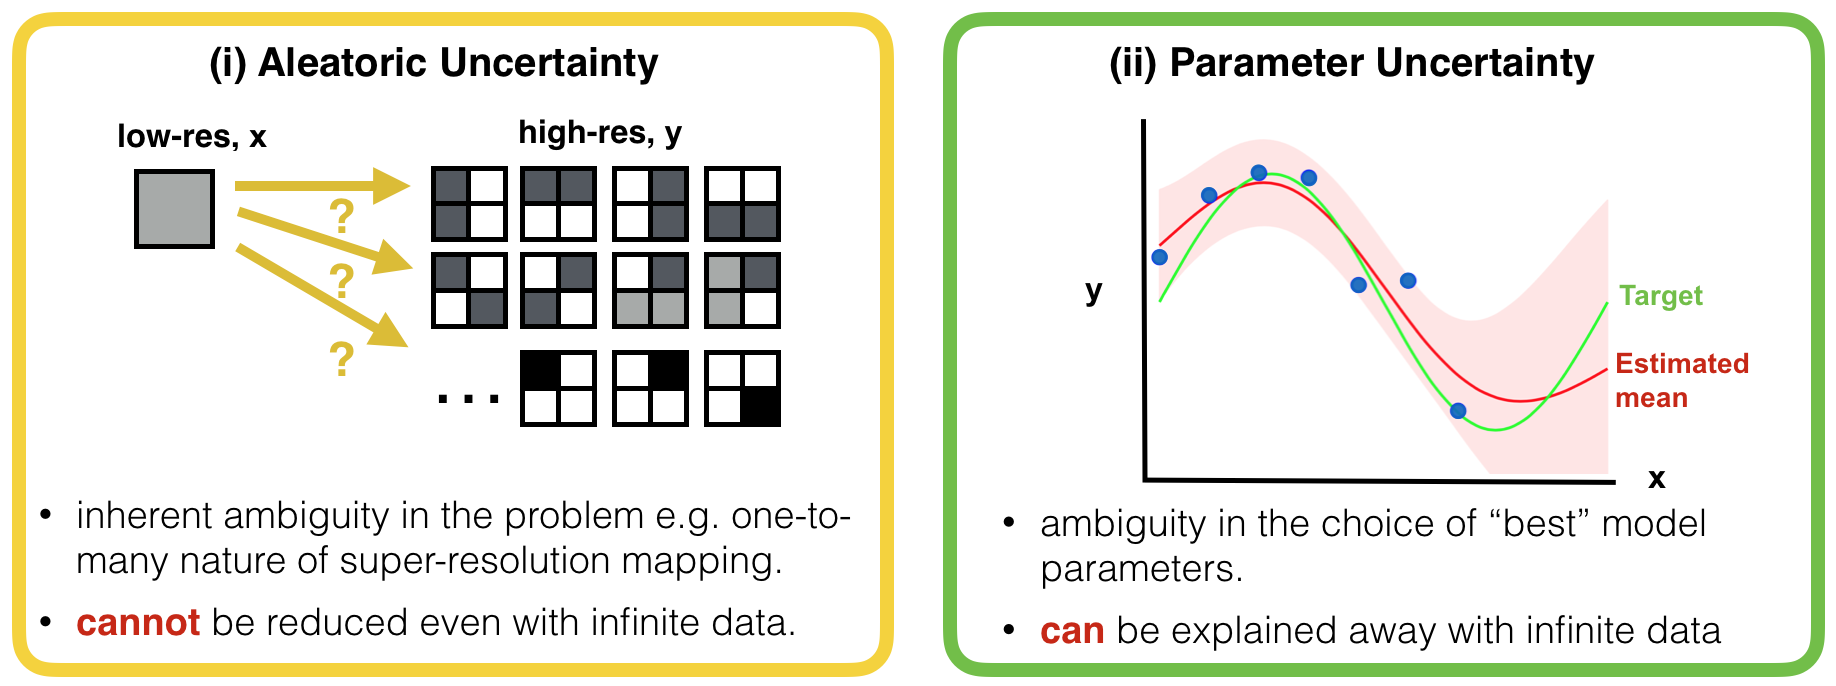
\includegraphics[width=0.95\linewidth]{chapter_3/figures/fig_intro.png}
	\centering	
%	\vspace{-2mm}
	\caption{Illustration of two different types of uncertainty \cite{hora1996aleatory}. Intrinsic uncertainty \cite{wang1996intrinsic} quantifies the degree of inherent ambiguity in the underlying problem. For example, in the case of super-resolution, there exist many possible high-resolution images $\textbf{y}$ that would get mapped onto the same low-resolution input $\textbf{x}$. Intrinsic uncertainty is irreducible with training data. On the other hand, the parameter uncertainty \cite{draper1995assessment} (a subtype of model uncertainty) arises from the finite training set. There exist more than one model that can explain the given training data equally well, and the parameter uncertainty quantifies the ambiguity in selecting the model parameters that best captures the target data-generating process. As illustrated in the figure on the right, parameter uncertainty decreases with more data; the green line shows the target function, the red line is the estimated mean, and the shaded region signifies the associated parameter uncertainty (standard deviation), which is higher in regions where we have fewer observations.} 
	\label{fig:uncertainty_types}
	%\vspace{-10pt}
\end{figure}

Predictive failures of deep learning systems, by and large, occur due to two reasons: i) the task itself is inherently ambiguous or ii) the learned model is not adequate to describe the data  \cite{hora1996aleatory,der2009aleatory,tanno2017bayesian,kendall2017uncertainties}, as illustrated in Fig.~\ref{fig:uncertainty_types}. The former stems from \emph{intrinsic uncertainty} \cite{wang1996intrinsic}, which describes ambiguity in the underlying data generating process  (e.g. presence of stochasticity such as measurement noise and intrinsic ill-posed nature of the problem), and cannot be alleviated by increasing available training data or model complexity\footnote{Intrinsic uncertainty is also known as \textit{aleaotoric} or statistical uncertainty.}. The latter is characterised by \textit{model uncertainty}\cite{draper1995assessment}, which describes ambiguity in model specification\footnote{Model uncertainty is a subclass of \textit{epistemic uncertainty} \cite{hora1996aleatory} which encompasses types of uncertainties that arise from lack of knowledge. }. Model uncertainty arises from a) \textit{parameter uncertainty}: ambiguity in fitting the model to the target mapping due to limited training data, or b) \textit{model bias}: errors due to insufficient flexibility of the model class (e.g. fitting a linear model to a sinusoidal process). These types of uncertainty can be reduced by collecting more data or specifying a different class of models. With the expressivity of deep neural networks, which are known to be universal approximators \cite{cybenko1989approximation} if sufficiently large, one might reasonably assume that the model bias is small enough to be discounted. Under this assumption, intrinsic and parameter uncertainty (Fig.~\ref{fig:uncertainty_types}) fully characterise the predictive failures of deep learning models. Therefore, accurate estimation of these uncertainties are needed and would potentially allow practioners to understand better the limits of the models, flag doubtful predictions, and highlight test cases that are not well represented in the training data.

%Fig.~\ref{fig:uncertainty_types} illustrates the differences between intrinsic and parameter uncertainty, the two key types of uncertainty that need to be considered to characterise the limits of deep learning models. 

% (Ryu): I think we should mention the previous work... 
%Kiureghian \emph{et al.}  \cite{der2009aleatory} first proposed such categorisation of uncertainty in statistical modelling, and adovocated its importance in the assessment of structural safety e.g. seismic collapse risk of buildings.  More recently, Tanno \emph{et al.}  \cite{tanno2017bayesian} extended this argment to deep learning systems and demonstarated the importance of modelling both intrinsic and parameter uncertainty to build more robust predictive models for medical imaging. Kendall \emph{et al.} \cite{kendall2017uncertainties} concurrently investigated the same problem in computer vision, suggesting its utility for safety-critical applications such as self-driving cars. 

%\textcolor{red}{What is unique about medical applications that puts particular demands on uncertainty quantification - is it different in any way to the challenge in computer vision?}

In this work, we introduce methods for capturing components of uncertainty in medical image enhancement systems based on deep learning. We propose to model intrinsic uncertainty through a input-dependent (heteroscedastic) noise model \cite{nix1994estimating} and parameter uncertainty through variational dropout \cite{kingma2015variational}. We then combine and propagate these two ``source'' uncertainties into a spatial map of \textit{predictive uncertainty} over the output image, which can be used to assess the output reliability on subject-specific and voxel-wise basis. Lastly, we propose a method to propagate the predictive uncertainty to arbitrary derived quantities of the output images, such as scalar indices that are commonly used for subsequent analysis, and decompose it into distinct components which separately quantify the contributions of intrinsic and parameter uncertainty. This paper demonstrates the benefits of these ideas to enhancing system safety within the context of Image Quality Transfer (IQT) \cite{alexander2014image,tanno2016bayesian,alexander2017image,blumberg2018deeper}, a data-enhancement framework for propagating information from rare or expensive high quality images to lower quality but more readily available images. We focus on the application of IQT to \textit{super-resolution} of diffusion magnetic resonance imaging (dMRI) scans, and evaluate the utility of uncertainty quantification in terms of three aspects; i) performance on unseen datasets; ii) safety assessment of system output; iii) explainability of failures. For two different types of diffusion signal representations, we evaluate the effects of uncertainty modeling on generalisation by measuring the predictive accuracy on unseen test subjects in the Human Connectome Project (HCP) dataset \cite{sotiropoulos2013advances} and the Lifespan dataset \cite{harms2018extending}. We additionally test the value of improved predictive performance in a downstream tractography application. We then test the capability of the predictive uncertainty map to indicate predictive errors and thus to detect potential failures on images of both healthy subjects and those in which pathologies unseen in the training data arise, specifically from glioma and multiple-sclerosis (MS) patients. Lastly, we perform the decomposition of predictive uncertainty on HCP subjects with benign abnormalities, and assess its potential value in gaining high-level interpretations of predictive performance. 


\section{Related Works}
This section provides a review of related works under several different themes. We first review the development of learning-based image enhancement methods in medical imaging applications. We then discuss the recent advances made to model and quantify uncertainty in such image enhancement problems. Lastly, we describe the existing strands of research in uncertainty modelling for other medical imaging problems and fields of applications. 

Various forms of image enhancement can be cast as image transformation problems where the input image from one domain is mapped to an output image from another domain. Numerous recent methods have proposed to perform image transformation tasks as supervised regression of low quality against high quality image content. Alexander \emph{et al.} \cite{alexander2014image} proposed Image Quality Transfer (IQT), a general framework for supervised quality enhancement of medical images. They demonstrated the efficacy of their method through a random forest (RF) implementation of super-resolution (SR) of brain diffusion tensor images and estimation of advanced microstructure parameter maps from sparse measurements. More recently, deep learning, typically in the form of convolutional neural networks (CNNs), has shown additional promise in this kind of task. For example, Oktay \emph{et al.} \cite{oktay2016multi} proposed a CNN model to upsample a stack of 2D MRI cardiac volumes in the through-plane direction, where the SR mapping is learnt from 3D cardiac volumes of nearly isotropic voxels. This work was later extended by \cite{oktay2018anatomically} with the addition of global anatomical prior based on auto-encoder. Zhao \emph{et al.} \cite{zhao2018deep} proposed a solution to the same SR problem for brains that utilises the high frequency information in in-plane slices to super-resolve in the through-plane direction without requiring external training data. In addition, a range of different architectures of CNNs have been considered for SR of other modalities and anatomical structures such as structural MRI \cite{chen2018efficient} of brains, retinal fundus images \cite{mahapatra2017image} and computer tomography (CT) scans of chest \cite{yu2017computed}. Another problem of growing interest is image synthesis, which aims to synthesise an image of a different modality given the input image. Nie \emph{et al.} \cite{nie2018medical} employed a conditional generative adversarial network to synthesise CT from MRI with fine texture details whilst Wolterink \emph{et al.} \cite{wolterink2017deep} extended this idea using a CycleGAN \cite{zhu2017unpaired} to leverage the abundance of unpaired training sets of CT and MR scans. In \cite{bahrami2016convolutional}, a variant of CNN  was applied to predict 7T images from 3T MRI, where both contrast and resolution are enhanced. Another notable application is the harmonisation of diffusion MRIs \cite{karayumak2018harmonizing,tax2019cross,blumberg2018deeper,blumberg2019msp} where images acquired at different scanners or magnetic field strengths are mapped to the common reference image space to allow for joint analysis.  

Despite this advancement, all of these methods commit to a single prediction and lack a mechanism to communicate uncertainty in the output image.  In medical applications where images can ultimately inform life-and-death decisions, quantifying reliability of output is crucial. Tanno \emph{et al.} \cite{tanno2016bayesian} aimed to address this problem for supervised image enhancement for the first time by proposing a Bayesian variant of random forests to quantify uncertainty over predicted high-resolution MRI. They showed that the uncertainty measure correlates well with the accuracy and can highlight abnormality not represented in the training data. In our preliminary work \cite{tanno2017bayesian}, we made an initial attempt
to extend this approach with probabilistic deep-learning formulation, and showed that modelling different components of uncertainty---intrinsic and parameter uncertainty---allows one to build a more generalisable model and quantify predictive confidence. Kendall \emph{et al.} \cite{kendall2017uncertainties} concurrently investigated the same problem in computer vision, suggesting its utility for safety-critical applications such as self-driving cars. More recently, Hu \emph{et al.}\cite{hu2019uncertainty} extended these works in the context of medical image segmentation and proposed a mechanism to learn the intrinsic uncertainty in a supervised manner, when multiple labels are available. Dalca \emph{et al.} \cite{dalca2018unsupervised} proposed a CNN-based probabilistic model for diffeomorphic image registration with a learning algorithm based on variational inference, and demonstrated the state-of-the-art registration accuracy on established benchmarks while providing estimates of registration uncertainty. An alternative approach is ensembling where the variance of the predictions of multiple networks is used to quantify the predictive uncertainty \cite{lakshminarayanan2017simple}. Schlemper \emph{et al.} \cite{schlemper2018stochastic} proposed a novel combination of the cascaded CNN architecture and compressive sensing, equipped with a variant of ensemble techniques, which enabled robust reconstruction of highly undersampled cardiovascular diffusion MR images, and quantification of reconstruction uncertainty. Bragman \emph{et al.} \cite{bragman2018uncertainty} studied the value of uncertainty modelling for multi-task learning in the context of MR-only radiotherapy treatment planning where the synthetic CT image and the segmentation of organs at risk are simultaneously predicted from the input MRI image.  

We should also note that, although not the focus of this work, research on uncertainty modelling in deep learning techniques extend to other medical image processing tasks beyond data enhancement, such as segmentation, detection and classification. For example, Nair \emph{et al.}, \cite{nair2018exploring} demonstrated for lesion segmentation of multiple sclerosis that the voxel-wise uncertainty metrics can be used for quality control; by filtering out predictions with high uncertainty, the model could achieve higher lesion detection accuracy. A concurrent work by Eaton-Rosen \emph{et al.} \cite{eaton2018towards} showed for the task of brain tumour segmentation that the Monte Carlo (MC) sample variance from dropout \cite{gal2015dropout} can be calibrated to provide meaningful error bars over estimates of tumour volumes. Similarly,  \cite{roy2019bayesian} introduced ways to turn voxel-wise uncertainty score into structure-wise uncertainty metrics for brain parcellation task, and showed their values in performing more reliable group analysis. The uncertainty metric based on MC dropout has also shown promise in disease grading of retinal fundal images \cite{worrall2016automated,leibig2017leveraging}, and more recently an extension based on test-time augmentation was introduced by \cite{ayhan2018test}. An alternative approach is to train a model to predict uncertainty score directly; \cite{Raghu2018DirectUP} showed that this approach is more effective when opinions from multiple experts are available for each image. Koh \emph{et al.} \cite{kohl2018probabilistic} and Baumgartner \emph{et al.} \cite{PHiSeg2019Baumgartner} proposed methods to generate a set of diverse and plausible segmentation proposals on a given image, capturing more realistically the high inter-reader annotation variability, which is commonly observed in medical image segmentation tasks. Lastly, \cite{raykar2010learning,tanno2019learning} demonstrated for the classification of mammograms and cardiac ultra-sound images, respectively that modelling uncertainty and biases of individual annotators enables robust learning from noisy labels in the presence of large disagreement. 

However, within the context of medical image enhancement, these lines of research performed only limited validation of the quality and utility of uncertainty modelling. In this work, we formalise and extend the preliminary ideas in Tanno \emph{et al.} \cite{tanno2017bayesian} and provide a comprehensive set of experiments to evaluate the proposed uncertainty modelling techniques in a diverse set of datasets, which vary in demographics, scanner types, acquisition protocols or pathology. Moreover, with the exception of \cite{tanno2017bayesian}, none of the previous methods model different components of uncertainty, namely intrinsic and parameter uncertainty. Our method accounts for both, and provides conclusive evidence that this improves performance thanks to different regularisation effects. In addition, we propose a method to decompose predictive uncertainty over an arbitrary function of the output image (e.g. morphological measurements) into its sources, in order to provide a high-level explanation of model performance on the given input. 


\subsection{Modern Probabilistic Deep Leaning}
\textcolor{red}{This section will review theoretical research on uncertainty modelling in deep learning. We will discuss why such research is important for designing safe and interpretable systems for medical applications. } 

\textcolor{red}{This thesis is a mixture of applications of these methods to practical medical imaging problems, and development of new methods building upon such work. }



% Previous version (2-19-04-24): 
%However, despite this advancement, all of these methods commit to a single prediction and lack a mechanism to communicate uncertainty in the output image.  In medical applications where images can ultimately inform life-and-death decisions, quantifying reliability of prediction is particularly important. Tanno \emph{et al.} \cite{tanno2016bayesian} made the initial attempt to consider this problem for supervised image enhancement; a Bayesian variant of random forests was designed to provide an estimate of uncertainty over predicted high-resolution MRI. They showed that the predictive uncertainly correlates well with the accuracy and can highlight abnormality not represented in the training data. \cite{tanno2017bayesian} extended this approach with probabilistic deep-learning formulation, in which \textit{intrinsic uncertainty} is estimated through a per-patch heteroscedastic noise model and \textit{parameter uncertainty} is modelled through approximate Bayesian inference. In particular, it was shown that modelling different components of uncertainty allows one to build a more generalisable model and quantify predictive confidence. Dalca \emph{et al.} \cite{dalca2018unsupervised} proposed a CNN-based probabilistic model for diffeomorphic image registration with a learning algorithm based on variational inference, and demonstrated the state of the art registration accuracy on established benchmarks while providing estimates of registration uncertainty. An alternative promising approach is ensembling where the variance of the predictions of multiple networks is used to quantify the predictive uncertainty \cite{lakshminarayanan2017simple}; the novel combination of the cascaded CNN architecture and compressive sensing, endowed with a variant of ensemble techniques \cite{schlemper2018stochastic}, enabled robust reconstruction of highly undersampled diffusion tensor cardiovascular MR, and quantification of reconstruction uncertainty that shows high correspondence with the errors. Bragman \emph{et al.} \cite{bragman2018uncertainty} studied the value of uncertainty modelling for multi-task learning in the context of MR-only radiotherapy treatment planning where the synthetic CT image and the segmentation of organs at risk are simulatenously predicted from the input MR image. By explicitly modelling input-dependent noise in the predictions, they derived a learning algorithm that naturally weights task specific losses on a per-example basis, which improves the predictive performance and yields well-calibrated uncertainty estimates. In this paper, building upon the prior work  \cite{tanno2017bayesian}, we evaluate extensively on the datasets of healthy and diseased brains the utility of estimated predicted uncertainty in safeguading against failures in MR supre-solution task and additionally propose a method to decompose such uncertainty measure into factors of variations for increased explainability. 




%\begin{itemize}
%%	\item Segmentation: Zach's paper \cite{eaton2018towards}, Tanya's paper \cite{nair2018exploring}
%	\item classification: Leibig \cite{leibig2017leveraging}, Test-time augmentation for retina fundas image classification \cite{ayhan2018test}, Ehigh-res time-series prediction \cite{heo2018uncertainty}
%	\item others: directly estimating uncertainty score in classification task \cite{Raghu2018DirectUP}.
%	\item Quality control of T1 segmentation: Wachinger \emph{et al.}, \cite{roy2019bayesian}
%\end{itemize}

%\textbf{Uncertainty categorization:} Kiureghian \emph{et al.}  \cite{der2009aleatory} first proposed such categorisation of uncertainty in statistical modelling, and adovocated its importance in the assessment of structural safety e.g. seismic collapse risk of buildings.  More recently, Tanno \emph{et al.}  \cite{tanno2017bayesian} extended this argment to deep learning systems and demonstarated the importance of modelling both intrinsic and parameter uncertainty to build more robust predictive models for medical imaging. Kendall \emph{et al.} \cite{kendall2017uncertainties} concurrently investigated the same problem in computer vision, suggesting its utility for safety-critical applications such as self-driving cars. 



%% May be useful for the thesis:
%
%Finally, talk more generally about uncertaint modelling with deep neural networks. 
%\begin{itemize}
%	\item importance of considering two different types of uncertainty in computer vision applications \cite{kendall2017uncertainties} 
%	\item  Summary of uncertainty modelling methods e.g. Bayesian NNs \cite{kingma2015variational,gal2015dropout,gal2017concrete}, ensemble \cite{lakshminarayanan2017simple}, MCMC methods. 
%	\item Other probabilistic models based on DNNs e.g. Density estimation (real-valued NVP  transoformation, GANs, heteroscedastic model, auto-regressive model).
%\end{itemize}
Not too sure how important to have a thorow review of these advancements, may be refer to a paper with a good review e.g. \cite{wu2018deterministic}? 



% ------------------- Methods/Theory -------------------
\section{Methods}
This section describes the methods for modelling different components of uncertainty that arise in data enhancement. Firstly, we provide an overview of Image Quality Transfer (IQT) which formulates data enhancement as a supervised learning problem. Secondly, using the IQT framework, we introduce methods to model \textit{intrinsic} and \textit{parameter uncertainty}, separately, focusing on the application of super-resolution. We then combine the two approaches and estimate the overall uncertainty over prediction (\textit{predictive uncertainty}) by approximating the variance of the predictive distribution (eq.~\eqref{eq:full_distribution}). Lastly, we propose a method for decomposing predictive uncertainty into its sources---intrinsic and parameter uncertainty---in an attempt to provide quantifiable explanations for the confidence on model output (eq.~(\ref{eq:variance_decomposition})). 


\subsection{Background: Image Quality Transfer}
Alexander \emph{et al.} \cite{alexander2014image} proposed Image Quality Transfer (IQT), the first supervised learning based framework for data enhancement of medical images, and here we survey its general formulation which forms the testing ground of this work. IQT performs data enhancement via regression of low quality against high quality image content. In order to overcome the memory demands of processing 3-dimensional medical images, along with other subsequent work such as \cite{yang2016fast,oktay2016multi,bahrami2016convolutional,oktay2018anatomically}, IQT assumes factorisability over local neighbourhoods (also called patches) and models the conditional distribution of high-quality image $I_{High}$ given the corresponding low-quality input $I_{Low}$ as: 
\begin{equation}
p(I_{High}|I_{Low}) = \prod_{i\in \mathcal{S}} p(\mathbf{y}_{i}|\mathbf{x}_{i})
\end{equation}
where $\{\textbf{y}_{i}\}_{i \in \mathcal{S}}$ is a set of disjoint high-quality subvolumes with $\mathcal{S}$ denoting the set of their indices, which together constitute the whole image $I_{High}$, while $\{\textbf{x}_{i}\}_{i \in \mathcal{S}}$ is a set of potentially overlapping low-quality subvolumes, each of which contains and is spatially larger than the corresponding $\textbf{y}_{i}$, as illustrated in Fig.~\ref{fig:iqt_illustration}. Here we assume that each local neighbourhood is a cubic sub-volume. The locality assumption reduces the problem of learning $p(I_{High}|I_{Low})$ to the much less memory intensive problem of learning $p(\mathbf{y}|\mathbf{x})$. In other words, IQT formulates the data enhancement task as a patch-wise regression where an input low-quality image $I_{Low}$ is split into smaller overlapping sub-volumes  $\{\textbf{x}_{i}\}_{i \in \mathcal{S}}$ and the corresponding non-overlapping high-quality sub-volumes $\{\textbf{y}_{i}\}_{i \in \mathcal{S}}$ are independently predicted according to the patch regressor $p(\mathbf{y}|\mathbf{x})$. The final prediction for the 3D high-quality volume $I_{high}$ is constructed by tesellating the output patches $\{\textbf{y}_{i}\}_{i \in \mathcal{S}}$. 

\begin{figure}[t]
	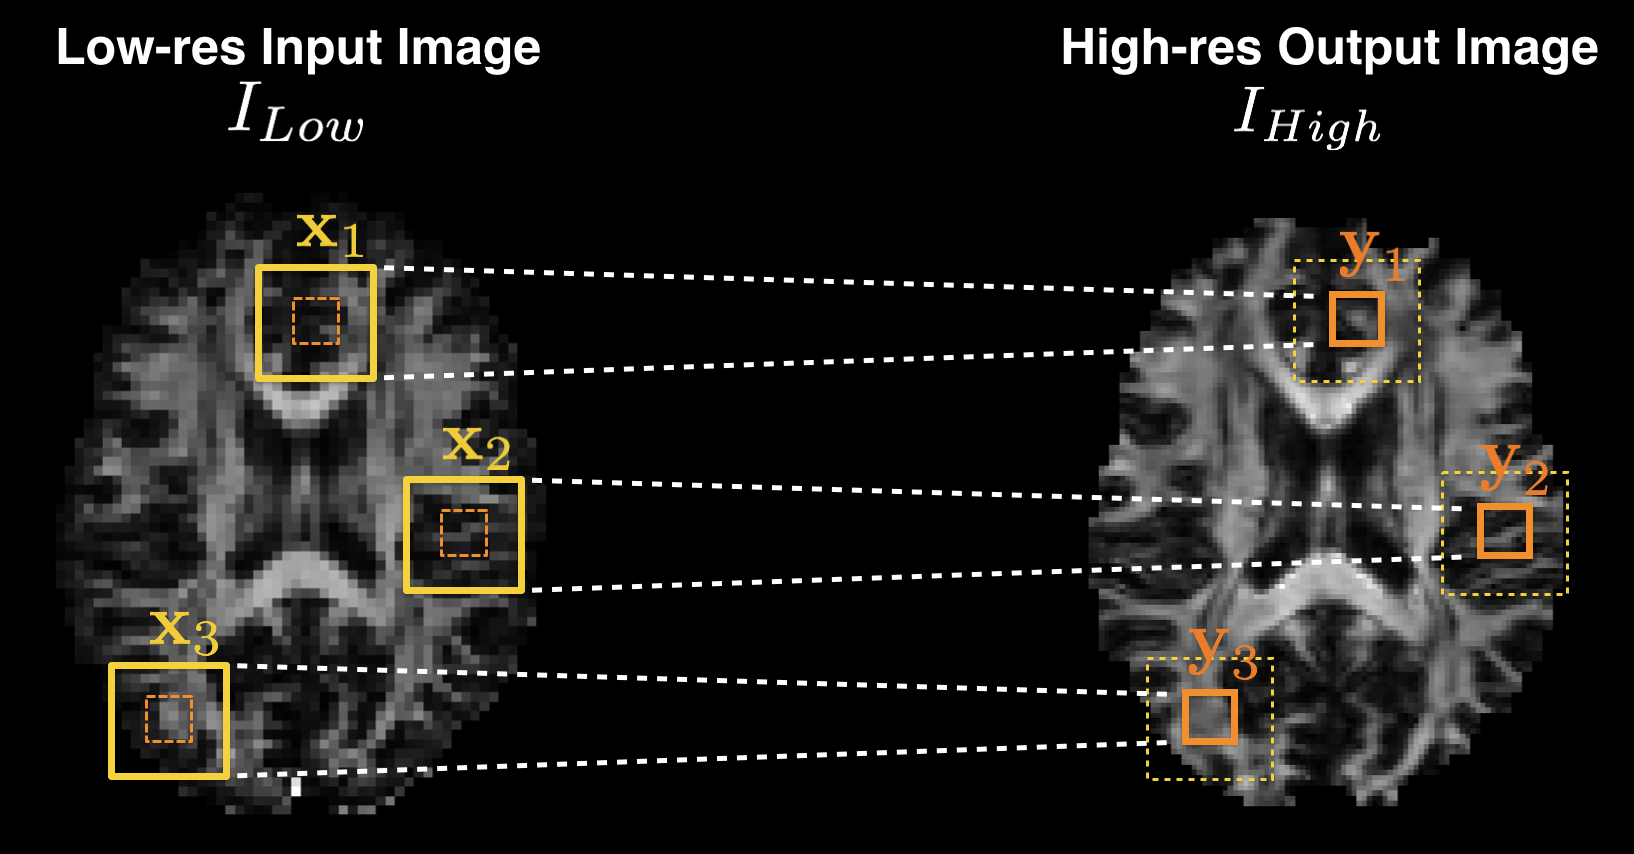
\includegraphics[width=0.8\linewidth]{chapter_3/figures/iqt_illustration.png}
	\centering	

	\caption{Illustration of the patch-wise regression in super-resolution application. The conditional distribution over the high quality image $p(I_{High}|I_{Low})$ is assumed to factorise over local neighbourhoods $\{(\mathbf{x}_i, \mathbf{y}_i)\}_{i}$. In this case, for each input subvolume $\mathbf{x}_{i}$ (in yellow), the high resolution version of the smaller centrally located neighbourhood, $\mathbf{y}_{i}$ (in orange) is regressed. } 
	\label{fig:iqt_illustration}
	
	%\vspace{-10pt}
\end{figure}

The original implementation of IQT \cite{alexander2014image,alexander2017image,tanno2016bayesian} employed a variant of random forests (RFs) to model $p(\mathbf{y}|\mathbf{x})$ while more recent \cite{yang2016fast,oktay2016multi,bahrami2016convolutional,oktay2018anatomically} approaches use variants of convolutional neural networks (CNNs). Either way, the machine learning algorithm is trained on pairs of high-quality and low-quality patches $\mathcal{D}=\{(\mathbf{x}_i,\mathbf{y}_i)\}_{i=1}^N$ extracted from a set of image volumes, and is used to perform the data-enhancement task of interest.  Typically, such patch pairs $\mathcal{D}$ are synthesised by down-sampling a collection of high quality images to approximate their counterparts in a particular low-quality scenario \cite{alexander2014image,oktay2016multi}. In this work, we focus on the task of super-resolution (SR) where the spatial resolution of $I_{high}$ is higher than the input image $I_{low}$. 

\subsection{Baseline Super-Resolution Model: 3D-ESPCN} \label{sec:baseline}
As the baseline architecture for modelling $p(\mathbf{y}|\mathbf{x})$, we adapt efficient subpixel-shifted convolutional network (ESPCN) \cite{shi2016real} to 3D data. ESPCN is a recently proposed method with the capacity to perform real-time per-frame SR of videos while retaining high accuracy on 2D natural images.  We have chosen to base on this architecture for its simplicity and computational performance. Most CNN-based SR techniques first up-sample a low-resolution input image (e.g. through bilinear interpolation\cite{dong2016image}, deconvolution\cite{oktay2016multi,mcdonagh2017context}, fractional-strided convolution\cite{johnson2016perceptual}, etc) and then refine the high-resolution estimate through a series of convolutions. These methods suffer from the fact that $(1)$ the up-sampling can be a lossy process and $(2)$ refinement in the high-resolution space has a higher computational cost than in the low-resolution space. By contrast, ESPCN performs convolutions in the low-resolution-space, upsampling afterwards. The reduced resolution of feature maps dramatically decreases the computational and memory costs, which is more pronounced in processing 3D data.

More specifically the ESPCN is a fully convolutional network, with a special \emph{shuffling operation} on the output, which identifies individual feature channel dimensions with spatial locations in the high-resolution output. Fig.~\ref{fig:ESPCN} shows a 2D illustration of an example ESPCN when the fully convolutional part of the network consists of 3 convolutional layers, each followed by a ReLU, and the final layer has $cr^2$ feature maps where $r$ is the upsampling rate and $c$ is the number of channels in the output image (e.g. $6$ in the case of DT images). The shuffling operation takes the feature maps of shape $h\times w\times cr^2$ and remaps pixels from different channels into different spatial locations in the high-resolution output, producing a $rh\times rw\times c$ image, where $h$ and $w$ denote height and width of the pre-shuffling feature maps. This shuffling operation in 3D is given by $\mathcal{S}(F)_{i,j,k,c} =  F_{[i/r],[j/r],[k/r],(r^3-1)c + \text{mod}(i,r) + r\cdot \text{mod}(j,r) + r^3\cdot \text{mod}(k,r)}$ where $F$ is the pre-shuffled feature maps. The combined effects of the last convolution and shuffling is effectively a learned interpolation, and an efficient implementation of deconvolution layer \cite{zeiler2011adaptive} where the kernel size is divisible by the size of the stride \cite{shi2016real}. Therefore, it is less susceptible to checker-board like artifacts commonly observed with deconvolution operations \cite{odena2016deconvolution}.


At test time, the prediction of higher resolution volume is performed through \textit{shift-and-stitch} operation. The network takes each subvolume $\mathbf{x}$ in a low-resolution image, and predicts the corresponding high-resolution sub-volume $\mathbf{y}$. By tessellating the predictions from appropriately shifted inputs $\mathbf{x}$, the whole high-resolution volume is reconstructed. With convolutions being local operations, each output voxel is only inferred from a local region in the input volume, and the spatial extent of this local connectivity is referred to as the \textit{receptive field}. For a given input subvolume, the network increases the resolution of the central voxel of each receptive field e.g. the central $2^3$ output voxels are estimated from the corresponding $5^3$ receptive field in the input volume, as coloured yellow in Fig.~\ref{fig:ESPCN}.

\begin{figure}[t]
	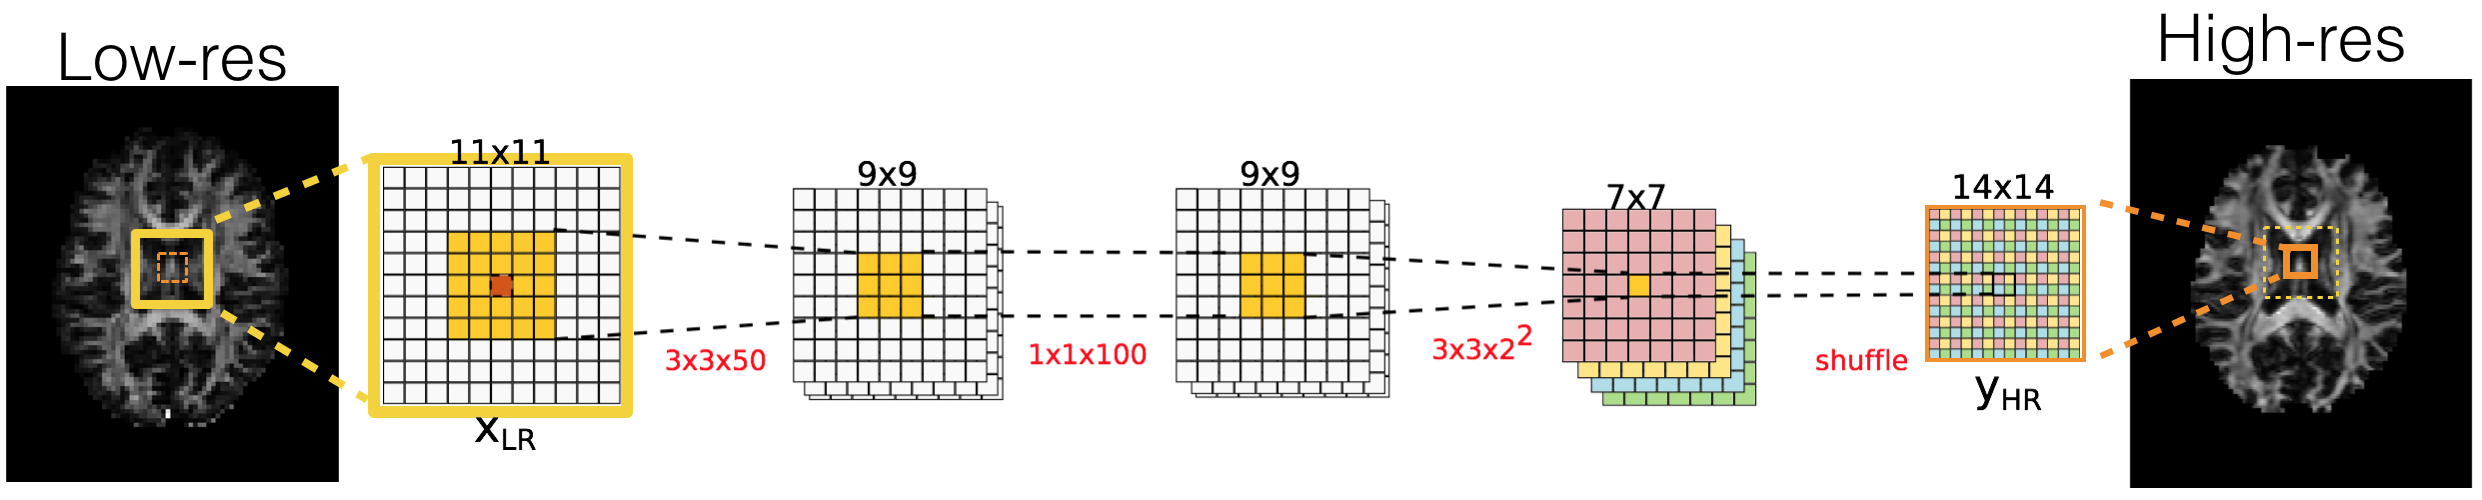
\includegraphics[width=\linewidth]{chapter_3/figures/fig_1_2.png}
	\centering	
	\caption{2D illustration of an example baseline network (ESPCN \cite{shi2016real}) with upsampling rate, $r=2$. The receptive field of the central $2^2$ pixels in the output patch is $5^2$ pixels in the input patch and
		 is shown in yellow. The shuffling operation at the end periodically rearranges the final feature maps from the low-resolution space into the high-resolution space.} 
	\label{fig:ESPCN}
	
	%\vspace{-10pt}
\end{figure}


Given training pairs of high-resolution and low-resolution patches $\mathcal{D}=\{(\mathbf{x}_i,\mathbf{y}_i)\}_{i=1}^N$, we optimise the network parameters by minimising the sum of per-pixel mean-squared-error (MSE) between the ground truth $\mathbf{y}$ and the predicted high-resolution patch $\mu_{\theta}(\mathbf{x})$ over the training set. Here $\theta$ denotes all network parameters. This is equivalent to minimising the negative log likelihood (NLL) under the Gaussian noise model $p(\mathbf{y}|\mathbf{x},\mathbf{\theta}) = \mathcal{N}(\mathbf{y}; \mu_{\theta}(\mathbf{x}), \sigma^2I)$ with fixed isotropic variance $\sigma^2$. %Using the 3D-ESPCN as the basis, in the following sections we describe methods for modelling two different types of uncertainty, namely \textit{intrinsic} and \textit{parameter uncertainty} (Fig.~\ref{fig:uncertainty_types}). 
% Here, high-resolution patches are modelled as a deterministic function of low-resolution patches corrupted by fixed isotropic noise with variance $\sigma^2$. 


\subsection{Intrinsic Uncertainty and Heteroscedastic Noise Model \label{sec:hetero}} 
\textit{Intrinsic uncertainty} quantifies the inherent ambiguity of the underlying problem that is irreducible with data as illustrated in Fig.~\ref{fig:uncertainty_types}(i). Here we capture intrinsic uncertainty by estimating the variance of the target conditional distribution $p(\mathbf{y}|\mathbf{x}, \theta)$. In medical images, intrinsic uncertainty is often spatially and channel-wise varying. For example, super-resolution could be fundamentally harder on some anatomical structures than others due to signal variability as shown in \cite{tanno2016bayesian}. It may also be the case that some channels of the image volume might contain more complex, non-linear and noisy signals than other channels e.g. higher order terms in diffusion signal representations. To capture such potential variation of intrinsic uncertainty, we model $p(\mathbf{y}|\mathbf{x}, \theta)$ as a Gaussian distribution with input-dependent varying variance: 
\begin{equation}\label{eq:hetero_pdf}
p(\mathbf{y}|\mathbf{x},\mathbf{\theta}_1, \mathbf{\theta}_2) = \mathcal{N}\big{(}\mathbf{y}; \mu(\mathbf{x};\mathbf{\theta}_1),\Sigma(\mathbf{x};\theta_2)\big{)} = \frac{\text{exp} \Big{(} \big{(}\mathbf{y}-\mu(\mathbf{x};\theta_1)\big{)}^\text{T}\Sigma^{-1}(\mathbf{x};\theta_2)\big{(}\mathbf{y}-\mu(\mathbf{x};\theta_1)\big{)}\Big{)}}{\sqrt{(2\pi)^{k} \text{det }\Sigma( \mathbf{x};\theta_2)} }
\end{equation}
 where the mean $\mu(\mathbf{x};\theta_1)$ and the covariance $\Sigma(\mathbf{x};\theta_2)$ are functions of input $\mathbf{x}$ and modelled by two separate 3D-ESPCNs (as shown in 
 Fig.~\ref{fig:hetero}), which we refer to as ``mean network'' and ``covariance network'', and are parametrised by $\theta_1$ and $\theta_2$, respectively. We note that the input patch $\mathbf{x}$ varies spatially, which makes the estimated variance spatially varying and different for respective channels. Fig.~\ref{fig:hetero} shows a 2D illustration of our 3D architecture. For each low-resolution input patch $\mathbf{x}$, we use the output of the mean network $\mu(\mathbf{x};\theta_1)$ at the top as the final estimate of the high-resolution ground truth $\mathbf{y}$ whilst the diagonal elements of the covariance $\Sigma(\mathbf{x};\theta_2)$ quantify the corresponding intrinsic uncertainty over individual components in $\mu(\mathbf{x};\theta_1)$ and over different channels. Lastly, we note that this is a specifc instance of a broad class of models, called \textit{heteroscedastic noise models} \cite{rao1970estimation,nix1994estimating} where the variance  is a function of the value of the input. In contrast, the baseline 3D-ESPCN can be viewed as an example of \textit{homoscedastic noise models} with $\mathbf{y} = \mu_{\theta}(\mathbf{x}) + \sigma \epsilon$, $\epsilon \sim \mathcal{N}(0, I)$ with constant variance $ \sigma^2$ across all spatial locations and image channels, which is highly unrealistic in most medical images. 
 

%where both mean and covariance are estimated by two separate 3D-ESPCNs $\mu_{\theta_1}(\cdot)$ and $\Sigma_{\theta_2}(\cdot)$ as functions of the input. The mean network makes predictions and the covariance network estimates the corresponding intrinsic uncertainty (see Fig. \ref{fig:heterovar}). We only use the diagonal of $\Sigma_{\theta_2}(\mathbf{x})$, which quantifies estimated intrinsic uncertainty over individual components in $\mu_{\theta_1}(\mathbf{x})$. 

%On the assumption that the model is correct (i.e. $\mu_{\theta}(\mathbf{x})$ perfectly captures the deterministic part of the super-resolution mapping) , the variance $\sigma^2$ signifies the degree of irreducible variance in the prediction of $\mathbf{y}$ given $\mathbf{x}$, and thus the \textit{intrinsic uncertainty} defined in the introduction. However, the baseline network assumes constant uncertainty across all spatial locations and image channels, which is over-simplistic for most medical images. The quality of this intrinsic uncertainty estimation is clearly limited by the likelihood form, and we need a more robust model.

% $p(\mathbf{y}|\mathbf{x},\mathbf{\theta}_1, \mathbf{\theta}_2) = \mathcal{N}(\mathbf{y}; \mu_{\theta_1}(\mathbf{x}),\Sigma_{\theta_2}(\mathbf{x}))$ where both mean and covariance are estimated by two separate 3D-ESPCNs $\mu_{\theta_1}(\cdot)$ and $\Sigma_{\theta_2}(\cdot)$ as functions of the input. The mean network makes predictions and the covariance network estimates the corresponding intrinsic uncertainty (see Fig. \ref{fig:heterovar}). We only use the diagonal of $\Sigma_{\theta_2}(\mathbf{x})$, which quantifies estimated intrinsic uncertainty over individual components in $\mu_{\theta_1}(\mathbf{x})$. 
%Brains are highly variable organs consisting of different anatomical structures. Variations in an array of factors including signals, homogeneity and frequency across the organ means that the difficulty of super-resolution depends on the neighbouhood under the network's receptive field.
\begin{figure}
	%\vspace{-20pt}
	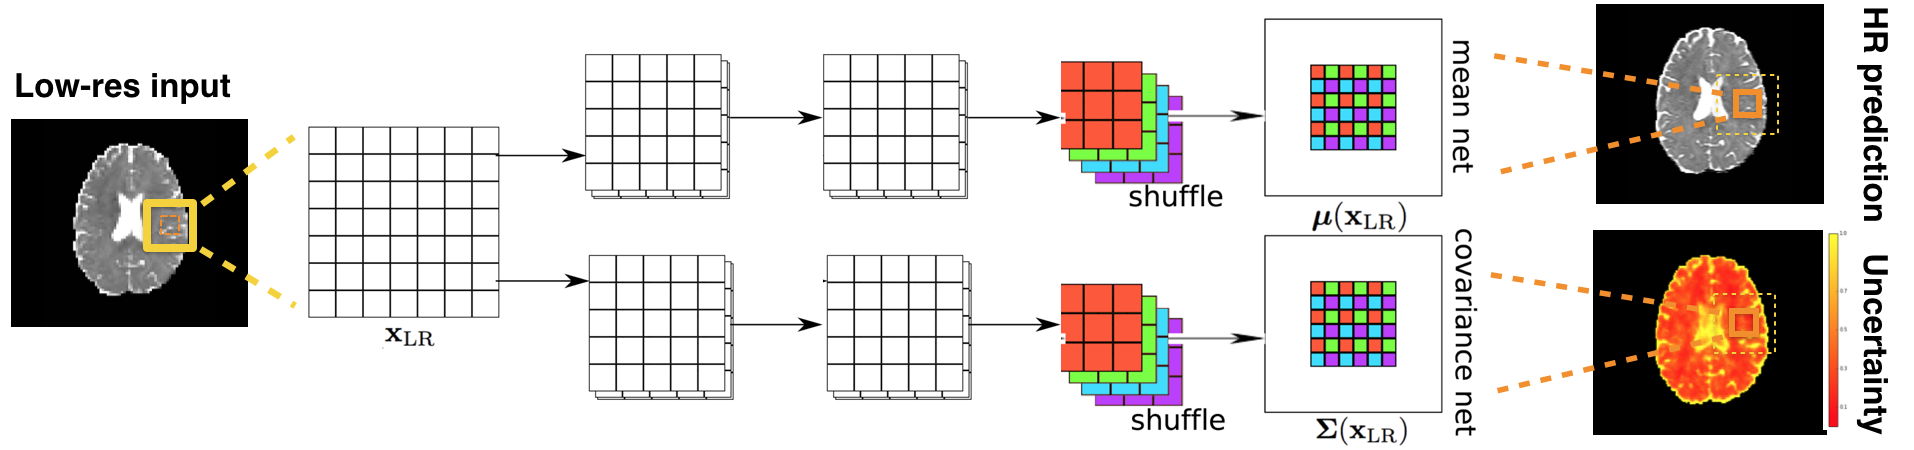
\includegraphics[width=\linewidth]{chapter_3/figures/fig_2_3.png}
	\centering	
	\caption{2D illustration of the proposed dual-path architecture which estimates the mean and diagonal covariance of the Gaussian conditional distributions as functions of the input low-resolution subvolume $\mathbf{x}$.  The ``mean network'' $\mu(\cdot)$ at the top generates the high-resolution prediction, while the ``covariance network''  $\Sigma(\cdot)$ at the bottom estimates the corresponding covariance matrix at the selected location in the volume. The diagonal entries of the covariance are used to quantify the intrinsic uncertainty. The parameters of both networks are learned by minimising the common loss function (eq.~\eqref{eq:loss_hetero}).} 
	\label{fig:hetero}
	%\vspace{-7pt}
\end{figure}

We jointly optimise the parameters $\mathbf{\theta} = \{\mathbf{\theta}_1, \mathbf{\theta}_2\}$ of the mean network and the covariance network by minimising the negative loglikelihood (NLL): 
\begin{align}
\mathcal{L}_{\theta}(\mathcal{D}) 
&= \sum_{(\mathbf{x}_i,\mathbf{y}_i)\in\mathcal{D}}- \text{log } p(\mathbf{y}|\mathbf{x},\mathbf{\theta}_1, \mathbf{\theta}_2) \\
&= \sum_{(\mathbf{x}_i,\mathbf{y}_i)\in\mathcal{D}}- \text{log } \mathcal{N}\big{(}\mathbf{y}_i; \mu(\mathbf{x}_i;\mathbf{\theta}_1),\Sigma(\mathbf{x}_i;\mathbf{\theta}_2)\big{)} \\
&= \mathcal{M}_{\theta}(\mathcal{D}) + \mathcal{H}_{\theta}(\mathcal{D}) + c \label{eq:loss_hetero}
\end{align}
where $c$ is a constant and the remaining terms are given by
\begin{equation*}
\mathcal{M}_{\theta}(\mathcal{D}) = \frac{1}{N}\sum_{i=1}^{N}\big{(}\mathbf{y}_i-\mu(\mathbf{x}_i;\theta_1)\big{)}^\text{T}\Sigma^{-1}(\mathbf{x}_i;\theta_2)\big{(}\mathbf{y}_i-\mu(\mathbf{x}_i;\theta_1)\big{)}, \quad
\mathcal{H}_{\theta}(\mathcal{D}) = \frac{1}{N}\sum_{i=1}^{N}\text{log det }\Sigma( \mathbf{x}_i;\theta_2).
\end{equation*}
Here $\mathcal{M}_{\theta}(\mathcal{D})$ denotes the mean squared Mahalanobis distance with respect to the predictive distribution $p(\mathbf{y}|\mathbf{x},\mathbf{\theta})$. For simplicity, in this work we assume diagonality of the covariance matrix $\Sigma(\mathbf{x};\theta_2)$. This means that the Mahalanobis distance term $\mathcal{M}_{\theta}(\mathcal{D})$ equates to the sum of MSEs across all pixels and channels in the output, weighted by the inverse of the corresponding variance (estimated intrinsic uncertainty)\footnote{In the case of full covariance, $\mathcal{M}_{\theta}(\mathcal{D})$ becomes the MSE in the basis of principle components, weighted by the corresponding eigenvalues.}. This term naturally encourages assigning low uncertainty to regions with higher MSEs, robustifying the training to noisy labels and outliers. On other other hand, $\mathcal{H}_{\theta}(\mathcal{D})$ represents the mean differential entropy and discourages the spread of $\Sigma_{\theta_2}(\mathbf{x})$ from growing too large. We note that the covariance network is used to modulate the training of the mean network and quantify intrinsic uncertainty during inference while only the mean network generates the final prediction, requiring a single 3D-ESPCN to perform super-resolution. 

%\textcolor{red}{The baseline 3D-ESPCN can be construed to have the trivial noise model $\mathbf{y} = \mu_{\theta}(\mathbf{x}) + \sigma \epsilon$ with $\epsilon \sim \mathcal{N}(0, I)$, where the standard deviation $ \sigma$ quantifies the intrinsic uncertainty and is assumed fixed across all spatial locations and image channels. However, this constant noise assumption is highly unrealistic; intrinsic uncertainty is likley spatially and channel-wise varying in most medical images. For example, super-resolution could be fundamentally harder on some anatomical structures than others due to signal variability. It may also be the case that some channels of the image volume might contain more complex, non-linear and noisy signals than other channels. }




%\textcolor{red}{Need to mention that the regression tree is also a heteroscedastic model, but not global model. Explain the loss attenuation - assigns higher uncertainty to regions with low uncertainty. }
%deviations between the data $\mathbf{y}$ and the mean $\mu_{\theta_1}(\mathbf{x}_i)$ under the covariance structure $\Sigma_{\theta_2}(\mathbf{x})$ while $\mathcal{H}_{\theta}(\mathcal{D})$ keeps the `spread' of $\Sigma_{\theta_2}(\mathbf{x})$ under control. 
%For example, there may be a region in the input space where super-resolution is particularly hard due to high noise or scarcity of data in training set. Minimisation of $\mathcal{L}_{\theta}(\mathcal{D})$ would then assign a larger variance to such region as desired, so its contributions to $\mathcal{M}_{\theta}(\mathcal{D})$ is minimal. 
%
%May be also mention that regressions trees are also heteroscedastic models. 
%

\subsection{Parameter Uncertainty and Variational Dropout} 
\textit{Parameter uncertainty} signifies the ambiguity in selecting the parameters of the model that best describes the training data as illustrated in Fig.~\ref{fig:uncertainty_types}.(ii). The limitation of the previously introduced 3D-ESPCN baseline (Sec.~\ref{sec:baseline}) and its heteroscedastic extension (Sec.~\ref{sec:hetero}) is their reliance on a single estimate of network parameters. In many medical imaging problems, the amount of training data is modest; in such cases, this point estimate approach increases the risk of overfitting \cite{gal2015dropout}. 

We combat this problem with a Bayesian approach. Specifically, instead of resorting to a single network of fixed parameters, we consider the (posterior) distribution over all the possible settings of network parameters given training data $p(\theta|\mathcal{D})$.  This probability density encapsulates the parameter uncertainty, with its spread of mass describing the ambiguity in selecting most appropriate models to explain the training data $\mathcal{D}$. However, in practice, the posterior $p(\theta|\mathcal{D})$ is intractable due to the difficulty in computing the normalisation constant. We, therefore, propose to approximate $p(\theta|\mathcal{D})$ with a simpler distribution $q_{\phi}(\theta)$ \cite {blei2017variational}. Specifically, we adapt a technique called \textit{variational dropout} \cite{kingma2015variational} to convolution operations from its original version introduced for feedforward NNs. 

Binary dropout \cite{srivastava2014dropout} is a popular choice of method for approximating posterior distributions \cite{gal2015dropout} with demonstrated utility in medical imaging applications \cite{worrall2016automated,yang2016fast,leibig2017leveraging,roy2019bayesian,eaton2018towards,nair2018exploring,bragman2018uncertainty}. However, typically hyper-parameters (dropout rates) need to be pre-set before the training, requiring inefficient cross-validation and thus substantially constraining the flexibility of approximate distribution family $q_{\phi}(\cdot)$ (often a fixed dropout rate per layer). This limitation motivates us to use variational dropout \cite{kingma2015variational}  that extends such approach with a way to learn the dropout rate from data for every single weight in the network and theoretically enables a more effective approximation of the posterior distribution. Another established class of methods is stochastic gradient Markov chain Monte Carlo (SG-MCMC) method \cite{neal1993bayesian,welling2011bayesian,chen2014stochastic,ma2015complete}. However, in this work, we do not not consider SG-MCMC methods because they remain, although unbiased, computationally inefficient due to the requirement of evaluating an ensemble of models for posterior computation, and are slow to converge for high-dimensional problems. 

Variational dropout \cite{kingma2015variational} employs a form of variational inference to approximate the posterior $p(\theta|\mathcal{D})$ by a member of tractable family of distributions $q_{\phi}(\theta) = \prod_{ij} \mathcal{N}(\theta_{ij}; \eta_{ij}, \alpha_{ij}\eta_{ij}^2)$ parametrised by $\phi=\{\eta_{ij}, \alpha_{ij}\}_{ij}$, such that Kullback-Leibler (KL) divergence $\text{KL} \big{(}q_{\phi}(\theta)||p(\theta|\mathcal{D})\big{)}$ is minimised. Here, $\theta_{ij}$ denotes an individual element in the convolution filters of CNNs as a random variable with parameters $\alpha_{ij}$(dropout rate) and $\eta_{ij}$ (mean), and the posterior over the set of all weights is effectively approximated with a product of univariate Gaussian distributions. In practice, introducing a prior $p(\theta)$ and applying Bayes' rule allow us to rewrite the minimization of the KL divergence as maximization of the quantity known as the evidence lower bound (ELBO) \cite{blei2017variational}. Here during training, we learn the variational parameters $\phi=\{\eta_{ij}, \alpha_{ij}\}_{ij}$ by minimizing the negative ELBO (to be consistent with the NLL cost function in eq.(3)): 
 
 \begin{equation}
\mathcal{L}_{\phi} (\mathcal{D}) =  \sum_{(\mathbf{x}_i,\mathbf{y}_i)\in\mathcal{D}} \Big{(}  \mathbb{E}_{q_{\phi}(\theta)}[- \text{log }p(\mathbf{y}_i|\mathbf{x}_i,\theta)]   +  \text{KL} (q_{\phi}(\theta)||p(\theta))\Big{)}
 \end{equation}
An accurate approximation for the KL term for log-uniform prior $p(\theta)$ is proposed in \cite{molchanov2017variational}, which is employed here. On the other hand, the first term (referred to as the reconstruction term) cannot be computed exactly, thus we employ the following MC approximation by sampling $S$ samples of network parameters from the posterior:
\begin{equation}\label{eq:reconstruction}
\mathbb{E}_{q_{\phi}(\theta)}[- \text{log }p(\mathbf{y}|\mathbf{x},\theta)] \approx \frac{1}{S}\sum_{s=1}^{S} - \text{log }p(\mathbf{y}|\mathbf{x},\theta^{(s)}), \quad \theta^{(s)} \sim q_{\phi}(\theta)
\end{equation}
Adapting the local reparametrisation trick presented in \cite{kingma2015variational} to a convolution operation, we derive the implementation of posterior sampling $\theta^{(s)} \sim q_{\phi}(\theta)$ such that the variance of gradients over each mini-batch is low \footnote{See the proof for feedforward networks given in  \cite{kingma2015variational} which generalises to convolutions}. In practice, this amounts to replacing each standard convolution kernel with a ``Bayesian'' convolution, which proceeds as follows. Firstly, we define two separate convolution kernels: $\mathbf{\eta} \in \mathbb{R}^{c\times k^2}$ (``mean'' kernels) and $\alpha \odot \eta^{2} \in \mathbb{R}^{c\times k^2}$ (``variance'' kernels) where $ \odot $ denotes the element-wise multiplication, $c$ is the number of input channel and $k$ is the kernel width. Input feature maps $F_{\text{in}}$ and its elementwise squared values are convolved by respective kernels to compute the ``mean'' and ``variance'' of the output feature maps $\mu_{Y}\delequal F_{\text{in}} \star \mathbf{\eta}$ and $\sigma^{2}_{Y} \delequal F_{\text{in}}^2\star (\alpha \odot \eta^{2})$. Lastly, the final output feature maps $F_{\text{out}}$ are computed by drawing a sample from $\mathcal{N}(\mu_{Y}, \sigma^{2}_{Y})$ i.e. computing the following quantity: 
\begin{equation}\label{eq:noise_injection}
F_{\text{out}} \delequal \mu_{Y} +  \sigma_{Y} \odot \mathbf{\epsilon}, \quad \mathbf{\epsilon} \sim \mathcal{N}(0,I).
\end{equation}
Every forward pass (i.e. computation of each $p(\mathbf{y}|\mathbf{x},\theta^{(s)})$) with variational dropout is thus performed via a sequence of Bayesian convolutions.  Since the injected Gaussian noise $\epsilon$ is independent of the variational parameters $\phi=\{\eta_{ij}, \alpha_{ij}\}_{ij}$, the approximate reconstruction term in eq.~\ref{eq:reconstruction} is differentiable with respect to them \cite{kingma2013auto}.  

%input features maps are convolved with separate "mean" and "covariance" filters and summed at the end (see Fig.\ref{fig:vd_lrt_1}



%Dropout is a popular class of techniques for controlling overfitting in modern deep learning, and has become a method of choice for estimating posterior distribution in the medical imaging applications \cite{worrall2016automated,yang2016fast,leibig2017leveraging}. However, typically hyper-parameters (dropout rates) need to be pre-set before the training, requiring inefficient cross-validation and thus substantially constraining the flexibility of approximate distribution family $q_{\phi}(\cdot)$ (often a fixed dropout rate per layer). By contrast, variational dropout offers a way to tune the dropout rates from data for each weight and theoretically enables a more effective approximation of the posterior. Another established class of approximate inference methods for Bayesian NNs is stochastic gradient Markov chain Monte Carlo (SG-MCMC) method \cite{neal1993bayesian,welling2011bayesian,chen2014stochastic,ma2015complete}. In this work, we did not consider SG-MCMC methods because they remain, although unbiased, computationally inefficient due to the requirement of evaluating an ensemble of models for posterior computation, and slow convergence rate in high-dimensional problems. 

%{\color{red}Daniel's version of the variational inference section: The limitation of the two previous models is their reliance on a single estimate of the network parameters. In practice, there is more than one set of parameters that best explain the data. The Bayesian solution to this problem is to average over all possible model predictions from all possible settings of the parameters, weighting each by the (posterior) probability of the parameters given the training data  $p(\mathbf{y}|\mathbf{x}, \mathcal{D}) = \int p(\mathbf{y}|\mathbf{x}, \omega, \mathcal{D}) p(\omega|\mathcal{D})\,\mathrm{d}\omega$. Here $p(\mathbf{y}|\mathbf{x}, \omega, \mathcal{D}$ represented the likelihood function of the CNN and $p(\omega | \mathcal{D})$ is the posterior of the network parameters $\omega$ given the data. 
%
%In practice, this is an intractable integral for two reasons, 1) the likelihood function is too complicated for the integral to be computed in closed form, 2) evaluation of the posterior is intractable. The solution to 1) is to Monte Carlo sample the integral, the solution to 2) is to approximate $p(\omega|\mathcal{D})$ with a simpler, parameterised approximation $q_{\phi}(\omega)$. The approximate posterior is found by minimsing the KL-divergence $D_{\text{KL}}(q_{\phi}(\omega)||p(\omega|\mathcal{D}))$. Since the posterior is intractable, we can expand using Bayes' Rule to get the `variational lower bound $\mathbb{E}_{q_{\phi}(\omega)}[\log p(\mathbf{y}|\mathbf{x}, \omega)] - D_{\text{KL}}(q_{\phi}(\omega)||p(\omega))$, where $p(\omega)$ is the prior on the parameters. In `variational dropout', the prior is taken to be a log-uniform distribution and the approximate posterior is a spherical Gaussian distribution, see \cite{kingma2015variational} for details on the form of the variational lower-bound.}

% 
%% %%%% DO NOT DELETE (ILLUSTRATION OF VARIATIONAL CONVOLUTION)
%%\begin{figure}[ht]
%%	%\vspace{-2em}
%%	\centering
%%	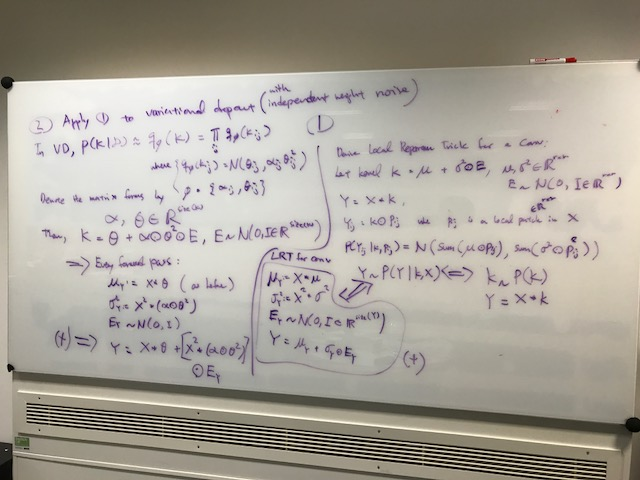
\includegraphics[width=15cm]{chapter_3/figures/fig_11.JPG}
%%	\small
%%	\caption{Local reparametrization trick for variational dropout for a convolution layer} 
%%	\label{fig:vd_lrt_1}
%%	%	\vspace{-1em}
%%\end{figure}
%
%
%
\subsection{Joint Modelling of Intrinsic and Parameter Uncertainty}
We now describe how to combine the methods for modelling intrinsic and parameter uncertainty. Operationally, we take the dual architecture (Fig.~\ref{fig:hetero}) used to model intrinsic uncertainty, and apply variational dropout to every convolution layer in it. The intrinsic uncertainty is modelled in the heteroscedastic Gaussian model $p(\mathbf{y}|\mathbf{x}, \theta_1, \theta_2) = \mathcal{N}\big{(}\mathbf{y}; \mu(\mathbf{x};\theta_1),\Sigma(\mathbf{x};\theta_2)\big{)}$ while the parameter uncertainty is captured in the approximate posterior $q_{\phi}(\theta_1, \theta_2) \approx p(\theta_1, \theta_2|\mathcal{D}) $ obtained from variational dropout. 

 At test time, for each low-resolution input subvolume $\mathbf{x}$, we would like to compute the predictive distribution $p(\mathbf{y}|\mathbf{x}, \mathcal{D})$ over the high-resolution output $\mathbf{y}$. We approximate this quantity by $q_\phi^*(\mathbf{y}|\mathbf{x})$ by taking the ``average'' of all possible network predictions $p(\mathbf{y}|\mathbf{x}, \theta)=\mathcal{N}\big{(}\mathbf{y}; \mu(\mathbf{x};\theta_1),\Sigma(\mathbf{x};\theta_2)\big{)} $ from all settings of the parameters $\theta_1, \theta_2$, weighted by the associated approximate posterior distribution $q_{\phi}(\theta_1, \theta_2)$. More formally, we need to compute the integral below:
\begin{align} 
q_\phi^*(\mathbf{y}|\mathbf{x}) &\delequal  \int \underbrace{\mathcal{N}(\mathbf{y}; \mu(\mathbf{x};\theta_1),\Sigma(\mathbf{x};\theta_2))) }_{\text{Network prediction}}\cdot \underbrace{q_{\phi}(\theta_1, \theta_2)}_{\text{Approx. posterior}}  \mathrm{d}\theta_1  \mathrm{d}\theta_2  \label{eq:full_distribution} \\
& \approx \int p(\mathbf{y}|\mathbf{x}, \theta_1, \theta_2)\cdot p(\theta_1, \theta_2|\mathcal{D})  \mathrm{d}\theta_1 \mathrm{d}\theta_2 = p(\mathbf{y}|\mathbf{x}, \mathcal{D})  
\end{align}
where the last line represents the true predictive distribution $p(\mathbf{y}|\mathbf{x}, \mathcal{D})$ which is estimated by our model $q_\phi^*(\mathbf{y}|\mathbf{x})$. However, in practice, the integral $q_\phi^*(\mathbf{y}|\mathbf{x})$ cannot be evaluated in closed form because the likelihood $\mathcal{N}\big{(}\mathbf{y}; \mu(\mathbf{x};\theta_1),\Sigma(\mathbf{x};\theta_2)\big{)}$ is a highly non-linear function of input $\mathbf{x}$ as given in eq.~\ref{eq:hetero_pdf}. At test time, we therefore estimate, for each input $\mathbf{x}$, the mean and covariance of the approximate predictive distribution $q_\phi^*(\mathbf{y}|\mathbf{x})$ with the unbiased Monte Carlo estimators: 
\vspace{-3mm}
\begin{align}
\hat{\mu}_{\mathbf{y}|\mathbf{x}}&\delequal \frac{1}{T}\sum_{t=1}^T\mu(\mathbf{x};\theta_{1}^{t}) \label{eq:est_mean} \xrightarrow[T\rightarrow\infty]{}\mathbb{E}_{q_\phi^*(\mathbf{y}|\mathbf{x})} [\mathbf{y}]\\
\hat{\Sigma}_{\mathbf{y}|\mathbf{x}} &\delequal \frac{1}{T} \sum_{t=1}^T\Big{(}\Sigma(\mathbf{x};\theta_{2}^{t})+\mu(\mathbf{x};\theta_1^t)\mu(\mathbf{x};\theta_1^t)^{\text{T}}\Big{)}-\hat{\mu}_{\mathbf{y}|\mathbf{x}} \hat{\mu}_{\mathbf{y}|\mathbf{x}}^{\text{T}}\xrightarrow[T\rightarrow\infty]{}\text{cov}_{q_\phi^*(\mathbf{y}|\mathbf{x})} [\mathbf{y}, \mathbf{y}]
\label{eq:est_cov}
\end{align}
where $\{(\theta^t_1,\theta^t_2)\}_{t=1}^T$ are samples of the network parameters (i.e. convolution kernels) drawn from the approximate posterior $ q_{\phi}(\theta_1, \theta_{2})$. In the other words, the inference performs $T$ stochastic forward passes at test time by injecting noise into features according to eq.~\ref{eq:noise_injection}, and amalgamates the corresponding network outputs to compute the sample mean $\hat{\mu}_{\mathbf{y}|\mathbf{x}}$ and sample covariance $\hat{\Sigma}_{\mathbf{y}|\mathbf{x}}$. We use the sample mean $\hat{\mu}_{\mathbf{y}|\mathbf{x}}$  as the final prediction of an high-resolution ouput patch $\mathbf{y}$ and use the diagonal elements of the sample covariance $\hat{\Sigma}_{\mathbf{y}|\mathbf{x}}$ to quantify the corresponding uncertainty, which we refer to as \textit{predictive mean} and \textit{predictive uncertainty}, respectively. 

%When we use the baseline 3D-ESPCN, the first term in the sample variance reduces to $\sigma^2I$, which is equivalent to homogeneous intrinsic noise. 


\begin{figure}
	%\vspace{-20pt}
	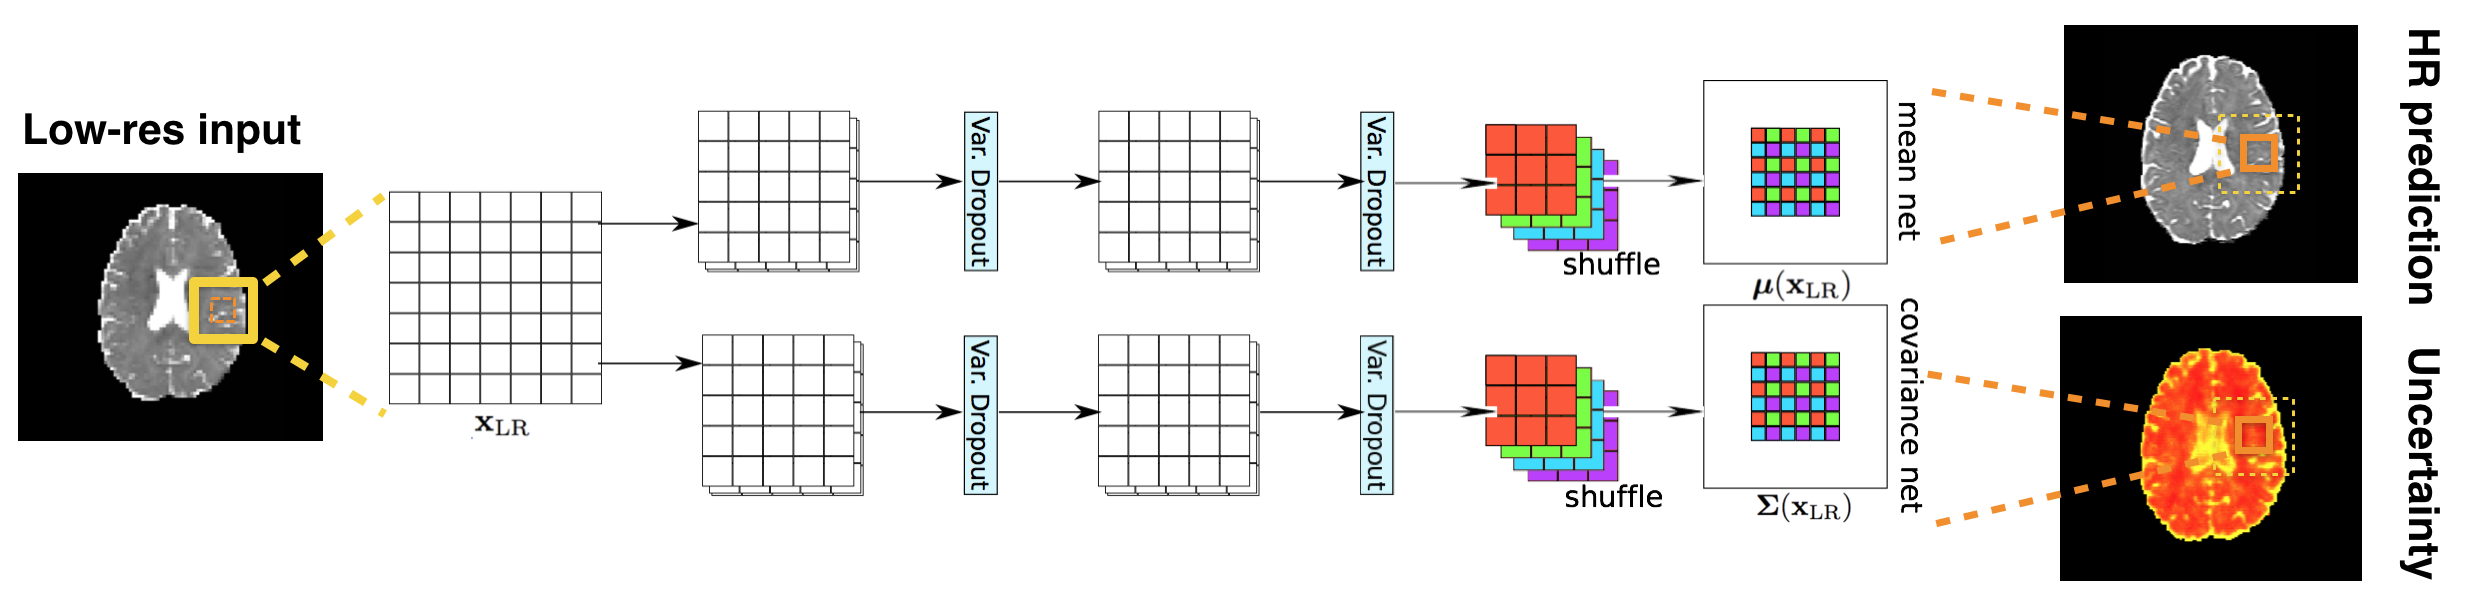
\includegraphics[width=\linewidth]{chapter_3/figures/fig_2_2.png}
	\centering	
	\small 
	\vspace{-8mm}
	\caption{\small 2D illustration of a heteroscedastic network with variational dropout. Diagonal covariance is again assumed. The top 3D-ESPCN estimates the mean and the bottom one estimates the covariance matrix of the likelihood. Variational dropout is applied to feature maps after every convolution where Gaussian noise is injected into feature maps $F_{\text{out}} = \mu_{Y} +  \sigma_{Y} \odot \mathbf{\epsilon}$ where $\mathbf{\epsilon} \sim \mathcal{N}(0,I)$ (see eq.~\ref{eq:noise_injection}). } 
	\label{fig:heterovar}
	%\vspace{-7pt}
\end{figure}

\subsection{Uncertainty Decomposition and Propagation} \label{sec:uncertainty_decom}
Predictive uncertainty arises from the combination of two source effects, namely intrinsic and parameter uncertainty, for which we have previously introduced methods for estimation. Lastly, we introduce a method based on variance decomposition for disentangling these effects and quantifying their contributions separately in predictive uncertainty. We consider such decomposition problem in the presence of an arbitrary transformation of the output variable $\mathbf{y}$. 

The users of super-resolution algorithms are often interested in the quantities that are derived from the predicted high-resolution images, rather than the images themselves. For example, quantities such as the principal direction (first eigenvalue of the DT), mean diffusivity (MD) and fractional anisotropy (FA) are typically calculated from diffusion tensor images (DTIs) and used in the downstream analysis. We therefore consider an generic function\footnote{We assume here that the transform $g$ is a measurable function with well-defined expectation and variance.} $g:\mathcal{Y}\rightarrow\mathbb{R}^{m}$ which transforms the high-resolution multi-channel data $\mathbf{y}$ to a quantity of interest e.g. MD and FA maps, and propose a way to propagate the predictive uncertainty over $\mathbf{y}$ to the transformed domain (i.e. compute the variance of $p(g(\mathbf{y})|\mathcal{D}, \mathbf{x})$) and decompose it into the ``intrinsic'' and ``parameter'' components. Specifically, by using the law of total variance \cite{weiss2006course}, we perform the following decomposition:

%\begin{align}
%\mathbb{V}_{p(\mathbf{y}|\mathbf{x},\mathcal{D})} [g(\mathbf{y})]
%& =  %\mathbb{E}_{p(\theta|\mathcal{D})}\big{[}\mathbb{V}_{p(g(\mathbf{y})|\theta,\mathbf{x},\mathcal{D})}[g(\mathbf{y})]-\mathbb{V}_{p(g(\mathbf{y})|\theta,\mathbf{x},\mathcal{D})}[g(\mathbf{y})|\theta]\big{]} + \mathbb{E}_{p(\theta|\mathcal{D})}\big{[}\mathbb{V}_{p(g(\mathbf{y})|\theta,\mathbf{x},\mathcal{D})}[g(\mathbf{y})|\theta]\big{]}\\
%&=\underbrace{\mathbb{V}_{p(\theta|\mathcal{D})}[\mathbb{E}_{p(g(\mathbf{y})|\theta,\mathbf{x},\mathcal{D})}[g(\mathbf{y})|\theta]]}_{\text{propagated parameter uncertainty}} +   \underbrace{\mathbb{E}_{p(\theta|\mathcal{D})}[\mathbb{V}_{p(g(\mathbf{y})|\theta,\mathbf{x},\mathcal{D})}[g(\mathbf{y})|\theta]]}_{\text{propagated intrinsic uncertainty}} \\
%&= \Delta_{m}(g(\mathbf{y})) + \Delta_{i}(g(\mathbf{y}))  
%\label{eq:variance_decomposition}
%\end{align}

\begin{equation}
\mathbb{V}_{p(\mathbf{y}|\mathbf{x},\mathcal{D})} [g(\mathbf{y})] = \Delta_{m}(g(\mathbf{y})) + \Delta_{i}(g(\mathbf{y}))  
\label{eq:variance_decomposition}
\end{equation}
where the respective component terms are given by:
\begin{align}
\Delta_{m}(g(\mathbf{y})) & = \mathbb{E}_{p(\theta|\mathcal{D})}\big{[}\mathbb{V}_{p(g(\mathbf{y})|\theta,\mathbf{x},\mathcal{D})}[g(\mathbf{y})]-\mathbb{V}_{p(g(\mathbf{y})|\theta,\mathbf{x},\mathcal{D})}[g(\mathbf{y})|\theta]\big{]} \\
&=\underbrace{\mathbb{V}_{p(\theta|\mathcal{D})}[\mathbb{E}_{p(g(\mathbf{y})|\theta,\mathbf{x},\mathcal{D})}[g(\mathbf{y})|\theta]]}_{\text{propagated parameter uncertainty}} 
\\
\Delta_{i}(g(\mathbf{y}))  &=   \underbrace{\mathbb{E}_{p(\theta|\mathcal{D})}[\mathbb{V}_{p(g(\mathbf{y})|\theta,\mathbf{x},\mathcal{D})}[g(\mathbf{y})|\theta]]}_{\text{propagated intrinsic uncertainty}} 
\end{align}
We refer to the components $ \Delta_{m}(g(\mathbf{y})) $ and $ \Delta_{i}(g(\mathbf{y})) $ as ``propagated'' parameter and intrinsic uncertainty.  Intuitively, the first term quantifies the difference in variance between the cases where we have variable parameters and fixed parameters. In other words, this quantifies how much predictive uncertainty on the derived quantity arises, on average, from the variability in parameters. The second term on the other hand quantifies the average variance of the model prediction when the parameters are fixed, which signifies the model-independent uncertainty due to data i.e. intrinsic uncertainty.  Assuming that the considered neural network is identifiable\footnote{We note that a neural network is, in general, not identifiable i.e. there exist more than a single set of parameters that capture the same target distribution $p(g(\mathbf{y})|\mathbf{x})$. In such cases, the posterior distribution $p(\theta|\mathcal{D})$ does not collapse to a single Dirac Delta function with infinite amount of observations---it rather converges to a mixture of all sets of network parameters $\Theta$  such that $p(g(\mathbf{y})|\theta^{*},\mathbf{x}) = p(g(\mathbf{y})|\mathbf{x}) \forall \theta^{*} \in \Theta $. However, the expectation $\mathbb{E}_{p(g(\mathbf{y})|\theta,\mathbf{x},\mathcal{D})}[g(\mathbf{y})|\theta]$ is the same for all $\theta \in \Theta$ and thus the propagated parameter uncertainty $ \Delta_{m}(g(\mathbf{y}))$ converges to zero. } and sufficiently complex to capture the underlying data generating process, as the amount of training data increases, the posterior $p(\theta|\mathcal{D})$ tends to a Dirac delta function and thus the first term diminishes to zero while the second term remains. A similar variance decomposition technique was employed in \cite{bowsher2012identifying} to understand how the variation in cell signals of interest (e.g. gene expression) in a bio-chemical network is caused by the fluctuations of other environmental variables (e.g. transcription rate and biological noise). In our case, we employ the variance decomposition technique to separate the effects of network parameters from the intrinsic uncertainty in the prediction of $g(\mathbf{y})$.  

%In statistics \cite{weiss2006course}, the two terms are described as the variance components  ``explained'' and ``unexplained'' by the model parameters.

We first consider a special case where the transform $g$ is an identify map i.e. $g(\mathbf{y})=\mathbf{y}$. Assuming the likelihood is modelled by a Gaussian distribution with heteroscedastic noise i.e. $p(\mathbf{y}|\theta_1, \theta_2, \mathbf{x},\mathcal{D}) = \mathcal{N}(\mathbf{y}; \mu(\mathbf{x};\theta_1),\Sigma(\mathbf{x};\theta_2))$, then we can show that the parameter and intrinsic uncertainty are given by
\begin{equation}
\Delta_{m}(\mathbf{y}) = \mathbb{V}_{p(\theta_{1}|\mathcal{D})}[\mu_{\theta_1}(\mathbf{x})], \quad \Delta_{i}(\mathbf{y})  =  \mathbb{E}_{p(\theta_{2}|\mathcal{D})}[\Sigma_{\theta_2}(\mathbf{x})]
\end{equation}
which can be approximated by the components of the MC variance estimator in eq.~\eqref{eq:est_cov} :
\begin{align}\label{eq:sampler_mean}
\widehat{\Delta}_{m}(\mathbf{y})  &=\frac{1}{T} \sum_{t=1}^T\mu(\mathbf{x};\theta_1^t)\mu(\mathbf{x};\theta_1^t)^{\text{T}} -\hat{\mu}_{\mathbf{y}|\mathbf{x}} \hat{\mu}_{\mathbf{y}|\mathbf{x}}^{\text{T}}\\ 
\widehat{\Delta}_{i}(\mathbf{y})  &= \frac{1}{T} \sum_{t=1}^T\Sigma(\mathbf{x};\theta_{2}^{t}) \label{eq:sampler_var}
\end{align}
where $\{(\theta^t_1,\theta^t_2)\}_{t=1}^T$ are drawn from the approximate posterior $q_{\phi}(\theta_1, \theta_{2})$. %If you turn off the variaitional dropout in the covariance network, the intrinsic uncertainty term reduces to $\Delta_{i}(\mathbf{y}) = \Sigma_{\theta_2^*}(\mathbf{x})$ where $\theta_2^*$ denotes the point-estimate of parameters in the covariance network. 

%\textcolor{red}{Food for thought: May be you can generalise this argument for transforms $g$ of specific types e.g. low-variance estimators similar to eq. \eqref{eq:sampler_mean} and eq. \eqref{eq:sampler_var} when $g$ additively or multiplicatively separates model parameters $\theta$ between heteroschedastic noise and posterior distribution? e.g. MD is a good example }.

More generally, when the transform $g$ is complicated, MC sampling provides an alternative implementation. Given samples of model parameters $\{\theta_{t}\}_{t=1}^{T} \sim q(\theta|\mathcal{D})$ and $\{g^{t}_{j}\}_{j=1}^J \sim p(g(\mathbf{y})|\theta_{t},\mathbf{x},\mathcal{D})$ for $t=1, ...,T$,  we estimate both the progapated parameter and intrinsic uncertainty as follows:

% Before bessel's correction
%\begin{align}
%\widehat{\Delta}_{m}(g(\mathbf{y}))  &\delequal \frac{1}{T}\sum_{t}(\hat{\mu}^{t})^2  - \Big{(}\frac{1}{JT}\sum_{j,t}(g^{t}_{j}) \Big{)}^2 \label{eq:mc_model_uncertainty} \\ 
%\widehat{\Delta}_{i}(g(\mathbf{y}))  &\delequal  \frac{1}{JT}\sum_{j,t}(g^{t}_{j})^2 - \frac{1}{T}\sum_{t}(\hat{\mu}^{t})^2 \label{eq:mc_intrinsic_uncertainty} \\
%\hat{\mu}^{t} & = \frac{1}{J}\sum_{j}g^{t}_{j}
%\end{align}

\begin{align}
\widehat{\Delta}_{m}(g(\mathbf{y}))  &\delequal \frac{1}{T}\sum_{t}(\hat{\mu}^{t})^2  - \Big{(}\frac{1}{(J-1)T}\sum_{j,t}(g^{t}_{j}) \Big{)}^2 \label{eq:mc_model_uncertainty} \\ 
\widehat{\Delta}_{i}(g(\mathbf{y}))  &\delequal  \frac{1}{(J-1)T}\sum_{j,t}(g^{t}_{j})^2 - \frac{1}{T}\sum_{t}(\hat{\mu}^{t})^2 \label{eq:mc_intrinsic_uncertainty} \\
\hat{\mu}^{t} & = \frac{1}{J}\sum_{j}g^{t}_{j}. 
\end{align}
These estimators are, although unbiased, higher in variance than the case where $g$ is the identity (eq.~\eqref{eq:sampler_mean} and eq.~\eqref{eq:sampler_var}), due to two sources of sampling, thus requiring more samples for reliable estimation of respective uncertainty components. 

%\textcolor{red}{These estimators are biased at the moment - need to check this properly but should be fine just to replace $J$ with $J-1$. Also, we should mention that these estimators are high in variance due to two sources of sampling, and requires more samples than eq. \eqref{eq:sampler_mean} and eq. \eqref{eq:sampler_var}}.


% ---------------- Experiments ----------------------------
\section{Experiments and Results}

In this section, we evaluate the proposed uncertainty modelling techniques for super-resolution of diffusion MR images. We first compare quantitatively the reconstruction performance of our probabilistic CNN models against the relevant baselines in two different types of diffusion signal representations. Secondly, we study the real-world utility of the technique in downstream tractography applications. Thirdly, we evaluate the value of predictive uncertainty as a realiability metric of output images on multiple datasets of both healthy subjects and those with unseen pathological structures such as brain tumour (Glioma) and multiple sclerosis (MS). 

%Lastly, we decompose the measure of predictive uncertainty into the intrinsic and parameter components, and correlate them to the prediction accuracy on a HCP healthy subject with benign abnormalities.  \textcolor{red}{come back to this after modifying the section \ref{sec:unseen_abnormality}}


% We 

%This section focuses on the task of diffusion MRI super-resolution and evaluates the utility of the proposed uncertainty modelling techniques in terms of reconstruction accuracy and risk management of preditive failures. The accuracy of the baseline CNN architecture (3D-ESPCN) and its probabilistic extensions are compared against standard interpolation techniques and random-forest implementations of IQT \cite{alexander2017image,tanno2016bayesian}. In particular, we demonstrate on two different types of diffusion MR images, namely diffusion tensor images (DTIs) and Mean Apparent Propagator (MAP)-MRI \cite{ozarslan2013mean}. We also study the effects of uncertainty modeling on generalisability by testing on the Lifespan dataset, which differs from the training data in acquisition protocl and population range. We additionally test the utility of improved model accuracy in downstream tractography applications. We then study how the value of predictive uncertainty provides an indicator of predictive accuracy on images of both healthy subjects and brain tumour patients. Lastly, we decompose the measure of predictive uncertainty into the intrinsic and parameter components, and correlated them to the model performance on the DTI of a HCP healthy subject with benign abnormalities.

\subsection{Datasets} \label{sec:dataset}
We make use of the following four diffusion MRI datasets to evaluate different benefits of the proposed technique: 

\begin{itemize}
	\item \textbf{Human Connectome Project dataset: } we use the diffusion MRI data from the WU-Minn HCP (release Q3) \cite{van2013wu} as the source of the training datasets. The dataset enjoys very high image resolution, signal levels and coverage of the measurement space, enabled by the combination of custom imaging, reconstruction innovations and a lengthy acquisition protocol \cite{sotiropoulos2013advances}. Each subject's data set contains $288$ diffusion weighted images (DWIs) of voxel size $1.25^{3} \text{ mm}^{3}$ of which $18$ have nominal $b=0$ and the three high-angular-resolution-diffusion-imaging (HARDI) shells of 90 directions have nominal b-values of $1000, 2000$, and $3000 \text{ smm}^{-2}$ (see \cite{sotiropoulos2013advances} for the full acquisition details). The data are preprocessed by correcting distortions including susceptibility-induced, eddy currents and motion as outlined in \cite{glasser2013minimal}.
	
	\item \textbf{Lifespan dataset:} this dataset (available online at \url{http://lifespan.humanconnectome.org} contains $26$ subjects of much wider age range ($8-75$ years) than the main HCP cohorts ($22-36$ years), and is acquired with a shortened version of the main HCP protocol with lower resolution ($1.5$ mm isotropic voxels) and only two HARDI shells, with $b = 1000$ and $2500 \text{ smm}^{-2}$. However, we also note that the protocol still leverages the special features of the HCP scanners, providing images of substantially better quality than standard sequences. We utilise this out-of-training-distribution dataset  to assess the robustness of our techniques to domain shifts. 
	 
	\item \textbf{Prisma dataset:} two healthy male adults (29 and 33 years old respectively) were scanned twice at different image resolutions using the clinical 3T Siemens Prisma scanner in FMRIB, Oxford. Both datasets contain diffusion MRI data with 21 $b=0$ images and three 90-direction HARDI shells, b-values of 1000, 2000, and $3000 \text{ smm}^{-2}$, each for two resolutions, 2.50 mm and 1.35 mm isotropic voxels  (see \cite{alexander2017image} for full acquisition details). In addition, each of these datasets also includes a standard 3D T1-weighted MPRAGE (1 mm isotropic resolution). The Prisma scanner is less powerful than the bespoke HCP scanner and cannot achieve sufficient signal at $1.25$ mm resolution, but the $1.35$ mm data provides a pseudo ground-truth for IQT resolution enhancement of the 2.5 mm data. 
	
	\item  \textbf{Pathology dataset:} we use two separate datasets which consist of images of brain tumour (Glioma) \cite{figini2018prediction} and multiple sclerosis (MS) patients, respectively. The data of each wubject with glioma contains DWIs with $b=700 \text{ s/mm}^2$ while the measurement of each MS patient is of $b=1200 \text{ s/mm}^2$. Both datasets have isotropic voxel size $2^3 \text{ mm}^3$, which is closer to the image resolution of commonplace clinical scanners. We use these datasets to assess the behaviour of predictive uncertainty on images with pathological features that are not represented in the training data set.
\end{itemize}

In all the experiments, super-resolution are performed on diffusion parameter maps derived from the DWIs in the above datasets. In particular, we consider two diffusion MRI models, namely the diffusion tensor (DT) model \cite{basser1994mr} and Mean Apparent Propagator (MAP) MRI \cite{ozarslan2013mean}, where the former is the simplest and most standard diffusion parameter map, and the latter is a high-order generalisation of the former with the capacity to characterise signals from more complex tissue structures (e.g. fibre crossing regions), a requirement for successful tractography applications. We compute both of these diffusion parameter maps using the implementation from \cite{alexander2017image}, which is available at \url{https://github.com/ucl-mig/iqt}. 

We fit the DT model to the combination of $b=0$ images and $b=1000  \text{ s/mm}^2$ HARDI shell for the HCP and Lifespan datasets, and $b=700  \text{ s/mm}^2$ shell for the brain tumour dataset. In all cases, weighted linear least squares are employed for the fitting, taking into account the spatially varying b-values and gradient directions in the HCP dataset. On the other hand, in the case of MAP-MRI, $22$ coefficients of basis functions up to order $4$ are estimated via (unweighted) least squares to all three shells of the HCP, Lifespan and Prisma datasets. As noted in \cite{alexander2017image}, the choice of scale parameters (see \cite{ozarslan2013mean}) $\mu_{x} = \mu_{y} = \mu_{z} = 1.2\times 10^{-3}$ mm empirically minimises the fitting error in the HCP dataset, and is used for all datasets. 

Training datasets in all experiments are constructed by artificially downsampling very high-resolution images in the HCP dataset. In particular, we employ the following downsampling procedure: (i) the raw DWIs of selected subjects are blurred by applying the mean filter of size $r\times r \times r$ independently over channels with $r$ denoting the upsampling rate; (ii)  the DT or MAP parameters are computed for every voxel; (iii) the spatial resolution of the resultant parameter maps are reduced by taking every $r$ pixels. A coupled library of low-resolution and high-resolution patches is then constructed by associating each patch in the downsampled DTI/MAP-MRI with the corresponding patch in the ground truth DTI or MAP-MRI. In this case, we ensure the low-resolution patch to be centrally and entirely contained within the corresponding high-resolution patch (as illustrated by the yellow and orange squares in Fig.~\ref{fig:ESPCN}). We then randomly select a pre-set number of patches from each subject in the training pool to create a training dataset as detailed in Table~\ref{tab:train_data}. In addition to the $8$ subjects used in the prior work \cite{alexander2014image,tanno2016bayesian,tanno2017bayesian}, we randomly select additional $8$ subjects from the HCP cohort and include them in the training subject pool. Patches are standardized channel-wise by subtracting the mean of foreground pixel intensities of the corresponding subject and dividing by its standard deviation. Moreover, since MAP-MRI datasets contain outliers due to model fitting, in large enough quantity to influence the training of the baseline 3D-ESPCN model, we remove them by clipping the voxel intensity values of the respective $22$ channels separately at $0.1\%$ and $99.9\%$ percentiles computed over all the foreground voxels in the whole training dataset. 

\begin{table}
	\caption{Details of training data for two diffusion MR signal representations, DTIs and MAP-MRIs. The first two columns from the right denote the size of the input $\mathbf{x}$ and output patches $\mathbf{y}$ of dimension $[\text{width}, \text{height}, \text{depth}, \text{channels}]$ while the third and the fourth columns show the number of patch pairs $(\mathbf{x}, \mathbf{y})$ extracted from each subject, and the total number of training subjects used, respectively. }
	\center
	\small
	\begin{tabular}{lclclclc|cl}
		\hline
		Data &  Size of input $\mathbf{x}$ &Size of output $\mathbf{y}$ &  No. pairs $(\mathbf{x}, \mathbf{y})$ per subject& No. subjects   \\ 
		\hline	
		DTIs &  $11\times 11 \times 11 \times 6$  & $14\times 14 \times 14 \times 6$  & $8000$ & $16$   \\
		MAP-MRIs  & $21\times 21 \times 21 \times 22$  & $14\times 14 \times 14 \times 22$  & $4000$ & $16$  \\
		
		\hline
		\label{tab:train_data}
	\end{tabular}%	
	\vspace{-5mm}

\end{table}


\subsection{Network Architectures and Training}
For the training of all CNN models, we minimised the associated loss function using Adam \cite{kingma2014adam} for $200$ epochs with initial learning rate of $10^{-3}$ and $\beta= [ 0.9, 0.999]$, with minibatches of size $12$. We hold out 50\% of training patch pairs as a validation set. The best performing model was selected based on the mean-squared-error (MSE) on the validation set. 

For the super-resolution of DTIs, as in \cite{shi2016real}, we use a minimal architecture for the baseline 3D-ESPCN, consisting of three $3D$ convolutional layers with filters $(3^3,50)\to(1^3,100)\to(3^3,6r^3)$ where $r$ is upsampling rate and $6$ is the number of channels in DTIs. As illustrated in Fig.~\ref{fig:ESPCN}, the dimensions of convolution filters are chosen, so each $5^3\cdot 6$ low-resolution receptive field patch maps to a $r^3 \cdot 6$ high-resolution patch, which mirrors competing random forest based methods \cite{alexander2014image,tanno2016bayesian} for a fair comparison. On the other hand, for MAP-MRI, which is a more complex image modality with $21$ channels, we employ a deeper model with 6 convolution layers $(5^3, 256)\to(3^3,256)\to(3^3,128)\to(3^3,128)\to(3^3,64)\to(3^3,21r^3)$ prior to the shuffling operation, which expands the receptive field on each $r^3\cdot21$ high-resolution patch to $15^3\cdot 21$ input low-resolution patch. Every convolution layer is followed by a ReLU non-linearity except the last one in the architecture, and batch-normalization \cite{ioffe2015batch} is additionally employed for MAP-MRI super-resolution between convolution layer and ReLU non-linearity. 

The mean and variance networks in the heteroscedastic noise model introduced in Sec.~\ref{sec:hetero} are implemented as two separate baseline 3D-ESPCNs of the architectures, specified above for DTIs and MAP-MRIs. Positivity of the variance is enforced by passing the output through a softplus function $f(x)=\text{ln}(1+e^{x})$ as in \cite{lakshminarayanan2017simple}. 

For variational dropout, we considered two flavours: Var.(I) optimises per-weight dropout rates, and Var.(II) optimises per-filter dropout rates. More formally, the ``drop-out rate" $\alpha_{ij}$ in the approximate posterior $q_\phi(\theta_{ij}) = \mathcal{N}(\theta_{ij}; \eta_{ij}, \alpha_{ij}\eta_{ij}^2)$ is different for every element in each convolution kernel in the former while the latter has common $\alpha_{ij}$ shared across each kernel. In preliminary analysis, we found that the number of samples per data point for estimating reconstruction term (eq.~\ref{eq:reconstruction}) can be set to $S=1$ so long as the batch size is sensibly large ($M=12$). 

We also note the default training with binary and Gaussian dropout also employs $S=1$ \cite {srivastava2014dropout} along with other MC variational inference methods for neural networks such as \cite{kingma2013auto,kingma2015variational,gal2017concrete}. Variational dropout is applied to both the baseline and heteroscedastic models without changing the architectures. For both binary and Gaussian dropout modes, we incorporate the dropout operations of fixed rate $p$ in every convolution layer of the baseline 3D-ESPCN architecture. 

All models are trained on simulated datasets generated from 16 HCP subjects as detailed in Sec.~\ref{sec:dataset}. We also retrained the random forest models employed in \cite{tanno2016bayesian,alexander2017image} on equivalent datasets. It takes under $60/360$ mins to train a single network on DTI/MAP-MRI data on a single TITAN X GPU. All models are implemented in the TensorFlow framework \cite{abadi2016tensorflow} and the codes will be released at \url{https://github.com/rtanno21609/UncertaintyNeuroimageEnhancement} upon publication. 


\subsection{Quantitative Evaluation of Super-resolution Performance}
We evaluate the prediction performance of our models for super-resolution of DTI and MAP-MRI on two datasets---HCP and Lifespan as detailed in Sec.~\ref{sec:dataset}. The first dataset contains 16 unseen subjects from the same HCP cohort used for training, while the second one consists of $10$ subjects from the HCP Lifespan dataset. The latter tests generalisability, as they are acquired with a different protocol at lower resolution (1.5 mm isotropic), and contain subjects of a different age range (45-75 years) to the original HCP data (22-36 years). We perform $\times 2$ upsampling in all spatial directions. The reconstruction quality is measured with root-mean-squared-error (RMSE), peak-signal-to-noise-ratio (PSNR) and mean-structural-similarity (MSSIM) \cite{wang2004image} on two separate regions:  i) ``interior''; set of patches contained entirely within the brain mask; ii) ``exterior''; set of patches containing some brain and some background voxels, as shown in Fig.~\ref{fig:mask}. This is because the current state-of-the-art methods based on random forests (RFs) such IQT-RF \cite{alexander2017image} and BIQT-RF \cite{tanno2016bayesian} are only trained on patches from the interior region and requires a separate procedure on the brain boundary. In addition, the estimation problem is quite different in boundary regions, but remains valuable particularly for applications such as tractography where seed or target regions are often in the cortical surface of the brain. We only present the RMSE results, but the derived conclusions remain the same for the other two metrics. Aside from the interpolation techniques, for each method an ensemble of $10$ models are trained on different trainings set (generated by randomly extracting patch pairs from the common $16$ HCP training subjects) and for each model, the average error metric over the test subjects are first calculated. The mean and standard deviations of such average errors are computed across the model ensemble and reported in Table~\ref{tab:compare_1} and Table~\ref{tab:compare_2}. 

\begin{figure}[t]
	%\vspace{- 15pt}
	\centering
	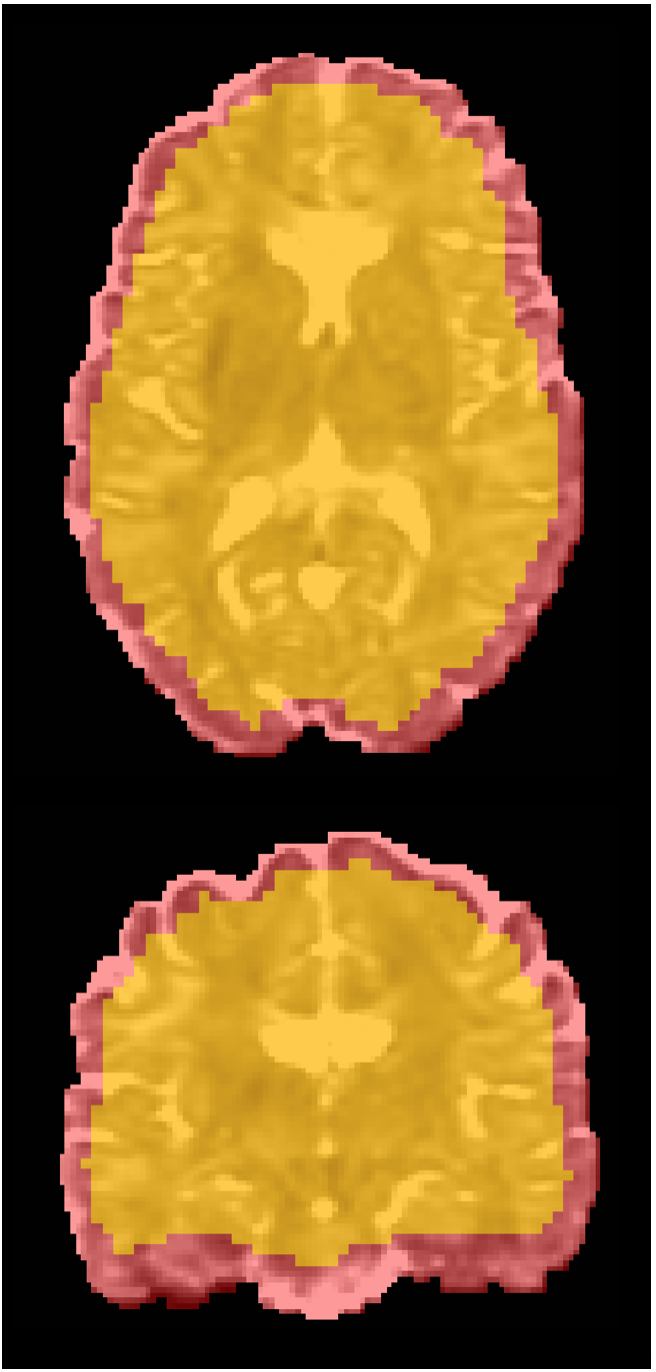
\includegraphics[width=2.75cm]{chapter_3/figures/fig_3_2.png}
	\small
	\caption{Visualisation of ``interior'' (yellow) and ``exterior'' regions (red). The interior region consists of a set of patches contained entirely within the brain while the exterior region consists of partial patches that contain mixtures of brain and background voxels} 
	\label{fig:mask}
	%\vspace{- 15pt}
\end{figure}

Table~\ref{tab:compare_1} shows that our baseline achieves $8.5\%/39.8\%$ reduction in RMSE for the super-resolution of DTIs on the HCP dataset on the interior/exterior regions with respect to the best published method, BIQT-RF\cite{tanno2016bayesian}. While the standard deviations are higher, the improvements are more pronounced in MAP-MRI super-resolution, reducing the average RMSEs by $49.6\%$ and $63.5\%$ on the interior and exterior regions. We note that that IQT-RF and BIQT-RF are only trained on interior patches, and super-resolution on boundary patches requires a separate \textit{ad hoc} procedure. Despite including exterior patches in training our model, which complicates the learning task, the baseline CNN out-performs the RF methods on both regions. We see similar improvements in the out-of-distribution Lifespan dataset.

Reconstruction is faster than the RF baselines; the 3D-ESPCN is capable of estimating the whole high-resolution DTI/MAP-MRI under 10/60 seconds on a CPU and $1/10$ second(s) on a GPU. On the other hand, BIQT-RF takes $\sim10$ mins with 8 trees on both DTIs and MAP-MRIs. The fully convolutional architecture of the model enables to process input patches of different size from that of training inputs, and we achieve faster reconstruction by using larger input patches of dimension $25^3\cdot c$ where $c$ is the number of channels. We also note that the reconstruction time of the variational dropout based models increases by a factor of the number of MC samples used at test time, although it is possible, with more memory, to leverage GPU parallelisation by making multiple copies of each input patch and treating them as a mini-batch. On the other hand, the heteroscedastic CNN enjoys the same inference speed of the baseline since only the mean network is used for reconstruction (the covariance network is only employed to quantify the estimated intrinsic uncertainty). 

\begin{table}
	\center
	\footnotesize
	\begin{tabular}{@{}lclclclcl}
		\hline
		Models & HCP (interior) & HCP (exterior)& Life (interior) & Life (exterior)   \\ 
		\hline	
		CSpline-interpolation & $10.069 \pm$ n/a & $31.738\pm$ n/a & $32.483\pm$ n/a & $49.066\pm$ n/a  \\
		$\beta$-Spline interpolation& $9.578\pm$ n/a  & $98.169\pm$ n/a &$33.429\pm$ n/a &$186.049\pm$ n/a   \\
		IQT-RF & $ 6.974 \pm 0.024$  & $23.139\pm0.351$ & $10.038\pm0.019$&$25.166\pm0.328$   \\ 
		BIQT-RF & $6.972 \pm 0.069$  &$23.110\pm0.362$  & $9.926\pm0.055$ &$25.208\pm0.290$ \\
		\hline 
		3D-ESPCN(baseline)                      & $6.212\pm0.017$    & $13.609\pm0.084$  &$8.902\pm0.020$   &$16.389\pm0.114$\\
		+ Binary Dropout ($p=0.1$)           & $6.319 \pm 0.015$  & $13.738\pm0.048$   &$9.093\pm0.024$  &$16.489\pm0.099$ \\
		+ Gaussian Dropout ($p=0.05$)     & $6.463\pm0.034$    & $14.168\pm0.051$  &$9.184\pm0.048$  & $16.653\pm0.092$\\
		
		+ Variational Dropout (I)                  & $6.194\pm0.013$    & \cellcolor{red!15} $\mathbf{13.412\pm 0.041}$   &$8.874\pm0.027$  &  \cellcolor{red!15} $\mathbf{16.147\pm0.051}$ \\
		+ Variational Dropout (II)                 & $6.201\pm0.015$    & \cellcolor{blue!15}  $13.479\pm0.047$   & $8.878\pm0.031$  &\cellcolor{blue!15} $16.230\pm0.075$ \\
		
		+ Hetero.                                        & $6.135\pm0.029 $   & $15.469\pm 0.231$  & $8.885\pm0.041$ & $17.208\pm0.211$ \\
		
		+ Hetero. + Variational Dropout (I)   & \cellcolor{blue!15} $6.121\pm0.015$    &$13.591\pm0.051$   & \cellcolor{red!15} $\mathbf{8.837\pm0.043}$ &$16.261\pm0.053$\\ 
		+ Hetero. + Variational Dropout (II)  & \cellcolor{red!15} $\mathbf{6.116\pm0.013}$   &$13.622\pm0.099$   & \cellcolor{blue!15} $8.861\pm0.031$  &$16.387\pm0.098$\\
% The previous experiment with 8 train subjects
%		3D-ESPCN(baseline)                   & $6.378\pm0.015$   & $13.909\pm0.071$   &  $8.998\pm0.021$   &$16.779\pm0.109$\\
%	   	+ Binary Dropout ($p=0.1$)        & $6.519 \pm 0.015$ & $14.038\pm0.038$    & $9.183\pm0.024$   &$16.890\pm0.097$ \\
%		+ Gaussian Dropout ($p=0.05$) & $6.963\pm0.034$   & $14.568\pm0.068$    & $9.784\pm0.048$   &$17.357\pm0.091$\\
%		+ Variational Dropout (I)& $6.354\pm0.015$ & \cellcolor{red!15} $\mathbf{13.824\pm 0.031}$ &$8.973\pm0.024$&\cellcolor{red!15}$\mathbf{16.633\pm0.053}$ \\
%		+ Variational Dropout (II) & $6.356\pm0.008$ & \cellcolor{blue!15} $13.846\pm0.017$  & $8.982\pm0.024$ &\cellcolor{blue!15}$16.738\pm0.073$ & \\
%		+ Hetero.  &$6.294\pm0.029 $ & $15.569\pm 0.273$  & $8.985\pm0.051$ & $17.716\pm0.277$ \\
%		+ Hetero. + Variational Dropout (I) &\cellcolor{blue!15} $6.291\pm0.012$&$13.906\pm0.048$ & \cellcolor{red!15}$\mathbf{8.944\pm0.044}$ &$16.761\pm0.047$\\ 
%		+ Hetero. + Variational Dropout (II) &\cellcolor{red!15} $\mathbf{6.287\pm0.029}$&$13.927\pm0.093$&\cellcolor{blue!15} $8.955\pm0.029$&$16.844\pm0.109$\\
		\hline
	\end{tabular}%	
	\vspace{-1mm}
\caption{Super-resolution results on diffusion tensor images (DTIs) of HCP and Lifespan datasets for different upsampling methods. For each method, an ensemble of $10$ models are trained on different training sets generated by randomly extracting a set of patch pairs from the common $16$ HCP subjects. For each model, the average RMSE ($\times 10^{-4} \text{mm}^2/\text{s} $) over subjects in respective datasets is first computed and the mean/std of such average RMSE over the ensemble are then reported. Best results in bold red, and the second best in blue. }
\label{tab:compare_1}	
\end{table}

\begin{table}
	\center
	\footnotesize
	\begin{tabular}{@{}lclclclcl}
		\hline
		Models & HCP (interior) & HCP (exterior)& Life (interior) & Life (exterior)   \\ 
		\hline	
		CSpline interpolation& $5.234 \pm$ n/a & $30.362\pm$ n/a & $7.135\pm$ n/a & $29.232\pm$ n/a  \\
		$\beta$-Spline interpolation &  $4.852 \pm$ n/a  &  $63.446\pm$ n/a & $6.523\pm$ n/a &  $56.937\pm$ n/a \\
		IQT-RF \cite{alexander2017image}&   $4.538 \pm 0.113$& $25.541\pm0.131$  & $5.882\pm0.121$  & $26.137\pm0.279$   \\ 
		BIQT-RF \cite{tanno2016bayesian} & $4.838 \pm 0.129$  &$25.523\pm0.175$  & $5.949\pm0.131$ &$27.509\pm0.233$ \\
				
		\hline
		3D-ESPCN(baseline)  & $2.285 \pm0.126$   & $9.316\pm0.127$ & $4.195 \pm0.163$ & $11.922 \pm0.192$ \\
		+ Binary Dropout ($p=0.1$) &    $2.283 \pm0.154$	 & $9.272\pm0.132$ & $4.120 \pm0.178$ &	$11.652 \pm0.204$	\\
		+ Gaussian Dropout ($p=0.1$)  &    $2.370 \pm0.155$	& 	$9.335\pm0.144$	& 	$4.327\pm0.157$	&	$11.907 \pm0.211$	\\
		+ Variational Dropout (I)& $2.155\pm0.122$ &   $9.205\pm0.193$ 	& 	$3.997 \pm0.153$  & $11.547 \pm0.177$ 	\\
		+ Variational Dropout (II)& $2.172\pm0.128$ &  $9.112\pm0.173$  &  $3.972 \pm0.132$ &  $11.511 \pm0.172$ & \\
		+ Hetero. &$1.998\pm0.132 $ & $11.294\pm 0.216$  & $3.872 \pm0.140$   & $12.084 \pm0.129$\\
		+ Hetero + Variational Dropout (I) &\cellcolor{red!15} $\textbf{1.951} \pm \textbf{0.122}$ & \cellcolor{blue!15}$9.102\pm0.181$ & \cellcolor{red!15} $\textbf{3.572}\pm\textbf{0.171}$  &\cellcolor{red!15}$\textbf{11.037} \pm\textbf{0.192}$  \\ 
		+ Hetero + Variational Dropout (II)&\cellcolor{blue!15} $1.969 \pm 0.119$ &\cellcolor{red!15}$\textbf{9.052}\pm\textbf{0.162}$& \cellcolor{blue!15} $3.606 \pm0.141$ & \cellcolor{blue!15}$11.311 \pm0.195$  \\
		\hline
		3D-ESPCN(without outlier removal)  & $3.425 \pm0.163$   & $13.284\pm0.239$ & $6.032 \pm0.229$ & $15.5 13 \pm0.273$ \\
		+ Hetero. &$2.264\pm0.153 $ & $11.306\pm 0.172$  & $3.919 \pm0.140$   & $12.821 \pm0.150$\\
		+ Hetero + Variational Dropout (I) & $2.138 \pm0.159$ & $10.022\pm0.187$ &  $3.681\pm0.193$  &$12.133 \pm 0.205 $  \\ 
		+ Hetero + Variational Dropout (II)& $2.133 \pm 0.188$ & $ 9.988 \pm 0.209$&  $3.690 \pm0.184$ & $12.052 \pm0.212$  \\
		\hline
	
	\end{tabular}%	
\vspace{-1mm}
\caption{Super-resolution results on MAP-MRIs of HCP and Lifespan datasets for different upsampling methods. For each method, an ensemble of $5$ models are trained on different training sets generated by randomly extracting a set of patch pairs from the common $16$ HCP subjects. For each model, the average RMSE over subjects in respective datasets is first computed and the mean/std of such average RMSEs over the ensemble are then reported. Best results in bold red, and the second best in blue. In addition, the performance of 3D-ESPCN and its probabilistic variants trained on data without outlier removal are also included.}
\label{tab:compare_2}
\end{table}


% Table for 8 training subjects 
%\begin{figure}[t]
%	%\vspace{- 15pt}
%	\centering
%	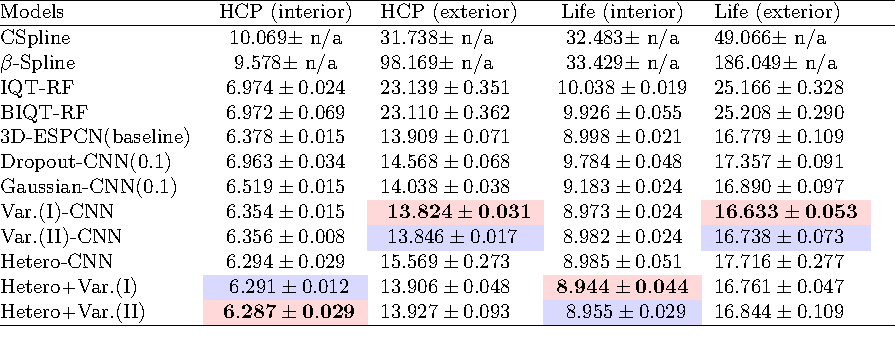
\includegraphics[width=\linewidth]{chapter_3/figures/table_1_3.pdf}\label{fig:performance_compare}
%	\small
%	\caption{(a) RMSE on HCP and Lifespan dataset for different upsampling methods. For each method, an ensemble of $10$ models are trained on different training sets, and the mean/std of the average errors over $8$ test subjects are computed over the ensemble. Best results in bold red, and the second best in blue. (b) Interior (yellow) and exterior region (red).} 
%	%\vspace{- 15pt}
%\end{figure}

Table~\ref{tab:compare_1} shows that, on both HCP and Lifespan data, modelling both intrinsic and parameter uncertainty (i.e. Hetero. + Variational Dropout (I), (II)) achieves the best reconstruction accuracy in DTI super-resolution. We observe that modelling intrinsic uncertainty with the heteroscedastic network on its own further reduces the average RMSE of the baseline 3D-ESPCN on the interior region with high statistical significance ($p<10^{-3}$). However, poorer performance is observed on the exterior than the baseline. On the other hand, using $200$ MC weight samples, we see modelling parameter uncertainty with variational dropout (see Variational Dropout.(I)-CNN) performs best on both datasets on the exterior region. Combination of heteroscedastic model and variational dropout (i.e. Hetero. + Variational Dropout (I) or (II)) leads to the top 2 performance on both datasets on the interior region and reduces errors on the exterior to the level comparable or better than the baseline. 

%Table ~\ref{tab:compare_1} shows that, on both HCP and Lifespan data, the heteroscedastic network further reduces the average RMSE of the baseline 3D-ESPCN on DTI super-resolution on the interior region with high statistical significance ($p<10^{-3}$). However, poorer performance is observed on the exterior than the baseline. Using $200$ MC weight samples, we see Var.(I)-CNN performs best on both datasets on the exterior region. Combination of heteroscedastic model and variational dropout (i.e. Hetero+Var.(I) or (II)) leads to the top 2 performance on both datasets on the interior region and reduces errors on the exterior to the level comparable or better than the baseline. 

Similarly, Table~\ref{tab:compare_2} shows that the best performance in MAP-MRI super-resolution comes from the combined models (i.e. Hetero.+Variational Dropout.(I) and (II)). We observe that as with the DTI case,  modelling intrinsic uncertainty through the heteroscedastic network improves the reconstruction accuracy on the interior region, whilst the errors on the exterior are increased with respect to the baseline 3D-ESPCN. Moreover, the improvement is pronounced when the outliers due to model fitting errors are not removed in the training data. In this case, we see that the reconstruction accuracy of 3D-ESPCN dramatrically decreases, whilst in contrast it is only marginally compromised when equipped with the heteroscedastic noise model, displaying robustness to outliers. Lastly, we note that the top-2 accuracy are consistently achieved by the joint modelling of intrinsic and parameter uncertainty (i.e. Hetero.+Variational Dropout.(I) and (II)) on both the interior and exterior regions on both HCP and Lifespan datasets.  

%Table~\ref{tab:compare_2} compares the similar results for MAP-MRI super-resolution. We observe that as with the DTI case,  the heteroscedastic network improves the reconstruction accuracy on the interior region, whilst the errors on the exterior are increased with respect to the baseline 3D-ESPCN. However, when the outliers due to model fitting errors are not removed in the training data, the reconstruction accuracy of 3D-ESPCN dramatrically decreases, whereas it is only marginally compromised when equipped with the heteroscedastic noise model. Notably, the top-2 accuracy are achieved by the combined models (i.e. Hetero+Var.(I) and Hetero+Var.(II)) on both the interior and exterior regions on both HCP and Lifespan datasets. 

The performance difference of heteroscedastic network between the interior and the exterior region roots from the loss function. The Mahalanobis term $\mathcal{M}_{\theta}(\mathcal{D})$ in eq.\eqref{eq:loss_hetero} imposes a larger penalty on the regions with smaller intrinsic uncertainty. The network therefore allocates less of its resources towards the regions with higher uncertainty (e.g. boundary regions) where the statistical mapping from the low-resolution to high-resolution space is more ambiguous, and biases the model to fit the regions with lower uncertainty. However, we note that the performance of the heteroscedastic network is still considerably better than the standard interpolation and RF-based methods. By augmenting the model with variational dropout, the exterior error of the heteroscedastic model is dramatically reduced, indicating its regularisation effect against overfitting to low-uncertainty areas. We also observe concomitant performance improvement on the interior regions on both datasets, which additionally shows the benefits of such regularisation even in low-uncertainty areas. 

Both Table~\ref{tab:compare_1} and Table~\ref{tab:compare_2} show that the use of variational dropout attains lower errors than the models with fixed dropout probabilities $p$, namely, Binary and Gaussian dropout \cite{srivastava2014dropout}. Different instances of both dropout models are trained for a range of $p$ by linearly increasing on the interval $[0.05,0.3]$ with increment $0.05$, and the test errors for the configurations with smallest RMSE on the validation set are reported in Table~\ref{tab:compare_1} and Table~\ref{tab:compare_2}. As with variational dropout models, $200$ MC samples are used for inference. In all cases, two variants of variational dropout (I) and (II) outperform the networks with the best binary or Gaussian dropout models, showing the benefits of learning dropout probabilities $p$ rather than fixing them in advance. 

\subsection{Tractography with MAP-MRI}
Reconstruction accuracy does not necessarily reflect real world utility. We thus further assessed the benefits of super-resolution with a tractography experiment on the Prisma dataset, which contains two DWIs of the same subject at two different image resolutions---1.35 mm and 2.5 mm isotropic voxels, as detailed in Sec.~\ref{sec:dataset}. An ensemble of $10$ best performing CNN (3D-ESPCN+Hetero.+Variational Dropout(I)) is used to super-resolve the MAP-MRI coefficients \cite{ozarslan2013mean} derived from the low-resolution DWIs, and the ensemble predictions aggregated into the final output by taking the average estimate weighted by the inverse of the estimated intrinsic uncertainty. Lastly, the high-resolution multi-shell DWIs are obtained from this super-resolved MAP volume. Specifically, the Spherical Mean Technique (SMT) is used to fit a microscopic tensor model to the predicted dataset \cite{kaden2016quantitative}. The voxel-by-voxel estimated model parameters inform the spatially varying fibre response function that is used to recover the fibre orientation distribution through spherical deconvolution. Afterwards, we perform probabilistic tractography \cite{tournier2010improved} with the fibre pathways randomly seeded in the brain. In a similiar fashion, we also generate high-resolution datasets by using IQT-RF and linear interpolation.

%(Ryu): Reconstruction accuracy does not reflect real world utility, thus we further assessed the benefits of super-resolution with a downstream tractography experiment on the Prisma dataset, which contains two DWIs of the same subject from a Siemens Prisma 3T scanner, at two different image resolutions (1.35 mm and 2.5 mm isotropic voxels). The full details of the dataset are available in Sec.~\ref{sec:dataset}. An ensemble of $8$ 3D-ESPCN+Hetero.+Variational Dropout(I) is used to super-resolve the MAP-MRI coefficients \cite{ozarslan2013mean} derived from the low-resolution DWIs (2.5 mm), and the ensemble predictions aggregated into the final output by taking the average estimate weighted by the inverse of the estimated intrisic uncertainty. Lastly, the high-res DWIs (1.25 mm) are obtained from this super-resolved MAP volume. In a similiar fashion, we also generate high-res datasets by using IQT-RF and linear interpolation.

\begin{figure}[ht]
	\vspace{3mm}
	\centering
	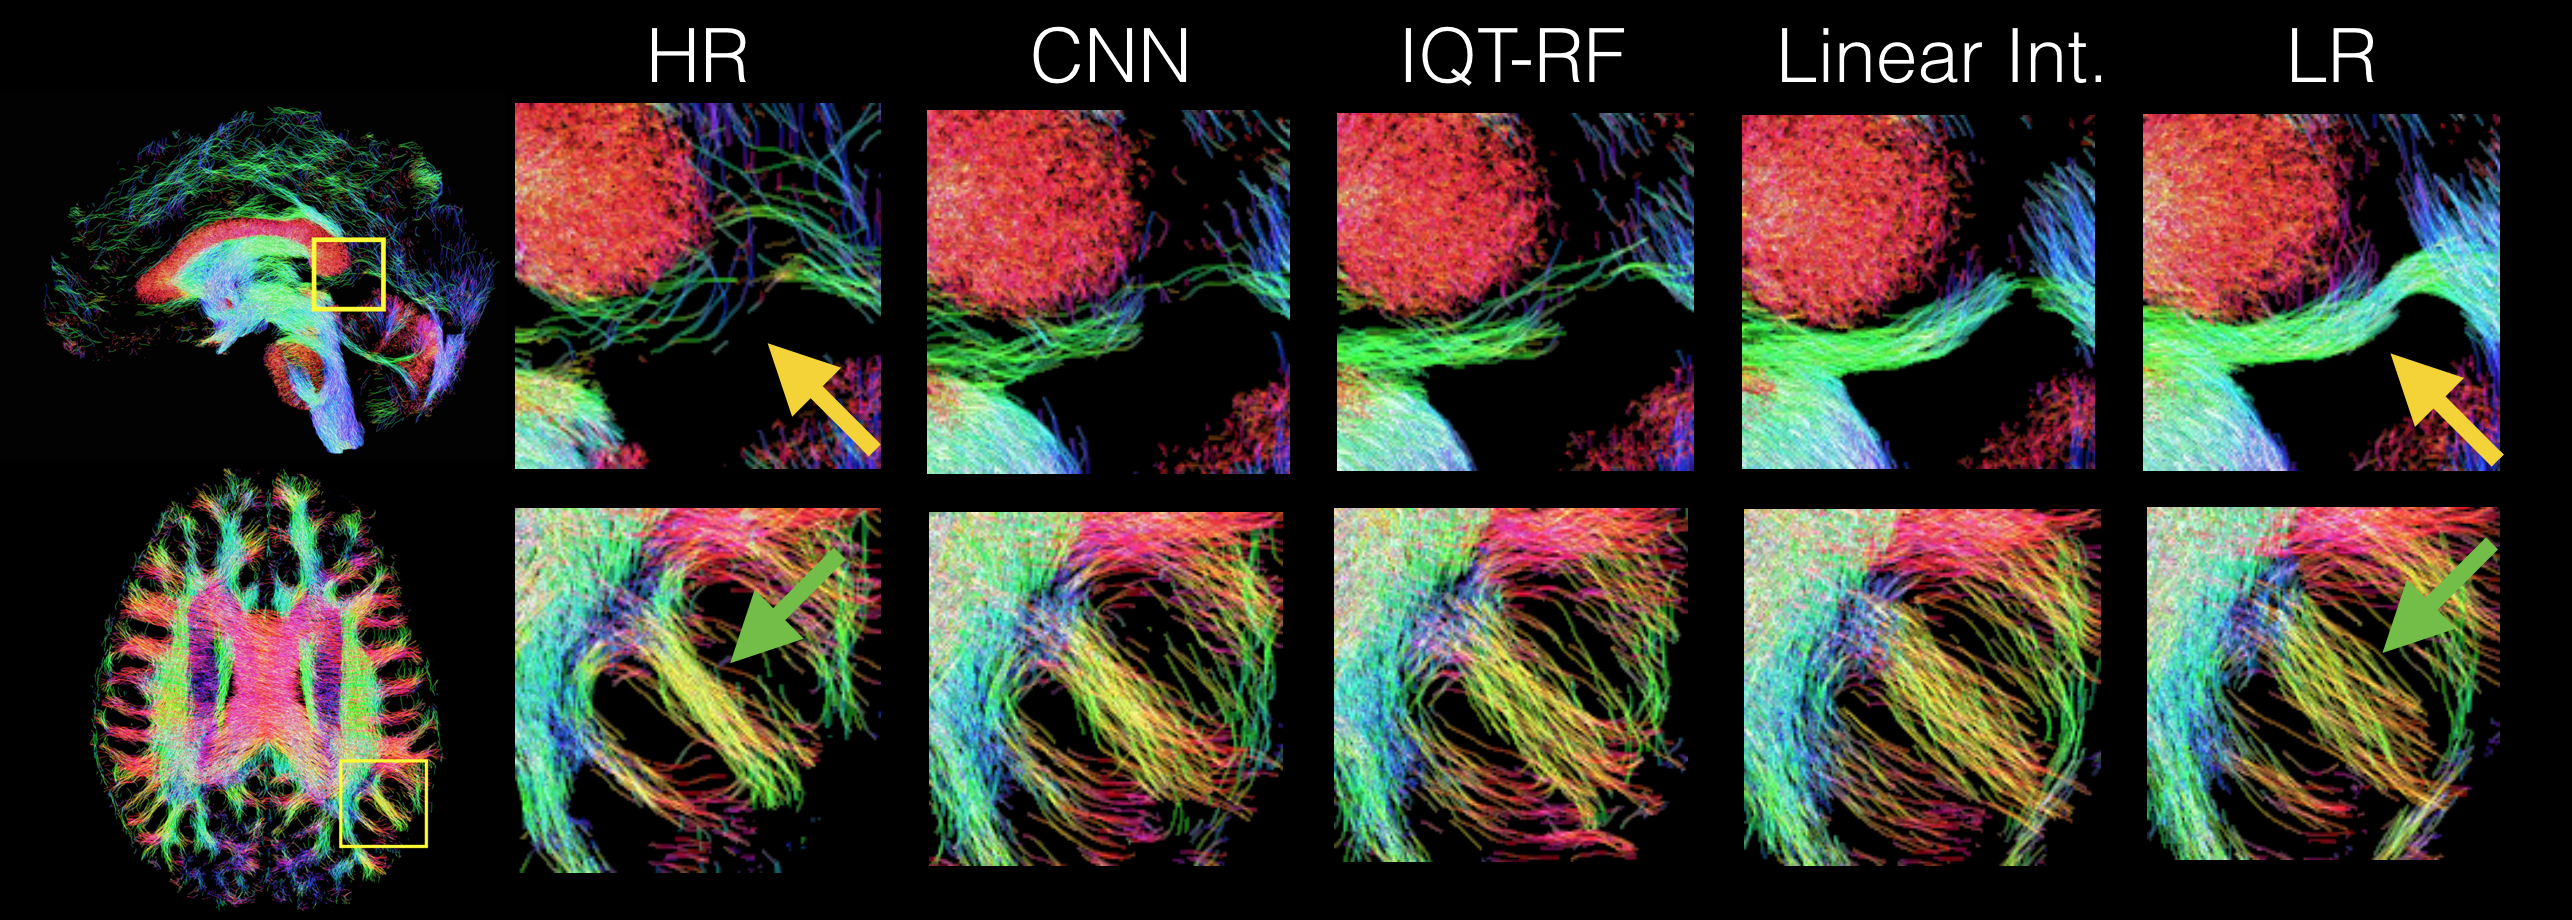
\includegraphics[width=\linewidth]{chapter_3/figures/figure_7_5.png}\label{fig:uncertainty_map}
	\small
	\caption{Streamline maps of the probabilistic tractography \cite{tournier2010improved} applied on Prisma dataset for different upsampling methods and visualised with MRtrix3 \cite{tournier2012mrtrix}. From left to right: (i) High-res acquisition, (ii) CNN (3D-ESPCN+Hetero.+Variational Dropout(I)) prediction; (iii) Random Forest IQT \cite{alexander2017image}; (iv) Linear interpolation; (v) Low-res acquisition. The yellow arrows in the top row indicate the location of a false positive tract detected in the low-resolution acquisition, whilst the green arrows in the bottom row show an example white matter tract, which is more sharply reconstructed at high resolution. } 
	\label{fig:tract}
	%	\vspace{-1em}
\end{figure}

\clearpage
Fig.~\ref{fig:tract} shows that IQT via our best performing CNN makes a tangible difference in downstream tractography. In the top row, tractography on the low-resolution data produces a false-positive tract under the corpus callosum (yellow arrow), which tractography at high resolution avoids. Reconstructured high-resolution images from IQT-RF and CNN predictions avoid the false positive better than linear interpolation. Note that we do not expect to reproduce the high-resolution tractography map exactly, as the high-resolution and low-resolution images are not aligned exactly and the high-resolution and prediction have different resolutions (1.35 mm vs. 1.25 mm). The bottom row shows sharper recovery of small gyral white matter pathways (green arrow) at high-resolution than low-resolution resulting from reduced partial volume effect. CNN reconstruction produces a sharper pathway than RF-IQT and linear interpolation, more closely reflecting the high-resolution tractography.
%In the top row, tractography on the low-resolution data indicates presence of a false-positive tract under the corpus callosum (yellow arrows) while not picked up in the high-resolution data. Both IQT-RF and CNN predictions appear less sensitive to false indication tracts in the input compared to linear interpolation. Also, the bundle structures close to the outer boundary (green arrow) gracefully becomes shaper moving right to left. This is consistent with the CNN-based improvements on the exterior region for DTI-SR.

\subsection{Uncertainty Quantification}
%\textcolor{red}{Need to sharpen the preamble to better motivate the experiments we perform if necessary. Or we could remove this and motivate better at the start of the respective subsections \ref{sec:uncertainty_HCP} and \ref{sec:unseen_abnormality}.}
 In this section, we investigate the value of uncertainty modelling in enhancing the safety of super-resolution system beyond reduced reconstruction errors. Firstly, in Sec.~\ref{sec:uncertainty_HCP}, we study the utility of predictive uncertainty map as a proxy measure of reconstruction accuracy on healthy test subjects from both HCP and Lifespan datasets. Secondly, in Sec.~\ref{sec:unseen_abnormality}, we look into the behaviour of uncertainty maps in the presence of abnormal features that are not present in the training data. 

% In particular, we aim to demonstrate that the proposed uncertainty quantification method not only provides a subject-specific and spatially varying metric of output reliability, but also adds a high-level transparency to the predictive performance by decoupling the sources of predictive uncertainty. 

%In this section, we aim to display the value of uncertainty modelling beyond performance imrovement. In particular, we demonstrate quantification of uncertainty not only provides a safer means to deploy the super-resolution system, but also adds a high-level transparency to the predictive performance through decoupling the sources of uncertainty. 

\subsubsection{Healthy Test Subjects} \label{sec:uncertainty_HCP}
We employ the most performant CNN model (3D-ESPCN + Hetero. + Variational Dropout(I)) to generate the high-resolution predictions of \textit{mean diffusivity} (MD) and \textit{fractional anisotropy} (FA), and their associated predictive uncertainty maps.  Here we draw $200$ samples of high-resolution DTI predictions for each subject from the predictive distribution $q_\phi^*(\mathbf{y}|\mathbf{x})$, and then the FA and MD maps of each prediction are computed. The sample mean and standard deviation are then calculated from these samples to generate the final estimates of high-resolution MD/FA maps and their corresponding predictive uncertainty. 

Fig.~\ref{fig:uncertainty_map} displays high correspondence between the error (RMSE) maps and the predictive uncertainty on both FA and MD of a HCP test subject. This demonstrates the potential utility of uncertainty map as a surrogate measure of prediction accuracy. In particular, the MD uncertainty map captures subtle variations within the white matter and the cerebrospinal fluid (CSF) at the centre. Also, in accordance with the low reconstruction accuracy, high predictive uncertainty is observed in the CSF in MD. This is expected since the CSF is essentially free water with low signal-to-noise-ratio (SNR) and is also affected by biological noise such as cardiac pulsations. The reconstruction errors are high in FA prediction on the bottom-right quarter of the brain boundary, close to the skull, which is also reflected in the uncertainty map. 

%We measure the MC expectation and variance of \textit{mean diffusivity} (MD) and \textit{fractional anisotropy} (FA) with respect to the predictive distribution $q_\phi^*(\mathbf{y}|\mathbf{x})$ of 3D-ESPCN+ Hetero.+Variational Dropout(I) by MC sampling. Comparative results are shown in Fig.4, where we drew $200$ samples of high-resolution DTIs from the predictive distribution of the Hetero+Var.(I) and the FA and MD maps of each are computed. The uncertainty map is highly correlated with the error maps. In particular, the MD uncertainty map captures subtle variations within the white matter and central CSF, which demonstrates the potential utility of the uncertainty map as a surrogate measure of accuracy.


%Here we show that uncertainty over the estimated high-resolution DTI volume $I_{high-resolution}$ can be propagated to any functions of interest $M(I_{high-resolution})$ through MC-estimation. Specifically, Fig.\ref{fig:uncertainty_map} shows the uncertainty maps (standard deviation) over \textit{mean diffusivity} (MD) and \textit{fractional anisotropy} (FA) along with the predictions, the ground truth images and the corresponding errors (RMSE). We sequentially estimated the mean and standard deviation over FA and MD by drawing $200$ samples of high-resolution DTIs from the predictive distribution of the heteroscedastic network and computing both measures for each of them. The uncertainty map displays a high degree of correspondence with the error maps. In particular, the MD uncertainty map captures subtle variations within the white matter and even in the central CSF. 
%For example, in present-day clinical neurology, various brain pathologies may be best detected by looking at particular measures of anisotropy and diffusivity. 
%\begin{figure}[ht]
%	%\vspace{-2em}
%	\centering
%	\subfigure[Uncertainty propagation]{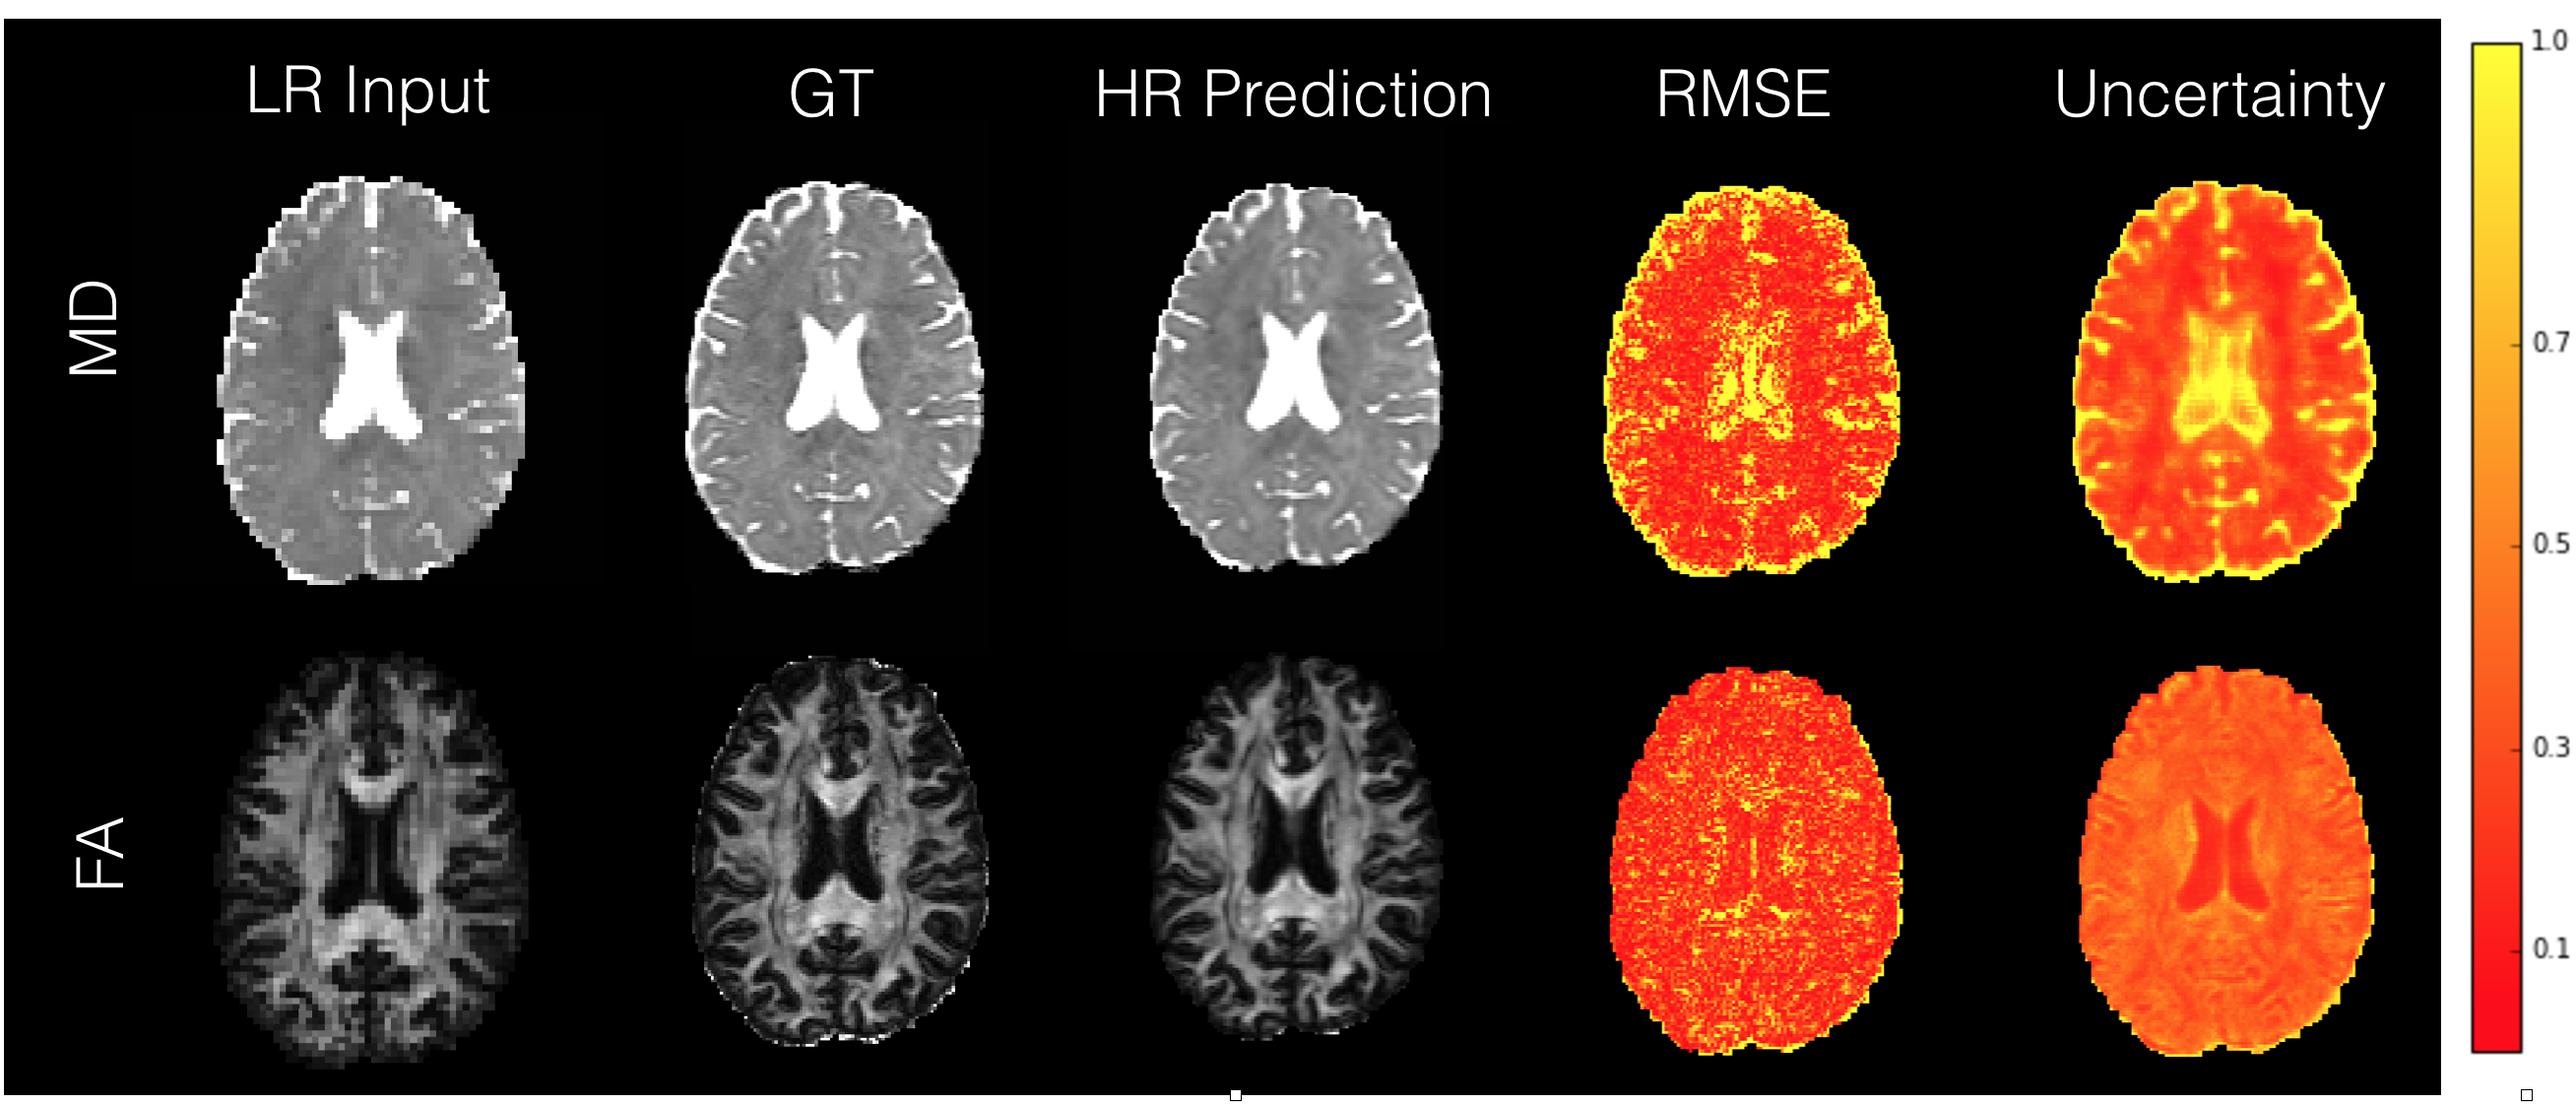
\includegraphics[width=13cm]{chapter_3/figures/fig_4_2.png}\label{fig:uncertainty_map}}
%	\subfigure[Tumour]{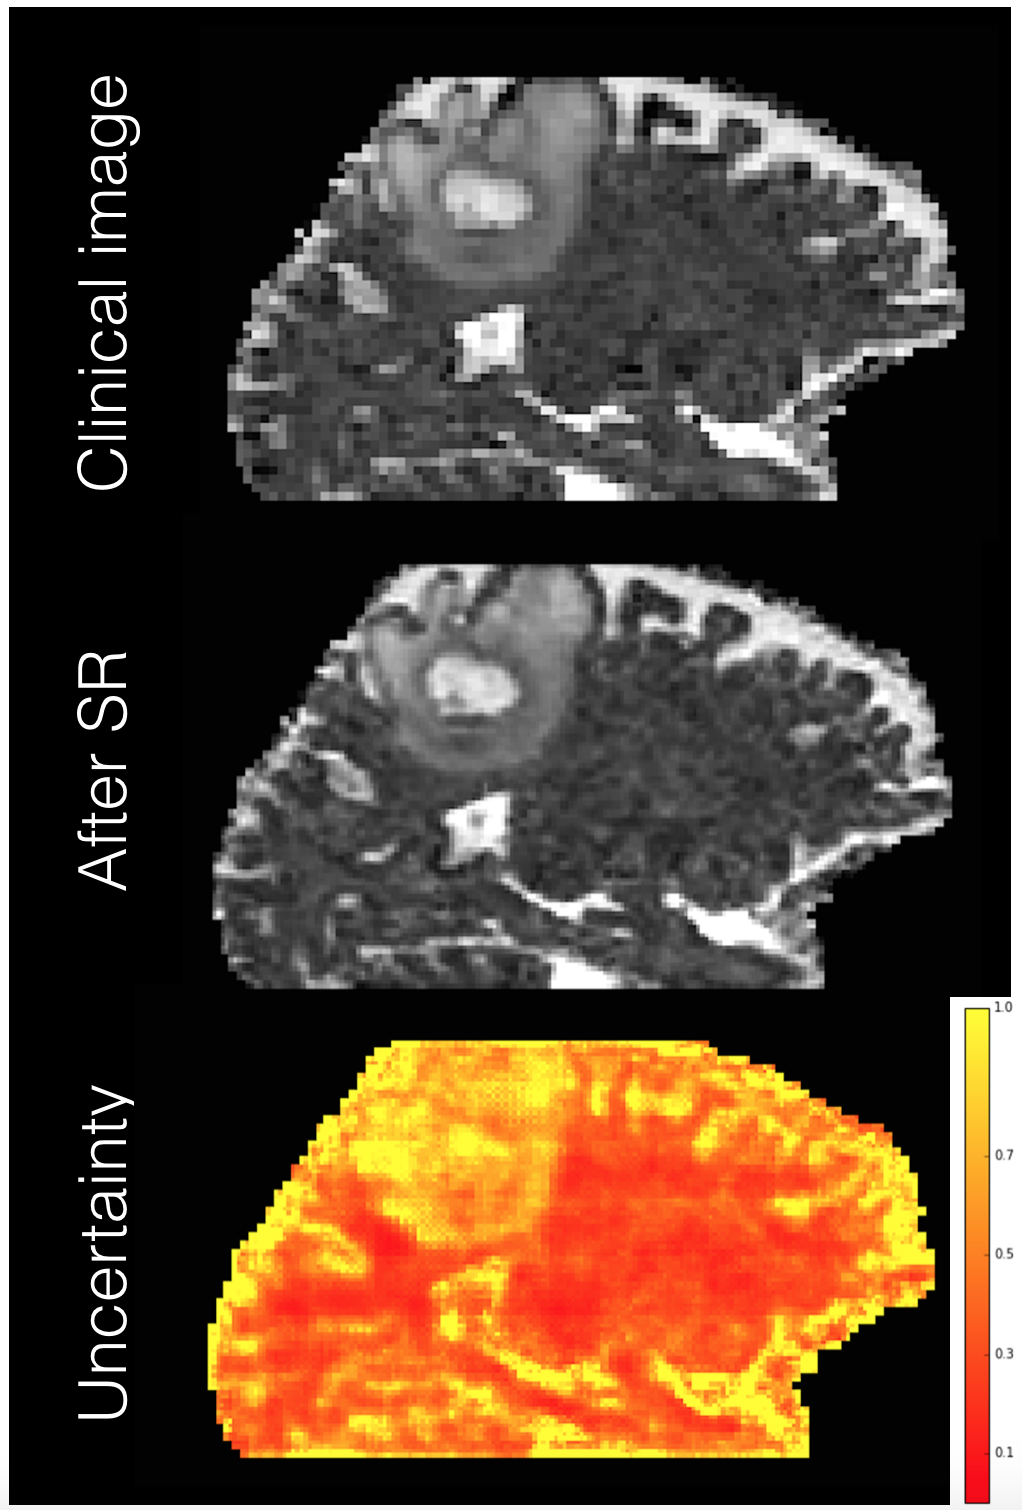
\includegraphics[width=3.7cm]{chapter_3/figures/fig_6_2.png}\label{fig:tumour}}
%	\small
%	\caption{(a) Comparison between RMSE and uncertainty maps for FA and MD computed on a HCP subject. low-resolution input, ground truth and high-resolution prediction are also shown. (b) DTI SR on a brain tumour patient. From top to bottom: (i) MD computed from the original DTI; (ii) the estimated high-resolution version; (iii) uncertainty.} 
%	%	\vspace{-1em}
%\end{figure}
\begin{figure}[t]
	%\vspace{-2em}
	
	\centering
	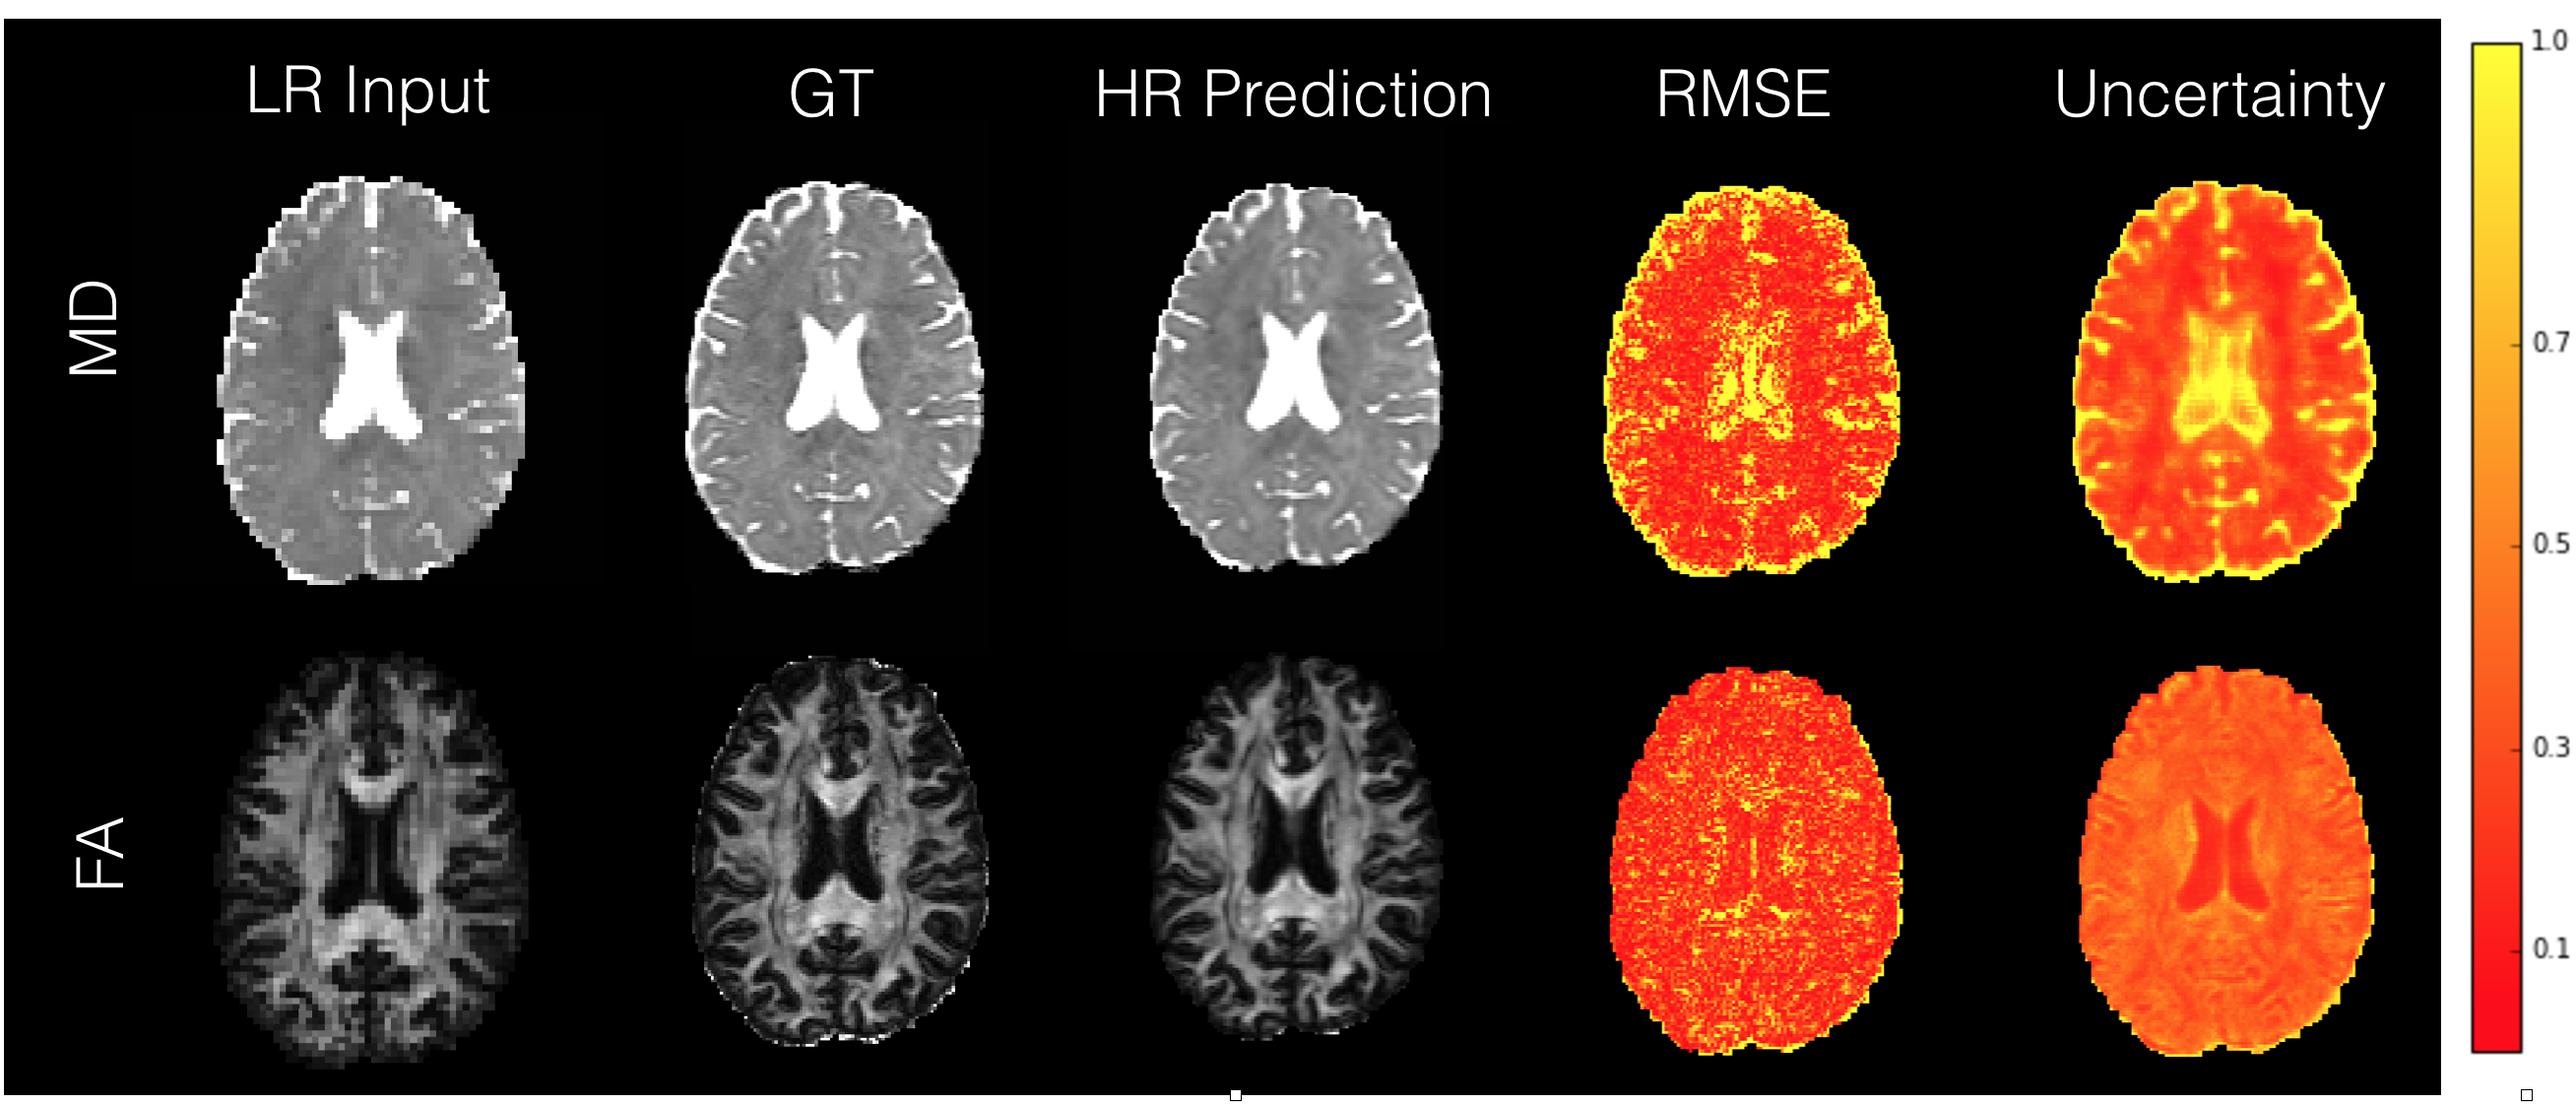
\includegraphics[width=\linewidth]{chapter_3/figures/fig_4_2.png}
	\small
	\caption{Comparison between voxel-wise RMSE and predictive uncertainty maps for FA and MD computed on a HCP test subject (min-max normalised for MD and FA separately). Low-res input, ground truth and the mean of high-resolution predictions are also shown.} 
	\label{fig:uncertainty_map}
	%	\vspace{-1em}
\end{figure}

Fig.~\ref{fig:roc} tests the utility of predictive uncertainty map in discriminating potential predictive failures in the predicted high-resolution MD map. We define ground truth ``safe'' voxels as the ones with reconstruction error (RMSE) smaller than a fixed value, and the task is to separate them from the remaining ground-truth ``risky'' voxels  by thresholding on their predictive uncertainty values. The threhold for defining safe voxels is set to $1.5\times10^{-4} \text{ s/mm}^2$, such that the risky voxels mostly concentrate on the outer-boundary and the CSF regions (which account for $17.5\%$ of all voxels under consideration). Here the positive class is defined as ``safe'' while  the negative class is defined as ``risky''. Fig.~\ref{fig:roc} (a) shows the corresponding receiver operating characteristic (ROC) curve of such binary classification task, which plots the true-positive-rate (TPR) against the false-positive-rate (FSR) computed based on all the voxels in the 16 HCP training subjects. In this case, TPR decribes the percentage of correctly detected safe voxels out of all the safe ones, while FPR is defined as the percentage of risky voxels that are wrongly classified as safe out of all the risky voxels. We then select the best threshold by maximising the F1 score, and use this to classify the voxels in each predicted high-resolution MD into ``safe'' and ``risky'' ones for all subjects in the test HCP dataset and the Lifespan dataset. Fig.\ref{fig:roc} (b) shows the inter-subject average of the TPR and FPR on both datasets. While on average TPR slightly worsens compared to the results on the training subjects, FPR improves in both cases---notably, this uncertainty-based classification is able to correctly identify 96\% of risky predictions on unseen subjects from out-of-training-distribution dataset, namely Lifespan, which differs in demographics and underlying acquisition. Fig.\ref{fig:roc} (c) visualises the classification results to the pre-defined ``ground truth" on one of the Lifespan subjects, which illustrates that the generated ``warning'' aggressively flags potentially risky voxels at the cost of thresholding out the safe ones. 

%We define the ‘safe’ voxels as the ones with reconstruction error (RMSE) smaller than a fixed value, and want to separate them from the rest by thresholding on their predictive uncertainty values. The threhold for defining ‘ground truth’ safe voxels is set to $1.5\times10^{-4} \text{ s/mm}^2$, such that the non-safe voxels mostly concentrate on the outer-boundary and the CSF regions (which accout for $17.5\%$ of all voxels under consideration). The receiver operating characteristic (ROC) curve of such binary classification task is then plotted based on the all the voxels in 16 of the HCP training subjects and the best threshold is chosen as the one with the maximal F1 score with the false positive rate below $10\%$ (see Fig.\ref{fig:roc} (a)). Then, this optimal threshold is used to classify the voxels in each predicted high-resolution MD into ‘safe’ (black) and ‘risky’ ones (red) for all subjects in the test HCP dataset and the Lifespan dataset. Fig.\ref{fig:roc} (b) shows the inter-subject average of the true-positive-rate (TPR) and false-positive-rate (FPR) on both datasets. While on average TPR slightly worsens, FPR improves in both cases---notably, this uncertainty-based classification is able to correctly identify 96\% of risky predictions on unseen subjects from out-of-training-distribution dataset, namely Lifespan. Fig.\ref{fig:roc} (c) visualises the classification results to the pre-defined ``ground truth" on one of the Lifespan subjects.

\begin{figure}[t] 
	\centering
	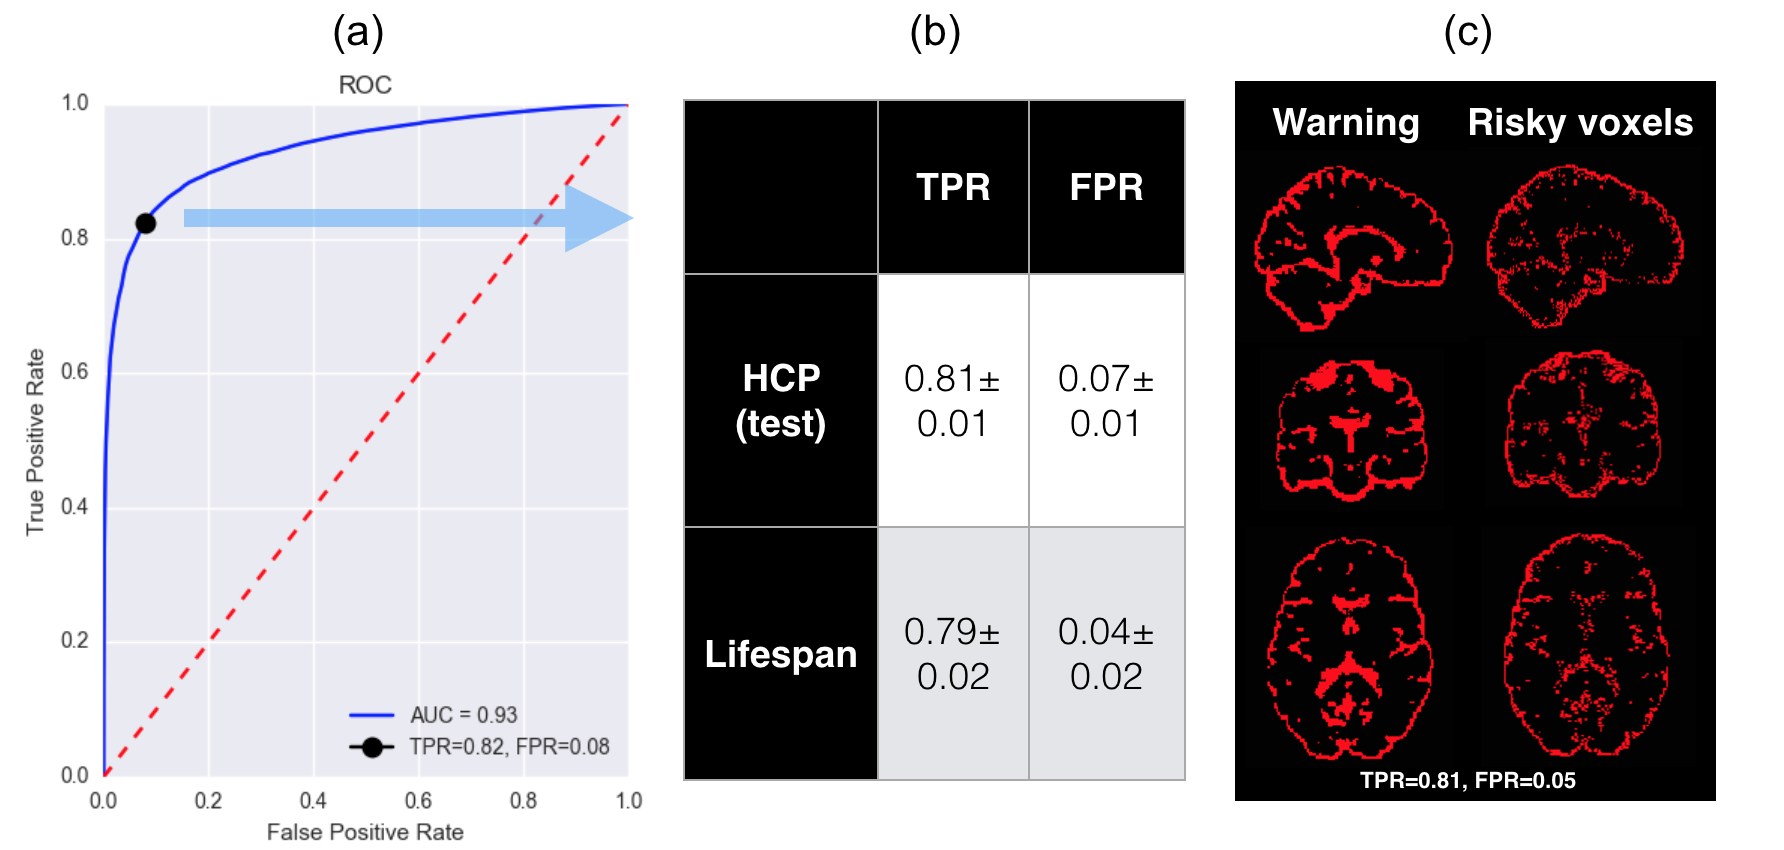
\includegraphics[width=0.9\linewidth]{chapter_3/figures/fig_5_6.png}
	\small
	\caption{Discrimination of ``safe'' voxels in the predicted high-resolution MD map by thresholding on predictive uncertainty. Here a single 3D-ESPCN + Hetro. + Variational Dropout (I) model is used to quantify the predictive uncertainty over each image volume. (a) the ROC curve plots the true positive rate (TPR) against false positive rate (FPR) computed  for a range of threshold values on the foreground voxels in the training subjects. Best threshold (black dot) was selected such that F1 score is maximised and is employed to separate ``safe'' voxels from ``risky'' ones; (b) the average TPR and FPR over the 16 test HCP subjects and the 16 Lifespan subjects are shown; (c) an example visualisation of the ``ground truth'' safe (black) and risky (red) voxels on a Lifespan subject along with the corresponding classification results denoted as ``warning''. } 
	
	
	\label{fig:roc}
\end{figure}

%In particular, we applied the best-performing SR model (Hetero+Variational (II) ESPCN) trained on a healthy HCP cohort to super-resolve the DTI of a brain tumour patient. The raw data (DWI) is processed as before, and the $b = 700 \text{ s/mm}^2$ measurement with voxel size  $2^3 \text{ mm}^3$ is used as the input. The observation and model uncertainty on the first DTI component are separately illustrated along with the input and the predicted high-resolution image. Although the ground truth is unavailable, the estimated image seems to sharpen the original image without introducing noticeable spurious features. The observation uncertainty map indicates higher uncertainty to the region of tumour than the surrounding healthy white matter as desired. Understanding the behaviours of these uncertainty measures in an `unfamiliar' test environment and their relations to predictive performance remains an important future work for designing a more generalisable method.


\subsubsection{Unseen Abnormalities and Uncertainty Decomposition} \label{sec:unseen_abnormality}
We separately visualise the propagated intrinsic and parameter uncertainty over the predicted high-resolution MD map on images of subjects with a variety of different unseen abnormal structures, such as benign cysts, tumours (Glioma) and focal lesions caused by multiple sclerosis (MS). We emphasise here that the all these images have been acquired with different protocols. Specifically, benign cysts in the HCP datasets represent abnormalities in images acquired with the same protocol as the training data, while tumours and MS lesions are examples of pathologies present in out-of-distribution imaging protocols. In all cases, we use the SR network, Hetero.+Variational Dropout (I), trained on healthy subjects from HCP dataset. For each of $200$ different sets of parameters $\{\theta_{t}\}_{t=1}^{200}$ sampled from the posterior distribution $q(\theta|\mathcal{D})$,  we draw $10$ samples of high-resolution DTIs from the likelihood, $\{\mathbf{y}^{t}_{j}\}_{j=1}^{10} \sim p(\mathbf{y}|\theta_{t},\mathbf{x},\mathcal{D})$, compute the corresponding MD, and approximate the two constituents of predictive uncertainty with the MC estimators given in eq.\eqref{eq:mc_model_uncertainty} and \eqref{eq:mc_intrinsic_uncertainty}. 

Fig.~\ref{fig:healthy_abnormal} shows the reconstruction accuracy along with the components of predictive uncertainty over the high-resolution MD map of a HCP test subject, which contains a benign abnormality (a small posterior midline arachnoid cyst). The error (RMSE) and propagated intrinsic uncertainty are plotted on the same scale whereas the propagated model uncertainty is plotted on 1/5 of the scale for clear visualisation. In this case, the predictive uncertainty is dominated by the intrinsic component. In particular, low propagated intrinsic uncertainty is observed in the interior of the cyst relative to its boundary in accordance with the high accuracy in the region. This is expected as the interior structure of a cyst is highly homogeneous with low variance in signals and the super-resolution task should therefore be relatively straightforward. On the other hand, the component of parameter uncertainty is high on the interior structure which also makes sense as such homogeneous features are underrepresented in the  training data of healthy subjects. This example illustrates how decoupling the effects of intrinsic and parameter uncertainty potentially allows one to make sense of the predictive performance. 

Fig.\ref{fig:uncertainty_decomp_1} visualises the uncertainty components generated by the same CNN model trained on datasets of varying size. We see that the propagated parameter uncertainty diminishes as the training set size increases, while the propagated intrinsic uncertainty stays more or less constant. This result is indeed what is expected as described in Fig.~\ref{fig:uncertainty_types}; the specification of network weights becomes more confident i.e. the variance of the posterior distribution decreases as the amount of training data increases, while the effect of intrinsic uncertainty is irreducible with the amount of data.  On the other hand, when the standard binary or Gaussian dropout was employed instead of variational dropout, we observed that the effect of parameter uncertainty stayed more or less constant with the size of training data. This may be a consequence of the posterior variance, largely determined by the prespecified drop-out rates, which in turn results in more static variance of predictive distribution. 

\begin{figure}[ht]
	\centering
	\begin{subfigure}{0.9\textwidth}
		\caption{HCP subject with a benign cyst}
		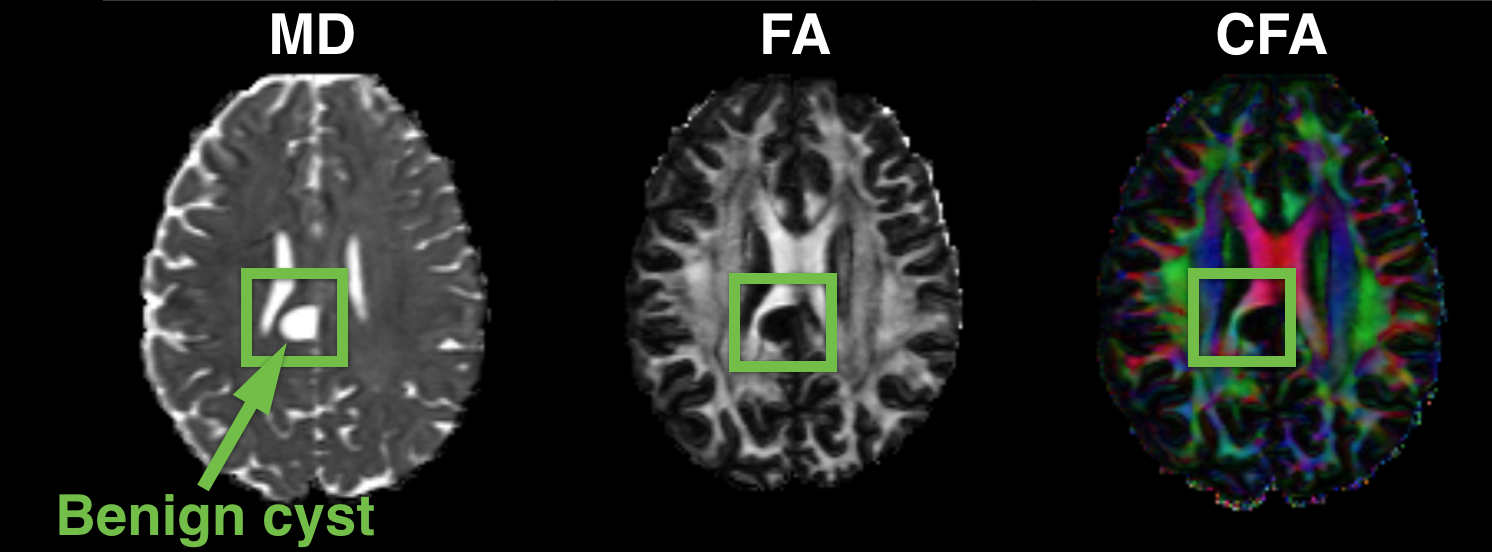
\includegraphics[width=\linewidth]{chapter_3/figures/fig_12.png}
	\end{subfigure}
	\begin{subfigure}{0.9\textwidth}
		\vspace{3mm}
		\caption{Errors vs. uncertainty components}
		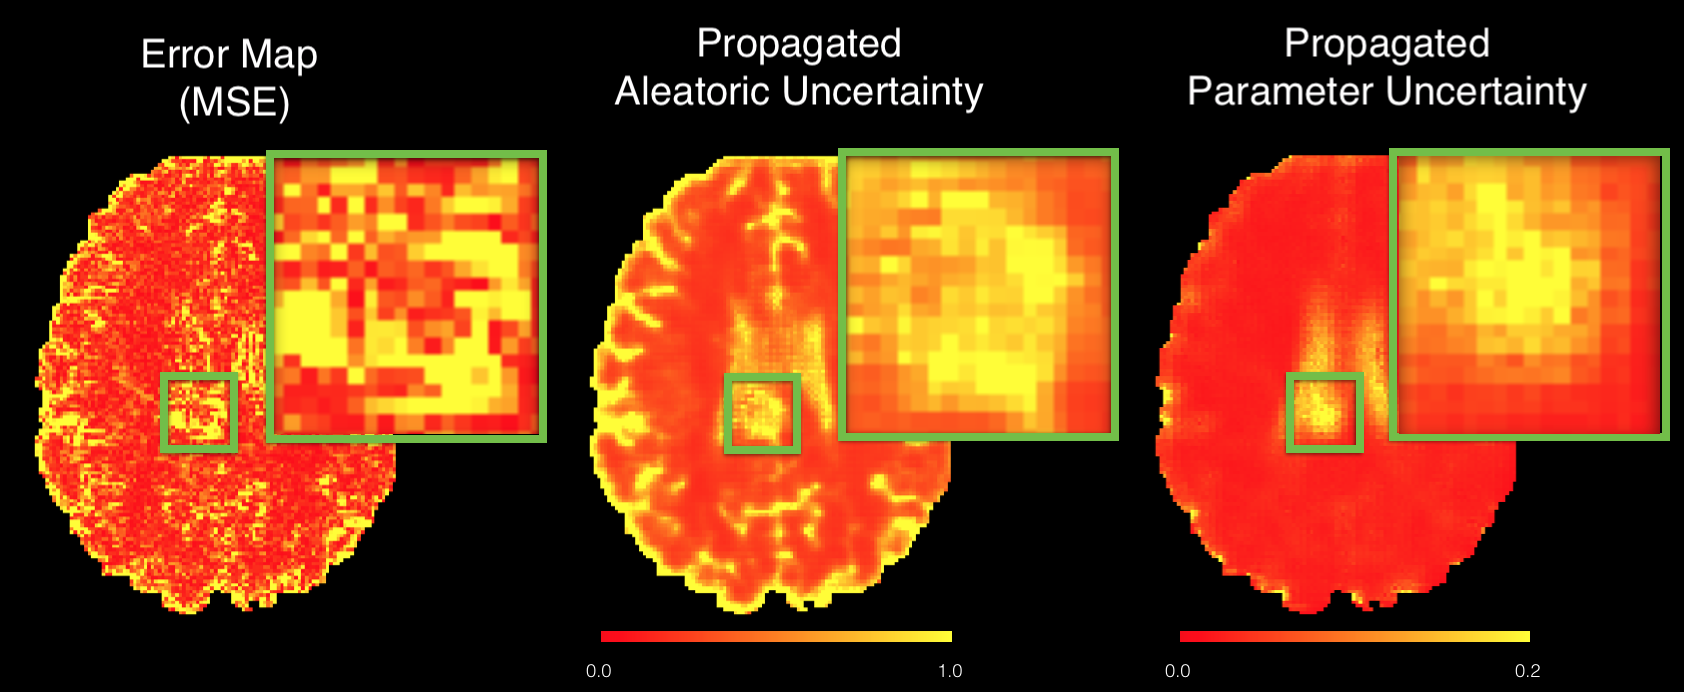
\includegraphics[width=\linewidth]{chapter_3/figures/fig_9_2.png}
	\end{subfigure}
	\caption{Visualisation of (a) MD, FA and colour FA maps computed from the DTI of a HCP subject with a small posterior midline arachnoid cyst in the central part of the brain. (b) the corresponding reconstruction accuracy (RMSE) in MD and the corresponding components of predicted uncertainty. }
	\label{fig:healthy_abnormal}
\end{figure}


%\begin{figure}[ht] 
%	\centering
%	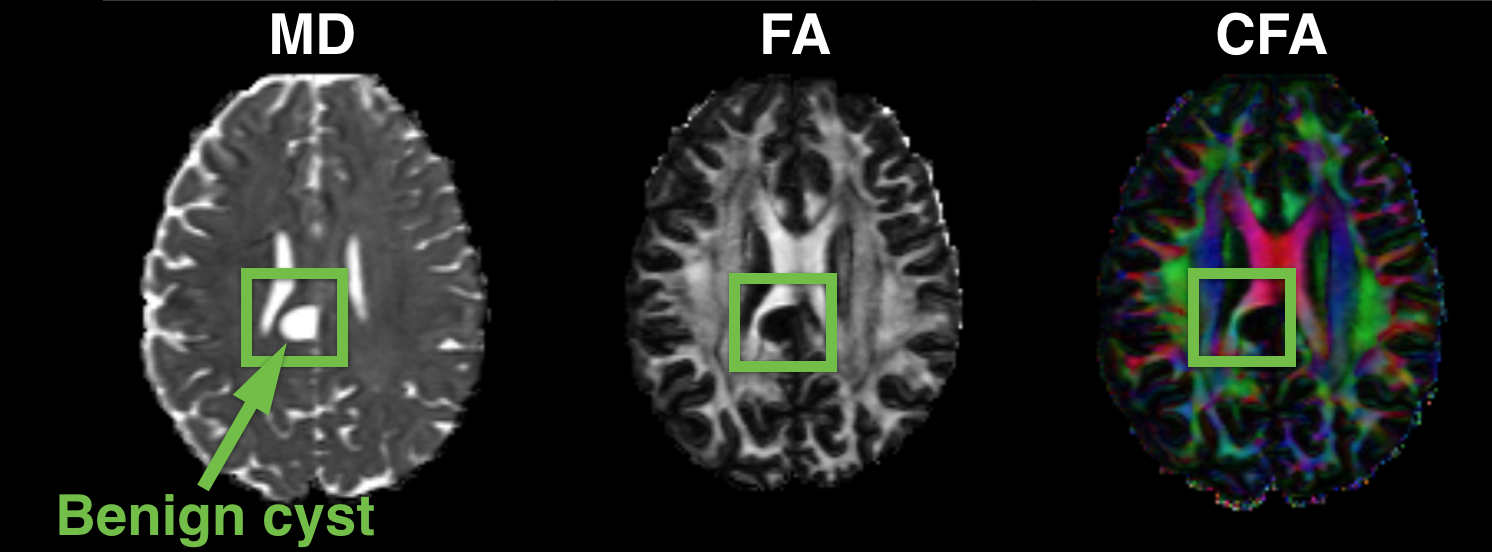
\includegraphics[width=0.65\linewidth]{chapter_3/figures/fig_12.png}
%	\small
%	\caption{MD, FA and colour FA maps computed from the DTI of a HCP subject ($105620$) with a small posterior midline  arachnoid cyst in the central part of the brain.} 
%	\label{fig:healthy_abnormal}
%\end{figure}

\begin{figure}[ht] 
	\centering
	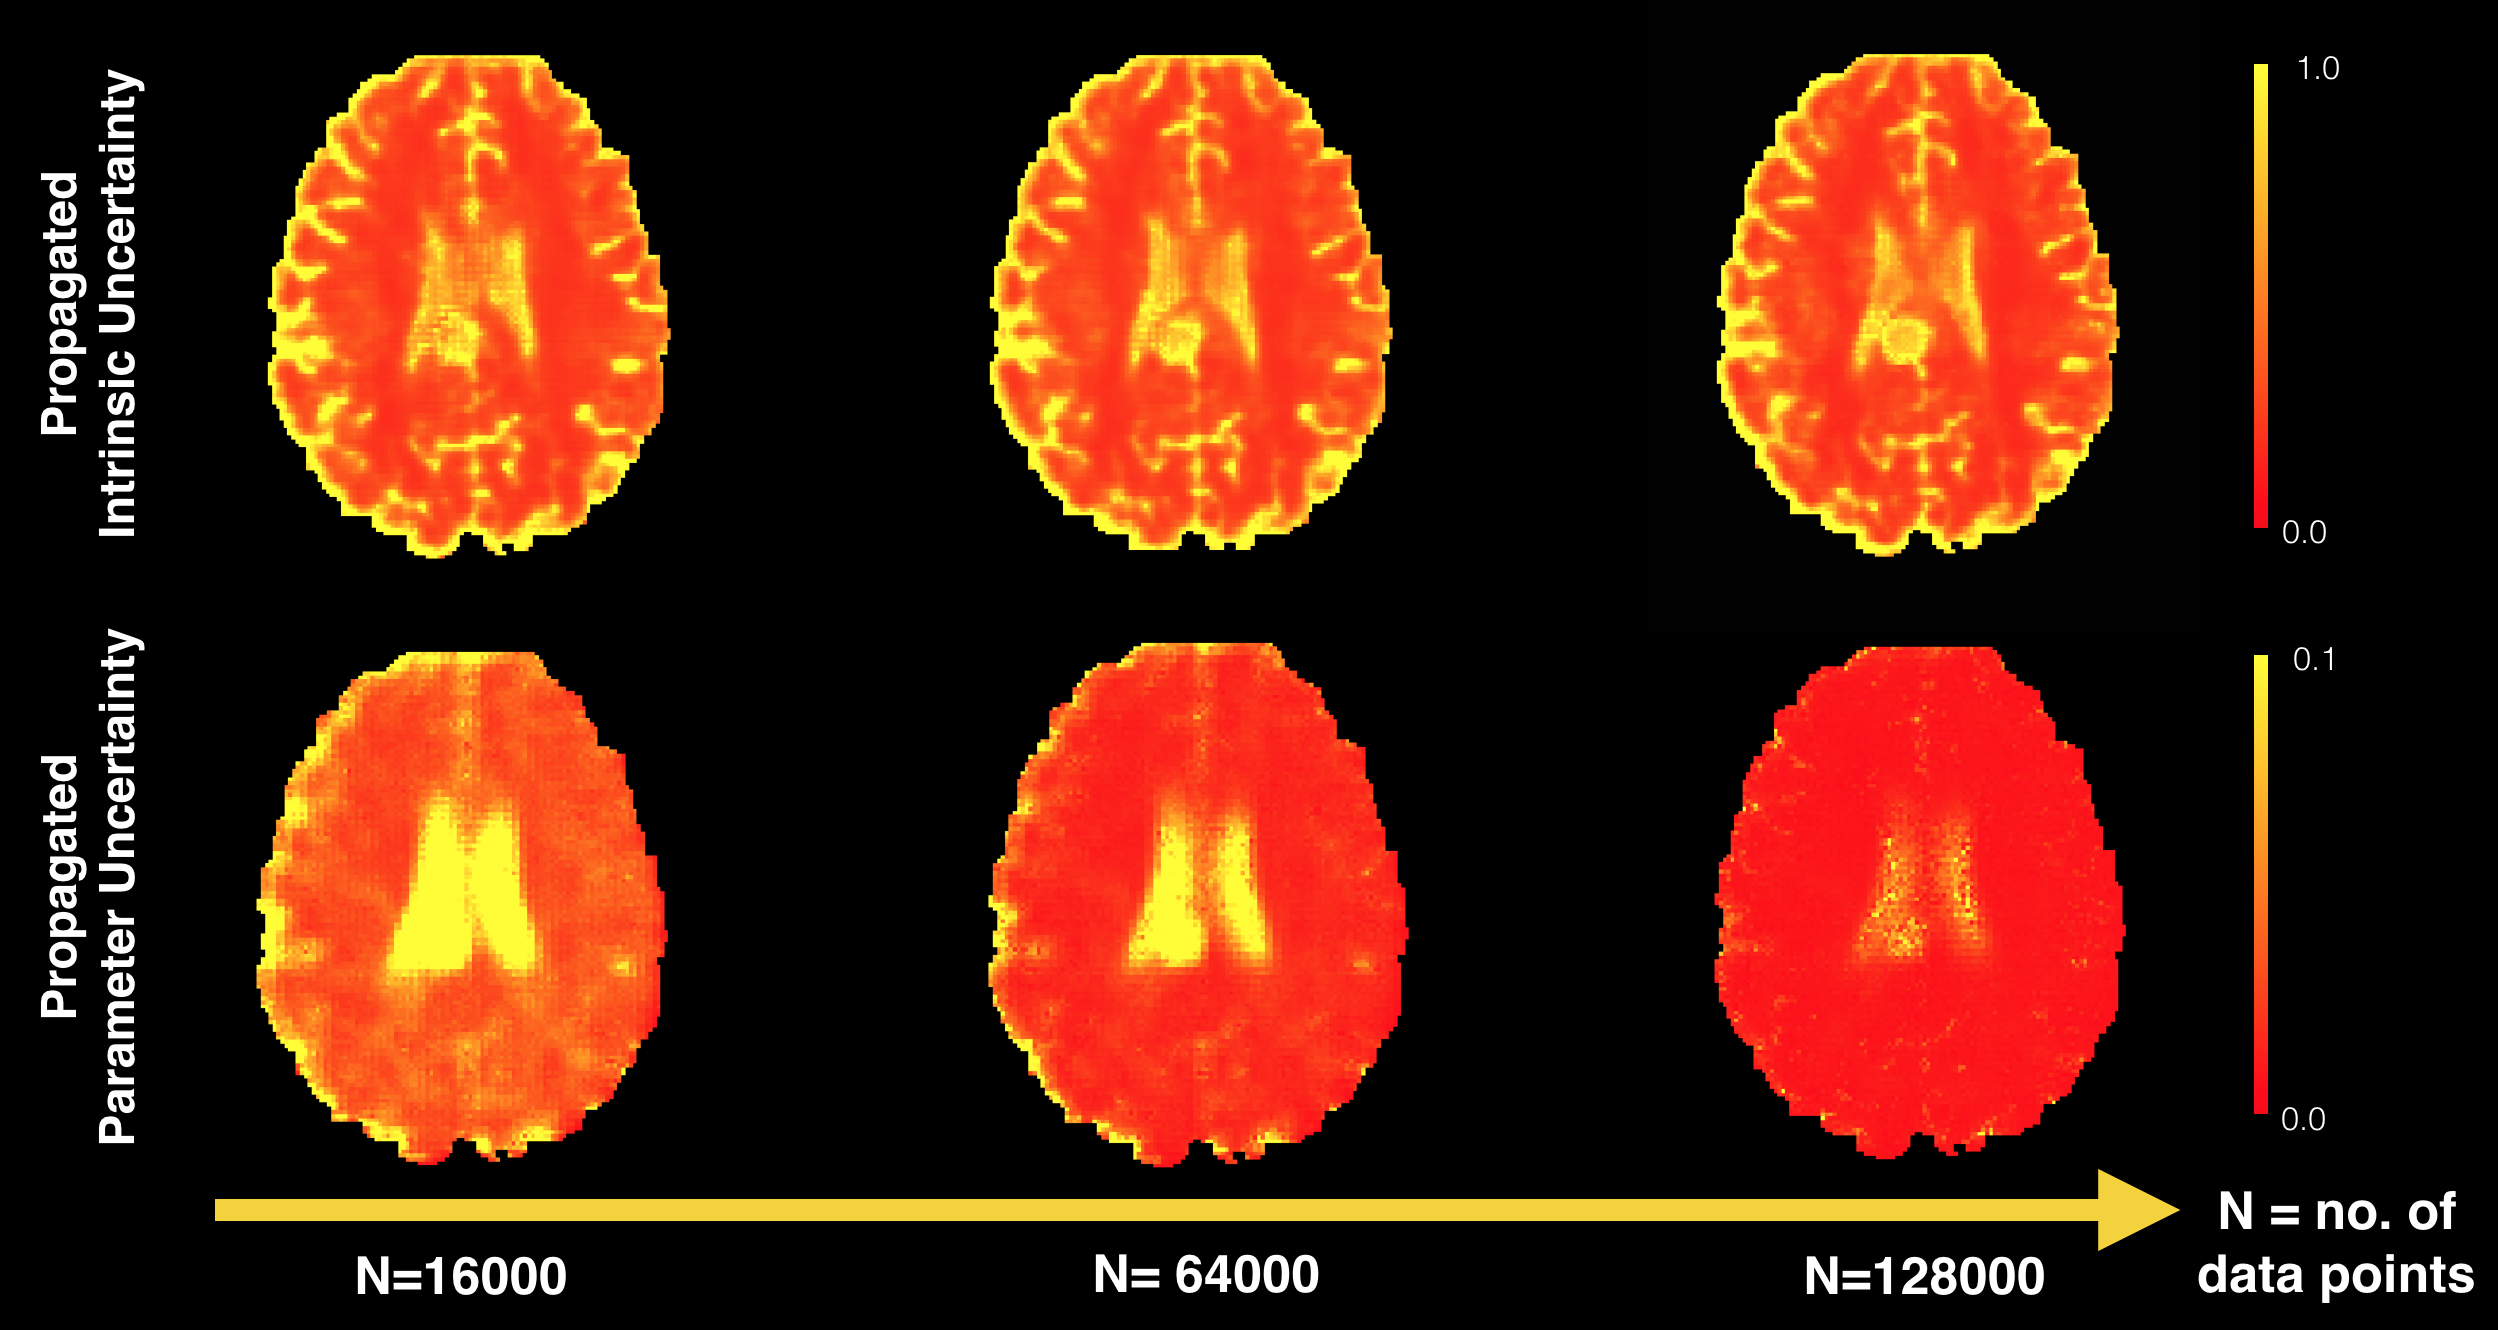
\includegraphics[width=\linewidth]{chapter_3/figures/fig_8_5.png}
	\small
	\caption{Training set size vs propagated intrinsic/parameter uncertainty on the MD map of an unseen HCP subject with a benign cyst. The uncertainty maps are normalised across all the figures. } 
	\label{fig:uncertainty_decomp_1}
\end{figure}
%
%\begin{figure}[ht] 
%	\centering
%	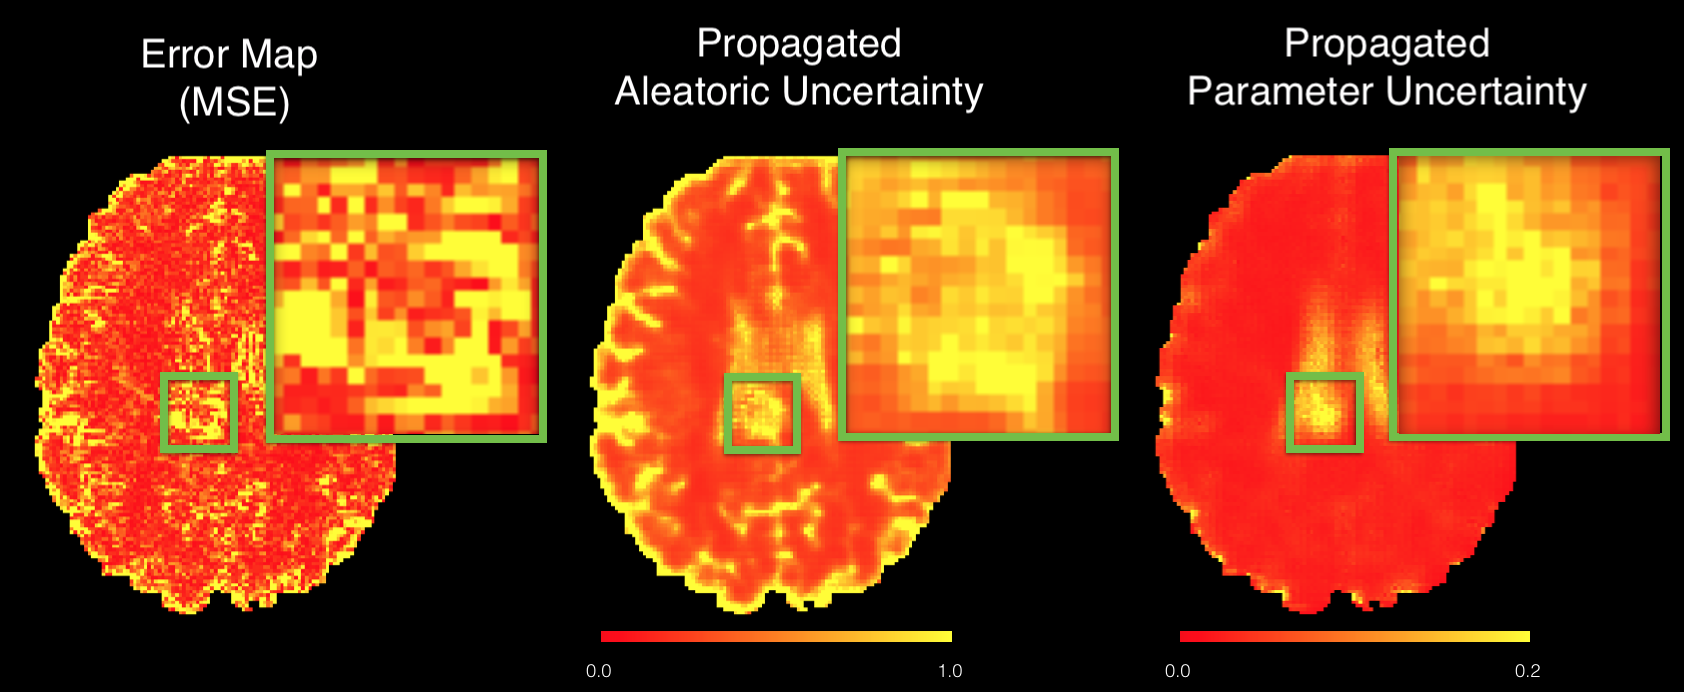
\includegraphics[width=\linewidth]{chapter_3/figures/fig_9_2.png}
%	\small
%	\caption{Comparison between reconstruction accuracy and components of predicted uncertainty on a HCP subject with a benign abnormality. } 
%	\label{fig:uncertainty_decomp_2}
%\end{figure}
\begin{figure}[ht]
	\centering
	\begin{subfigure}{\textwidth}
		\caption{Brain Tumour}
		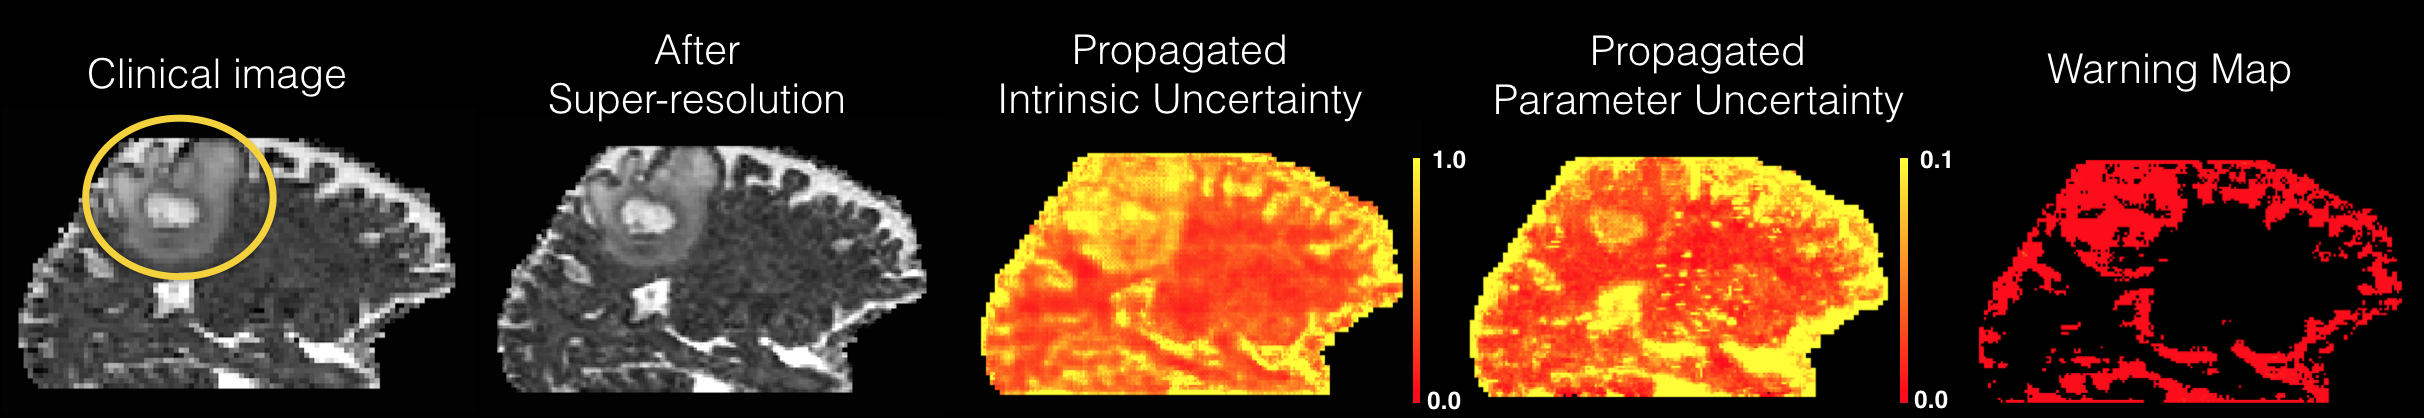
\includegraphics[width=\linewidth]{chapter_3/figures/fig_tumour_02.png}
	\end{subfigure}
	\begin{subfigure}{\textwidth}
		\vspace{2mm}
		\caption{Multiple Sclerosis}
		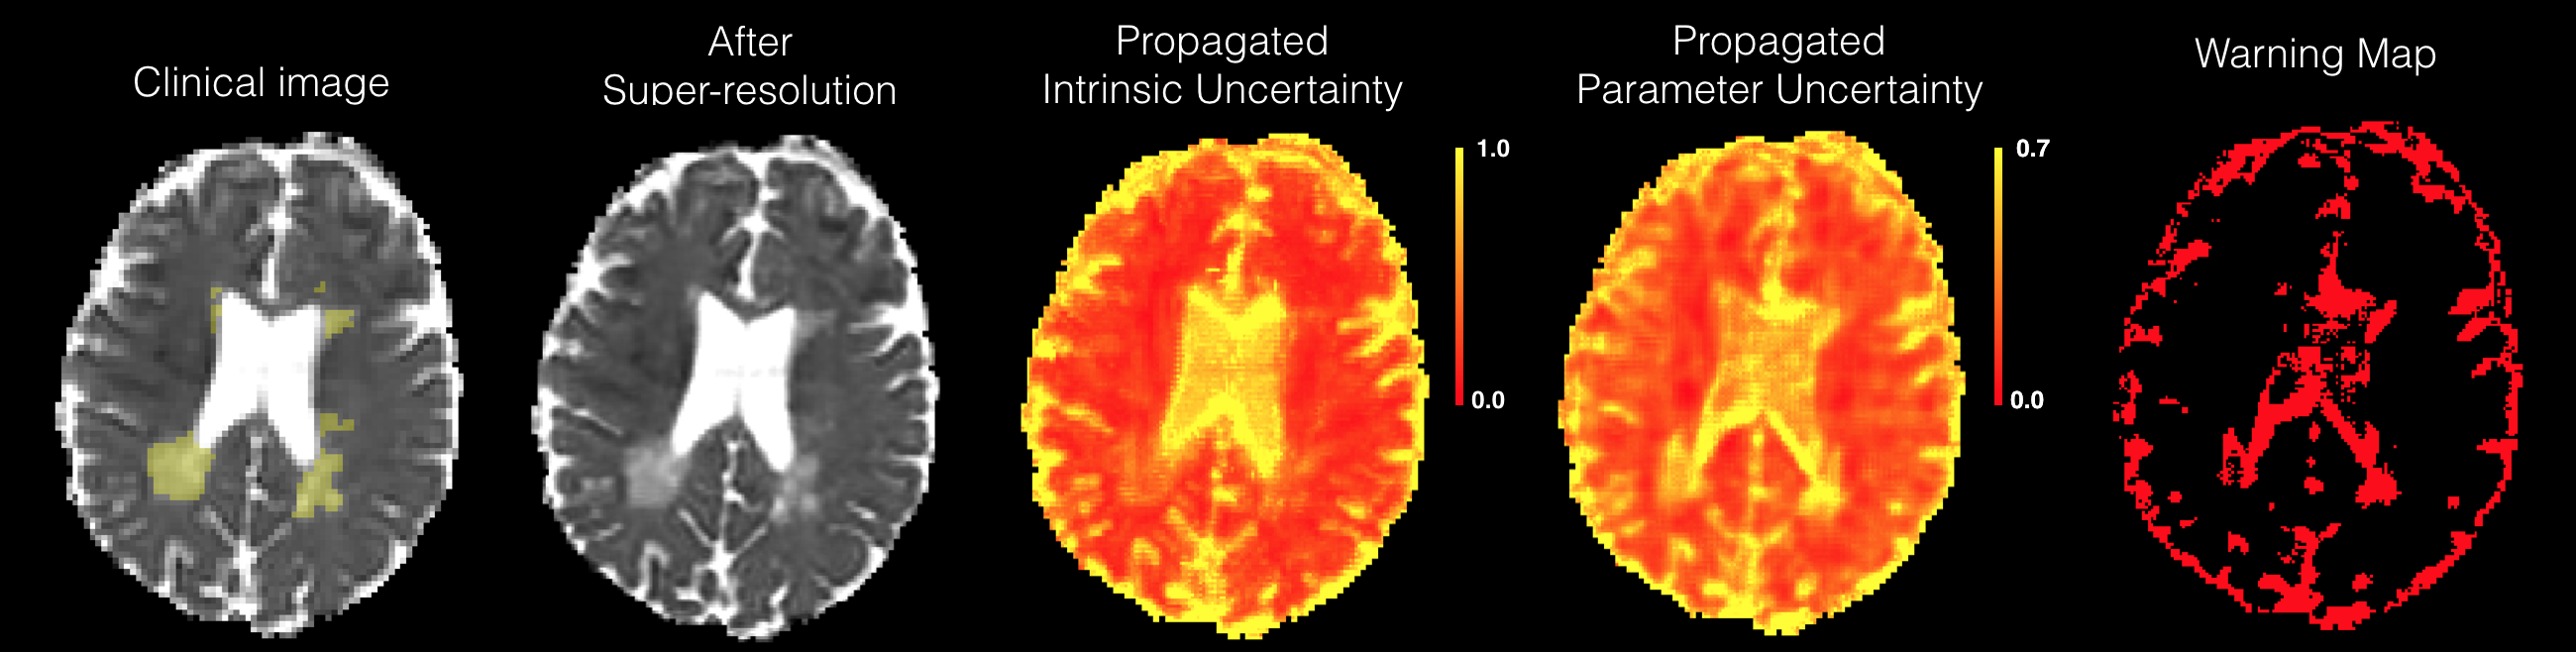
\includegraphics[width=\linewidth]{chapter_3/figures/fig_ms_03.png}
	\end{subfigure}	
	\caption{Visualisation of propagated uncertainty components on clinical images with pathology that was not present in the training data. The super-resolution is performed on the clinical images due to low-resolution, and thus the ground truths are not available in both cases. (a) shows the results on the data of a Glioma patient, and the yellow circle indicates the region of tumour. (b) shows the same set of results on a MS patient with labels of focal lesions obtained from a neurologist indicated in yellow. Each row shows from left to right: (i) MD map computed from the original DTI; (ii) MD map computed from the output of super-resolution; (iii), (iv) maps of the estimated propagated intrinsic and parameter uncertainty; (v) ``warning map'' obtained from the same threshold value used in Sec.~\ref{sec:uncertainty_HCP}, which flag large parts of the pathological features in both cases. }
	\label{fig:components_pathology}
\end{figure}

We further validate our method on clinical images with previously unseen pathologies. We note that the pathology data contain images acquired with standard clinical protocols with voxel size slightly smaller than that of the training low-resolution images and lower signal-to-noise ratio. 

%\begin{figure}[t]
%	%\vspace{-2em}
%	\centering
%	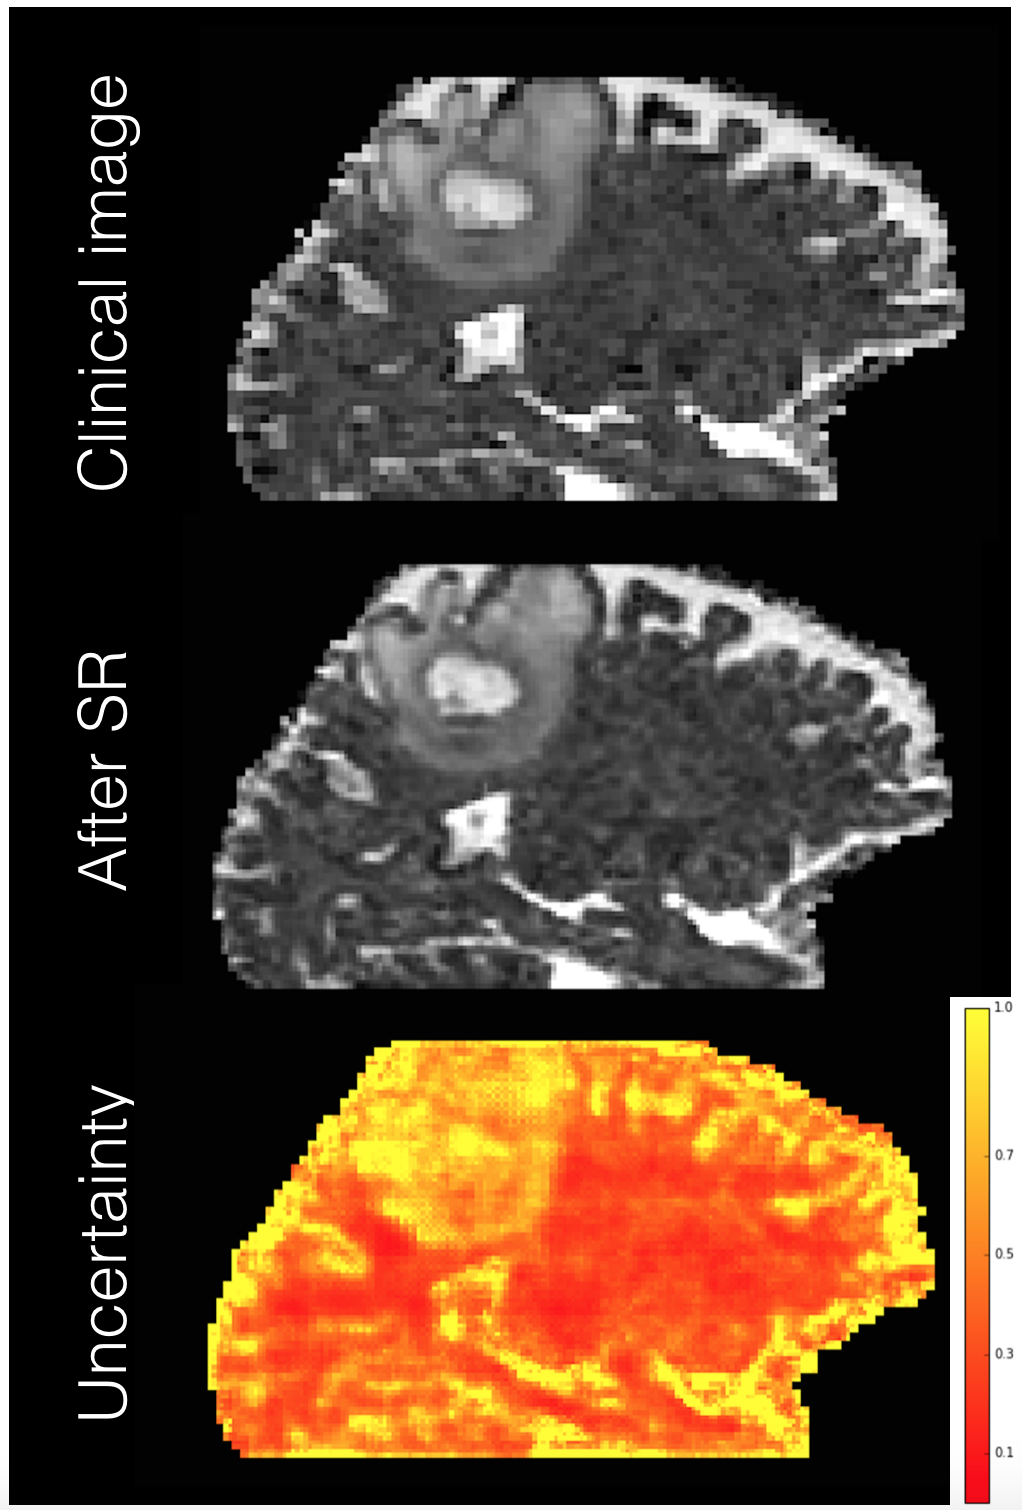
\includegraphics[width= 0.25\linewidth]{chapter_3/figures/fig_6_2.png}
%	\small
%	\caption{DTI super-resolution on the data of a brain tumour patient. From top to bottom: (i) MD computed from the original DTI; (ii) the output of super-resolution; (iii) predictive uncertainty. In total, $200$ samples are drawn from the network's predictve distribution to compute (ii) and (iii). } 
%	\label{fig:tumour}
%	%	\vspace{-1em}
%\end{figure}

Fig.~\ref{fig:components_pathology} shows that pathological areas not represented in the training set are flagged as highly uncertain. Although the ground truth is not available in this case, the uncertainty can be quantified instead to flag potential low accuracy areas. Fig.~\ref{fig:components_pathology} (a) shows that the propagated parameter uncertainty highlights the tumour core, and speckly artefacts in the input image, which are not represented in the training data. On the other hand, the intrinsic uncertainty component is high on the whole region of pathology covering both the tumour core and its surrounding edema. Fig.~\ref{fig:components_pathology} (b) shows that high parameter uncertainty is assigned to a large part of focal lesions in MS, while the intrinsic uncertainty is mostly prevalent around the boundaries between anatomical structures and CSF. We also observe that the super-resolution sharpens the original image without introducing noticeable artifacts; in particular, for the brain tumour image, some of the partial volume effects are cleared. 
%\newline 
%\\\textcolor{red}{TODO: it would be nice to demonstrate on different types of pathology e.g. a variety of healthy abnormal features in HCP subjects, MS lesions. }
%\newline
%\\\textcolor{red}{Update 15/Dec/2017: experiments show that the uncertainty maps do not highlight the lesions as clearly as for brain tumours. However, this may be indeed the correct indication i.e. the performance on lesions are not too bad, which is unfortunately not possible to test with the current dataset. Experiments on abnormal HCP subjects suggests that low-uncertainty occasionally assigned to abnomalities seem to correlate with the errors. }



\section{Discussion and Conclusion}
% NOTES and CONTENTS OF DISCUSSION
%\textcolor{red}{
%\begin{itemize}
%	\item Summary of paper and main results
%	\item Analysis of results and comparison to state of the art but more of an emphasis on why the method produced those results or why the state of the art is limited
%	\item Expansion on certain results from experiments and what it actually means
%	\item Limitations and Future work
%	\item Conclusion
%\end{itemize}
%}
%\textcolor{blue}{The discussion is where you pull your results together into a coherent story, and put that story in context by referring back to your own results and to other peoples’ research. By the end of the discussion, you should have addressed the goals and objectives you outlined in your introduction. Look at other papers and think about what could potentiall go in here. Danny's NIMG paper is a good example. }  

We introduce a probabilistic deep learning (DL) framework for quantifying three types of uncertainties that arise in data-enhancement applications, and demonstrate its potential benefits in improving the safety of such systems towards practical deployment. The framework models \textit{intrinsic uncertainty} through heteroscedastic noise model and \textit{parameter uncertainty} through approximate Bayesian inference in the form of variational dropout, and finally integrates the two to quantify \textit{predictive uncertainty} over the system output.  Experiments focus on the super-resolution application of image quality transfer (IQT)\cite{alexander2017image} and study several desirable properties of such framework, which lack in the existing body of data enhancement methods based on deterministic DL models. 

%Firstly, results on a range of applications and datasets illustrate the benefits of uncertainty modelling on the accuracy and robustness of super-resolution algorithms.
Firstly, results on a range of applications and datasets show that modelling uncertainty improves overall prediction performance. Table~\ref{tab:compare_1} and \ref{tab:compare_2} show that modelling the combination of both \textit{intrinsic} and \textit{parameter} uncertainty achieves the state-of-the-art accuracy on super-resolution of DTIs and MAP-MRI coefficients in both of the HCP test dataset and the Lifespan dataset, improving on the present best methods based on random-forests (RF-IQT\cite{alexander2017image} and RF-BIQT\cite{tanno2016bayesian}) and interpolation---the standard method to estimate sub-voxel information used in clinical visualisation software. In particular, results on the Lifespan dataset, which differs from the training data in age range and acquisition protocol, indicates the better generalizability of our method. In addition, Fig.~\ref{fig:tract} shows that such combined model also benefits downstream tractography in comparison with the previous methods, illustrating the potential utility of the method for downstream connectivity analysis. Such improvement in the predictive performance arises from the regularisation effects imparted by the modelling of respective uncertainty components. Specifically, modelling intrinsic uncertainty through the heteroscedastic network improves robustness to outliers, while modelling parameter uncertainty via variational dropout defends against overfitting. For example,  Table~\ref{tab:compare_2} shows that the predictive performance of the 3D-ESPCN + Hetero. model is only marginally compromised even when the outliers are not removed from training data, while the baseline 3D-ESPCN results in much poorer performance. This can be ascribed to the ability of the variance network $\Sigma_{\theta_2}(\cdot)$ in the 3D-ESPCN + Hetero. architecture to attenuate the effects of outliers by assigning small weights (i.e. high uncertainty) in the weighted MSE loss function as shown in eq.~\eqref{eq:mc_intrinsic_uncertainty}. However, this loss attenuation mechanism can also encourage the network to overfit to low-uncertainty regions, potentially focusing less on ambiguous yet important parts of the data---we indeed observe in Table~\ref{tab:compare_2}  that the heteroscedastic network performs considerably worse than the baseline 3D-ESPCN on the exterior regions while the reverse is observed on the interior part. Such overfitting to low-uncertainty interior regions is alleviated by modelling parameter uncertainty with variational dropout \cite{kingma2015variational}, as evidenced by the dramatic error reduction in the exterior region on both HCP and Lifespan datasets. 

%For example, modelling intrinsic uncertainty with heteroscedastic noise model makes the network more robust to outliers and noise, as evidenced by the stable performance of 3D-ESPCN + Hetero. in Table~\ref{tab:compare_2} independent of outlier removal in the training data. By contrast, naively training the baseline 3D-ESPCN without outlier removal results in much poorer performance. The variance term $\Sigma_{\theta_2}(\cdot)$ in the Mahalanobis distance term $\mathcal{M}_{\theta}(\mathcal{D})$ in eq.~\ref{eq:mc_intrinsic_uncertainty} can attenuate the MSE loss function by assigning small weights (i.e. high uncertainty) to these outlier voxels, effectively ignoring these cases during optimisation. However, this attenuation mechanism can also encourage the network to overfit to the lower-uncertainty regions, while focusing less on ambiguous but important part of the data. For example, the RMSE of the heteroscedastic network on the exterior region, that is more ambiguous and underrepresented, is consistently larger than the corresponding result of the baseline 3D-ESPCN, while the reverse relative performance is observed on the interior part. However, this adverse effect of heteroscedastic model can be counterracted by modelling parameter uncertainty with variational dropout \cite{kingma2015variational}, which defends against such overfitting to the interior region, and dramatically reduces the errors in the exterior region on both HCP and Lifespan datasets. 

%Nevertheless, the robustness of performance in the presence of pathology remains a key question for healthcare applications. Future work must determine whether IQT can benefit cohort studies and whether training data from patients is necessary to do so. 
%We present a super-resolution algorithm based on 3D subpixel-CNNs with state-of-the-art accuracy and reconstruction efficiency on diffusion MRI datasets. An application to the MAP-MRI coefficients indicates benefits to tractography in comparison with the previous methods. We also demonstrate that assimilation of \textit{intrinsic} and \textit{parameter} uncertainty in the model leads to best predictive performance.
 
 Secondly, experiments on the images of healthy and pathological brains have demonstrated the utility of \textit{predictive uncertainty} as a reliability metric of output images.  Fig.~\ref{fig:uncertainty_map} illustrates the strong correspondence between the maps of predictive uncertainty and the reconstruction quality (voxel-wise RMSE) in the downstream derived quantites such as FA and MD maps. In addition, Fig.~\ref{fig:components_pathology} shows that such uncertainty measure also highlights pathological structures not observed in the training data. We have also tested the utility of predictive uncertainty in discriminating voxels with sufficiently low RMSEs in the predicted high-resolution MD maps. As shown in Fig.~\ref{fig:roc}, the optimal threshold selected on the HCP training dataset is capable to detecting over $90\%$ of non-reliable predictions---voxels with RMSE above a certain threshold---not only on the unseen subjects in the same HCP cohort but also on subjects from the out-of-sample Lifespan dataset, that are statistically disparate from the training distribution (e.g. different age range and acquisition protocol). These results combined demonstrate the utility of predictive uncertainty map as a means to quantify output safety, and provides a subject-specific alternative to standard population-group reliability metrics (e.g. mean reconstruction accuracy in a held-out cohort of subjects). Such conventional group statistics can be misleading in practice; for instance, the information that a super-resolution algorithm is reliable $99\%$ of the time on a dataset of $1000$ subjects may not accurately represent the performance on a new unseen individual if the person is not well-represented in the cohort (e.g. pathology, different scanners, etc). In contrast, predictive uncertainty provides a metric of reliability, tailored to each individual at hand. 
 

% Typically, the reliability of a super-resolution or any other data-enhancement algorithm is measured by population-group statistics such as reconstruction accuracy or performance in downstream tasks. However, this could be misleading in practice. For instance, the information that a super-resolution algorithm is reliable $99\%$ of the time on dataset $X$ consisting of $1000$ subjects is not useful if the new subject under consideration is not well-represented in dataset $X$ (e.g. pathology, different scanners, etc).  In contrast, these results show that predictive uncertainty provides a metric of reliability, tailored to each subject data at hand. 
  
 Thirdly, our preliminary experiments show that decomposition of the effects of intrinsic and parameter uncertainty in the predictive uncertainty provides a layer of explanations into the performance of the considered deep learning methods. Fig.~\ref{fig:healthy_abnormal} shows that the low reconstruction error in the centre of the benign cyst can be explained by the dominant intrinsic uncertainty, which indicates the inherent simplicity of super-resolution task in such homogeneous region, whilst the unfamiliarity of such structure in the healthy training dataset is reflected in the high parameter uncertainty. Assuming that the estimates of decomposed uncertainty components are sufficiently accurate, we could act on them to further improve the overall safety of the system. Imagine a scenario where reconstruction error is consistently high on certain image structures, if the parameter uncertainty is high but intrinsic uncertainty is low, this indicates that collecting more training data would be beneficial. On the other hand, if the parameter uncertainty is low and intrinsic uncertainty is high, this would mean that we need to regard such errors as inevitability, and abstain from predictions to ensure safety or account for them appropriately in subsequent analysis.
 
 The proposed methods for estimating intrinsic and parameter uncertainty, however, make several simplifying assumptions in the forms of likelihood model $p(\mathbf{y}|\theta, \mathbf{x})$ and posterior distributions over network parameters $p(\theta|\mathcal{D})$. Firstly, the likelihood model takes the form of a Gaussian distribution with a diagonal covariance matrix. This means that the likelihood model is not able to capture multi-modality of the predictive distribution i.e. the presence of multiple different solutions. While the full predictive distribution (eq.~\eqref{eq:full_distribution}) is not necessarily unimodal in theory due to the integration with the posterior distribution, we observe in practice that the drawn samples are not very diverse. Future work should explore the benefits of employing more complex forms of likelihood functions such as mixture models \cite{bishop1994mixture,kohl2018probabilistic}, diversity losses \cite{guzman2012multiple,bouchacourt2016disco,lee2018diverse} and more powerful density estimators \cite{huang2018multimodal,rezende2015variational,papamakarios2017masked,odena2017conditional,kohl2018probabilistic}. Also, the diagonality of covariance matrices means that the output pixels are assumed statistically independent given the input. Although the predicted images display high inter-pixel consistency, modelling the correlations between neighbouring pixels \cite{chandra2016fast} may further improve the reconstruction quality. Analogous to the likelihood function, variational dropout \cite{kingma2015variational}, which is used in this work, approximates the posteriors $p(\theta|\mathcal{D})$ by Gaussian distributions with diagonal covariance, imposing restrictive assumptions of unimodality and statistical independence between neural network weights. More recent advances in the Bayesian deep learning research \cite{louizos2016structured,oh2019radial,krueger2017bayesian,zhang2019cyclical,pawlowski2017implicit,louizos2017multiplicative} could be used to enhance the quality of parameter uncertainty estimation by allowing the model to capture multi-modality and statistical dependencies between parameters.  %\textcolor{red}{Would be interesting to talk about the mixing between intrinsic and parameter uncertainty. }

An important future challenge is the clinical validation of predictive uncertainty as a reliability metric of output images. To this end, we need to design a more clinically meaningful definition of success and failure of the data enhancement algorithm at hand. Despite the high accuracy in distinguishing between predictive failures and successes attained with our method (Fig.~\ref{fig:roc}),  our definition of reconstruction quality, namely voxel-wise RMSE, does not necessarily represent the real utility of the output image. One possible approach would be to have clinical experts to label the potential failures in the super-resolved images, be it for a targeted application (e.g. diagnosis of some neurological conditions) or for general usage in clinical practice. A more economical alternative, which does not require extra label acquisition, is to define the prediction success in downstream measurements of interest i.e. functions of the output images $g(\cdot)$, such as morphometric measurements of anatomical or pathological structures (e.g. volumes). The propagation method (eq.~\eqref{eq:variance_decomposition}) introduced in Sec.~\ref{sec:uncertainty_decom} can be utilised to quantify uncertainty components in the space of target measurement  $g(\cdot)$. Measuring the correlation between such propagated uncertainty estimates and the corresponding errors would be a useful indicator of how well the uncertainty measure reflects the accuracy of the chosen measurement $g(\cdot)$. Lastly, our initial results on the brain tumour dataset motivate a larger-scale quantitative validation of uncertainty estimates in the presence of pathology. Future work must examine the effect of including patients' dataset in the training data on the estimate of uncertainty components. 

There are many ways in which uncertainty information could be utilised by radiologists or other users of data enhancement algorithms. First, predictive uncertainty can be used to decide when to abstain from predictions in high-risk regions of images (e.g. anomalies, out-of-distribution examples or inherently ambiguous features). For example, the original input low-resolution image can be augmented by overlaying the high-resolution prediction only in locations with sufficiently low uncertainty, before presenting to clinicians. As demonstrated by Fig.~\ref{fig:roc} in the context of super-resolution, such uncertainty-based quality control of predictions is potentially an effective means to maintain high accuracy of output images and also to safeguard against hallucination or removal of structures \cite{cohen2018distribution}. Second, the uncertainty information could be used for active learning \cite{settles2009active} to decide which images should be labelled and included in the training set to maximally improve the model performance. Prior work \cite{gal2017deep,gorriz2017cost} define the acquisition function so as to select examples with high parameter uncertainty, and achieve promising results in classification and segmentation tasks. In particular, these methods are able to construct a compact and effective training dataset, and consequently improve the prediction accuracy while reducing the training time. The same idea could be naturally extended to data enhancement problems, that are typically formulated as multivariate regression tasks. For example, in the case of IQT, we could simulate a library of low-resolution and high-resolution image pairs from a large public dataset (e.g. HCP), and incrementally expand the training data by adding more examples from such a library. We should note, however, that in many data enhancement applications, obtaining a new ``label'' may require an extra acquisition possibly with a different scanner or modality, which may be logistically challenging. Third, another important application is transfer learning \cite{pan2010survey} where uncertainty information could be used to leverage knowledge from different but related domains or tasks. In many data enhancement applications, the test distribution can considerably deviate from the training distribution. For example, the algorithm might be trained on a synthetic dataset or images acquired from a scanner that is very different from the one used in the hospital where one plans to deploy the model. Therefore, a mechanism to adapt performance within a specific environment (e.g., based on the local patient population) \cite{kamnitsas2017unsupervised}, possibly in an online fashion \cite{karani2018lifelong,baweja2018towards}, is in demand. Recent work have shown that the Bayesian formalism provides a natural framework to use uncertainty in order to account for the difference and commonality between distributions to guide information transfer in continual learning \cite{kirkpatrick2017overcoming,nguyen2017variational} or few-shot learning \cite{finn2018probabilistic,yoon2018bayesian} settings. Exploring the benefits of these ideas in the context of medical image enhancement remains future work.

%Mention that the lack of paired data is hard to come by (with a few exceptions e.g. travelling head dataset -- can ask Stef to help). Also, the domain adaptation/transfer learning are important domains, and the use uncertainty information. Kosta's continual learning \cite{baweja2018towards} and domain adaptation paper \cite{kamnitsas2017unsupervised}. 
%Variational continual learning , elastic weight consolidation \cite{kirkpatrick2017overcoming}, lifelong learning \cite{karani2018lifelong}. 
%Approximate using the approximate posterior as the prior for the next domain 

The proposed framework for uncertainty quantification is formulated for multivariate regression in the general form, and thus is naturally applicable to many other image enhancement challenges such as: rapid image acquisition techniques e.g., compressed sensing \cite{sun2016deep}, MR fingerprinting \cite{ma2013magnetic,cohen2018mr} or sparse reconstruction \cite{schlemper2018deep,hammernik2018learning}; denoising \cite{benou2017ensemble} and dealiasing \cite{yang2018dagan,han2018deep}; image synthesis tasks e.g., estimating T2-weighted images from T1 \cite{rousseau2008brain,ye2013modality,jog2015mr}, estimating CT images from MRI \cite{burgos2015robust,bragman2018uncertainty,nie2018medical}, and generating a high-field scan from a low-field scan \cite{bahrami2016convolutional}; data harmonisation
\cite{mirzaalian2016inter,karayumak2018harmonizing,tax2019cross} which aims to learn mappings among imaging protocols to reduce confounds in multicentre studies. Our results on image quality transfer \cite{alexander2017image} illustrate the potential of the uncertainty modelling techniques to improve the safety of these applications by not only improving the predictive accuracy, but also providing a mechanism to quantify risks and safeguard against potential malfunction. 

%
% Wrap up with a short paragraph. Briefly mention that Mention that the introduced framework naturally extend to many other forms of data enhancement tasks (mention CT-synthesis \cite{bragman2018uncertainty}), harmonization, accelerated MR reconstruction and acquisition. 


 
% The limitation of the current methods for modelling intrinsic and parameter uncertainty. (1) Gaussiasianity assumption of the heteroscedastic model is too simplistic, can we not consider more sophisticated variational distributions, etc? How do we capture multi-modality of the predictive distribution (cite probabilistic U-net or quantile regression)? (2) Diagonal covariance assumption (ignores the correlations), (3) More generally, the mixing between intrinsic and parameter uncertainty can be 
% 
%\textcolor{red}{You can use this paragraph to discuss limitations of our model and possible extensions} However, in practice, the model is never correct and the intrinsic uncertainty could be overestimated, so in that case, it would make more sense to compare the estimates of intrinsic uncertainty from mutiple models before making the final decision? ... 
% 

% decouple the effects of intrinsic and parameter uncertainty in the predictive uncertainty, and explore its potential value in providing ``explanations'' for the predictive performance (or failures) of the considered deep learning methods. The introduced concept extends naturally to many other imaging modalities and data enhancement applications. (EXPAND!). \textcolor{red}{\textbf{It provides high-level ``explanations'' into the black-box prediction: } our preliminery experiments show that by decoupling the effects of intrinsic and model uncertainty in the predictive uncertainty, we can potentially gain more insights into the predictive performance of your deep learning methods. We could potentially use this uncertainty information to understand the sources of errors in the network prediction e.g. what is the culprit of the preditive failure? data or model?}
 

% The existing reliability criteria for an algorithm are population-based statistics e.g. "the super-resolution algorithm has achieved on average $95\%$ accuracy on the $150$ test subjects from the HCP dataset, so it should be reliable enough to be used on other unseen subjects from your local hospitals." This can be a big problem if the "unseen" subjects are very different (e.g. pathology) from the test subjects. On the other hand, predictive uncertainty, if well-calibrated, can provide the subject-specific metric for reliability. 
% 
 
%Nevertheless, we should bear in mind that defining the predictive failures based on voxel-wise RMSE is not realistic, and future work must consider a more clinically relevant metric of reconstruction qualit

 
% Discuss limitations of the current apparoach and future work:
% \begin{itemize}
% 	\item The limitation of the current methods for modelling intrinsic and parameter uncertainty. (1) Gaussiasianity assumption of the heteroscedastic model is too simplistic, can we not consider more sophisticated variational distributions, etc? How do we capture multi-modality of the predictive distribution (cite probabilistic U-net or quantile regression)? (2) Diagonal covariance assumption (ignores the correlations), (3) More generally, the mixing between intrinsic and parameter uncertainty can be 
% 	
% 	\item To validate the utility of predictive uncertainty for detecting predictive failures, you need a clinically meaningful definition of reconstruction failures. For example, defining the predictive failures based on voxel-wise RMSE is not realistic (which is what we do). How about getting radiologists to label potential failures in the super-resolved images. Also, the quantitative validation of uncertainty estimates in the presence of pathology also remains an important future work. Can we simulate pathology? 
% 	
% 	\item Other applications of uncertainty: active learning. Cite Yarin's active learning paper \cite{gal2017deep} and probably find a couple of medical imaging references that cite the paper? Mention that the lack of paired data is hard to come by (with a few exceptions e.g. travelling head dataset -- can ask Stef to help).  
% \end{itemize}
 
 
% %%%%%%%% Description of IQT framework %%%%%%%%
% \textcolor{red}{Talk more about IQT and why this application is important? We demonstrate the value of uncertainty modelling in the application of \emph{image quality transfer} (IQT) framework \cite{alexander2017image}, which aims to solve the polarisation between ``rich'' and ``poor'' in medical image quality. The algorithmic and hardware advancements of non-invasive imaging techniques, such as magnetic resonance imaging (MRI), continue to push the envelope of quality and diversity of information of the underlying anatomy. However, their prohibitive cost and lengthy acquisition time hinder the translation of such technological innovations into clinical practice. IQT is designed to narrow this gap between the research frontier and clinical practice, and employs machine learning to enhance the quality of images from standard clinical acquisitions by propagating information from rare or expensive high quality images (e.g. obtained from a unique high- powered MRI scanner). Previous work has demonstrated its efficacy in a broad range of applications, including super-resolution of diffusion tensor images, tractography and estimation of advanced microstructure parameter maps from sparse measurements \cite{alexander2017image,tanno2016bayesian}. However, an adoption of IQT into clicnical practice or down-stream processing demands an implementation with a functional risk management, as failures of such system potentially lead to removal of present features or hallucination of spurious structures, which can consequently influece the conclusions derived from the images.  We propose uncertainty modelling as a solution to safeguard against these potential predictive failures. }
 
% class
%\documentclass{llncs}
%\input glyphtounicode\pdfgentounicode=1
%% packages
%%\usepackage[colorinlistoftodos]{todonotes} % for comments
%%\usepackage{soul} % strikethrough
%\usepackage{amsmath}                % math package
%\usepackage{float}                  % float package
%\usepackage[caption=false]{subfig}  % caption option on package
%\usepackage{graphicx}               % figure package
%\usepackage{epstopdf}               % eps to pdf conversion
%\epstopdfsetup{update}            
%\usepackage[perpage]{footmisc}      % change numbering of footnotes
%\usepackage{nicefrac}               % allow better in-line fractions a/b
%\usepackage{multirow,bigdelim}       % multiple rows in tables
%\usepackage{booktabs}               % for tabs
%\usepackage{nicefrac}
%\usepackage{bm}
%\usepackage{multirow}
%\usepackage{colortbl}
%\usepackage{subfig}
%% \usepackage[subtle, title=normal, bibliography=normal]{savetrees24}
%\pdfinfo{
%  /Title (Multitask learning)
%  /Creator (*)
%  /Producer ()
%  /Author (*)
%  /Subject (*)
%  /Keywords (*)
%}

\chapter{Uncertainty in Multitask Learning (I): Spatially Adaptive Weighting of Task Loss Functions} \label{chapter:multitaskuncertainty_part1}
%\chapter{Uncertainty in Multitask Learning for MR-only Radiotherapy Planning (I): Spatially Adaptive Weighting of Task Loss Functions} \label{chapter:multitaskuncertainty_part1}

\paragraph{Abstract:} In this chapter, we extend the methods of uncertainty modelling introduced in Chapter~\ref{chapter:deepuncertainty} to the multi-task learning setting. Such adaptation naturally yields a mechanism to automatically determine, in a spatially adaptive fashion, the relative weighting between the task losses, which is a key determinant in the efficacy of multi-task learning. Focusing on the task of structured predictions, we evaluate the benfits of this idea in the context of MR-only radiotherapy planning by considering the multi-task learning problem of simultaneously regressing a synthetic CT (synCT) scan and segmenting  organs at risk (OAR) from the input MRI. We test our method on prostate cancer scans and show that it achieves state-of-the-art performance in the regression and segmentation of prostate cancer scans. We further show that the estimates of uncertainty correlate strongly in areas prone to errors across both tasks, which can be used as mechanism for quality control in radiotherapy treatment planning. This chapter is based on a joint work \cite{bragman2018uncertainty} with Felix Bragman. My primary contributions are method development and experiment design. 

\section{Introduction}
% (version 2):
Radiotherapy is a common and effective treatment modality for cancer. The state-of-the-art protocol in such treatment requires acquiring a magnetic resonance (MR) scan to accurately segment the target and surrounding organs at risk (OARs), and a registered computed tomography (CT) scan for dose calculation. However, this approach has seen limited translation to clinical practice because the acquisition of both MRI and CT is time-consuming, and the registration step for spatially aligning the modalities may introduce unacceptable errors that propagate in the planning process. MR-only treatment planning has recently attracted a lot of attention as a potential solution to these issues \cite{christiansen2017magnetic,tyagi2017clinical,tenhunen2018mri,jonsson2019rationale}, and involves translating MR image data into CT like image, so called synthetic CTs (synCT)  \cite{edmund2017review,johnstone2018systematic}. This synthesis process, when combined with a hand drawn region of interest and a set of safety margins, enable clinicians to devise a radiotherapy plan. In this chapter, we employ a convolutional neural network to jointly generate the synCT and the segmentation of the OARs for a given MR input. This multi-task learning formulation \cite{caruana1997multitask} provides an end-to-end system that operates on a single MR scan and provides the outputs necessary for radio-therapy planning, while improving the prediction quality by fusing information across the tasks. 

However, the efficacy of such approach largely depends on the quality of the training data. While synthesising CT from MR can be fundamentally ill-posed in some regions \cite{cardoso2015template}, the variability in physicians' delineations of OARs and pathology has been empirically shown to be high \cite{parker2003magnetic,milosevic1998magnetic}. This means that the training data suffers from such sources of inherent variability. Considering the dire consequences of failures in radio-therapy treatment \cite{milosevic1998magnetic,international2001investigation,wack2007summary}, it is important to quantify the uncertainty in the predicted SynCT and segmentations of OARs, and account for it in the subsequent treatment planning. 

In this chapter, we therefore take the methods introduced in Chapter~\ref{chapter:deepuncertainty}, where intrinsic uncertainty is estimated through a heteroscedastic noise model and parameter uncertainty is modelled using approximate Bayesian inference, and adapt them to the relevant multi-task learning setting. This provides a data-driven adaptation of task losses on a voxel-wise basis and importantly, a measure of uncertainty over the prediction of both tasks, which can be potentially used for quality assurance in radiotherapy treatment planning (e.g. quantification of dose delivery uncertainty). 


\section{Related work}
\paragraph{MR-only radiotherapy planning:} Methods for simulating a synCT and segmenting corresponding MR scans have originated from multi-atlas propagation \cite{ninon2017}. Recently, applications of convolutional neural networks (CNNs) to CT synthesis from MRI have become a topic of growing interest due to their reconstruction performance. To alleviate the problem of missing high-frequency information in synCT due to mean-squared reconstruction loss, Nie et al. \cite{nie2017} employed a conditional generative adversarial network to capture fine texture details whilst Wolterink et al. \cite{wolterink2017} extended this idea using a CycleGAN to leverage the abundance of unpaired training sets of CT and MR scans. However, despite this advancement, all of these methods commit to a single prediction with no measure of predictive uncertainty, limiting the utility in view of current and future probabilistic dose delivery systems. Moreover, none of the CNN-based methods segment OARs. Here we employ a probabilistic multi-task architecture to simultaneously estimate OAR segmentations and a synCT that are anatomically consistent, along with their associated uncertainty. 


\paragraph{Uncertainty in Multi-task learning:}
Past approaches to multi-task learning have relied on uniform or hand-tuned weighting of task losses \cite{moeskops2016deep,tanno2018autodvt}. Recently, Kendall et al.~\cite{kendall2017multi} proposed to model the uncertainty of each task, and thereby adjust each task’s relative weight in the cost function automatically. They demonstrated on various structured prediction tasks that the method outperformed separate models trained individually on each task. However, the work assumes that the uncertainty is constant for each task and spatially, which is unrealistic for imaging data. For example, Figure 1 in Asman and Landman \cite{asman2011robust} illustrates in the context of brain segmentation that even human experts have a clear inclination to mislabel boundary pixels and other ambiguous regions. Here we enrich their probabilistic multi-task learning method by modelling the spatial variation of intrinsic uncertainty via a so-called heteroscedastic noise model, and integrating parameter uncertainty via dropout. We show later that this confers a mechanism to select the relative weighting of task losses in a pixel-wise fashion. 

\section{Methods}
We introduce a probabilistic bi-task CNN architecture which takes an MR image, and simultaneously estimates the distributions over the corresponding CT image and the segmentation probability of the OARs. Analogous to the methods introduced in Chapter~\ref{chapter:deepuncertainty}, we use a Gaussian heteroscedastic noise model \cite{nix1994estimating} and binary dropout \cite{srivastava2014dropout} to account for \textit{intrinsic} and \textit{parameter} uncertainty, respectively, and show that we obtain not only a measure of uncertainty over prediction, but also a mechanism for data-driven adaptation of weightings of task losses, which is integral for benefiting from the multi-task learning framework. As before, to address the memory burden of 3D medical images, we employ a patch-based approach to perform both tasks, in which the input MR image is split into smaller overlapping patches that are processed independently. For each input patch $\mathbf{x}$, our dual-task model estimates the conditional distributions $p(\mathbf{y}_i|\mathbf{x})$ for tasks $i=1,2$ where $\mathbf{y}_1$ and $\mathbf{y}_2$ denote the Hounsfield Unit and class probabilities of OARs at the center of the input patch. At inference, the probability maps over the synCT and OARs are obtained by stitching together outputs from appropriately shifted versions of the input patches.

\subsection{Bi-task architecture}
Here we use a standard multi-task learning architecture with hard-parameter sharing \cite{Caruana1993MultitaskLA} where the model shares initial few layers across the two tasks and branches out into four task-specific components with separate parameters as illustrated in Fig.\ref{fig:diagram}. There are two components per task, where one aims to performs CT synthesis (regression) or OAR segmentation, and the remaining models \emph{intrinsic} uncertainty associated to the data and the task.
	\begin{figure}[!b]
		\centering
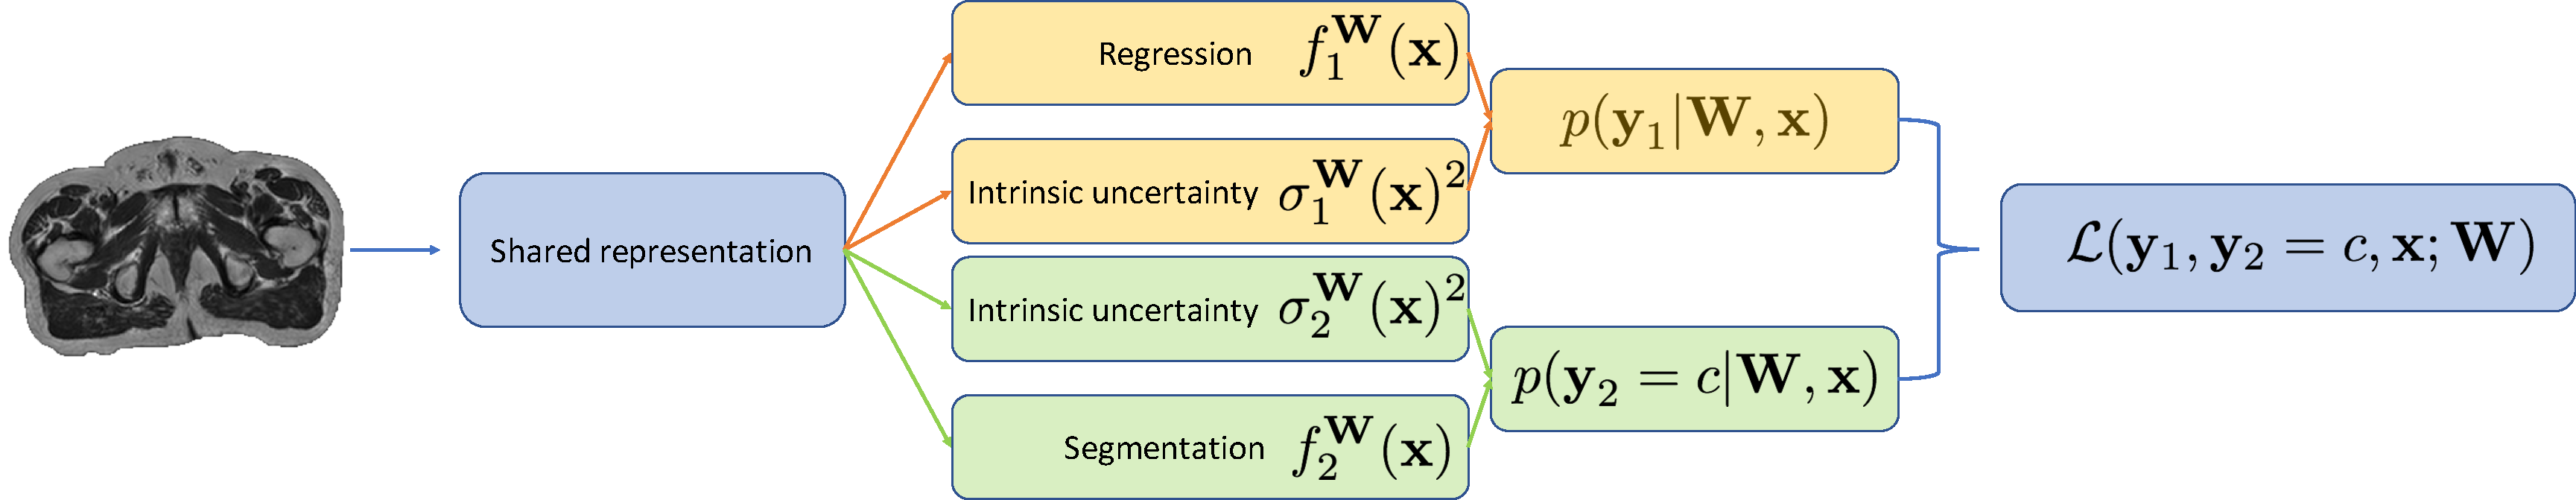
\includegraphics[height=0.185\textwidth]{chapter_5/figures/final_for_ryu_MT.pdf}
		\caption{\footnotesize Multi-task learning architecture. The predictive mean and variance $[f^{\mathbf{W}}_i(\text{\textbf{x}}), \sigma_{i}^{\mathbf{W}}(\text{\textbf{x}})^{2}]$ are estimated for the regression and segmentation. The task-specific likelihoods p$\left(\text{\textbf{y}}_{i}|\text{\textbf{W}},\text{\textbf{x}}\right)$ are combined to yield the multi-task likelihood p$\left(\text{\textbf{y}}_{1}, \text{\textbf{y}}_{2}|\text{\textbf{W}},\mathbf{x}\right)$.} 
		\label{fig:diagram}
	\end{figure}
    
The rationale behind shared layers is to learn a joint representation between two tasks to regularise the learning of features for one task by using cues from the other. We used a high-resolution network architecture (HighResNet) \cite{li2017compactness} as the shared trunk of the model for its compactness and accuracy shown in brain parcellation. HighResNet is a fully convolutional architecture that utilises dilated convolutions and residual connections to produce an end-to-end mapping from an input patch (\textbf{x}) to voxel-wise predictions (\textbf{y}). \diff{The combination of dilated convolution and the residual connections enable the model to integrate efficiently both the short-range (e.g., textures, intensities) and long-range information (e.g., semantic features), both of which are important for the synthesis and anatomical segmentation tasks.}

%The network is capable of representing the data at multiple scales  \todo[color=red!40]{(Ryu): Not sure if this statement is correct. The original dilated conv paper used a context aggregation module which applies 3x3 dilated conv kernels of different dilation factors to the same input features. This allows for multi-scale representation. But, in HighResNet, each dilated conv layer has a fixed dilation factor, right? I agree that this increases the receptive efficiently without pooling.} by increasing the dilation factor of the convolutions at each successive layer. The residual blocks facilitate the modeling of an identity mapping in feature space. Each residual block combines a convolutional layer, an activation layer and a batch-normalisation layer.   

%\subsubsection{Task-specific networks}
% (Ryu) in progress: The final layer of the representation network is split into two task-specific compartments (Fig. \ref{fig:diagram}). Each compartment consists of two networks which operate on the output of representation network and defines the likelihood function $p\left(\text{\textbf{y}}_{i}|f^{\text{\textbf{W}}}(\text{\textbf{x}})\right)$ for each task $i=1, 2$. 

% The goal of each branch is to predict the output of the regression ($y_{1}$), the uncertainty in the regression ($\sigma_{1}$) in addition to the prediction and uncertainty of the segmentation ($y_{2}$ and $\sigma_{2}$). We applied successive convolutional layers with associated activation and batch-normalisation layers to learn task-specific features. Given the predictions, we formulate the likelihood $p\left(\text{\textbf{y}}_{i}|f^{\text{\textbf{W}}}(\text{\textbf{x}})\right)$ for each task $i=1, 2$ given the task-specific estimates and the parameters \textbf{W} for the multi-task network. A joint-likelihood for the network is formulated by considering $p\left(\text{\textbf{y}}_{1},\text{\textbf{y}}_{2}|f^{\text{\textbf{W}}}(\text{\textbf{x}})\right)$ = $\prod_{i} p\left(\text{\textbf{y}}_{i}|f^{\text{\textbf{W}}}(\text{\textbf{x}})\right)$. The methodology for formulating $p\left(\text{\textbf{y}}_{1},\text{\textbf{y}}_{2}|f^{\text{\textbf{W}}}(\text{\textbf{x}})\right)$ with \emph{heteroscedastic} and \emph{parameter} uncertainty is described in the following sections. \todo[color=red!40]{(Ryu) Remove f - just need $p(y|x, W)$. I think the factorisation of lkhd over tasks directly comes from the architecture directly. Will reflect this thought later.}

The final layer of the shared representation is split into two task-specific compartments (Fig. \ref{fig:diagram}). Each compartment consists of two fully convolutional networks which operate on the output of representation network and together learn task-specific representation and define likelihood function $p\left(\text{\textbf{y}}_{i}|\text{\textbf{W}},\textbf{x}\right)$ for each task $i=1, 2$ where \text{\textbf{W}} denotes the set of all parameters of the model. 
%deleted{FELIX] At test time, we use the expectation of these likelihoods as the final estimates for CT intensity value and segmentation label. 
% The final layer of the representation network is split into four individual branches \textcolor{green}{each targeting a specific task: prediction of the regression (resp. segmentation) output $y_{1}$ (resp. $y_{2}$) and of their associated uncertainty $\sigma_1$ (resp. $\sigma_2$)}
% versino 1for each task (Fig. \ref{fig:diagram}). The goal of each branch is to predict the output of the regression ($y_{1}$), the uncertainty in the regression ($\sigma_{1}$) in addition to the prediction and uncertainty of the segmentation ($y_{2}$ and $\sigma_{2}$). Given the predictions, we formulate the likelihood $p\left(\text{\textbf{y}}_{i}|f^{\text{\textbf{W}}}(\text{\textbf{x}})\right)$ for each task $i=1, 2$ given the task-specific estimates and the parameters \textbf{W} for the multi-task network. A joint-likelihood for the network is formulated by considering $p\left(\text{\textbf{y}}_{1},\text{\textbf{y}}_{2}|f^{\text{\textbf{W}}}(\text{\textbf{x}})\right)$ = $\prod_{i} p\left(\text{\textbf{y}}_{i}|f^{\text{\textbf{W}}}(\text{\textbf{x}})\right)$. The methodology for formulating $p\left(\text{\textbf{y}}_{1},\text{\textbf{y}}_{2}|f^{\text{\textbf{W}}}(\text{\textbf{x}})\right)$ with \emph{heteroscedastic} and \emph{parameter} uncertainty is described in the following sections. \todo[color=red!40]{(Ryu) Remove f - just need $p(y|x, W)$. I think the factorisation of lkhd over tasks directly comes from the architecture directly. Will reflect this thought later.}

%A successful probabilistic radiotherapy planning requires both the high quality OAR segmentation, and the Hounsfield Unit prediction along with its associated uncertainty. %\textcolor{green}{some motivation for modelling uncertainty.}
%to better simulate the expected dose delivery . 
\subsection{Task weighting with heteroscedastic uncertainty.}
Previous probabilistic multitask learning methods based on deep learning \cite{kendall2017multi} assumed constant intrinsic uncertainty in respective tasks. In our context, this means that the inherent ambiguity present in synthesis or segmentation tasks do not depend on the spatial locations within an image volume. This is a highly unrealistic assumption since these tasks can be more challenging on some anatomical structures (e.g. tissue boundaries) than others as evidenced by previous work \cite{asman2011robust}. In order to capture potential spatial variation in intrinsic uncertainty, we adapt the \emph{heteroscedastic} (data-dependent) noise model to our multitask learning problem.   

In particular, for the CT synthesis task, we define our likelihood as a normal distribution $p\left(\text{\textbf{y}}_{1}|\mathbf{W},\mathbf{x}\right) = \mathcal{N}(f^{\text{\textbf{W}}}_1(\text{\textbf{x}}), \sigma_{1}^{\text{\textbf{W}}}(\text{\textbf{x}})^{2})$
where mean $f^{\text{\textbf{W}}}_1(\text{\textbf{x}})$ and variance $\sigma_{1}^{\text{\textbf{W}}}(\text{\textbf{x}})^{2}$ are modelled by the regression output and uncertainty branch as functions of the input patch $\mathbf{x}$ (see Fig.\ref{fig:diagram}). We define the task loss for CT synthesis to be the negative log-likelihood $\mathcal{L}_{1}(\text{\textbf{y}}_{1},\mathbf{x};\mathbf{W})= \frac{1}{2\sigma_{1}^{\text{\textbf{W}}}(\text{\textbf{x}})^{2}}||\text{\textbf{y}}_{1}-f^{\text{\textbf{W}}}_1(\text{\textbf{x}})||^{2} + \text{log}\sigma_{1}^{\text{\textbf{W}}}(\text{\textbf{x}})^{2}$. This loss encourages assigning high-uncertainty to regions of high errors, enhancing the robustness of the network against noisy labels and outliers, which are prevalent at organ boundaries especially close to the bone.
%This objective acts as a learned loss attenuation since the network can learn to attenuate the effect of erroneous predictions by predicting higher uncertainty in these regions. This is of particular importance when regressing voxel intensities at organ boundaries especially close the bone, which are prone to errors.
% (version 2) We introduce the \emph{heteroscedastic} noise model to approximate the variation in intrinsic uncertainty across the image. In contrast to \emph{homoscedatic} uncertainty ($\sigma_{i}$) which is assumed constant across the image, \emph{heteroscedasticity} is data-dependent ($\bm{\sigma}_{i}(\text{\textbf{x}})$). For the CT synthesis task, we define our likelihood as a normal distribution with mean given by the regression output $p\left(\text{\textbf{y}}_{1}|\mathbf{W},\mathbf{x}\right) = \mathcal{N}(f^{\text{\textbf{W}}}_1(\text{\textbf{x}}), \sigma_{1}^{\text{\textbf{W}}}(\text{\textbf{x}})^{2})$. The negative log-likelihood is given by $-\text{log}\,p\left(\text{\textbf{y}}_{1}|\mathbf{W},\mathbf{x}\right) = \frac{1}{2\sigma_{1}^{\text{\textbf{W}}}(\text{\textbf{x}})}||\text{\textbf{y}}_{1}-f_{1}(\text{\textbf{x}})^{\text{\textbf{W}}}||^{2} + \text{log}\sigma_{1}^{\text{\textbf{W}}}(\text{\textbf{x}})^{2}$. This likelihood acts as a learned loss attenuation since the network can learn to attenuate the effect of erroneous predictions by predicting higher uncertainty in these regions. This is of particular importance when regressing voxel intensities at organ boundaries especially close the bone, which are prone to errors.

For the segmentation, we define the classification likelihood as softmax function of scaled logits i.e. $p\left(\text{\textbf{y}}_{2}|\textbf{W},\mathbf{x}\right) = \text{Softmax}\big{(}f_{2}^{\text{\textbf{W}}}(\text{\textbf{x}})/\sigma^{\mathbf{W}}_{2}(\text{\textbf{x}})^2\big{)}$ where the segmentation output $f_{2}^{\text{\textbf{W}}}(\text{\textbf{x}})$ is scaled by the uncertainty term $\sigma^{\mathbf{W}}_{2}(\text{\textbf{x}})^2$ before softmax (Fig.\ref{fig:diagram}). As the uncertainty term $\sigma^{\mathbf{W}}_{2}(\text{\textbf{x}})$ increases, the Softmax output approaches a uniform distribution, which corresponds to the maximum entropy discrete distribution. We simplify the scaled Softmax likelihood by considering an approximation used in \cite{kendall2017multi} 
$$\frac{1}{\sigma^{\mathbf{W}}_{2}(\text{\textbf{x}})^2}\sum_{c'}\text{exp}(\frac{1}{\sigma^{\mathbf{W}}_{2}(\text{\textbf{x}})^2}f^{\text{\textbf{W}}}_{2,c'}(\text{\textbf{x}})) \approx \left(\sum_{c'}\text{exp}(f^{\mathbf{W}}_{2,c'}(\text{\textbf{x}}))\right)^{1/\sigma^{\mathbf{W}}_{2}(\text{\textbf{x}})^2}$$ where $c'$ is denotes a segmentation class. This approximation becomes an equality
when $\sigma^{\mathbf{W}}_{2}\rightarrow 1$. This has the advantage of simplifying the
optimisation objective, as well as empirically improving results. This yields the NLL task-loss of the form $\mathcal{L}_{2}(\text{\textbf{y}}_{2}=c,\mathbf{x};\mathbf{W}) \approx \frac{1}{\sigma^{\mathbf{W}}_{2}(\text{\textbf{x}})^2} \text{CE}(f_{2}^{\text{\textbf{W}}}(\text{\textbf{x}}),\text{\textbf{y}}_{2}=c)+ \text{log}\sigma^{\mathbf{W}}_{2}(\text{\textbf{x}})^2$, where CE denotes cross-entropy.
%(f^{\textbf{W}},\textbf{y}}_{2}) + \text{log}\sigma_{2}^{2}(\text{\textbf{x}})
%$\bm{\mathcal{L}}_{2}(\text{\textbf{y}}_{2},\mathbf{x};\mathbf{W}) \approx -\frac{1}{2\sigma^{2}_{2}(\text{\textbf{x}})} \text{log}\left(\text{softmax}(f^{\text{\textbf{W}}}(\text{\textbf{x}}))\right) + \text{log}\sigma_{2}^{2}(\text{\textbf{x}})$. Consequently, the multi-task loss with heteroscedastic weighting that is minimised is:
Finally, assuming that the two tasks $\text{\textbf{y}}_{1},\text{\textbf{y}}_{2}$ are statistically independent given the input image $\mathbf{x}$,  the joint likelihood factorises over tasks  $p\left(\text{\textbf{y}}_{1},\text{\textbf{y}}_{2}|\mathbf{W},\mathbf{x}\right)=p\left(\text{\textbf{y}}_{1}|\mathbf{W},\mathbf{x}\right)p\left(\text{\textbf{y}}_{2}|\mathbf{W},\mathbf{x}\right)$, and thus we can derive the NLL loss for the dual-task model as
\begin{align}
\mathcal{L}(\textbf{y}_{1},\textbf{y}_{2}=c,\mathbf{x};\mathbf{W})
& = - \text{log } p\left(\text{\textbf{y}}_{1},\text{\textbf{y}}_{2}|\mathbf{W},\mathbf{x}\right)\\
&=\frac{||\text{\textbf{y}}_{1}-f^{\text{\textbf{W}}}_1(\text{\textbf{x}})||^{2}}{2\sigma_{1}^{\text{\textbf{W}}}(\text{\textbf{x}})^{2}} + \frac{\text{CE}(f_{2}^{\text{\textbf{W}}}(\text{\textbf{x}}),\text{\textbf{y}}_{2}=c)}{\sigma^{\mathbf{W}}_{2}(\text{\textbf{x}})^2} + \text{log}\Big{(}\sigma^{\mathbf{W}}_{1}(\text{\textbf{x}})^2\sigma^{\mathbf{W}}_{2}(\text{\textbf{x}})^2\Big{)}\;
\end{align}
% \begin{equation}
% \mathcal{L}(\textbf{y}_{1},\textbf{y}_{2}=c,\mathbf{x};\mathbf{W}) = \sum_{i} \frac{1}{\sigma^{\mathbf{W}}_{i}(\text{\textbf{x}})^2}(\textbf{y}_{i},\mathbf{x};\mathbf{W}) + \text{log}\sigma^{\mathbf{W}}_{i}(\text{\textbf{x}})^2 \;
% \end{equation}
where the MSE and CE terms are weighted by the inverse of heteroscedastic intrinsic uncertainty terms $\sigma^{\mathbf{W}}_{i}(\text{\textbf{x}})^2$, that enables automatic weighting of task losses on a per-sample basis. The log-term controls the spread. By contrast, the previous approches resort to spatially constant \cite{kendall2017multi} or manually specified weighting of task losses  \cite{moeskops2016deep,tanno2018autodvt}. 

\subsection{Parameter uncertainty with approximate Bayesian inference.} Analogous to Chapter~\ref{chapter:deepuncertainty}, we approximate the posterior distribution over the network weights using variational inference, and assess the benefit of modelling parameter uncertainty in the context of our multitask learning problem. However, here we instead use the standard binary dropout \cite{srivastava2014dropout} following its Bayesian interpretation introduced by Gal et al.\cite{gal2016dropout}. Let $q(\mathbf{W})$ denote the variational distribution we use to approiximate the true posterior $p(\mathbf{W}|\mathbf{X},\mathbf{Y_1},\mathbf{Y_2})$ where $\mathbf{X} = \{\mathbf{x}^{(1)}, ..., \mathbf{x}^{(N)}\}$, $\mathbf{Y}_1 = \{\mathbf{y}_1^{(1)}, ..., \mathbf{y}_1^{(N)}\}$, $\mathbf{Y}_2	 = \{\mathbf{y}_2^{(1)}, ..., \mathbf{y}_2^{(N)}\}$ is the training data. During training, we minimise the following variational objective similarly to eq.~\eqref{eq:loss_elbo_sr}:  
 \begin{equation}
 \mathcal{L}(\mathcal{D};\mathbf{W}) =  \sum_{(\mathbf{x}^{(i)},\mathbf{y}_1^{(i)},\mathbf{y}_2^{(i)})\in\mathcal{D}} \Big{(}  \mathbb{E}_{q_{\phi}(\text{\textbf{W}})}[- \text{log }p(\mathbf{y}_1^{(i)},\mathbf{y}_2^{(i)}|\mathbf{x}^{(i)},\text{\textbf{W}})]   +  \text{KL} (q(\text{\textbf{W}})||p(\text{\textbf{W}}))\Big{)}
 \end{equation}
 
The second term (referred to as the prior term) is simply given by the L2 weight decay \cite{gal2015dropout}. On the other hand, the first term (referred to as the reconstruction term) cannot be computed exactly, thus we employ the following MC approximation by drawing $S$ samples of network parameters from the approximate posterior $\text{\textbf{W}}^{(s)} \sim q_{\phi}(\text{\textbf{W}})$:
\begin{align*}\label{eq:reconstruction}
\mathbb{E}_{q_{\phi}(\text{\textbf{W}})}[- \text{log }p(\textbf{y}_{1},\textbf{y}_{2}=c|\mathbf{x},\text{\textbf{W}}^{(s)})] 
&\approx \frac{1}{S}\sum_{s=1}^{S} - \text{log }p(\textbf{y}_{1},\textbf{y}_{2}=c|\mathbf{x},\text{\textbf{W}}^{(s)}) \\
&\propto 
\frac{\sum_{s=1}^{S}\sigma_{1}^{\text{\textbf{W}}}(\text{\textbf{x}})^{2}||\text{\textbf{y}}_{1}-f^{\text{\textbf{W}}}_1(\text{\textbf{x}})||^{2}}{2\sum_{s=1}^{S}\sigma_{1}^{\text{\textbf{W}}}(\text{\textbf{x}})^{2}} \\
&+\frac{\sum_{s=1}^{S}\sigma_{2}^{\text{\textbf{W}}}(\text{\textbf{x}})^{2}\text{CE}(f_{2}^{\text{\textbf{W}}^{(s)}}(\text{\textbf{x}}),\text{\textbf{y}}_{2}=c)}{\sum_{s=1}^{S}\sigma^{\mathbf{W}^{(s)}}_{2}(\text{\textbf{x}})^2} \\
&+\sum_{s=1}^{S}\text{log}\Big{(}\sigma^{\mathbf{W}^{(s)}}_{1}(\text{\textbf{x}})^2\sigma^{\mathbf{W}^{(s)}}_{2}(\text{\textbf{x}})^2\Big{)} 
\end{align*}
where the first two terms correspond to the weighted average of the respective task loss functions weighted by the corresponding intrinsic uncertainty. We should also note the slight abuse of notation here; we use $\propto$ to denote the equality up to additive constants. In our experiments we found that the number of samples $S$ per datapoint can be set to 1 as long as the minibatch size was large enough. 

%For each input (or minibatch), we approximate the  reconstruction term using MC approximation by draing network weights from the approximate posterior $w' \sim q(\textbf{\text{W}})$: 
%
%to obtain the multi-task output (predictive mean and predictive variance), $\textbf{f}^{w'}(\text{\textbf{x}}):=[f^{w'}_1(\text{\textbf{x}}),f^{w'}_2(\text{\textbf{x}}), \sigma_{1}^{w'}(\text{\textbf{x}})^{2},\sigma_{2}^{w'}(\text{\textbf{x}})^{2}]$.

%\textcolor{red}{
%We minimize the KL divergence between the approximate posterior $q_{\phi}(\mathcal{W})$ and $p(\mathcal{W}|\textbf{X}, \mathbf{Y}^{(1)}, \mathbf{Y}^{(2)})$. Assuming that the joint likelihood over the two tasks factorizes, we have the following optimization objective:
%\begin{equation}\label{eq:variational_loss}
%\mathcal{L}_{\text{MC}}(\phi) = -\frac{N}{M}\sum_{i=1}^{M} \Big{[}\text{log } p(y^{(1)}_i|\mathbf{x}_i, \mathcal{W}_i) + \text{log }p(y^{(2)}_i|\mathbf{x}_i, \mathcal{W}_i)\Big{]} \\ + \sum_{l=1}^{L}\sum_{k=1}^{K_l}\text{KL}(q_{\phi_{lk}}(\mathbf{W}^{(l),k})||p(\mathbf{W}^{(l),k}))
%\end{equation}
%where $M$ is the size of the mini-batch, $N$ is the total number of training data points, and $\mathcal{W}_i$ denotes a set of model parameters sampled from $q_{\phi}(\mathcal{W})$. The last KL term regularizes the deviation of the approximate posterior from the prior $p(\mathbf{W}^{(l),k})=\mathcal{N}(0, \mathbf{I}/l^{2})$ where $l>0$. Adapting the approximation presented in \cite{gal2016uncertainty} to our scenario, we obtain:
%\begin{equation}\label{eq:KL}
%\text{KL}(q_{\phi_{lk}}(\mathbf{W}^{(l),k})||p(\mathbf{W}^{(l),k})) \propto \frac{l^2}{2}||\mathbf{M}^{(l),k}||^{2}
%_{2} - \mathcal{H}(\mathbf{p}^{(l),k})
%\end{equation}
%where $\mathcal{H}(\mathbf{p}^{(l),k})=-\sum_{i\in \{1,2,s\}}p^{(l),k}_i\text{log }p^{(l),k}_i$ is the entropy of the grouping probabilities. While the first term performs the L2-weight norm, the second term pulls the grouping probabilities towards the uniform distribution. Plugging eq.\eqref{eq:KL} into eq.\eqref{eq:variational_loss} yields the overall loss: 
%\begin{equation}\label{eq:total_loss}
%\mathcal{L}_{\text{MC}}(\phi) = -\frac{N}{M}\sum_{i=1}^{M} \left[\log\text{\,} p\left(y^{(1)}_i|\mathbf{x}_i, \mathcal{W}_i\right) + \log\text{\,} p\left(y^{(2)}_i|\mathbf{x}_i, \mathcal{W}_i\right)\right] \\ + \lambda_{1} \cdot \sum_{l=1}^{L}\sum_{k=1}^{K_l}||\mathbf{M}^{(l),k}||^{2} - \lambda_{2} \cdot \sum_{l=1}^{L}\sum_{k=1}^{K_l}\mathcal{H}(\mathbf{p}^{(l),k})
%\end{equation}
%where $\lambda_1>0, \lambda_2>0$ are regularization coefficients. }



At test time, for each input patch $\textbf{\text{x}}$ in a MR scan, we collect output samples (the mean and variance terms) $\{\textbf{f}^{\,w^{(t)}}(\text{\textbf{x}})\}_{t=1}^{\text{T}}$ where $\textbf{f}^{w'}(\text{\textbf{x}}):=[f^{w'}_1(\text{\textbf{x}}),f^{w'}_2(\text{\textbf{x}}), \sigma_{1}^{w'}(\text{\textbf{x}})^{2},\sigma_{2}^{w'}(\text{\textbf{x}})^{2}]$ by performing $T$ stochastic forward-passes with $\{w^{(t)}\}_{t=1}^{\text{T}}\sim q(\mathbf{W})$. 
To compute the final estimates of synCT and segmentation of OARs, we calculate the mean predictions over the $T$ samples for the respective tasks: 

\begin{equation*}
\hat{\mu}_{\mathbf{y}_j|\mathbf{x}} = \frac{1}{T}\sum_{t=1}^T f^{w^{(t)}}_{j}(\text{\textbf{x}}), \quad j \in \{1,2\}
 \end{equation*}

Finally, we estimate the intrinsic and parameter components of the predictive uncertainty in both tasks by considering the approximations given by eq.~\eqref{eq:sampler_mean} and eq.~\eqref{eq:sampler_var}: 
\begin{align}
\widehat{\Delta}_{m}(\mathbf{y}_j)  &=\frac{1}{T} \sum_{t=1}^{T} f^{w^{(t)}}_{j}(\text{\textbf{x}}) f^{w^{(t)}}_{j}(\text{\textbf{x}})^{\text{T}} -\hat{\mu}_{\mathbf{y}_j|\mathbf{x}} \hat{\mu}_{\mathbf{y}_j|\mathbf{x}}^{\text{T}}\\ 
\widehat{\Delta}_{i}(\mathbf{y}_j)  &= \frac{1}{T} \sum_{t=1}^T \sigma^{w^{(t)}}_{j}(\text{\textbf{x}})^{2}
\end{align}
where $ j \in \{1,2\}$ denotes the task index. As before, the total predictive uncertainty is the sum of the above intrinsic and parameter components. 

%$[\hat{\textbf{\text{y}}}_{1},\hat{\textbf{\text{y}}}_{2},\bm{\hat{\sigma}}^{2}_{1},\bm{\hat{\sigma}}^{2}_{2}]=f^{\bm{\hat{\text{W}}}}(\text{\textbf{x}})$
% At test time, given an input patch in MR scan $\textbf{\text{x}}$, we estimate the predictive distribution $q(\hat{\textbf{\text{y}}}|\hat{\textbf{\text{x}}})$ by sampling from $q(\textbf{\text{W}})$ with $T$ stochastic-samples. For the regression, we calculate the expectation over the $T$ samples in addition to the variance, which is the \emph{parameter} uncertainty. For the segmentation, we perform consider the expectation of class probabilities to obtain the final labels. \emph{Parameter} uncertainty in the segmentation is obtained by considering variance of the stochastic class probabilities. The final predictive uncertainty is the sum of the \emph{intrinsic} and \emph{parameter} uncertainties. This reduces to the the \emph{parameter} uncertainty when no heteroscedastic noise is modelled. 
% During training, network weights are drawn from the approximate posterior $\hat{\text{W}} \sim q(\textbf{\text{W}})$ to obtain the multi-task output with predictive mean and predictive variance $[\hat{\textbf{\text{y}}}_{1},\hat{\textbf{\text{y}}}_{2},\bm{\hat{\sigma}}^{2}_{1},\bm{\hat{\sigma}}^{2}_{2}]=f^{\bm{\hat{\text{W}}}}(\text{\textbf{x}})$. 

% At test time, given an input patch in MR scan $\textbf{\text{x}}$, we estimate the predictive distribution $q(\hat{\textbf{\text{y}}}|\hat{\textbf{\text{x}}})$ by sampling from $q(\textbf{\text{W}})$ with $T$ stochastic-samples. For the regression, we calculate the expectation over the $T$ samples in addition to the variance, which is the \emph{parameter} uncertainty. For the segmentation, we perform consider the expectation of class probabilities to obtain the final labels. \emph{Parameter} uncertainty in the segmentation is obtained by considering variance of the stochastic class probabilities. The final predictive uncertainty in the multi-task network the sum of the \emph{intrinsic} and \emph{parameter} uncertainties. When no heteroscedastic noise is modelled, this uncertainty reduces to the \emph{parameter} uncertainty.



\section{Data Preprocessing and Implementation Details}
\subsection{Data}
We validated on $15$ prostate cancer patients, who each had a T2-weighted MR image (3T, $1.46\times1.46\times5$mm$^{3}$) and a CT image (140kVp, $0.98\times0.98\times1.5$mm$^{3}$) acquired on the day. Organ delineation was performed by a clinician with labels for the left and right femur head, bone, prostate, rectum and bladder. All images were resampled to isotropic resolution. The CT scans were spatially aligned with the T2 scans using the method of Burgos et al. \cite{ninon2017}. In the segmentation, we predicted labels for the background, left/right femur head, prostate, rectum and bladder. The bone region was used for quantifying the synCT.

\subsection{Network architectures and training}\label{sec:imp_details} 
We trained our model on randomly selected 2D axial slices and reconstructed the 3D volume at test time. The representation network was composed of a convolutional layer followed by $3$ sets of twice repeated dilated convolutions \cite{yu2015multi} with dilation factors $[1,2,4]$ and a final convolutional layer. Each layer ($l$) used a $3 \times 3$ kernel with features $f_{R}=[64, 64, 128, 256, 2048]$. Each task-specific branch was a set of $5$ convolutional layers of size $[256_{l=1, 2, 3, 4},n_{i,l=5}]$ where $n_{i,l=5}$ is equal to $1$ for regression and $\bm{\sigma}$ and equal to the number of segmentation classes. The first two layers were $3 \times 3$ kernels whilst the final convolutional layers were fully connected. A Bernouilli drop-out mask with probability $p=0.5$ was applied on the final layer of the representation network. We minimised the loss using the ADAM optimiser \cite{kingma2014adam} with a learning rate $10^{-3}$ and trained for $19,000$ iterations. For the stochastic sampling, we performed model inference $10$ times at iterations $18000$ and $19000$ leading to a set of $T=20$ samples. 

\section{Results}

%\subsubsection{Moved from section 2.3 Implementation details}
%\textcolor{green}{also considered a baseline model to perform single-task regression and segmentation. This was performed with and without drop-out. This baseline was composed of only the representation network with $\nicefrac{1}{2}f_{R}$ and an extra fully-connected layer to output $\text{\textbf{y}}$.}
%\todo[color=green!40]{Integrate the above paragraph into one of the subsections in section 3}


\subsection{Experimental set-up}
We performed a 3-fold cross-validation. Statistics over all hold-out sets are reported. We considered four separate models;  (M1) baseline networks for regression/segmentation, (M2a) baseline network with drop-out for regression/segmentation,  (M2b) the baseline with drop-out and heteroscedastic noise, (M3) multi-task network using homoscedastic task weighting  \cite{kendall2017multi} and (M4) multi-task network using task-specific heteroscedastic noise and drop-out. The baseline networks used only the representation network with $\nicefrac{1}{2}f_{R}$ and a fully-connected layer for the final output. We also compared our results against the current state of the art in atlas propagation (AP) \cite{ninon2017}, which was validated on the same dataset.

\subsection{Model performance}
\begin{table}[!b]
\caption{\footnotesize Model comparison. Bold values indicate where a model was significantly worse than M4 $p<0.05$. No data was available for significance testing with AP. M2b was statistically better $p<0.05$ than M4 in the prostate segmentation.}
\begin{center}
\scalebox{0.90}{
\begin{tabular}{lccccccc}
\toprule
        Models & All & Bone & $L$ femur & $R$ femur & Prostate & Rectum & Bladder \\
\midrule
\multicolumn{8}{c}{Regression - synCT - Mean Absolute Error (HU)} \\
\midrule
M1 			   & \textbf{48.1(4.2)} & \textbf{131(14.0)}  & 78.6(19.2) & \textbf{80.1(19.6)}   & \textbf{37.1(10.4)}  & 63.3(47.3)  & \textbf{24.3(5.2)} \\
M2a 			   & \textbf{47.4(3.0)} & \textbf{130(12.1)}  & 78.0(14.8) & 77.0(13.0)   & \textbf{36.5(7.8)}  & 67(44.6)  & \textbf{24.1(7.5)} \\
M2b \cite{kendall2017uncertainties} & 44.5(3.6) & 128(17.1)  & 75.8(20.1) & 74.2(17.4)   & 31.2(7.0)  & 56.1(45.5)  & 17.8(4.7) \\
M3 \cite{kendall2017multi}& 44.3(3.1) & 126(14.4)  & 74.0(19.5) & 73.7(17.1)   & 29.4(4.7)  & 58.4(48.0) & 18.2(3.5) \\
AP \cite{ninon2017}& 45.7(4.6) & 125(10.3) & - & - & - & - & - \\
M4 (ours) 			   & 43.3(2.9) & 121(12.6)  & 69.7(13.7) & 67.8(13.2)   &28.9(2.9)  & 55.1(48.1) & 18.3(6.1) \\
\midrule
\multicolumn{8}{c}{Segmentation - OAR - Fuzzy DICE score} \\
\midrule
M1 & - & - & 0.91(0.02) & 0.90(0.04) & 0.67(0.12) & 0.70(0.15) & 0.92(0.05) \\
M2a & - & - & 0.85(0.03) & 0.90(0.04) & 0.66(0.12) & 0.69(0.13) & 0.90(0.07) \\
M2b \cite{kendall2017uncertainties} & - & - & 0.92(0.02) & 0.92(0.01) & 0.77(0.07) & 0.74(0.13) & 0.92(0.03) \\
M3 \cite{kendall2017multi}& - & - & 0.92(0.02) & 0.92(0.02) & 0.73(0.07) & 0.76(0.10) & 0.93(0.02) \\
AP \cite{ninon2017} & - & - & 0.89(0.02) & 0.90(0.01) & 0.73(0.06) & 0.77(0.06) & 0.90(0.03) \\
M4 (ours) & - & - & 0.91(0.02) & 0.91(0.02) & 0.70(0.06) & 0.74(0.12) & 0.93(0.04) \\
\bottomrule
\end{tabular}}
\end{center}
\label{tab:table}
\vspace{-10mm}
\end{table}

An example of the model output is shown in Fig.~\ref{fig:diagram2}. We calculated the Mean Absolute Error (MAE) between the predicted and reference scans across the body and at each organ (Tab. \ref{tab:table}). The fuzzy DICE score between the probabilistic segmentation and the reference was calculated for the segmentation (Tab. \ref{tab:table}). Best performance was in our presented method (M4) for the regression across all segmentation masks except at the bladder. Application of the multi-task heteroscedastic network with drop-out (M4) produced the most consistent synCT across all models with the lowest average MAE and the lowest variation across patients ($43.3\pm2.9$ versus $45.7\pm4.6$ \cite{ninon2017} and $44.3\pm3.1$ \cite{kendall2017multi}). This was significantly lower when compared to M1 ($p<0.001$) and M2 ($p<0.001$). This was also observed at the bone and prostate ($p<0.001$). Whilst differences at $p<0.05$ levels of significance was not observed versus M2b and M3, the consistently lower MAE and standard deviation across patients in M4 demonstrates the added benefit of modelling heteroscedastic noise and the inductive transfer from the segmentation task. Moreover, we performed better than the current state of the art in atlas propagation \cite{ninon2017}. Despite equivalence with the state of the art (Tab. \ref{tab:table}), we did not observe any significant differences between our model and the baselines despite an improvement in mean DICE at the smaller organs such as prostate and rectum ($0.70\pm0.06$ and $0.74\pm0.12$) versus the baseline M1 ($0.67\pm0.12$, $0.70\pm0.15$). The \emph{intrinsic uncertainty} (Fig. \ref{fig:diagram2}) captures the uncertainty specific to the data and thus penalises regions of high error, leading to an under-segmentation yet with higher confidence in the result.

%\begin{figure}[!t]
%		\centering
%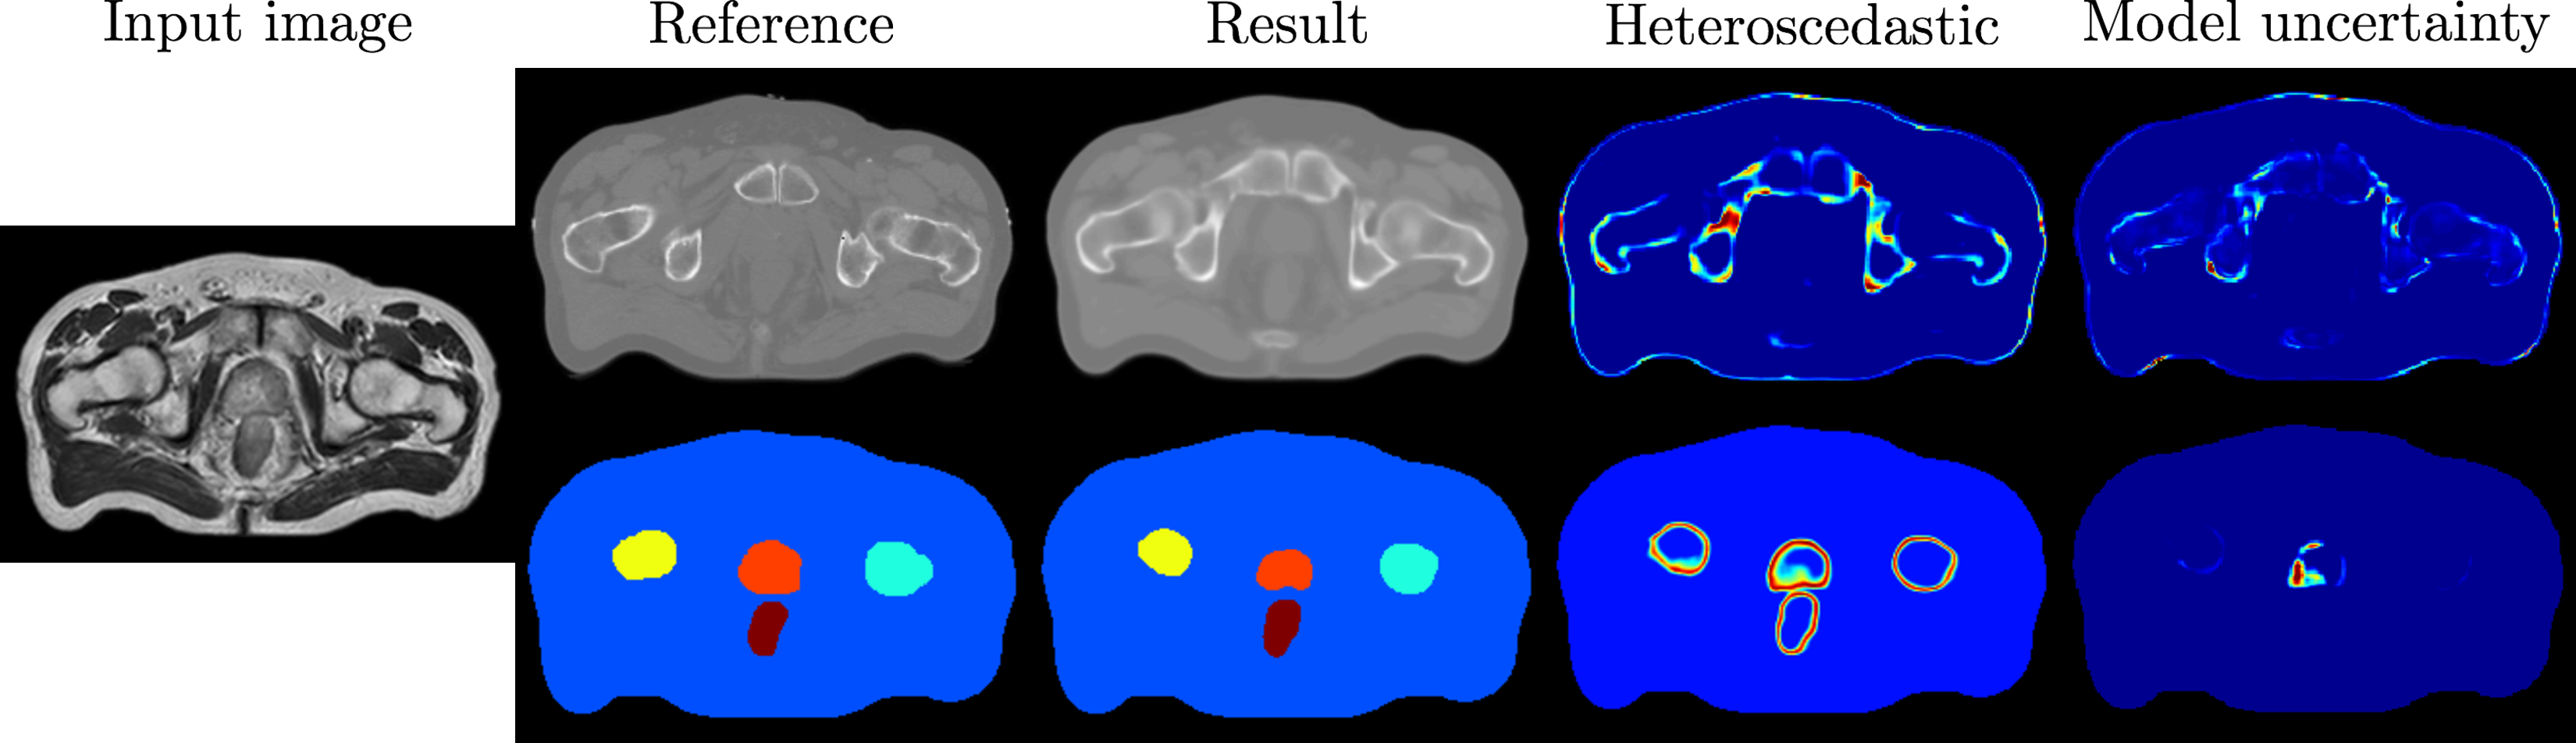
\includegraphics[width=\linewidth]{chapter_5/figures/figure_1_res.pdf}
%		\caption{Example output from the proposed network. The heteroscedastic intrinsic and the parameter uncertainty both correlate strongly with regions of high contrast (bone in the regression), organ boundary (segmentation) and errors in the output.} 
%
%		\label{fig:diagram2}
%        \vspace{-2mm}
%\end{figure}
%


\begin{figure}[!t]
	\centering
	{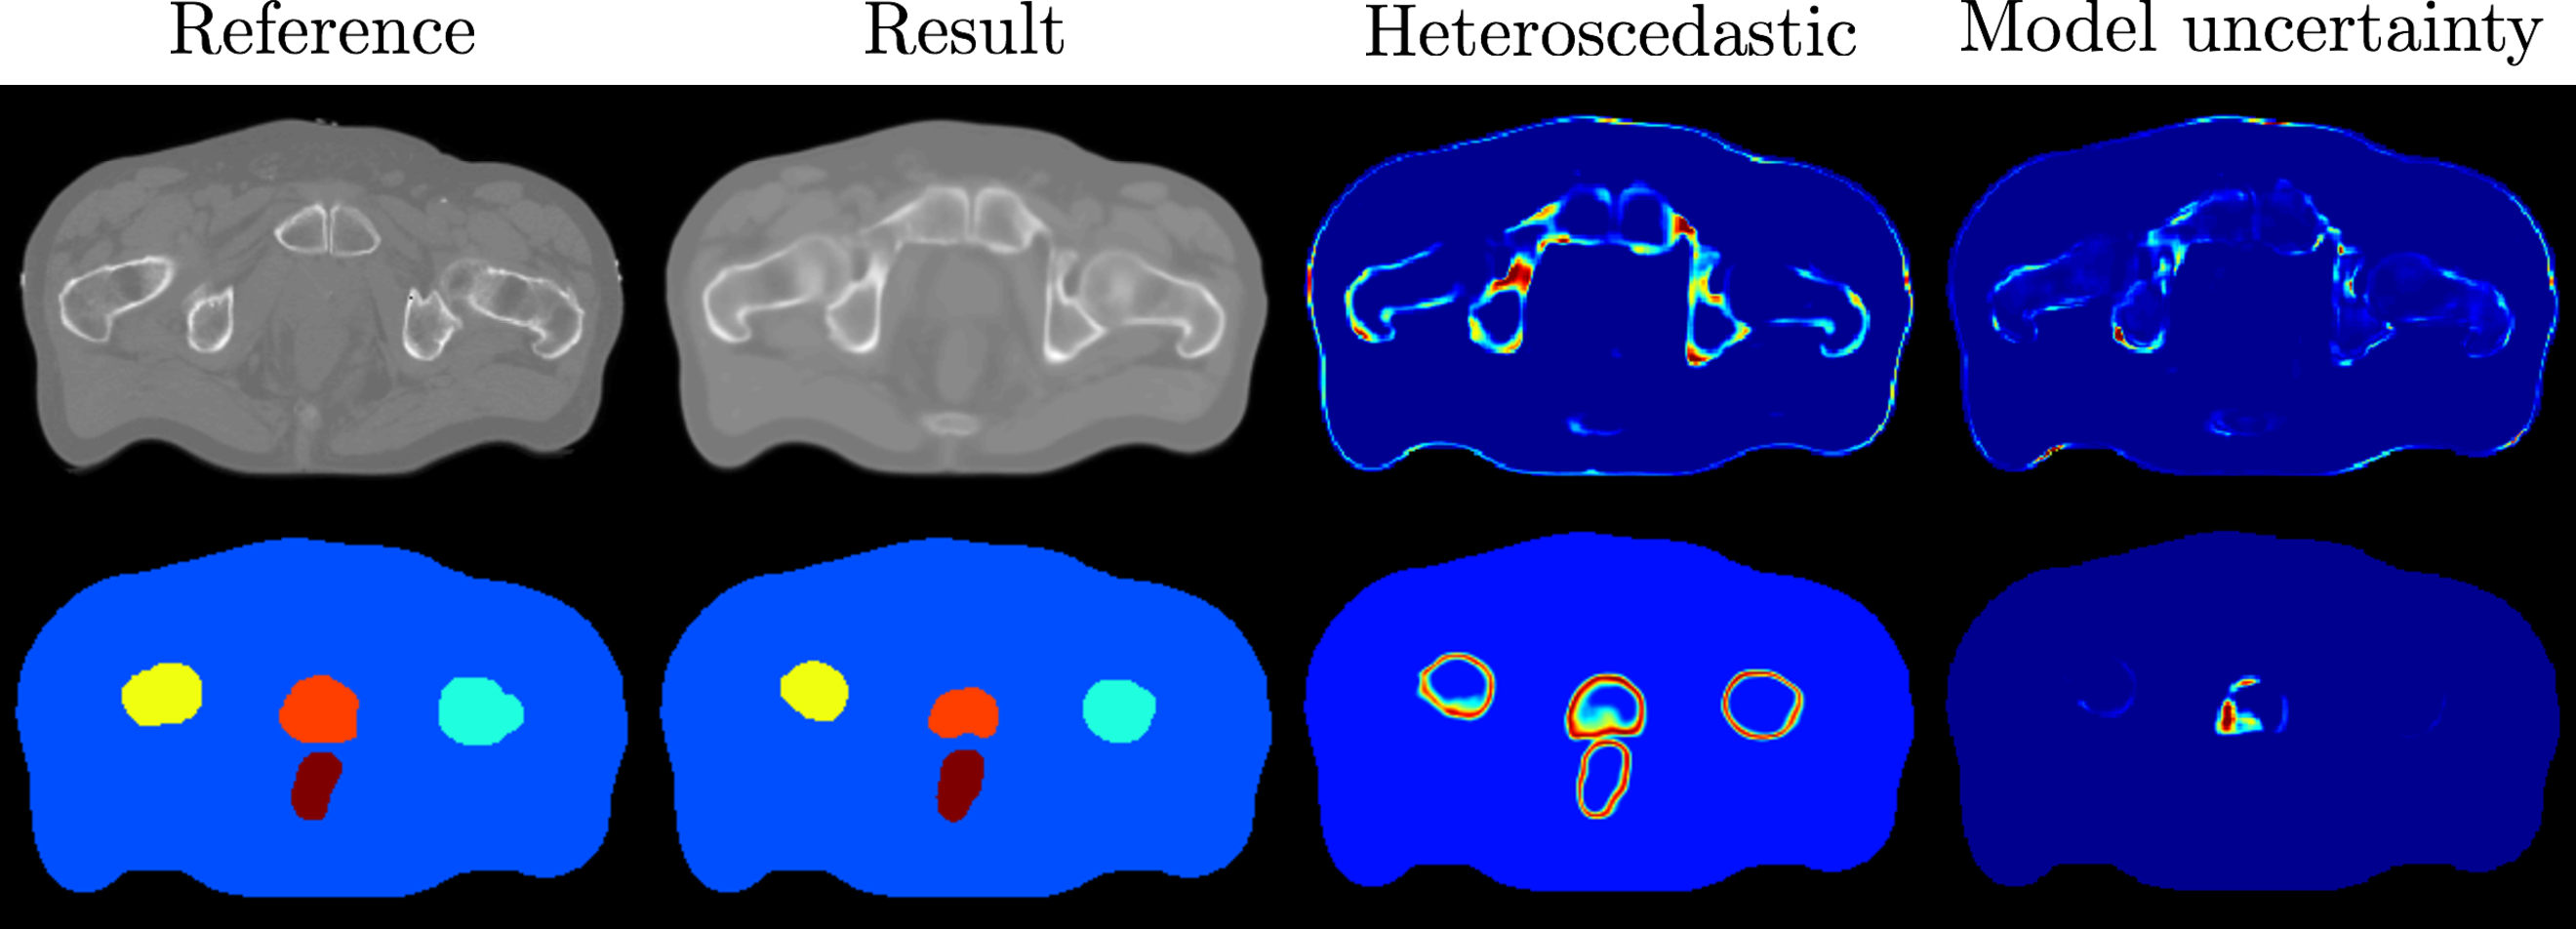
\includegraphics[height=0.21\textwidth]{chapter_5/figures/new_figure_1a.pdf}}%
	\hspace{3pt}
	{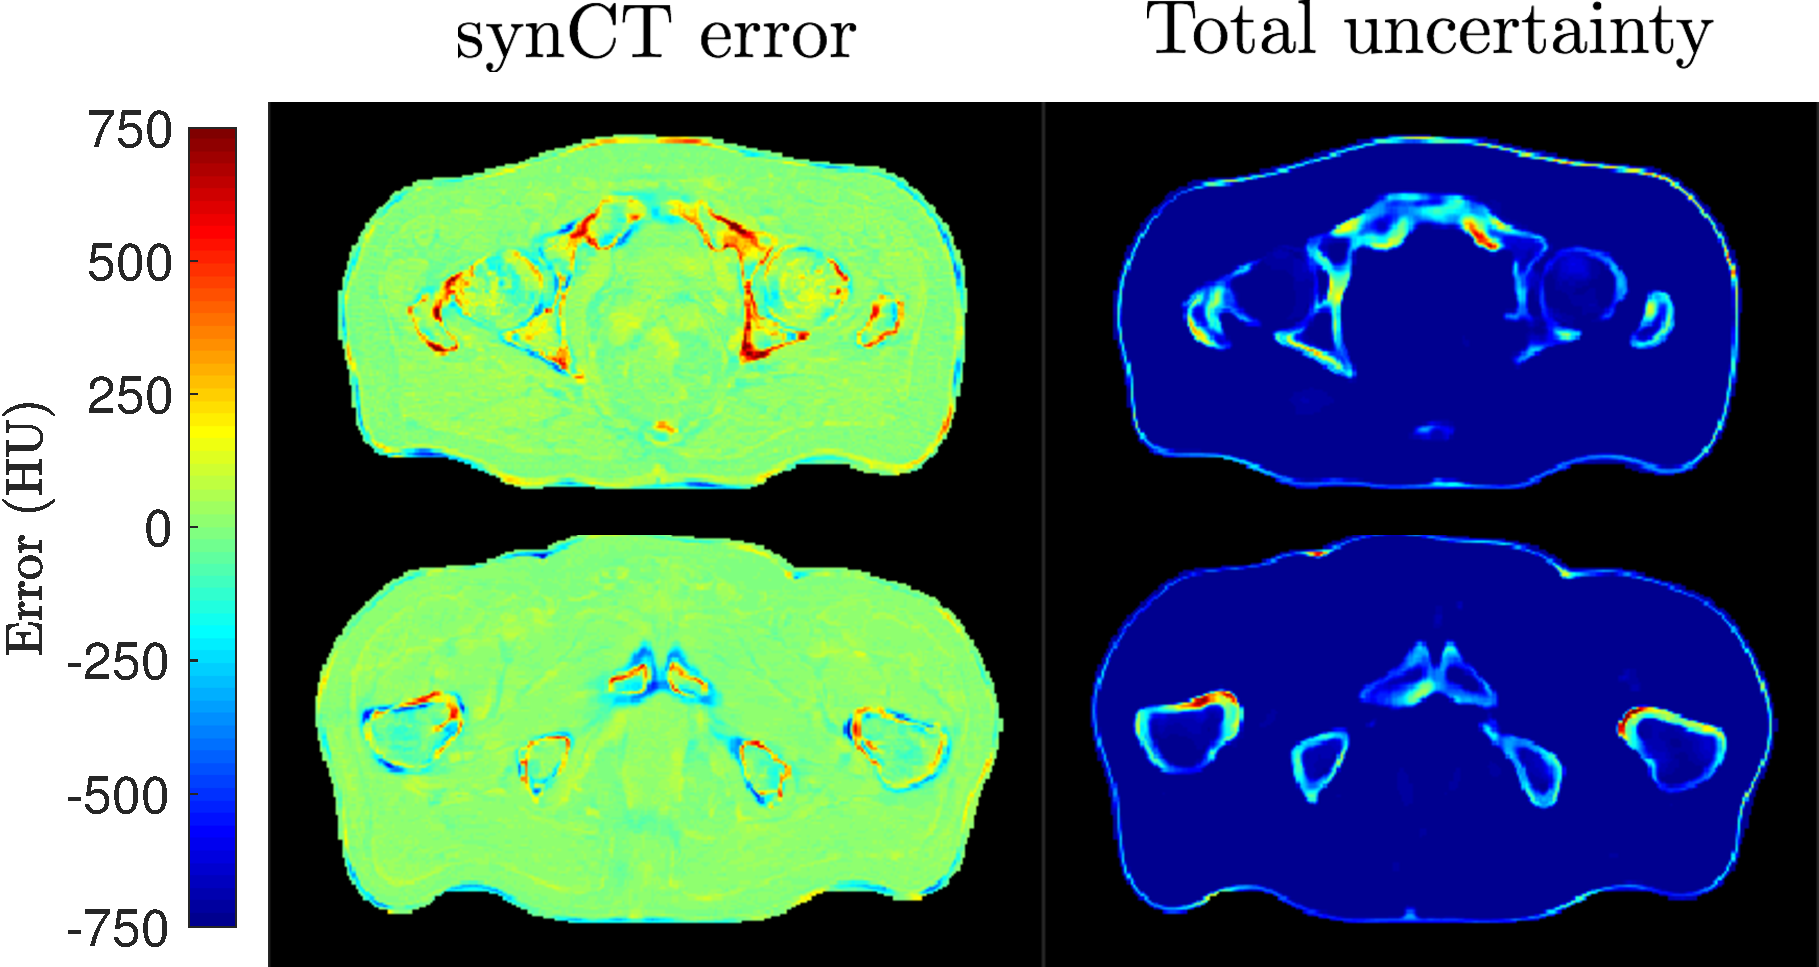
\includegraphics[height=0.21\textwidth]{chapter_5/figures/new_figure_1b.pdf}}%
	\caption{\footnotesize Example outputs from the proposed model. Right: the propagated \textit{intrinsic} (``Heteroscedastic'') and \textit{parameter} (``Model'') uncertainty are shown on an example image for both tasks (CT synthesis and anatomical segmentation) along with the ground truth (``Reference'') and the predictions (``Result''). The uncertainty maps correlate with regions of high contrast (bone in the regression, organ boundary for segmentation). Left: The errors in CT-synthesis (``synCT error'') are compared against the predictive uncertainty (``Total'')---the sum of the heteroscedastic and model uncertainty---on two additional images.  Note the correlation between model error and the predicted uncertainty.}
	\label{fig:diagram2}
\end{figure}


\subsection{Uncertainty estimation for radiotherapy}
We tested the ability of the multi-task heteroscedastic network to better predict associated uncertainties in the synCT error. To verify that our network produces clinically viable samples for treatment planning, we quantified the distribution of regression z-scores for the multi-task heteroscedastic and homoscedastic models. In the former, the total predictive uncertainty is the sum of the propagated \emph{intrinsic} and \emph{parameter} uncertainties, which is used to normalise the error between the synCT and the reference. This should lead to a better approximation of the variance in the model. In contrast, the total uncertainty in the latter reduces to the variance of the stochastic test-time samples. This is likely to lead to a mis-calibrated variance. A $\chi^{2}$ goodness of fit test was performed, showing that the homoscedastic z-score distribution is not normally distributed ($0.82 \pm 0.54$, $p<0.01$) in contrast to the heteroscedastic model ($0.04 \pm 0.84$, $p>0.05$). This is apparent in Fig. \ref{fig:diag3} where there is greater confidence in the synCT produced by our model in contrast the homoscedastic case.

The predictive uncertainty can be exploited for quality assurance (Fig. \ref{fig:diagram4}). There may be issues whereupon time differences have caused variations in bladder and rectum filling across MR and CT scans causing patient variability in the training data. This is exemplified by large errors in the synCT at the rectum (Fig. \ref{fig:diagram4}) and quantified by large localised z-scores (Fig. \ref{fig:diagram4}g), which correlate strongly with the propagated \emph{intrinsic} and \emph{parameter} uncertainty across tasks.

\begin{figure}[!t]
	\centering
	{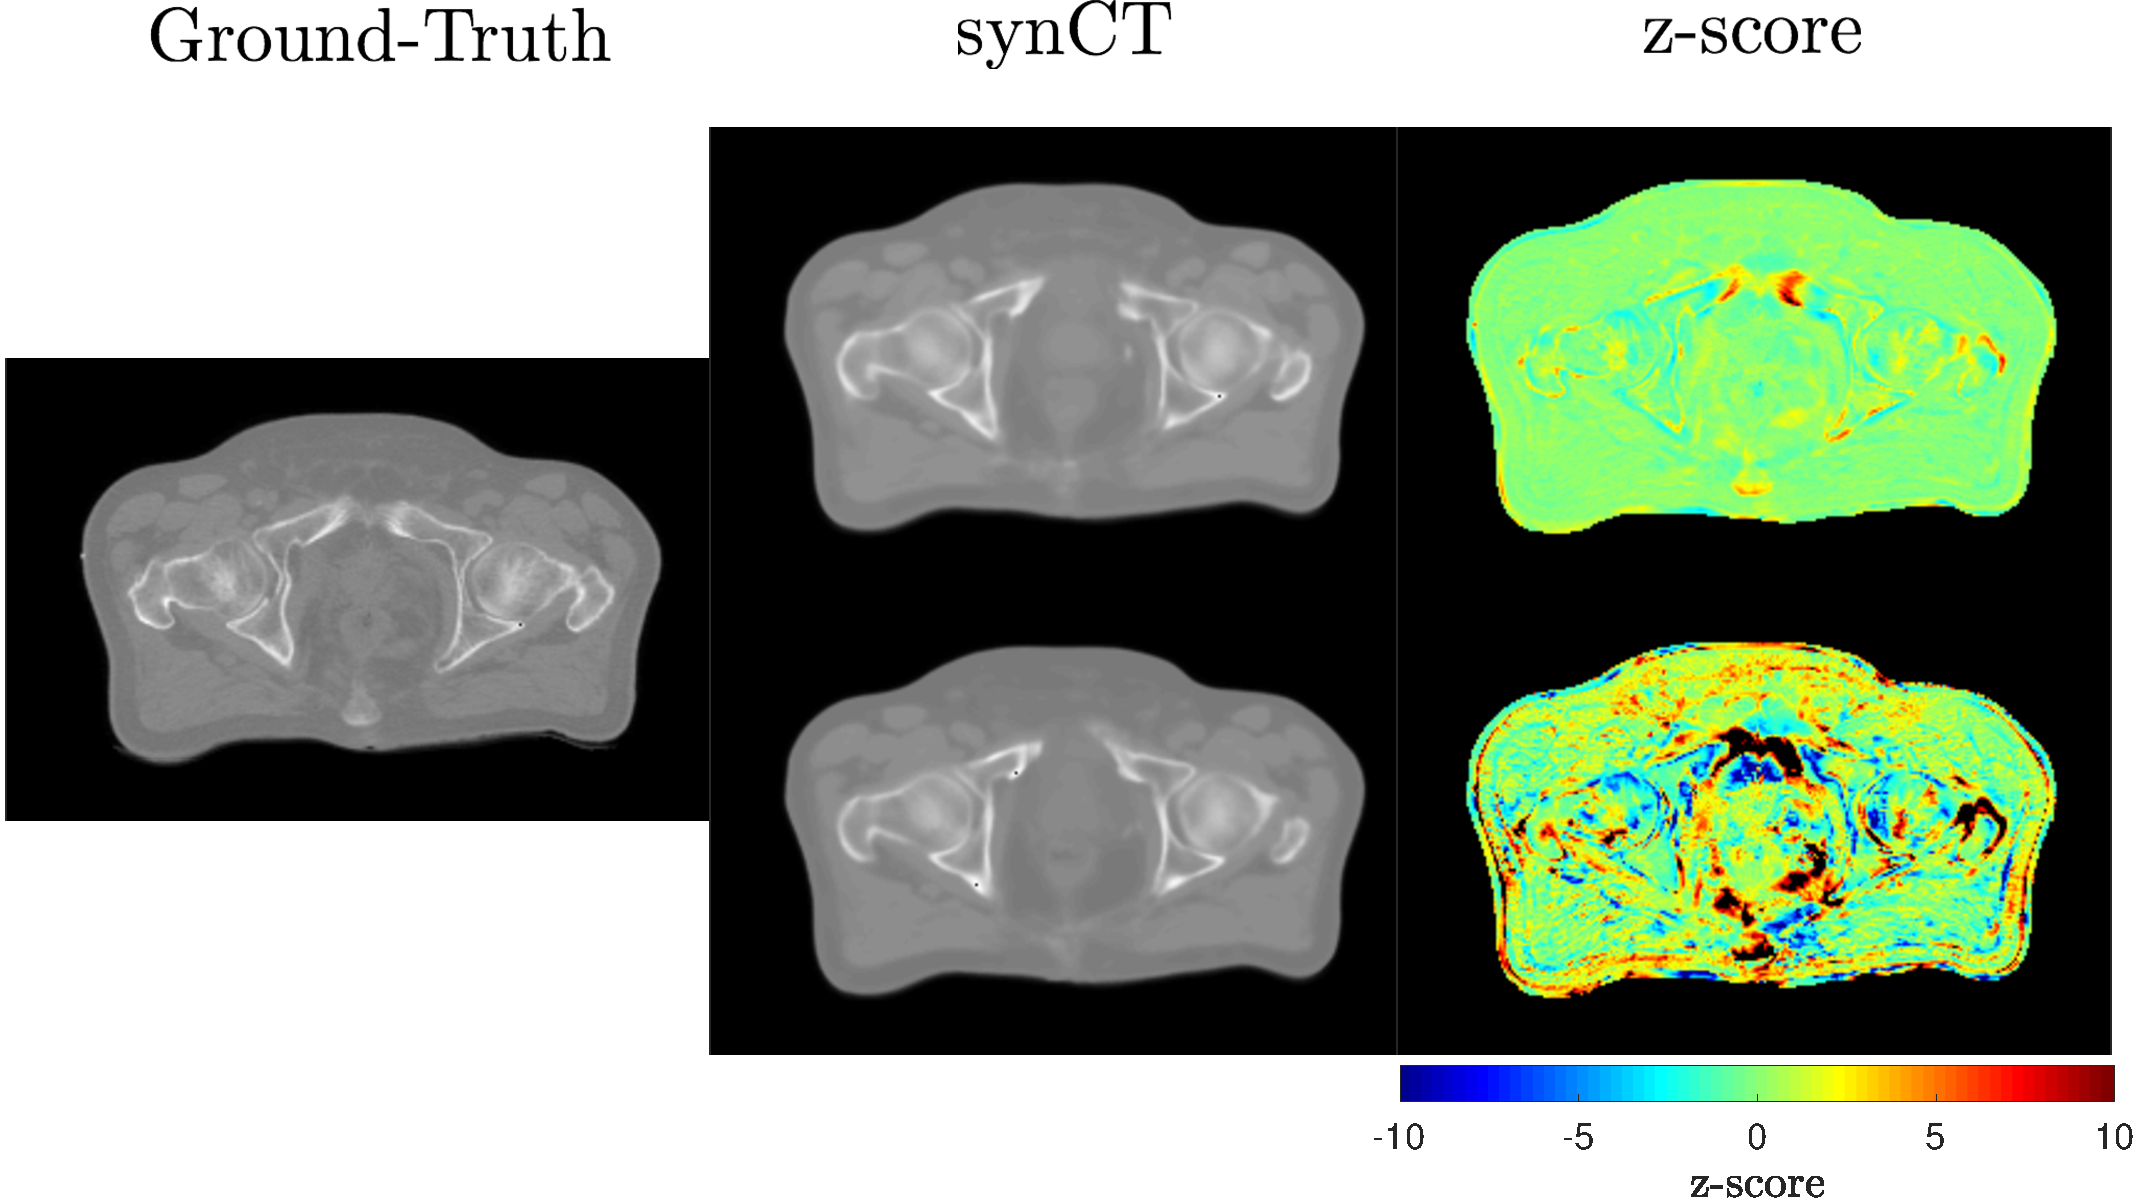
\includegraphics[trim=0mm 0mm 0mm 0mm,clip=true,height=0.29\textwidth,keepaspectratio]{chapter_5/figures/new_fig_z_1.pdf}}
	\hspace{0.01\textwidth}
	{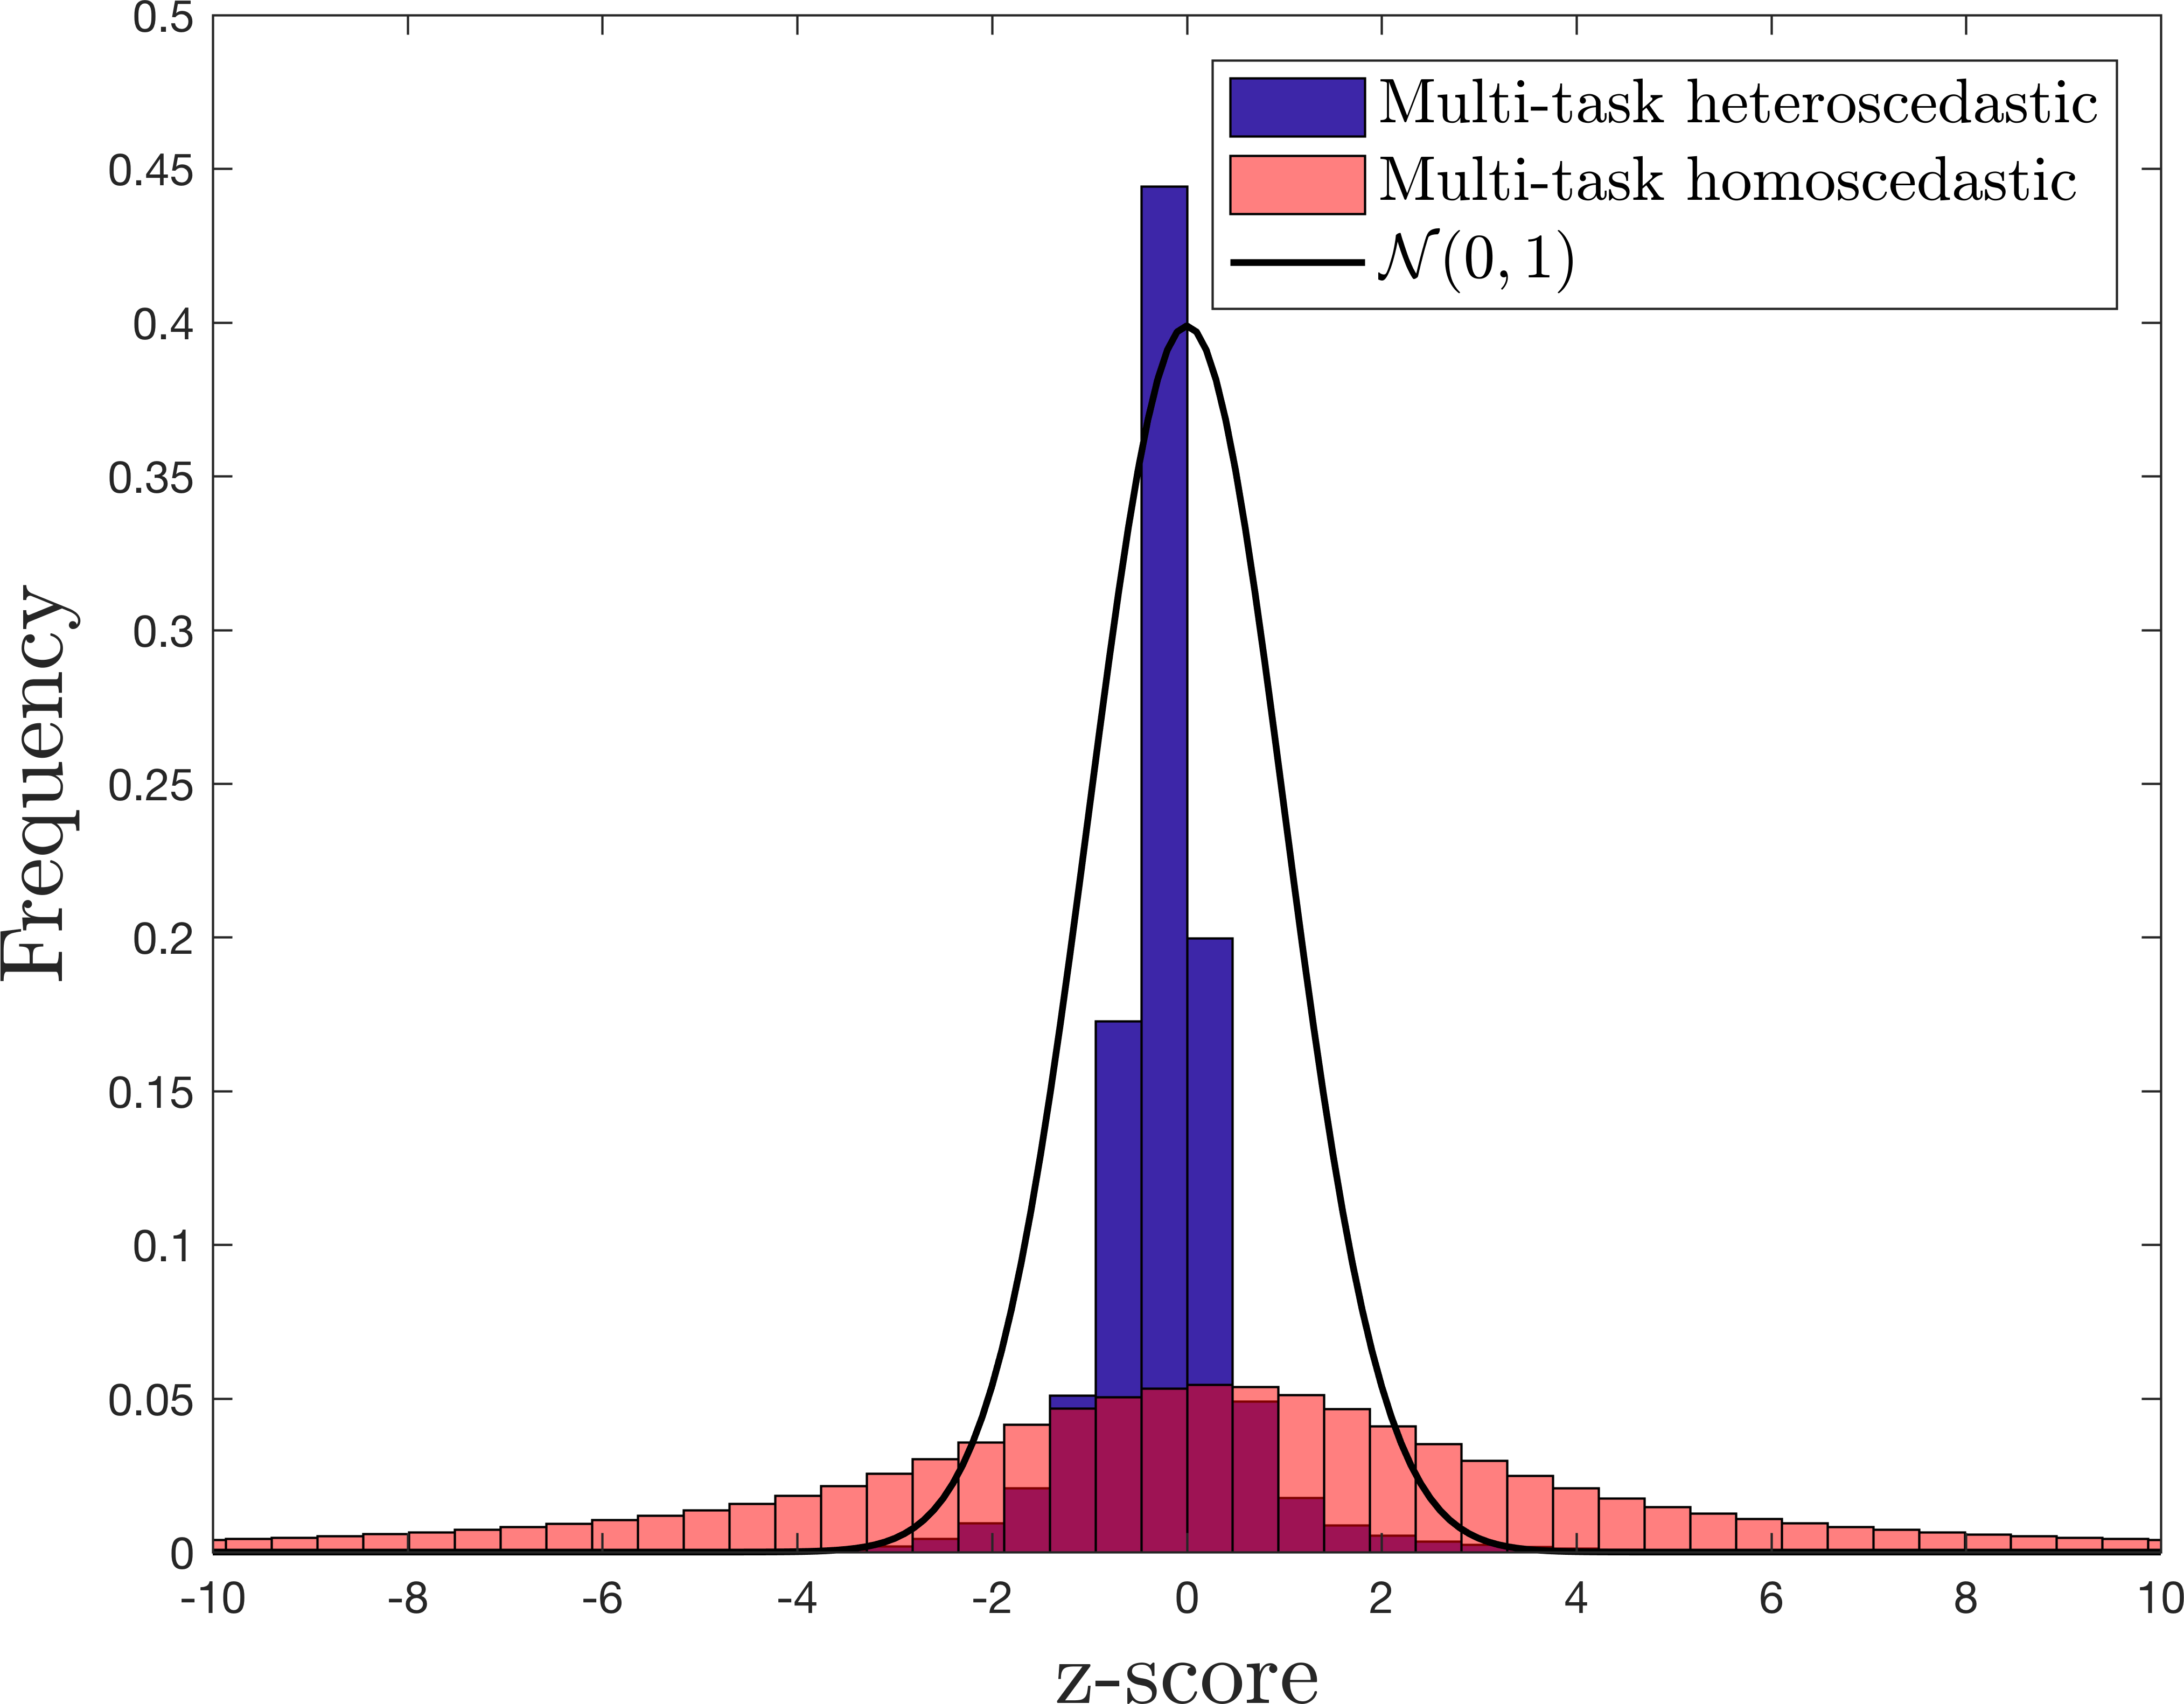
\includegraphics[trim=0mm 0mm 0mm 0mm,clip=true,height=0.29\textwidth,keepaspectratio]{chapter_5/figures/fig_z_2.png}}
	\caption{\footnotesize Analysis of uncertainty estimation. a) synCTs and z-scores for the a subject between M4 (top) and M3 (bottom) models. b) z-score distribution of all patients ($15$) between both models.}
	\label{fig:diag3}
\end{figure}

%\begin{figure}[!t]
%  \centering
%	\begin{subfigure}[]{0.75\linewidth}
%		\caption{Comparison of error quantification}	
%		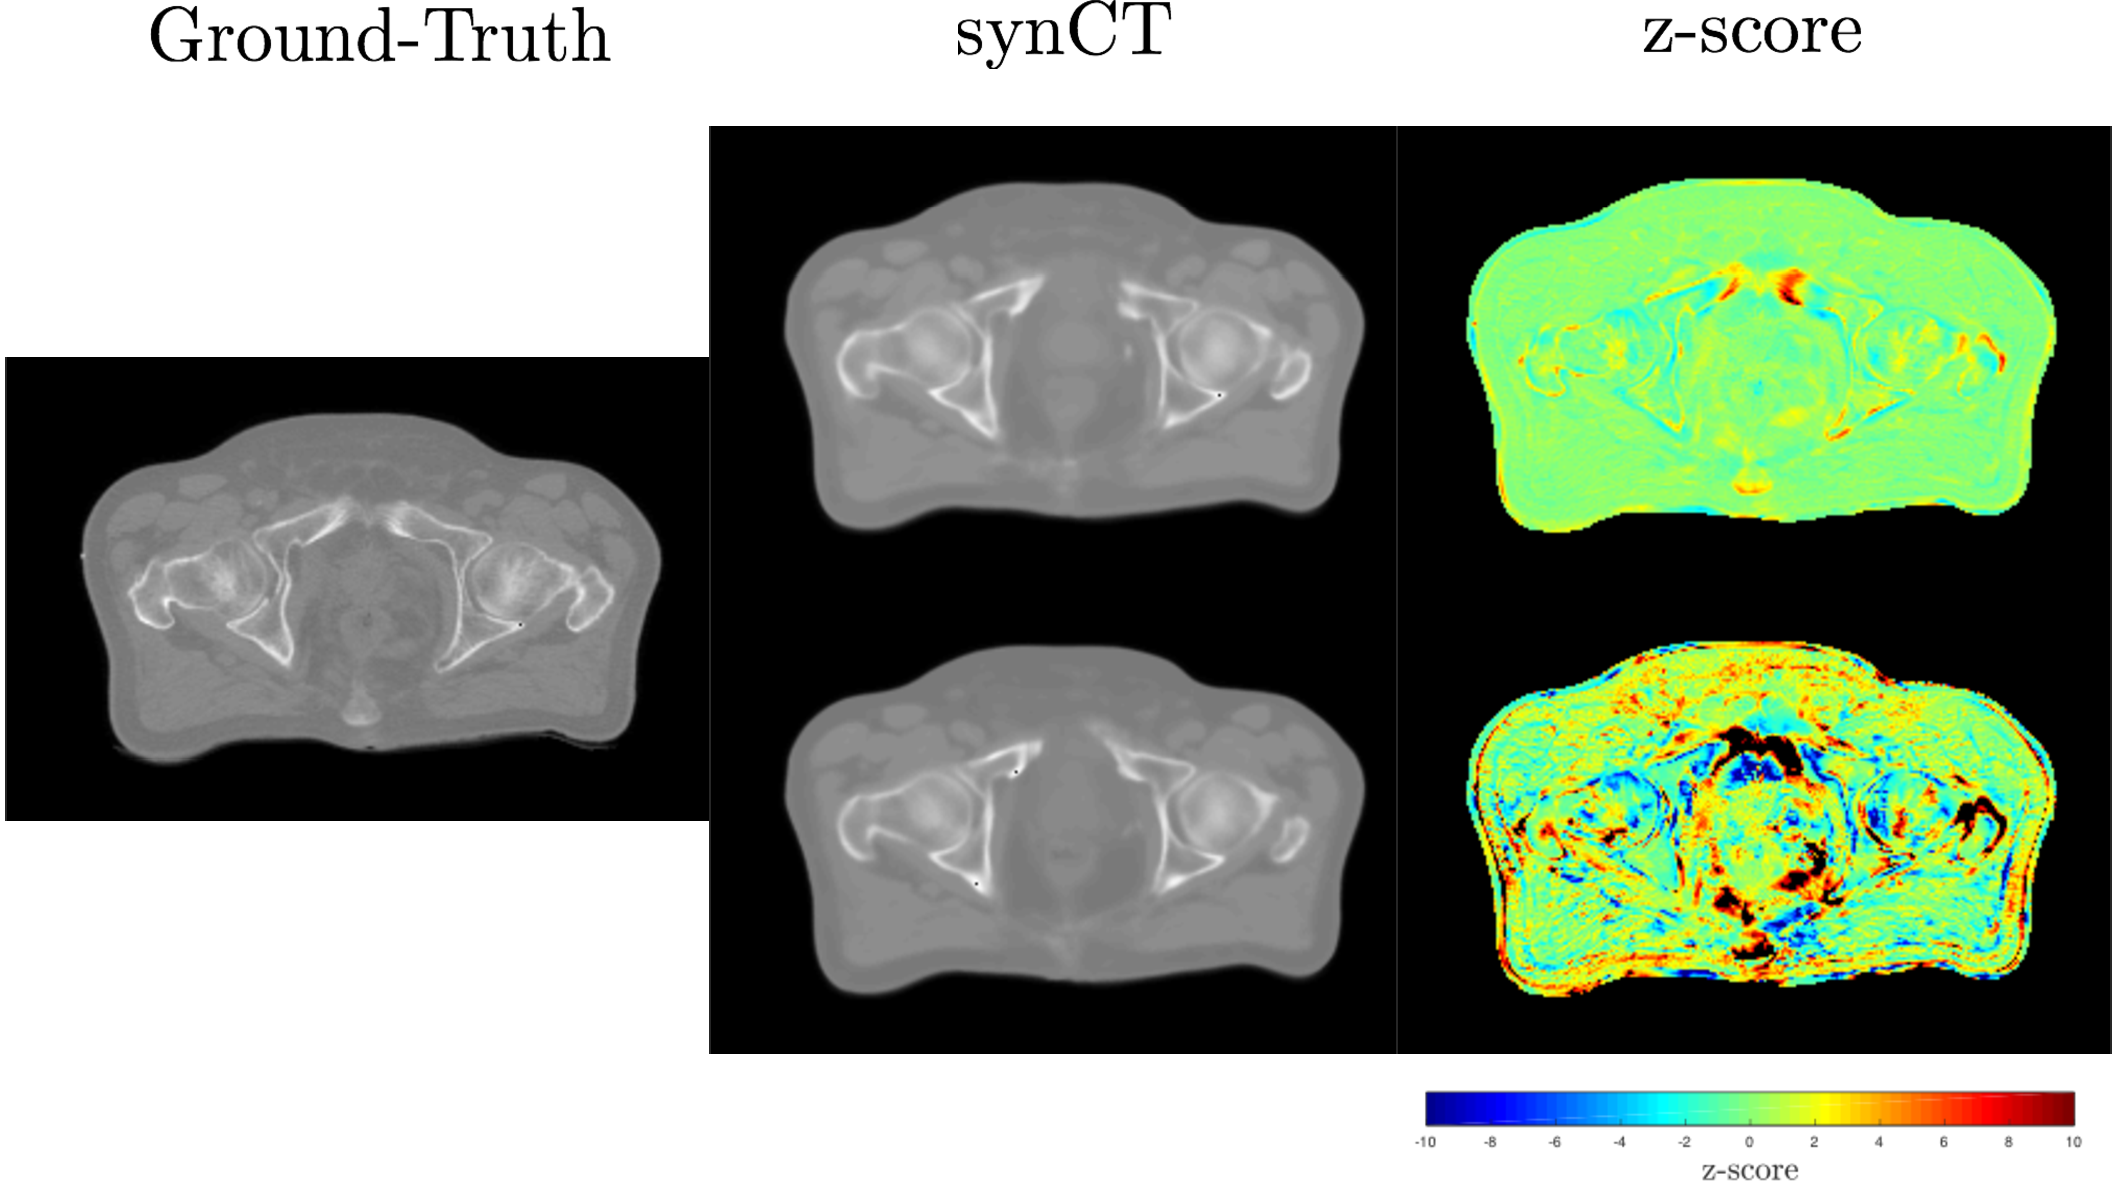
\includegraphics[width=\linewidth]{chapter_5/figures/fig_z_1.pdf}
%	\end{subfigure}
%	\begin{subfigure}[]{0.7\linewidth}
%		\caption{z-score distribution}
%		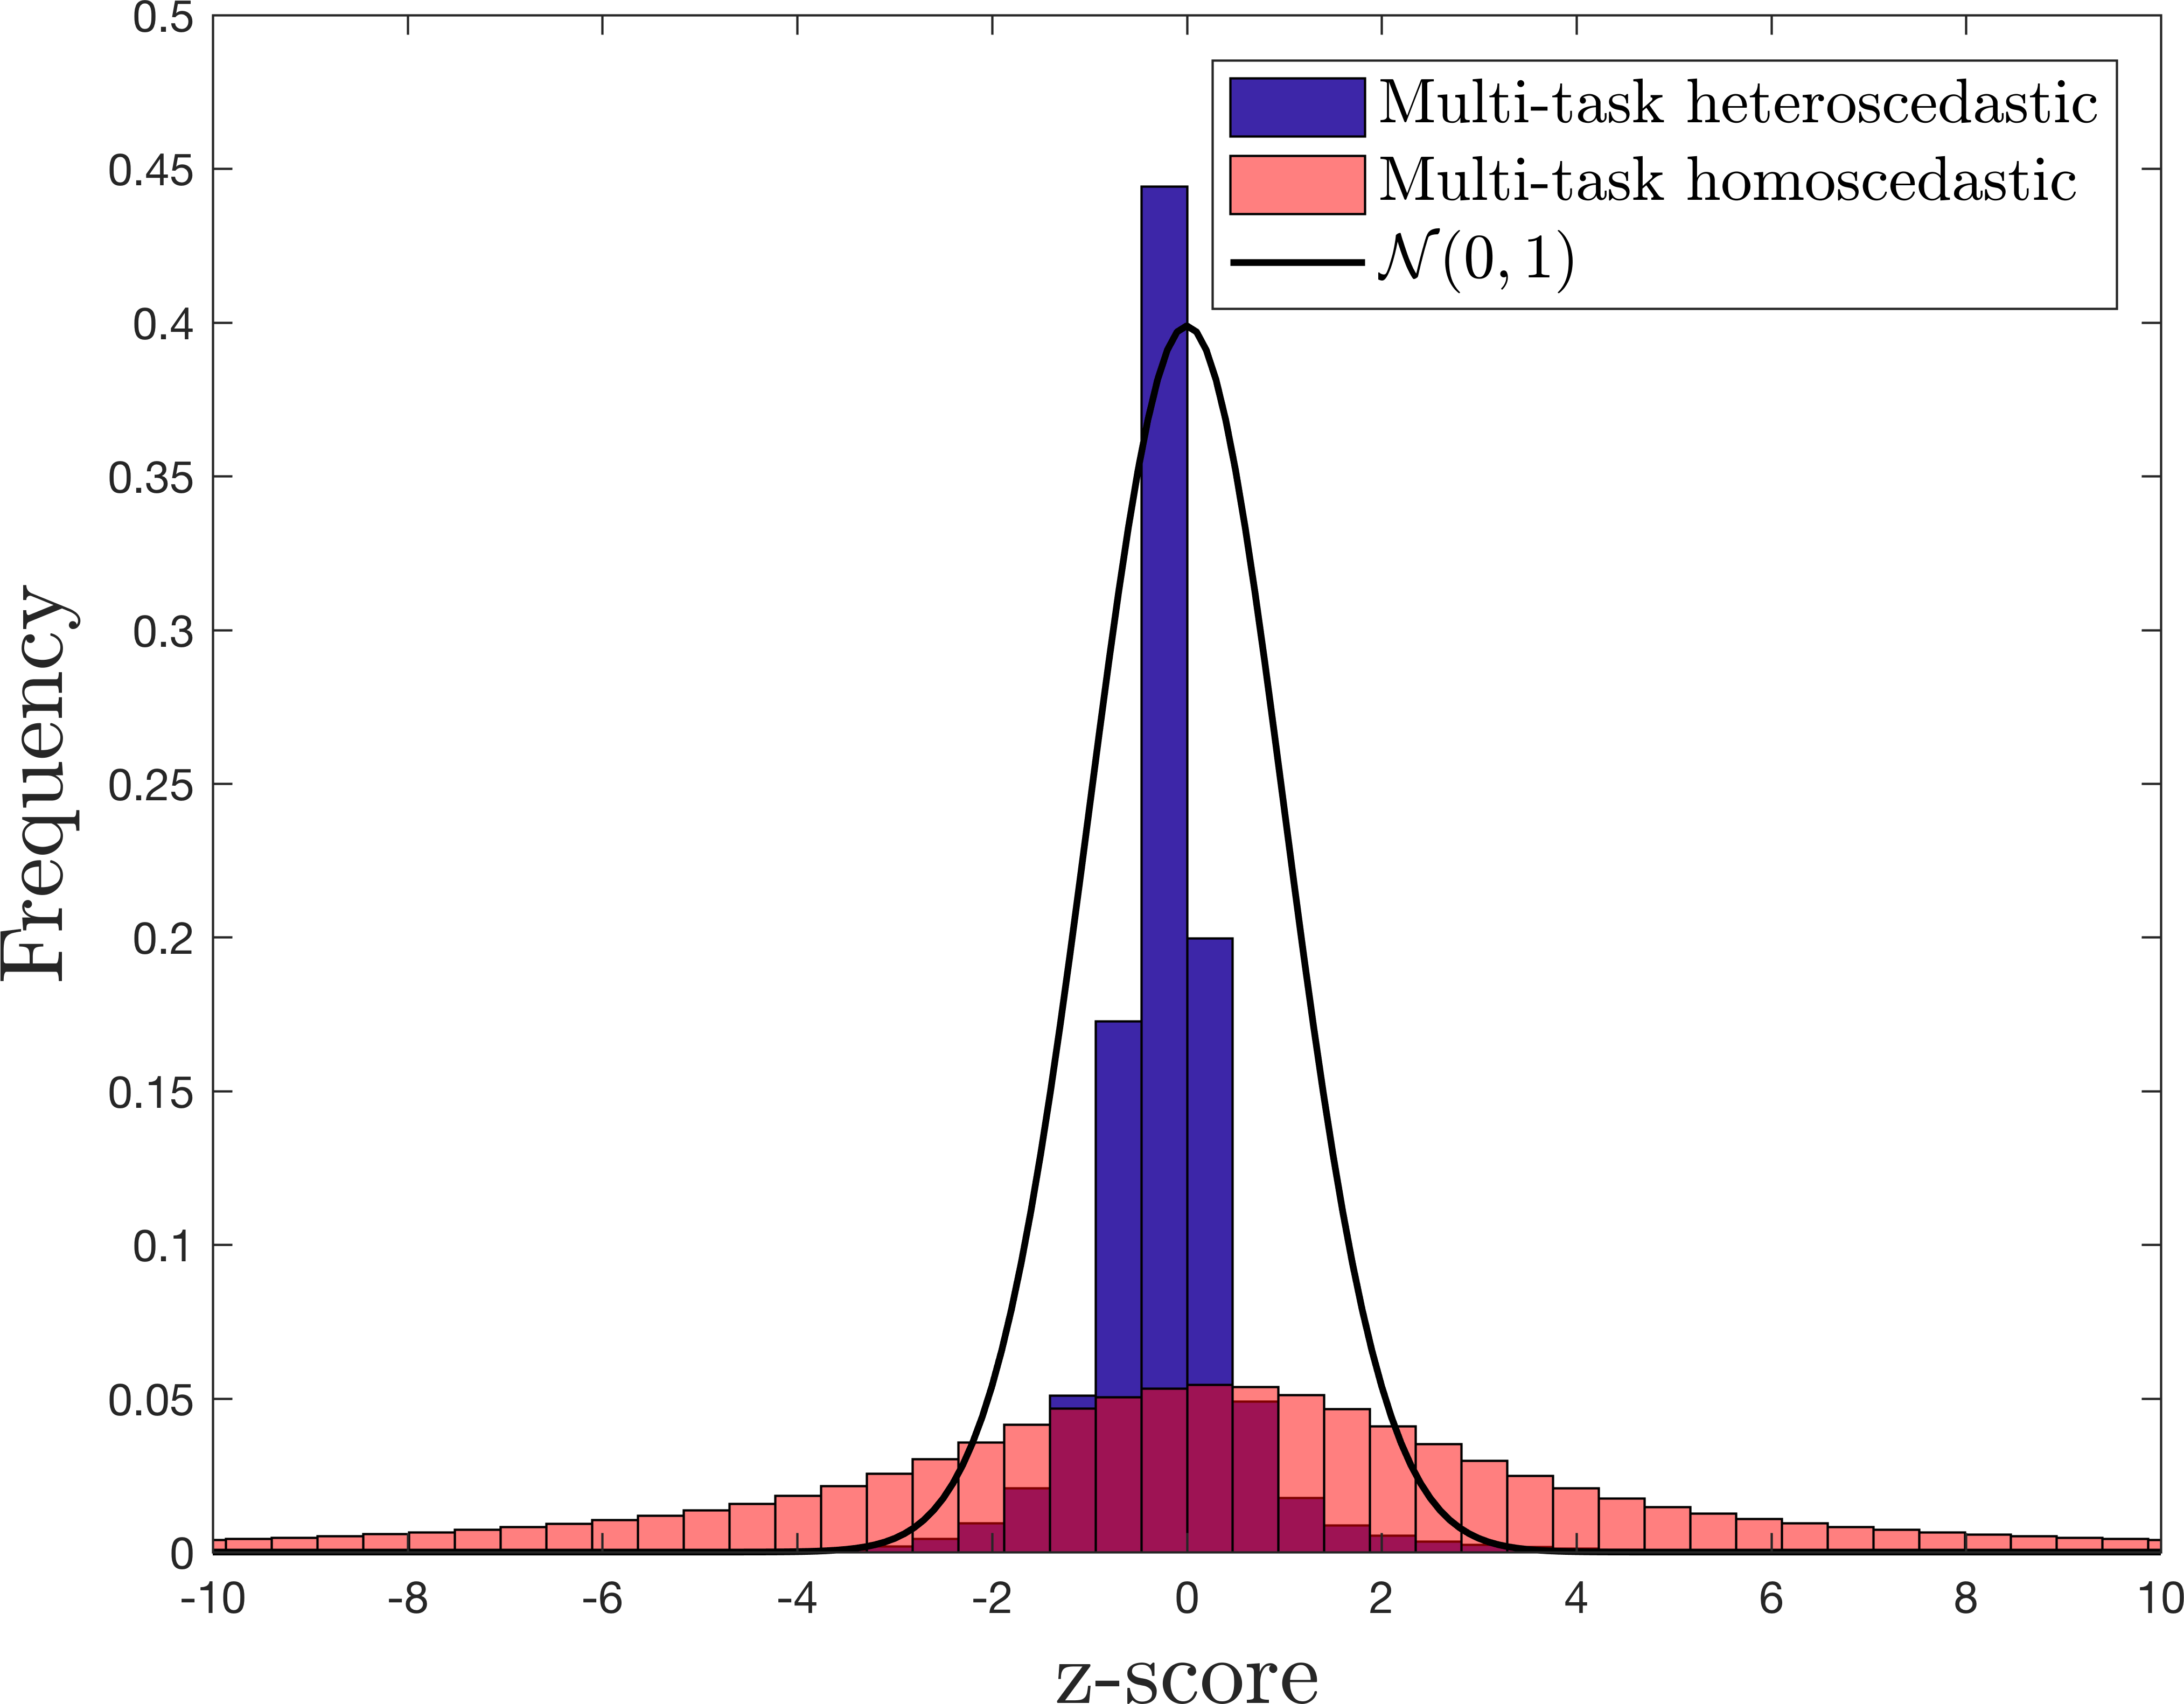
\includegraphics[width=\linewidth]{chapter_5/figures/fig_z_2.png}
%	\end{subfigure}
%	\caption{a) synCTs and z-scores for the same subject between M4 (top) and M3 (bottom) models. b) z-score distribution of all patients ($15$) between both models.}
%	\label{fig:diag3}
%\end{figure}

\begin{figure}[!t]
	\centering
	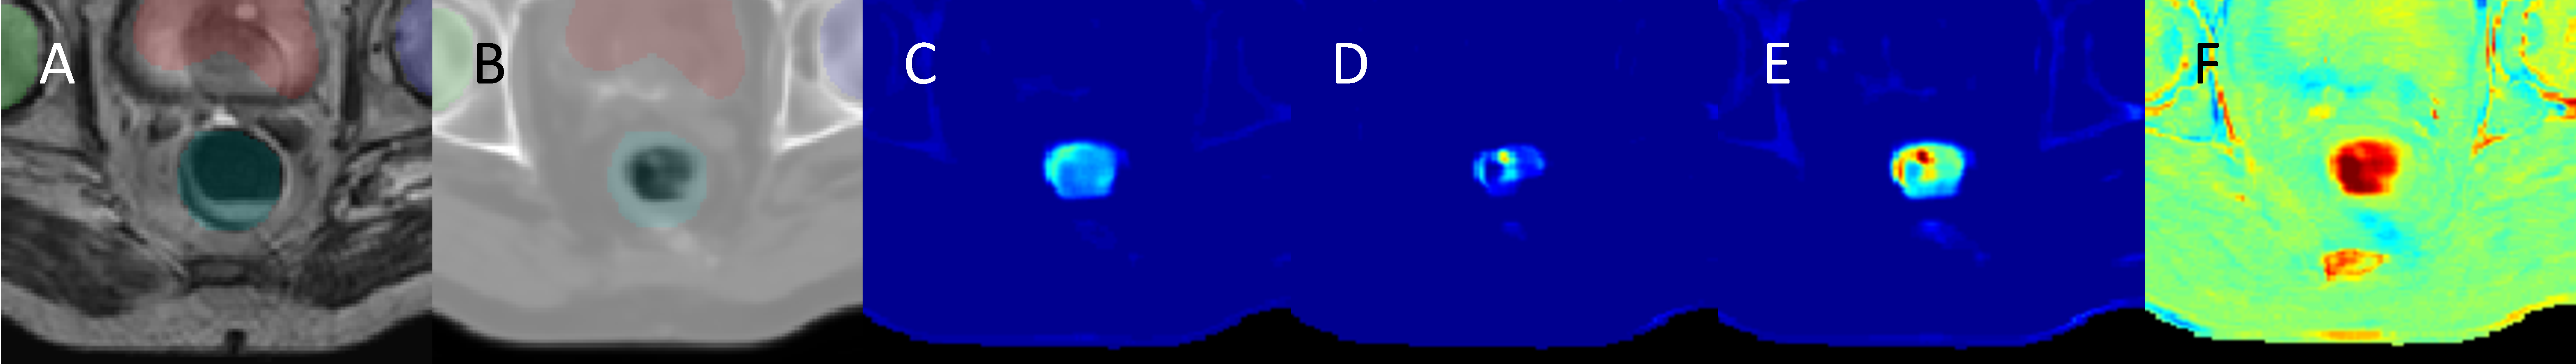
\includegraphics[width=\linewidth]{chapter_5/figures/new_qa.pdf}
	\caption{\footnotesize Uncertainty in problematic areas. a) T2 with reference segmentation, b) synCT with localised errors at the rectum, c) propagated intrinsic uncertainty in synCT, d) propagated parameter uncertainty in synCT, e) total predictive uncertainty and f) error in HU (range [-750HU, 750HU]).} 
	\label{fig:diagram4}
\end{figure}

\section{Conclusions}
%
%\textcolor{red}{Applications of uncertainty information for quality assurance: mention that the future work will study the downstream utility of the uncertainty information to design a safer treatment planning of radiotherapy. For example, you could cite \cite{sands2015utilisation,tilly2019probabilistic}.}
%
%\textcolor{red}{Also mention that as already discussed in the discussion section of Chapter~\ref{chapter:deepuncertainty}, the limitations of the introduced uncertainty modelling techniques, such as, the unimodality of the likelihood and the inflexibility of the posterior distributions, are equally applicable here. }
We have adapted the methods of uncertainty modelling introduced in Chapter~\ref{chapter:deepuncertainty} to the multi-task learning setting. Our network extends prior work in multi-task learning by integrating heteroscedastic uncertainty modelling to naturally weight task losses and thus facilitate inductive transfer between tasks. We have demonstrated the applicability of our network in the context of MR-only radiotherapy treatment planning where the synthetic CT scan (SynCT) and the segmentation of OARs are simultaneuously generated from the input MR image. We have shown that accounting for uncertainty information leads to more accurate and consistent synCTs with a constraint on anatomical consistency with the segmentations. Importantly, we have demonstrated that the output of our network leads to consistent anatomically correct stochastic synCT samples that can potentially be effective in treatment planning. Furthermore, we have also shown that the estimates of predictive uncertainty with our method is more calibrated than the equivalent model with homoscedastic noise model. In the future work, we will evaluate the downstream utility of such uncertainty information in the predicted synCT and OAR segmentation in designing a safer treatment planning of radiotherapy e.g., \cite{sands2015utilisation,tilly2019probabilistic}.
 



%delted: as they assume that the given solution is correct
% (version 1):
% Classical methods for simulating a synCT and segmenting corresponding MR scans have originated from multi-atlas propagation [refNinon]. However, they are severely limited in view of current dose delivery systems. cThis is interesting. So doctors already work with uncertainty? How is this obtained?} Dose delivery in tissue is commonly estimated in a probabilistic setting through Monte Carlo (MC) simulation. Current methods [refNinon, someoneElse] are deterministic and cannot provide estimates of uncertainty in the synCT. However, by sampling the predictive distribution of the model that generates the synCT, a sample can be provided at every MC iteration [ref?] to increase the accuracy of the dose delivery plan \todo[color=red!40]{In the last sentence, may be we can simply contrast with the previous sentence and say: Probabilistic approaches, on the other hand, provide a distribution over the predicted synCT, enhancing the quality of the dose delivery plan.}. 

% (version 2) 
% More recently, applications of convolutional neural networks (CNNs) to CT synthesis from MRI has become a topic of growing interest due to their reconstruction performance, covering range of anatomy from the brain [Han2017] to the pelvic area [Nie2017, DLMIA]. To alleviate the problem of lacking high-frequency information in synCT due to mean-squared reconstruction loss, [Nie2017, arxiv] employed a conditional generative adversarial network \cite{goodfellow2014generative} to capture fine texture details. Wolterink et al. [Wolterink2017, SASHIMI2017] extended this idea using a CycleGAN \cite{zhu2017unpaired} to leverage more abundant misaligned or possibly unpaired training sets of CR and MR scans. Despite this progress, the same problem in common with the classical methods remains; these algorithms typically commit to a single prediction, with no measure of uncertainty. Moreover, they also do not attempt to segment the OARS, which is necessary in radiotherapy planning.
% (version 1) More recently, applications of convolutional neural networks (CNNs) to CT synthesis from MRI has become a topic of growing interest due to their reconstruction performance, covering range of anatomy from the brain [Han2017] to the pelvic area [Nie2017, DLMIA]. However, these solutions required a training set with spatially aligned MR and CT scans, whereupon misalignments in data preprocessing may induce errors in the synCTs. To alleviate this issue, networks employing an adverserial training strategy have recently been developed [Nie2017, Wolterink2017]. Nie et al. [Nie2017, arxiv] combined a voxel-wise loss with an image-wide adversarial loss in a generative adversarial network \cite{goodfellow2014generative} whilst Wolterink et al. [Wolterink2017, SASHIMI2017] extended this idea using a CycleGAN \cite{zhu2017unpaired}. Despite this progress, these methods typically commit to a single prediction, with no measure of predictive uncertainty that could be exploited by modern planning systems. Moreover, they also do not attempt to segment the OARS, which are necessary in radiotherapy treatment planning.
%\documentclass[10pt,twocolumn,letterpaper]{article}
%
%\usepackage{iccv}
%\usepackage{times}
%\usepackage{epsfig}
%\usepackage{graphicx}
%\usepackage{amsmath}
%\usepackage{amssymb}
%\usepackage{float}                  
%\usepackage{multirow,bigdelim}
%\usepackage{bm}
%\usepackage{nicefrac}
%\usepackage{booktabs}
%\usepackage{nicefrac}
%\usepackage[table]{xcolor}
%\usepackage{subcaption}
%
%% Include other packages here, before hyperref.
%
%% If you comment hyperref and then uncomment it, you should delete
%% egpaper.aux before re-running latex.  (Or just hit 'q' on the first latex
%% run, let it finish, and you should be clear).
%\usepackage[breaklinks=true,bookmarks=false]{hyperref}
%
%\hypersetup{
%  pdfinfo={
%  pdfproducer={},
%  Title={},
%  Subject={},
%  Author={},
%  }
%}
%
%\iccvfinalcopy % *** Uncomment this line for the final submission
%
%\def\iccvPaperID{3436} % *** Enter the ICCV Paper ID here
%\def\httilde{\mbox{\tt\raisebox{-.5ex}{\symbol{126}}}}
%
%% Pages are numbered in submission mode, and unnumbered in camera-ready
%\ificcvfinal\pagestyle{empty}\fi
%%\setcounter{page}{0}
%\begin{document}
\chapter{Part II: Uncertainty in Multitask Learning }
\label{chapter:multitaskuncertainty_part2}

The performance of multi-task learning in Convolutional Neural Networks (CNNs) hinges on the design of feature sharing between tasks within the architecture. The number of possible sharing patterns are combinatorial in the depth of the network and the number of tasks, and thus hand-crafting an architecture, purely based on the human intuitions of task relationships can be time-consuming and suboptimal. In this paper, we present a probabilistic approach to learning task-specific and shared representations in CNNs for multi-task learning. Specifically, we propose ``stochastic filter groups'' (SFG), a mechanism to assign convolution kernels in each layer to ``specialist'' or ``generalist'' groups, which are specific to or shared across different tasks, respectively. The SFG modules determine the connectivity between layers and the structures of task-specific and shared representations in the network. We employ variational inference to learn the posterior distribution over the possible grouping of kernels and network parameters. Experiments demonstrate that the proposed method generalises across multiple tasks and shows improved performance over baseline methods. 

\section{Introduction}
Multi-task learning (MTL) aims to enhance learning efficiency and predictive performance by simultaneously solving multiple related tasks \cite{caruana1997multitask}. Recently, applications of convolutional neural networks (CNNs) in MTL have demonstrated promising results in a wide-range of computer vision applications, ranging from visual scene understanding \cite{sermanet2014overfeat,eigen2015predicting,MisraCrossMTL16,kokkinos2017ubernet,ranjan2019hyperface,bilen2016integrated} to medical image computing \cite{moeskops2016deep,chen2016bridging,bragman2018multi,tanno2018autodvt}. 

\begin{figure}[t]
\centering 
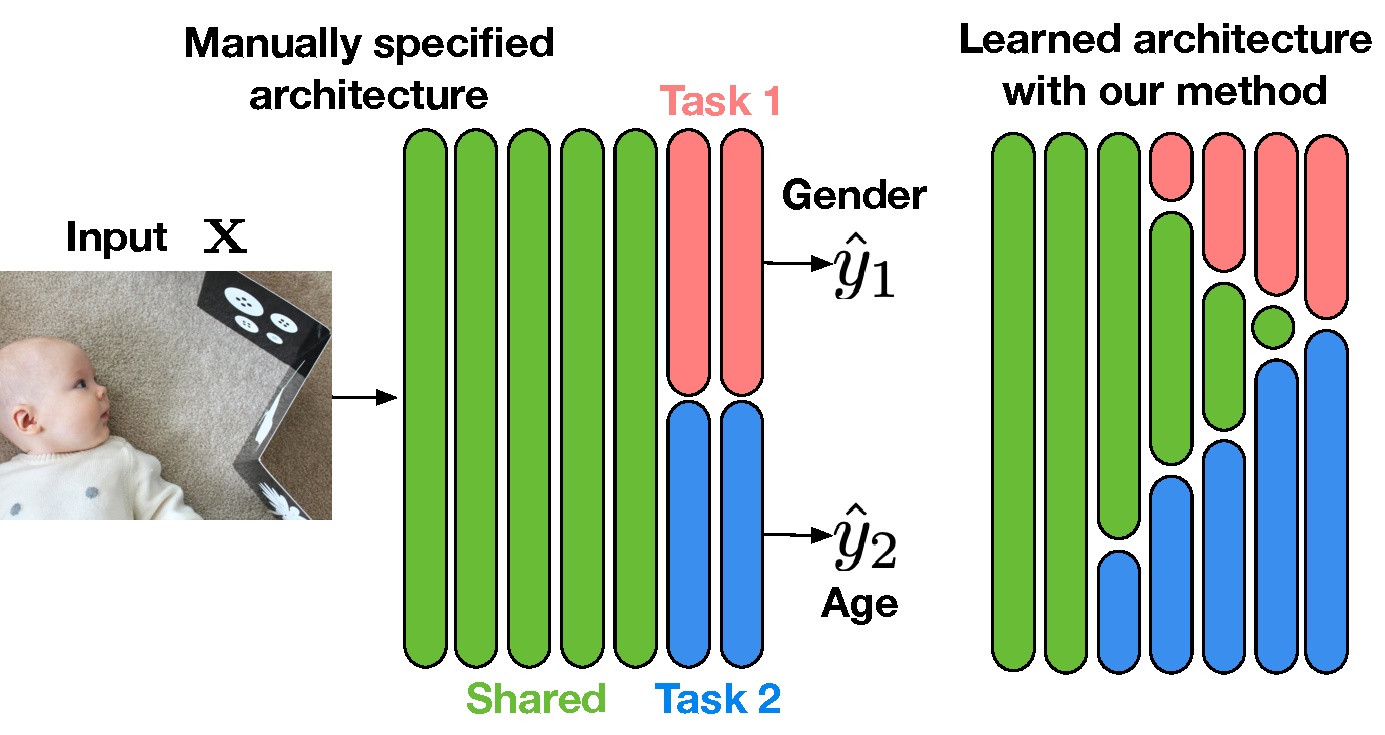
\includegraphics[width=0.7\textwidth]{chapter_6/figures/intro_2.pdf}
\caption{\small Figure on the left illustrates a typical multi-task architecture, while the figure on the right shows an example architecture that can be learned with our method. We propose \emph{Stochastic Filter Groups}, a principled way to learn the assignment of convolution kernels to task-specific and shared groups. }
\label{fig:intro}
\vspace{-4mm}
\end{figure}

A key factor for successful MTL neural network models is the ability to learn shared and task-specific representations \cite{MisraCrossMTL16}. A mechanism to understand the commonalities and differences between tasks allows the model to transfer information between tasks while tailoring the predictive model to describe the distinct characteristics of the individual tasks. The quality of such representations is determined by the architectural design of where model components such as features \cite{Ruder2019SluiceNL} and weights \cite{meyerson2018beyond} are shared and separated between tasks. However, the space of possible architectures is combinatorially large, and the manual exploration of this space is inefficient and subject to human biases. For example, Fig.~\ref{fig:intro} shows a typical CNN architecture for MTL comprised of a shared ``trunk'' feature extractor and task-specific ``branch'' networks \cite{tanno2018autodvt,huang2015cross,jou2016deep,kendall2017multi,ranjan2019hyperface, bragman2018multi}. The desired amount of shared and task-specific representations, and their interactions within the architecture are dependent on the difficulty of the individual tasks and the relation between them, neither of which are a priori known in most cases \cite{taskonomy2018}. This illustrates the challenge of handcrafting an appropriate architecture, and the need for an effective automatic method to learn it from data. 

% the space of such possible branching architectures is combinatorially large and current ap- proaches largely make a decision based on limited manual exploration of this space, often biased by designer’s perception of the relationship among different tasks [25]. Finding a data-driven approach to replace the manual exploration is an important and interesting academic question that has only been sparsely explored.

%  (version 2019-03-19)
% Representation learning forms the basis of multi-task learning. The success of multi-task learning algorithms is generally due to inductive bias \cite{caruana}, which is the process of generating model hypotheses that generalise well across tasks. This generalisation is often the result of sharing the statistical strength of multiple signals and capturing distinct representations that explain underlying factors. In effect, subsets of these representations may be task-specific or task-invariant and can effectively act as strong priors for completely new tasks \cite{lacost2018}. Disentangling subsets of features that are specific, invariant or structured during the learning process can lead to an improvement in model performance \cite{ioannou2017deep} whilst the learned subsets can be exploited in the context of transfer learning \cite{lacost2018} and continual learning \cite{zenke2017}.

% Multi-task learning (MTL) broadly encompasses other learning paradigms such as transfer learning and and sequential learning. In the former, Lacost et al. \cite{lacost2018} learned a prior over various models and demonstrated its potential for few shot-learning on new tasks whilst Kirkpatrick et al. \cite{ewc} explored the concept of sequential learning without forgetting prior tasks. Multi-task learning has proven popular in a wide-range of domains such as in computer vision [\textbf{refs}], natural language processing [\textbf{refs}], medical image computing \cite{bragman2018multi} [\textbf{refs}]. An important foundation of the success of MTL is attributed to the inbuilt sharing mechanism of multi-task architectures. This enables MTL systems to learn shared and generalisable representations, which can lead to improved performance across semantic segmentation [\textbf{ref}], image regression [\textbf{ref}] and object detection [\textbf{ref}] tasks.

%\textbf{This paragraph can be shortened - probably just need a shorter introduction to what is commonly done and the next section in related work can look at soft-parameter sharing, architecture learning algorithms in more detail??}

% Most methods MTL methods can be classified as hard-parameter sharing and soft-parameter sharing algorithms. In the former, the network architecture is composed of a representation network that shares weights across tasks. This branches out to task-specific networks that lead to respective predictions and losses. These methods learn a set of rich, contextual features using domain knowledge from the tasks. The main challenge relates to optimising the multi-task objective function and determining optimal weights \cite{bragman2018multi, gradnorm2018, kendall2017multi}. 

% In soft-parameter sharing, each task has its own model with individual layers of task-specific parameters. The main goal lies in the construction of a mechanism that allows communication across networks. This is can be performed by learning how to share features across the network \cite{meyerson2018beyond, MisraCrossMTL16, xiao2016learning, Kang2011, Yang2017, Ruder2019SluiceNL}, performing clustering of tasks to determine weight sharing \cite{jacob2009, xue2007} or through meta-learning of multi-task architectures \cite{meta}. 

In this paper, we propose \textit{Stochastic Filter Groups} (SFGs); a probabilistic mechanism to learn the amount of task-specific and shared representations needed in each layer of MTL architectures (Fig.~\ref{fig:intro}). Specifically, the SFGs learns to allocate kernels in each convolution layer into either ``specialist'' groups or a ``shared'' trunk, which are specific to or shared across different tasks, respectively (Fig.~\ref{fig:sfg}). The SFG equips the network with a mechanism to learn inter-layer connectivity and thus the structures of task-specific and shared representations. We cast the learning of SFG modules as a variational inference problem.
%, and are thus more susceptible to ``mixing'' of these features. 

We evaluate the efficacy of SFGs on a variety of tasks. In particular, we focus on two multi-task learning problems: 1) age regression and gender classification from face images on UTKFace dataset \cite{zhifei2017cvpr} and 2) semantic regression (i.e. image synthesis) and semantic segmentation on a real-world medical imaging dataset, both of which require predictions over all pixels. Experiments show that our method achieves considerably higher prediction accuracy than baselines with no mechanism to learn connectivity structures, and either higher or comparable performance than a cross-stitch network \cite{MisraCrossMTL16}, while being able to learn meaningful architectures automatically.



%Learning representations is important. Multi-task learning depends on learning good representations that extend to multiple tasks and blabla.

%\begin{enumerate}
%    \item Start of by talking about how learning good representations is important for many aspects of machine learning, from single taask, to multi-task to transfer learning
%    \item Mention importance of multi-task learning and vaguely why it works, what assumptions it is based on
%    \item Talk about ideal world of multi-task framework
%    \item Wrap up introduction of common weaknesses of MT learning algorithm and maybe introduce different taxonomies of algorithms %and what they do
% \end{enumerate}


%\begin{enumerate}
%	\item Learn optimal multi-task network architecture given: a) baseline architecture (VGG, ResNet, HighResNet, UNet) and b) task (age/gender prediction, CT synthesis and segmentation, depth perception and semantic segmentation etc.) 
%    \item Disentangle task-specific and task-invariant features/kernels as a by-product of learning how to share features/propagate information in the network
%    \item Estimate uncertainty in the multi-task network architecture and enable sampling from the architecture-posterior
%\end{enumerate}

%\begin{enumerate}
%    \item Introduction to main problem
%    \item Introduction of various ways of doing, cite some work and describe in very little detail examplars of that work. 
%    \item Describe where our method fits in with this and describe in more detail how it is different than Cross-Stitch
%\end{enumerate}


\section{Related works}
\vspace{-2mm}
Our work is concerned with the goal of learning where to share neural network components across different tasks to maximise the benefit of MTL. The main challenge of such methods lies in designing a mechanism that determines how and where to share weights within the network. There are broadly two categories of methods that determine the nature of weight sharing in MTL networks.

The first category is composed of methods that directly optimise the sharing of weights in order to maximise task-wise performance. These methods set out to learn a set a vectors that control which features are shared within a layer and how these are distributed across \cite{long2017learning, meyerson2018beyond, MisraCrossMTL16, Ruder2019SluiceNL}. They start with a baseline CNN architecture where they learn additional connections and pathways that define the final MTL model. For instance, Cross-Stitch networks \cite{MisraCrossMTL16} control the degree of weight sharing at each convolution layer whilst Soft-Layer Ordering \cite{meyerson2018beyond} goes beyond the assumption of parallel ordering of feature hierarchies to allow features to mix at different layers depending on the task. In contrast, the second group of MTL methods focuses on weight clustering based on task-similarity \cite{xue2007multi, jacob2009, Kang2011,lu2017fully,mejjati2018multi}. For example, \cite{lu2017fully} employed a greedy, iterative algorithm to grow a tree-like deep architecture that clusters similar tasks hierarchically or \cite{mejjati2018multi} which determines the degree of weight sharing based on statistical dependency between tasks.

Our method falls into first category, and differentiates itself by performing ``hard' partitioning of task-specific and shared features. By contrast, prior methods are based on ``soft'' sharing of features \cite{MisraCrossMTL16,Ruder2019SluiceNL} or weights \cite{long2017learning,meyerson2018beyond}. These methods generally learn a set of mixing coefficients that determine the weighted sum of features throughout the network, which does not impose connectivity structures on the architecture. On the other hand, our method learns a distribution over the connectivity of layers by grouping kernels. This allows our model to learn meaningful grouping of task-specific and shared features as illustrated in Fig.~\ref{fig:activations}. 

%This relates to the work of Ioannou et al. \cite{ioannou2017deep}. It was shown that enforcing structure and connectivity in single task networks through Filter Groups could lead to better performance in addition structured representations. Our work enables this process 


%These methods generally learn a set of mixing coefficients that determines the weighted sum of features throughout the network. However, this is not always likely to lead to meaningful representations. 





%the paper proposes to learn a soft orderingover a set of layers for multitask learning (MTL)i.e. at every step of the forward propagation, each task is free to choose its unique soft (‘convex’)combination of the outputs from all available layers. 

%Previous works defines its sharing mechanism as a linear summation of activations \cite{MisraCrossMTL16,Ruder2019SluiceNL}, through placing a tensor normal prior on weights that are shared  \cite{long2017learning} or by applying soft ordering of shared layers \cite{meyerson2018beyond}



% \paragraph{Comparison with Cross-Stitch:}
% Cross-stitch provides 
% Our method differs from cross-stitch proposed in \cite{MisraCrossMTL16} in some crucial ways: 
% \begin{itemize}
%     \item end-to-end training 
%     \item we learn connectivity structures between layers, but cross-stitch only how to combine 
%     \items filter groups showed that enforcing prior connectivity in the network both improved results but also led to structured representations. Our network directly learns the connectivity/structure representations in an optimal way. In contrast, cross-stitch learns how to combine feature activations across network depth with unbounded mixing coefficients which doesn't guarantee any meaningful structure. 
    
% \end{itemize}







% The underlying theme for weight sharing in MTL can generally be stratified into two sets of work. In the first, the main goal lies in the construction of a mechanism that allows communication across the network. The second concerns techniques that control the sharing of weight vectors by clustering related weights by on task similarity.  


%Methods that aim to figure out how to share weight vectors by clustering related weights together and use them for multi-task learning.
%\begin{enumerate}
%    \item Clustered multi-task learning: a convex formulation \cite{jacob2009}. 
%    \item Maximizing statistical dependence: \cite{mejjati2018multi}
%    \item Clustering similar tasks:\cite{xue2007multi}, there is also prior work by Zoubin Gharamani on this subject. 
%    \item Grouping structures \cite{Kang2011}
%\end{enumerate}
%performing clustering of tasks to determine weight sharing \cite{jacob2009, xue2007} or through meta-learning of multi-task architectures \cite{meta}. 

%Ruder, 2017 \cite{ruder2017overview} provides a comprehensive review of other categories of multi-task learning methods in neural networks in greater details. 






% \begin{enumerate}
%     \item Task weights as homoscedastic task uncertainty \cite{kendall2017multi}. Task weights are modelled as homoscedastic uncertainty which follow from the probabilistic interpretation of the likelihood functions.
%     \item Task weighting with heterscedastic uncertainty \cite{bragman2018multi}. I think we know this one.
%     \item Gradient normalisation for adaptive loss balancing \cite{gradnorm2018}. Dynamic tuning of gradient magnitudes to automatically balance training in deep multitask models. Assumption is that in linear sum multi-task losses, if backpropagated gradient of task loss is large relative to others, tasks do not learn at similar rates and thus optimal performance cannot be achieved.
%     \item Naive sum of per task losses in UberNet \cite{ubernet2017}
%     \item Adversarial loss: \cite{liu2018multi}
% \end{enumerate}


% \subsection{Multi-task via architectural optimisation}
% The main goal lies in the construction of a mechanism that allows communication across networks. This is can be performed by learning how to share features across the network \cite{meyerson2018beyond, MisraCrossMTL16, xiao2016learning, Kang2011, Ruder2019SluiceNL}, 

% \textcolor{black}{Need to cite more classic literature on MTL with graphical models.}
% \begin{enumerate}
%     \item Learning relationships between tasks: ``Taskonomy'', \cite{taskonomy2018}. Discovering hierarchical relationships between tasks. \textcolor{black}{(Ryu): need to understand how transfer learning can be do based on the learned taskonomy.}
%     \item Learning when to share features/layers between tasks:
%         \begin{itemize}
%             \item ``Cross-Stitch Networks'' \cite{MisraCrossMTL16}
%             \item Soft-layer Ordering \cite{meyerson2018beyond}: Soft-layer Ordering \cite{meyerson2018beyond}: the paper proposes to learn a soft ordering over a set of layers for multitask learning (MTL) i.e. at every step of the forward propagation, each task is free to choose its unique soft (`convex') combination of the outputs from all available layers. Such soft combination is learned jointly with the tasks. 
%             \item Deep Relationship Networks \cite{long2017learning}: Hard-parameter set-up but with soft-parameter sharing in fully connected layers of the network. They place matrix priors on the fully connected layers to learn relationship between tasks. Tensor normal distribution prior on weights  normal distribution with decomposable covariance MAP estimate of network weights in fully connected layers. Likelihood in posterior is modelled by the CNN conv layers. Prior is supposed to model the relationship across parameter tenors  covariances model: relationship between features, classes and weights across layers.
%             \item Sluice Network \cite{Ruder2019SluiceNL}
%             \item Fully-Adaptive Feature Sharing \cite{lu2017fully}
%         \end{itemize}
        
%     \item Disentangling representations:
%     \begin{itemize}
%         \item Domain specific disentanglement: Domain Separation Network for domain adaptation \cite{bousmalis2016domain}, Domain Guided Dropout \cite{xiao2016learning} for multi-domain learning task. 
        
%         \item Generative models: \cite{kim2018disentangling} 
%     \end{itemize}
% \end{enumerate}

%%% DEEP RELATIONSHIP NETWORKS - NIPS 2017
\section{Methods}
We introduce a new approach for determining where to learn task-specific and shared representation in multi-task CNN architectures. We propose \textit{stochastic filter groups} (SFG), a probabilistic mechanism to partition kernels in each convolution layer into ``specialist" groups or a ``shared" group, which are specific to or shared across different tasks, respectively. We employ variational inference to learn the distributions over the possible grouping of kernels and network parameters that determines the connectivity between layers and the shared and task-specific features. This naturally results in a learning algorithm that optimally allocate representation capacity across multi-tasks via gradient-based stochastic optimization, e.g. stochastic gradient descent. 

% Typically, there is significant human bias in the design of multi-task architectures. Generally, hard-parameter sharing or soft-parameter sharing is chosen followed by various engineering implementations designed to help regularise network weights across tasks, the degree of sharing of weights and the parallel ordering of layers. 

\begin{figure}[ht]
	\center
% 	\vspace{-3mm}
	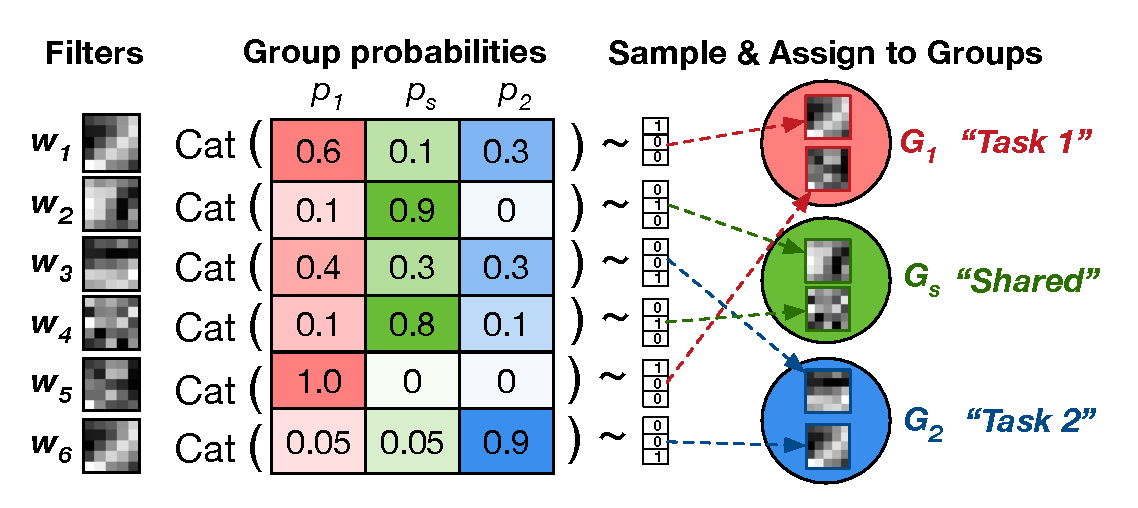
\includegraphics[width=0.85\linewidth]{chapter_6/figures/sfg_figure_02.pdf}
	\caption{\small Illustration of filter assignment in a SFG module. Each kernel $\{\mathbf{w}_{k}\}$ in the given convolution layer is probabilistically assigned to one of the filter groups $G_1, G_{s}, G_{2}$ according to the sample drawn from the associated categorical distribution $\text{Cat}(p_1, p_{s}, p_2)$. }
    \label{fig:sfg}
\end{figure}

\begin{figure}[ht]
	\center
	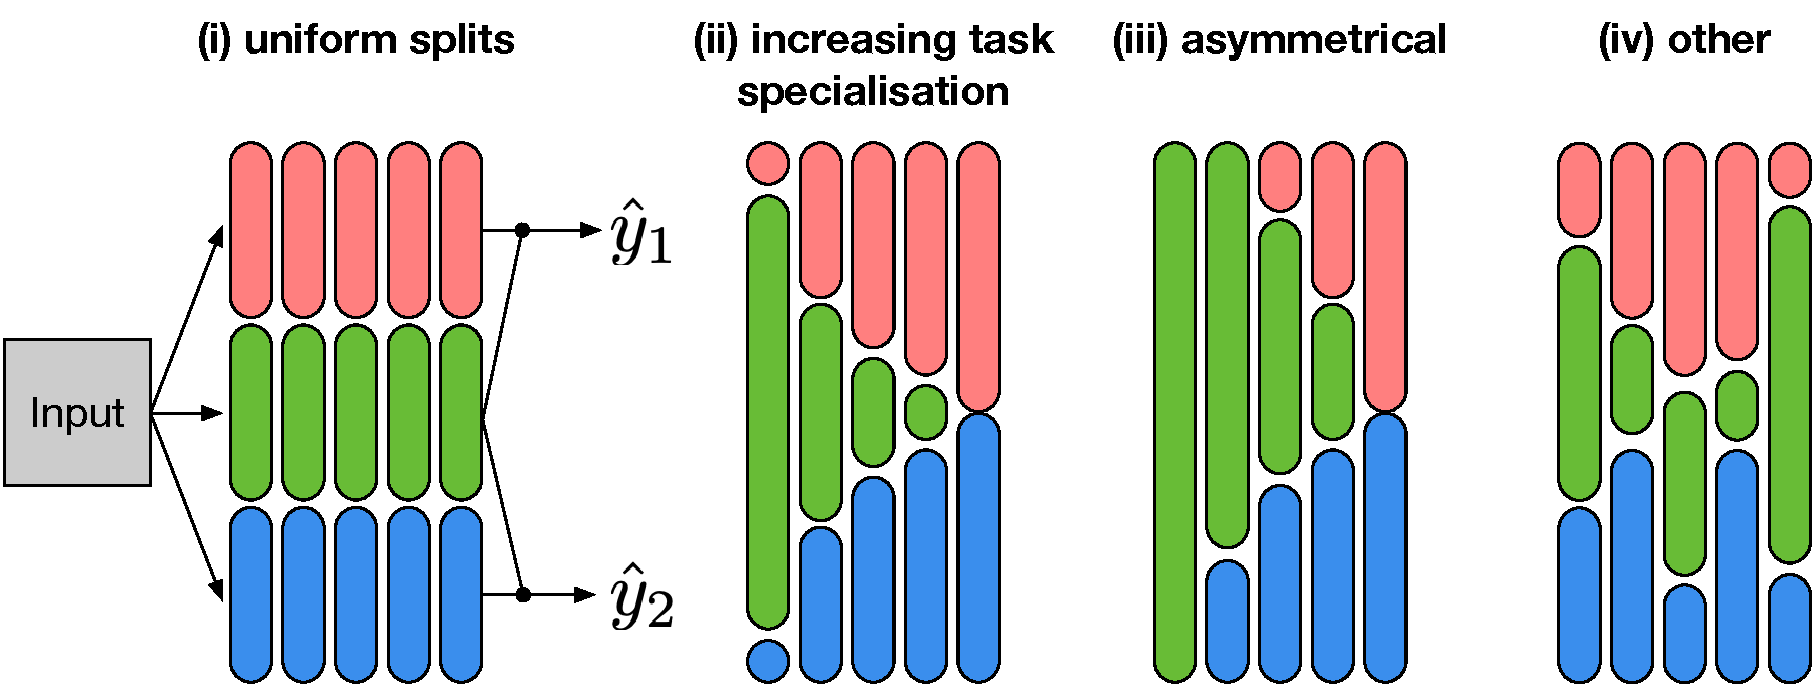
\includegraphics[width=0.9\linewidth]{chapter_6/figures/example_nets_03.pdf}
	\caption{\small Illustration of possible grouping patterns learnable with the proposed method. Each set of green, pink and yellow blocks represent the ratio of filter groups $G_1$ (red), $G_{s}$ (green) and $G_{2}$ (blue). (i) denotes the case where all kernels are uniformly split. (ii) \& (iii) are the cases where the convolution kernels become more task-specific at deeper layers. (iv) shows an example with more heterogeneous splits across tasks.}
    \label{fig:different_grouping}
\end{figure}

\begin{figure}[ht]
	\center
% 	\vspace{-3mm}
	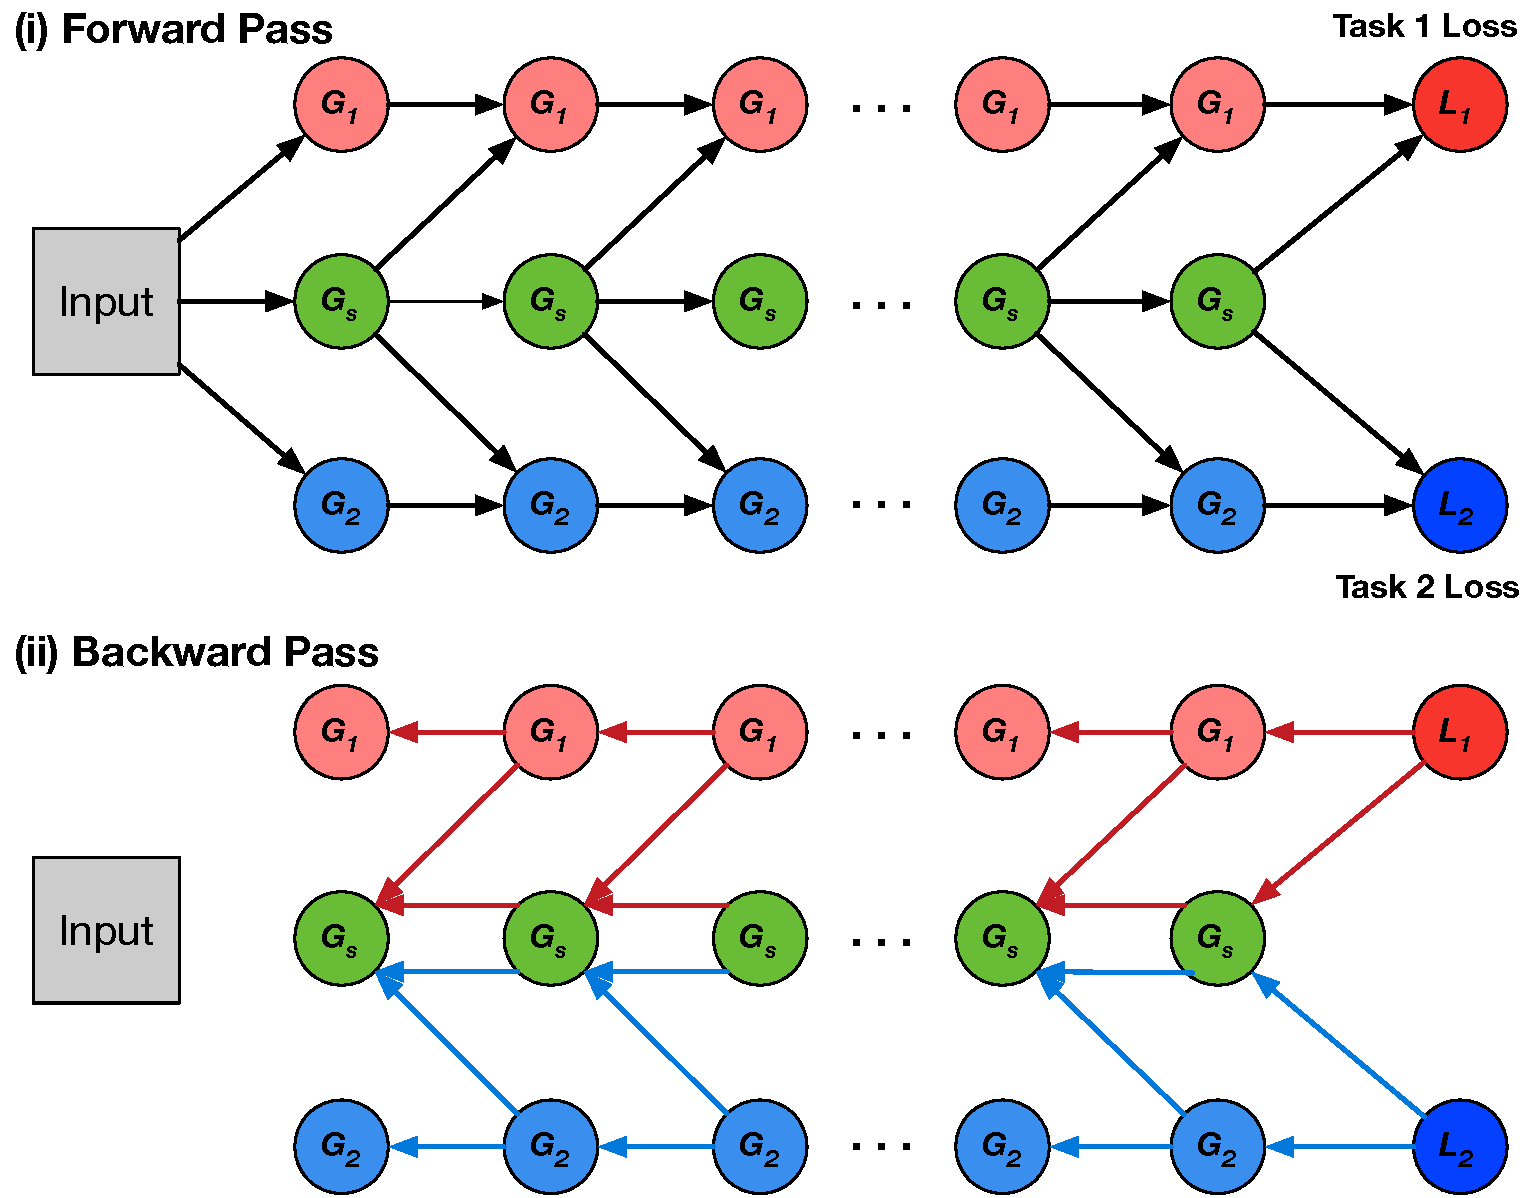
\includegraphics[width=0.75\linewidth]{chapter_6/figures/forward_and_backward.pdf}
	\caption{\small Illustration of feature routing. The circles $G_{1}, G_{s}, G_{2}$ denote the task-specific and shared filter groups in each layer. (i) shows the directions of routing of activations between different filter groups while (ii) shows the directions of the gradient flow from the task losses $L_{1}$ and $L_{2}$. The red and blue arrows denote the gradients that step from $L_{1}$ and $L_{2}$, respectively. The task-specific groups $G_{1}, G_{2}$ are only updated based on the associated losses, while the shared group $G_{s}$ is updated based on both. }
    \label{fig:forward_and_backward}
\end{figure}

\begin{figure*}[ht]

% 	\vspace{-3mm}
    %\hspace{0.075\linewidth}
    \center
	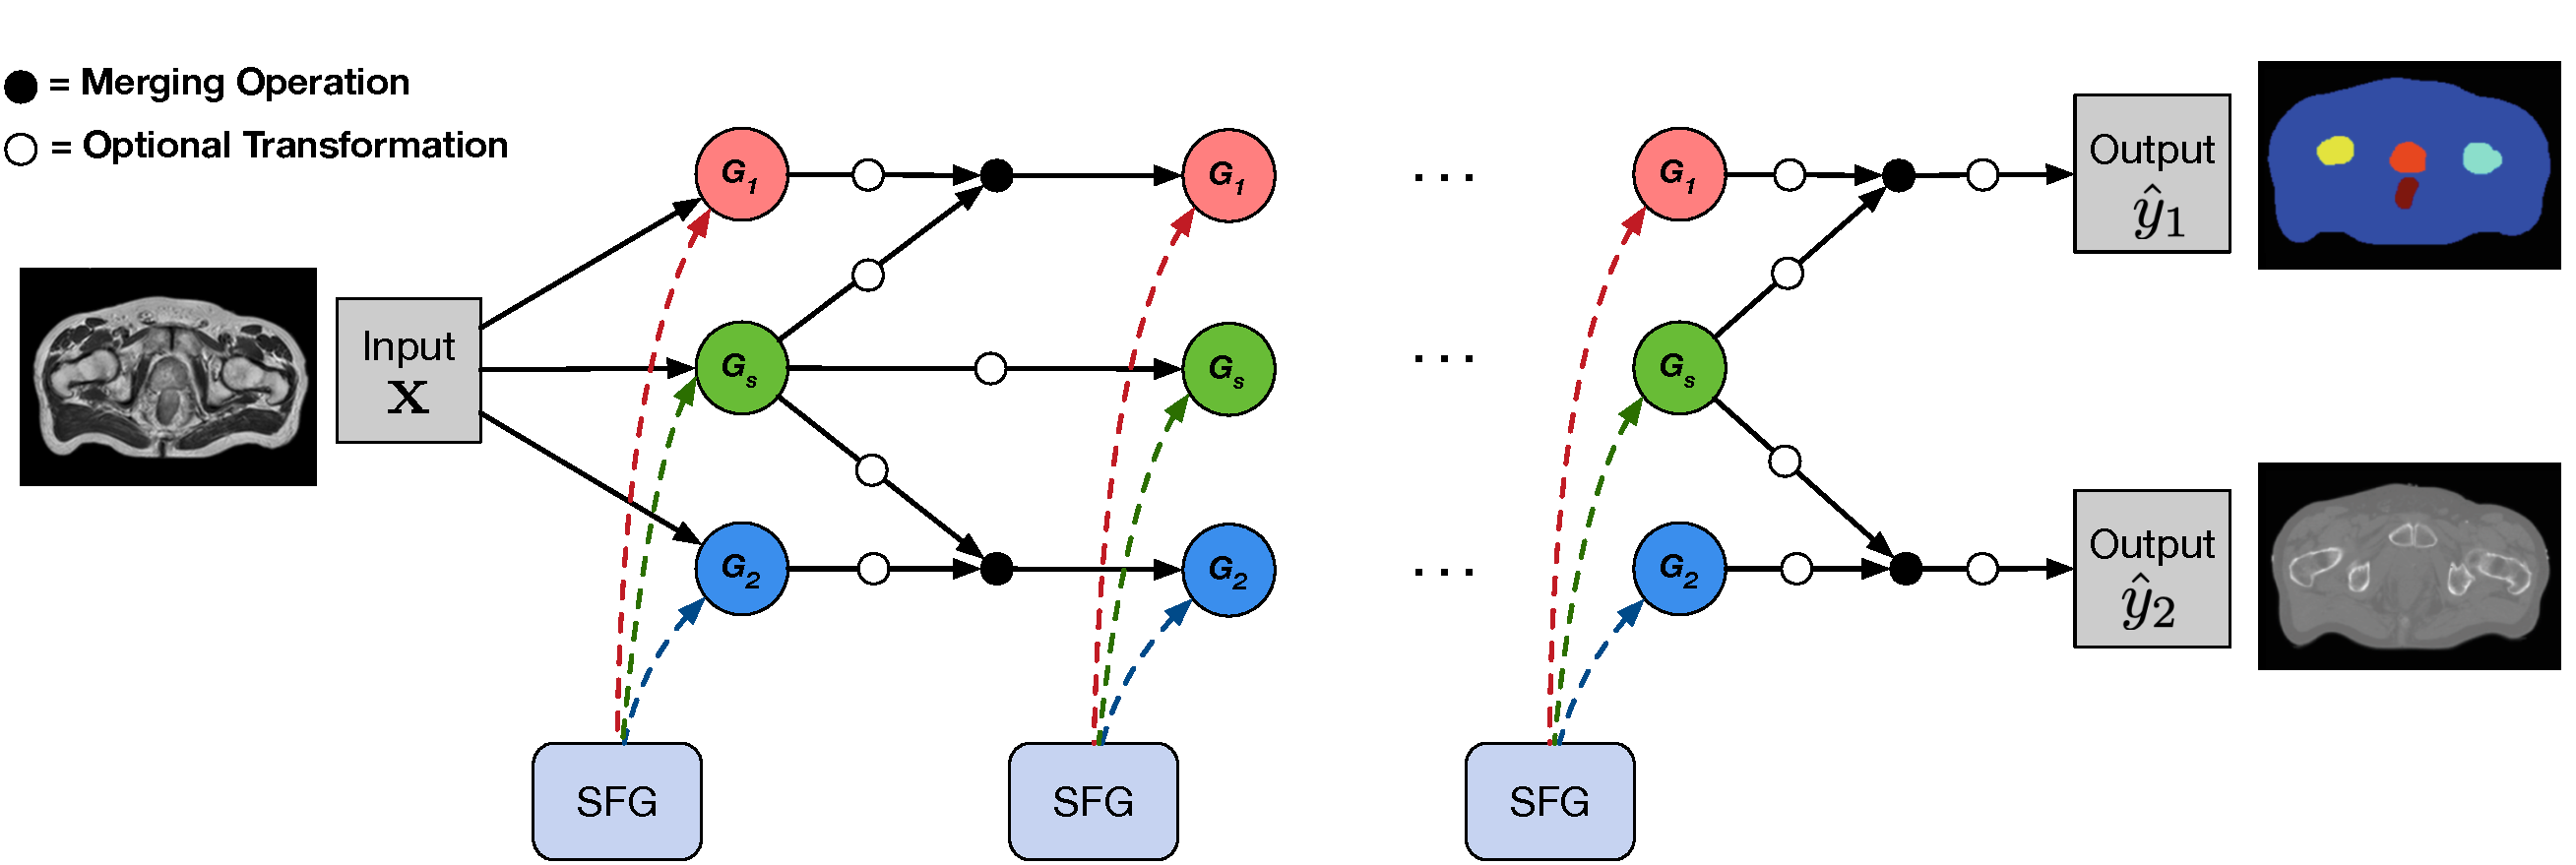
\includegraphics[width=\linewidth]{chapter_6/figures/schematic_03.pdf}
	\caption{\small Schematic of the proposed multi-task architecture based on a series of SFG modules in the presence of two tasks. At each convolution layer, kernels are stochastically assigned to task-specific and shared filter groups $G_{1}, G_{s}, G_{2}$. Each input image is first convolved with the respective filter groups to yield three distinct sets of output activations, which are routed sparsely to the filter groups in the second layer layer. This process repeats in the remaining SFG modules in the architecture until the last layer where the outputs of the final SFG module are combined into task-specific predictions $\hat{y}_{1}$ and $\hat{y}_{2}$. Each small white circle denotes an optional transformation (e.g. extra convolutions) and black circle merges the incoming inputs (e.g. concatenation).}
    \label{fig:schematic}
\end{figure*}

% \textcolor{black}{(Ryu): a very rough summary of what Felix and I previously discussed. For each convolution kernel, the model learns a categorical distribution to separate/share representations across tasks. In the case of 2 tasks (e.g. synthesis and segmentation), the distribution is over three classes i.e. "task 1", "task 2" and "common". An apparent drawback of this approach is the fact that the number of possible combinations is of factorial order in the number of tasks. The parameters of the categorial distribution could be learned via variational inference in a similar manner to how dropout rates are learned in the Concrete Dropout paper \href{https://arxiv.org/abs/1705.07832}{(link)}. In other words, learning the probabilistic separation/sharing of architectures could be potentially achieved with a multi-way extension of Concrete dropout. Appropriate prior need to be defined on the parameters of categorial (e.g. Dirichlet distributions) so the inference is tractalble}. 

% stochastic hard separation. 
\subsection{Stochastic Filter Groups}
SFGs introduce a sparse connection structure into the architecture of CNN for multi-task learning in order to separate features into task-specific and shared components. Ioannou et al. \cite{ioannou2017deep} introduced \textit{filter groups} to partition kernels in each convolution layer into groups, each of which acts only on a subset of the preceding features, and demonstrated that such sparsity reduces computational cost and number of parameters without compromising accuracy. Here we adapt the concept of filter groups to the multi-task learning paradigm and propose an extension with an additional mechanism for learning an optimal kernel grouping rather than pre-specifying them.

For simplicity, we describe SFGs for the case of multitask learning with two tasks, but can be trivially extended to a larger number of tasks. At the $l^{\text{th}}$ convolution layer in a CNN architecture with $K_l$ kernels $\{\mathbf{w}^{(l),k}\}^{K_l}_{k=1}$, the associated SFG performs two operations: 

\begin{enumerate}
    \item \textbf{Filter Assignment:} each kernel $\mathbf{w}_{k}^{(l)}$ is stochastically assigned to either: i) the ``task-1 specific group'' $G^{(l)}_{1}$, ii) ``shared group'' $G^{(l)}_{s}$ or iii) ``task-2 specific group'' $G^{(l)}_{2}$ with respective probabilities $\mathbf{p}^{(l),k} = [p^{(l),k}_1, p^{(l),k}_{s}, p^{(l),k}_2] \in [0,1]^3$. Convolving with the respecitve filter groups yields distinct sets of features $F^{(l)}_1, F^{(l)}_{s}, F^{(l)}_{2}$. Fig.~\ref{fig:sfg} illustrates this operation and Fig.~\ref{fig:different_grouping} shows different learnable patterns. 
    % $\{(p_1, p_2, p_3):\sum_{i}p_i = 1,  p_i\geq 0 \forall i=1,2,3\}$
    
    \item \textbf{Feature Routing:} as shown in Fig.~\ref{fig:forward_and_backward}~(i), the features $F^{(l)}_1, F^{(l)}_{s}, F^{(l)}_{2}$ are routed to the filter groups $G_{1}^{(l+1)}, G_{s}^{(l+1)}, G_{2}^{(l+1)}$ in the subsequent $(l+1)^{\text{th}}$ layer in such a way to respect the task-specificity and sharedness of filter groups in the $l^{\text{th}}$ layer. Specifically, we perform the following routing for $l>0$: 
        \begin{align*}
        F^{(l+1)}_1 &= h^{(l+1)}\big{(}[F^{(l)}_1|F^{(l)}_{s}]*G^{(l+1)}_{1}\big{)}\\ 
        F^{(l+1)}_{s} &= h^{(l+1)}\big{(} F^{(l)}_{s}*G^{(l+1)}_{s}\big{)}\\ 
        F^{(l+1)}_2 &= h^{(l+1)}\big{(}[F^{(l)}_2|F^{(l)}_{s}]*G^{(l+1)}_{2}\big{)}
        \end{align*}
    where each $h^{(l+1)}$ defines the choice of non-linear function, $*$ denotes convolution operation and $|$ denotes a merging operation of arrays (e.g. concatenation). At $l=0$, input image $\mathbf{x}$ is simply convolved with the first set of filter groups to yield $F^{(1)}_{i} = h^{(1)}\big{(}\mathbf{x}*G^{(1)}_{i}\big{)}, i\in\{1,2,s\}$. Fig.~\ref{fig:forward_and_backward}(ii) shows that such sparse connectivity ensures the parameters of $G^{(l)}_{1}$ and $G^{(l)}_{2}$ are only learned based on the respective task losses, while $G^{(l)}_{s}$ is optimised based on both tasks. 
\end{enumerate}
    
    
Fig.~\ref{fig:schematic} provides a schematic of our overall architecture, in which each SFG module stochastically generates filter groups in each convolution layer and the resultant features are sparsely routed as described above. The merging modules, denoted as black circles, combine the task-specific and shared features appropriately, i.e. $[F^{(l)}_{i}|F^{(l)}_{s}], i = 1,2$ and pass them to the filter groups in the next layer. Each white circle denotes the presence of additional transformations  (e.g. convolutions or fully connected layers) in each $h^{(l+1)}$, performed on top of the standard non-linearity (e.g. ReLU). 

    
The proposed sparse connectivity is integral to ensure task performance and structured representations. In particular, one might argue that the routing of ``shared'' features $F^{(l)}_{s}$ to the respective ``task-specific'' filter groups $G^{(l+1)}_{1}$ and $G^{(l+1)}_{2}$ is not necessary to ensure the separation of gradients across the task losses. However, this connection allows for learning more complex task-specific features at deeper layers in the network. For example, without this routing, having a large proportion of ``shared'' filter group $G_{s}$ at the first layer (Fig.~\ref{fig:different_grouping}~(ii)) substantially reduces the amount of features available for learning task-specific kernels in the subsequent layers---in the extreme case in which all kernels in one layer are assigned to $G_{s}$, the task-specific filter groups in the subsequent layers are effectively unused. 

Another important aspect that needs to be highlighted is the varying dimensionality of feature maps. Specifically, the number of kernels in the respective filter groups $G^{(l)}_{1}, G^{(l)}_{s}, G^{(l)}_{2}$ can vary at each iteration of the training, and thus, so does the depth of the resultant feature maps $F^{(l)}_{1}, F^{(l)}_{s}, F^{(l)}_{2}$. Instead of directly working with features maps of varying size, we implement the proposed architecture by defining $F^{(l)}_{1}, F^{(l)}_{s}, F^{(l)}_{2}$ as sparse tensors. At each SFG module, we first convolve the input features with all kernels, and generate the output features from each filter group by zeroing out the channels that root from the kernels in the other groups, resulting in $F^{(l)}_{1}, F^{(l)}_{s}, F^{(l)}_{2}$ that are sparse at non-overlapping channel indices. In the simplest form with no additional transformation (i.e. the grey circles in Fig.~\ref{fig:schematic} are identity functions), we define the merging operation $[F^{(l)}_{i}|F^{(l)}_{s}], i = 1,2$ as pixel-wise summation. In the presence of more complex transforms (e.g. residual blocks), we concatenate the output features in the channel-axis and perform a 1x1 convolution to ensure the number of channels in $[F^{(l)}_{i}|F^{(l)}_{s}]$ is the same as in $F^{(l)}_{s}$. 


\subsection{T+1 Way ``Drop-Out''}
Here we derive the method for simultaneously optimising the CNN parameters and grouping probabilities. We achieve this by extending the variational interpretation of binary dropout \cite{gal2016uncertainty,gal2017concrete} to the $(T+1)$-way assignment of each convolution kernel to the filter groups where $T$ is the number of tasks. As before, we consider the case $T=2$. 

Suppose that the architecture consists of $L$ SFG modules, each with $K_l$ kernels where $l$ is the index. As the posterior distribution over the convolution kernels in SFG modules $p(\mathcal{W}|\textbf{X}, \mathbf{Y}^{(1)}, \mathbf{Y}^{(2)})$ is intractable, we approximate it with a simpler distribution $q_{\phi}(\mathcal{W})$ where $\mathcal{W}=\{\mathbf{w}^{(l),k}\}_{k=1,...,K_{l},l=1,...,L}$. Assuming that the posterior distribution factorizes over layers and kernels up to group assignment, we defined the variational distribution as:
\begin{align*}
 q_{\phi}(\mathcal{W}) &= \prod_{l=1}^{L}\prod_{k=1}^{K_{l}} q_{\phi_{lk}}(\mathbf{w}^{(l),k}) \\
 &= \prod_{l=1}^{L}\prod_{k=1}^{K_{l}} q_{\phi_{lk}}(\mathbf{w}^{(l),k}_1,\mathbf{w}^{(l),k}_{s}, \mathbf{w}^{(l),k}_{2})
\end{align*}
where $\{\mathbf{w}^{(l),k}_1,\mathbf{w}^{(l),k}_{s}, \mathbf{w}^{(l),k}_{2}\}$ denotes the $k^{\text{th}}$ kernel in $l^{\text{th}}$ convolution layer after being routed into task-specific $G^{(l)}_1, G^{(l)}_2$ and shared group $G^{(l)}_{s}$. We define each $q_{\phi_{lk}}(\mathbf{w}^{(l),k}_1,\mathbf{w}^{(l),k}_2, \mathbf{w}^{(l),k}_{s})$ as: 
\begin{align}
\mathbf{w}^{(l),k}_{i} &= z^{(l),k}_{i}\cdot\mathbf{w}^{(l),k}\, \,\,\text{for } i \in\{1,s,2\}\\
\mathbf{z}^{(l),k}&=[z^{(l),k}_{1}, z^{(l),k}_{2},  z^{(l),k}_{s}] \sim \text{Cat}(\mathbf{p}^{(l),k}) \label{eq:sample_cat}
\end{align}
where $\mathbf{z}^{(l),k}$ is the one-hot encoding of a sample from the categorical distribution over filter group assignments. The variational parameters $\phi_{lk}$ consists of the pre-grouping convolution kernel $\mathbf{w}^{(l),k}$ and the grouping probabilities $\mathbf{p}^{(l),k}=[p^{(l),k}_1, p^{(l),k}_{s}, p^{(l),k}_2]$. 

We minimize the KL divergence between the approximate posterior $q_{\phi}(\mathcal{W})$ and $p(\mathcal{W}|\textbf{X}, \mathbf{Y}^{(1)}, \mathbf{Y}^{(2)})$. Assuming that the joint likelihood over the two tasks factorizes, we have the following optimization objective:
\begin{multline}\label{eq:variational_loss}
    \mathcal{L}_{\text{MC}}(\phi) = -\frac{N}{M}\sum_{i=1}^{M} \Big{[}\text{log } p(y^{(1)}_i|\mathbf{x}_i, \mathcal{W}_i) + \text{log }p(y^{(2)}_i|\mathbf{x}_i, \mathcal{W}_i)\Big{]} \\ + \sum_{l=1}^{L}\sum_{k=1}^{K_l}\text{KL}(q_{\phi_{lk}}(\mathbf{W}^{(l),k})||p(\mathbf{W}^{(l),k}))
\end{multline}
where $M$ is the size of the mini-batch, $N$ is the total number of training data points, and $\mathcal{W}_i$ denotes a set of model parameters sampled from $q_{\phi}(\mathcal{W})$. The last KL term regularizes the deviation of the approximate posterior from the prior $p(\mathbf{W}^{(l),k})=\mathcal{N}(0, \mathbf{I}/l^{2})$ where $l>0$. Adapting the approximation presented in \cite{gal2016uncertainty} to our scenario, we obtain:
\begin{equation}\label{eq:KL}
    \text{KL}(q_{\phi_{lk}}(\mathbf{C}^{(l),k})||p(\mathbf{C}^{(l),k})) \propto \frac{l^2}{2}||\mathbf{M}^{(l),k}||^{2}
    _{2} - \mathcal{H}(\mathbf{p}^{(l),k})
\end{equation}
where $\mathcal{H}(\mathbf{p}^{(l),k})=-\sum_{i\in \{1,2,s\}}p^{(l),k}_i\text{log }p^{(l),k}_i$ is the entropy of the grouping probabilities. While the first term performs the L2-weight norm, the second term pulls the grouping probabilities towards the uniform distribution. Plugging eq.\eqref{eq:KL} into eq.\eqref{eq:variational_loss} yields the overall loss: 

\begin{multline}\label{eq:total_loss}
\medmuskip=0mu
\thinmuskip=0mu
\thickmuskip=0mu
\mathcal{L}_{\text{MC}}(\phi) = -\frac{N}{M}\sum_{i=1}^{M} \left[\log\text{\,} p\left(y^{(1)}_i|\mathbf{x}_i, \mathcal{W}_i\right) + \log\text{\,} p\left(y^{(2)}_i|\mathbf{x}_i, \mathcal{W}_i\right)\right] \\ + \lambda_{1} \cdot \sum_{l=1}^{L}\sum_{k=1}^{K_l}||\mathbf{w}^{(l),k}||^{2} - \lambda_{2} \cdot \sum_{l=1}^{L}\sum_{k=1}^{K_l}\mathcal{H}(\mathbf{p}^{(l),k})
\end{multline}
where $\lambda_1>0, \lambda_2>0$ are regularization coefficients. 

We note that the discrete sampling operation during filter group assignment (eq.~\eqref{eq:sample_cat}) creates discontinuities, giving the first term in the objective function (eq.~\ref{eq:total_loss}) zero gradient with respect to the grouping probabilities $\{\mathbf{p}^{(l),k}\}$. We therefore, as employed in \cite{kendall2017multi} for the binary case, approximate each of the categorical variables $\text{Cat}(\mathbf{p}^{(l),k})$ by the Gumbel-Softmax distribution, $\text{GSM}(\mathbf{p}^{(l),k}, \tau)$ \cite{maddison2016concrete,jang2016categorical}, a continuous relaxation which allows for sampling, differentiable with respect to the parameters $\mathbf{p}^{(l),k}$ through a reparametrisation trick. The temperature term $\tau$ adjusts the bias-variance tradeoff of gradient approximation; as the value of $\tau$ approaches 0, samples from the GSM distribution become one-hot (i.e. lower bias) while the variance of the gradients increases. \textcolor{black}{In practice, we start at a high $\tau$ and anneal to a small but non-zero value as in \cite{jang2016categorical,gal2017concrete} as detailed in supplementary materials.}

%Stochastic gradient estimators (e.g. REINFORCE, RELAX, REBAR!, etc)


%%%%%%%%% Nice to have the sampling thing, but could be moved into the supp.
% \begin{figure}[ht]
% 	\center
% % 	\vspace{-3mm}
% 	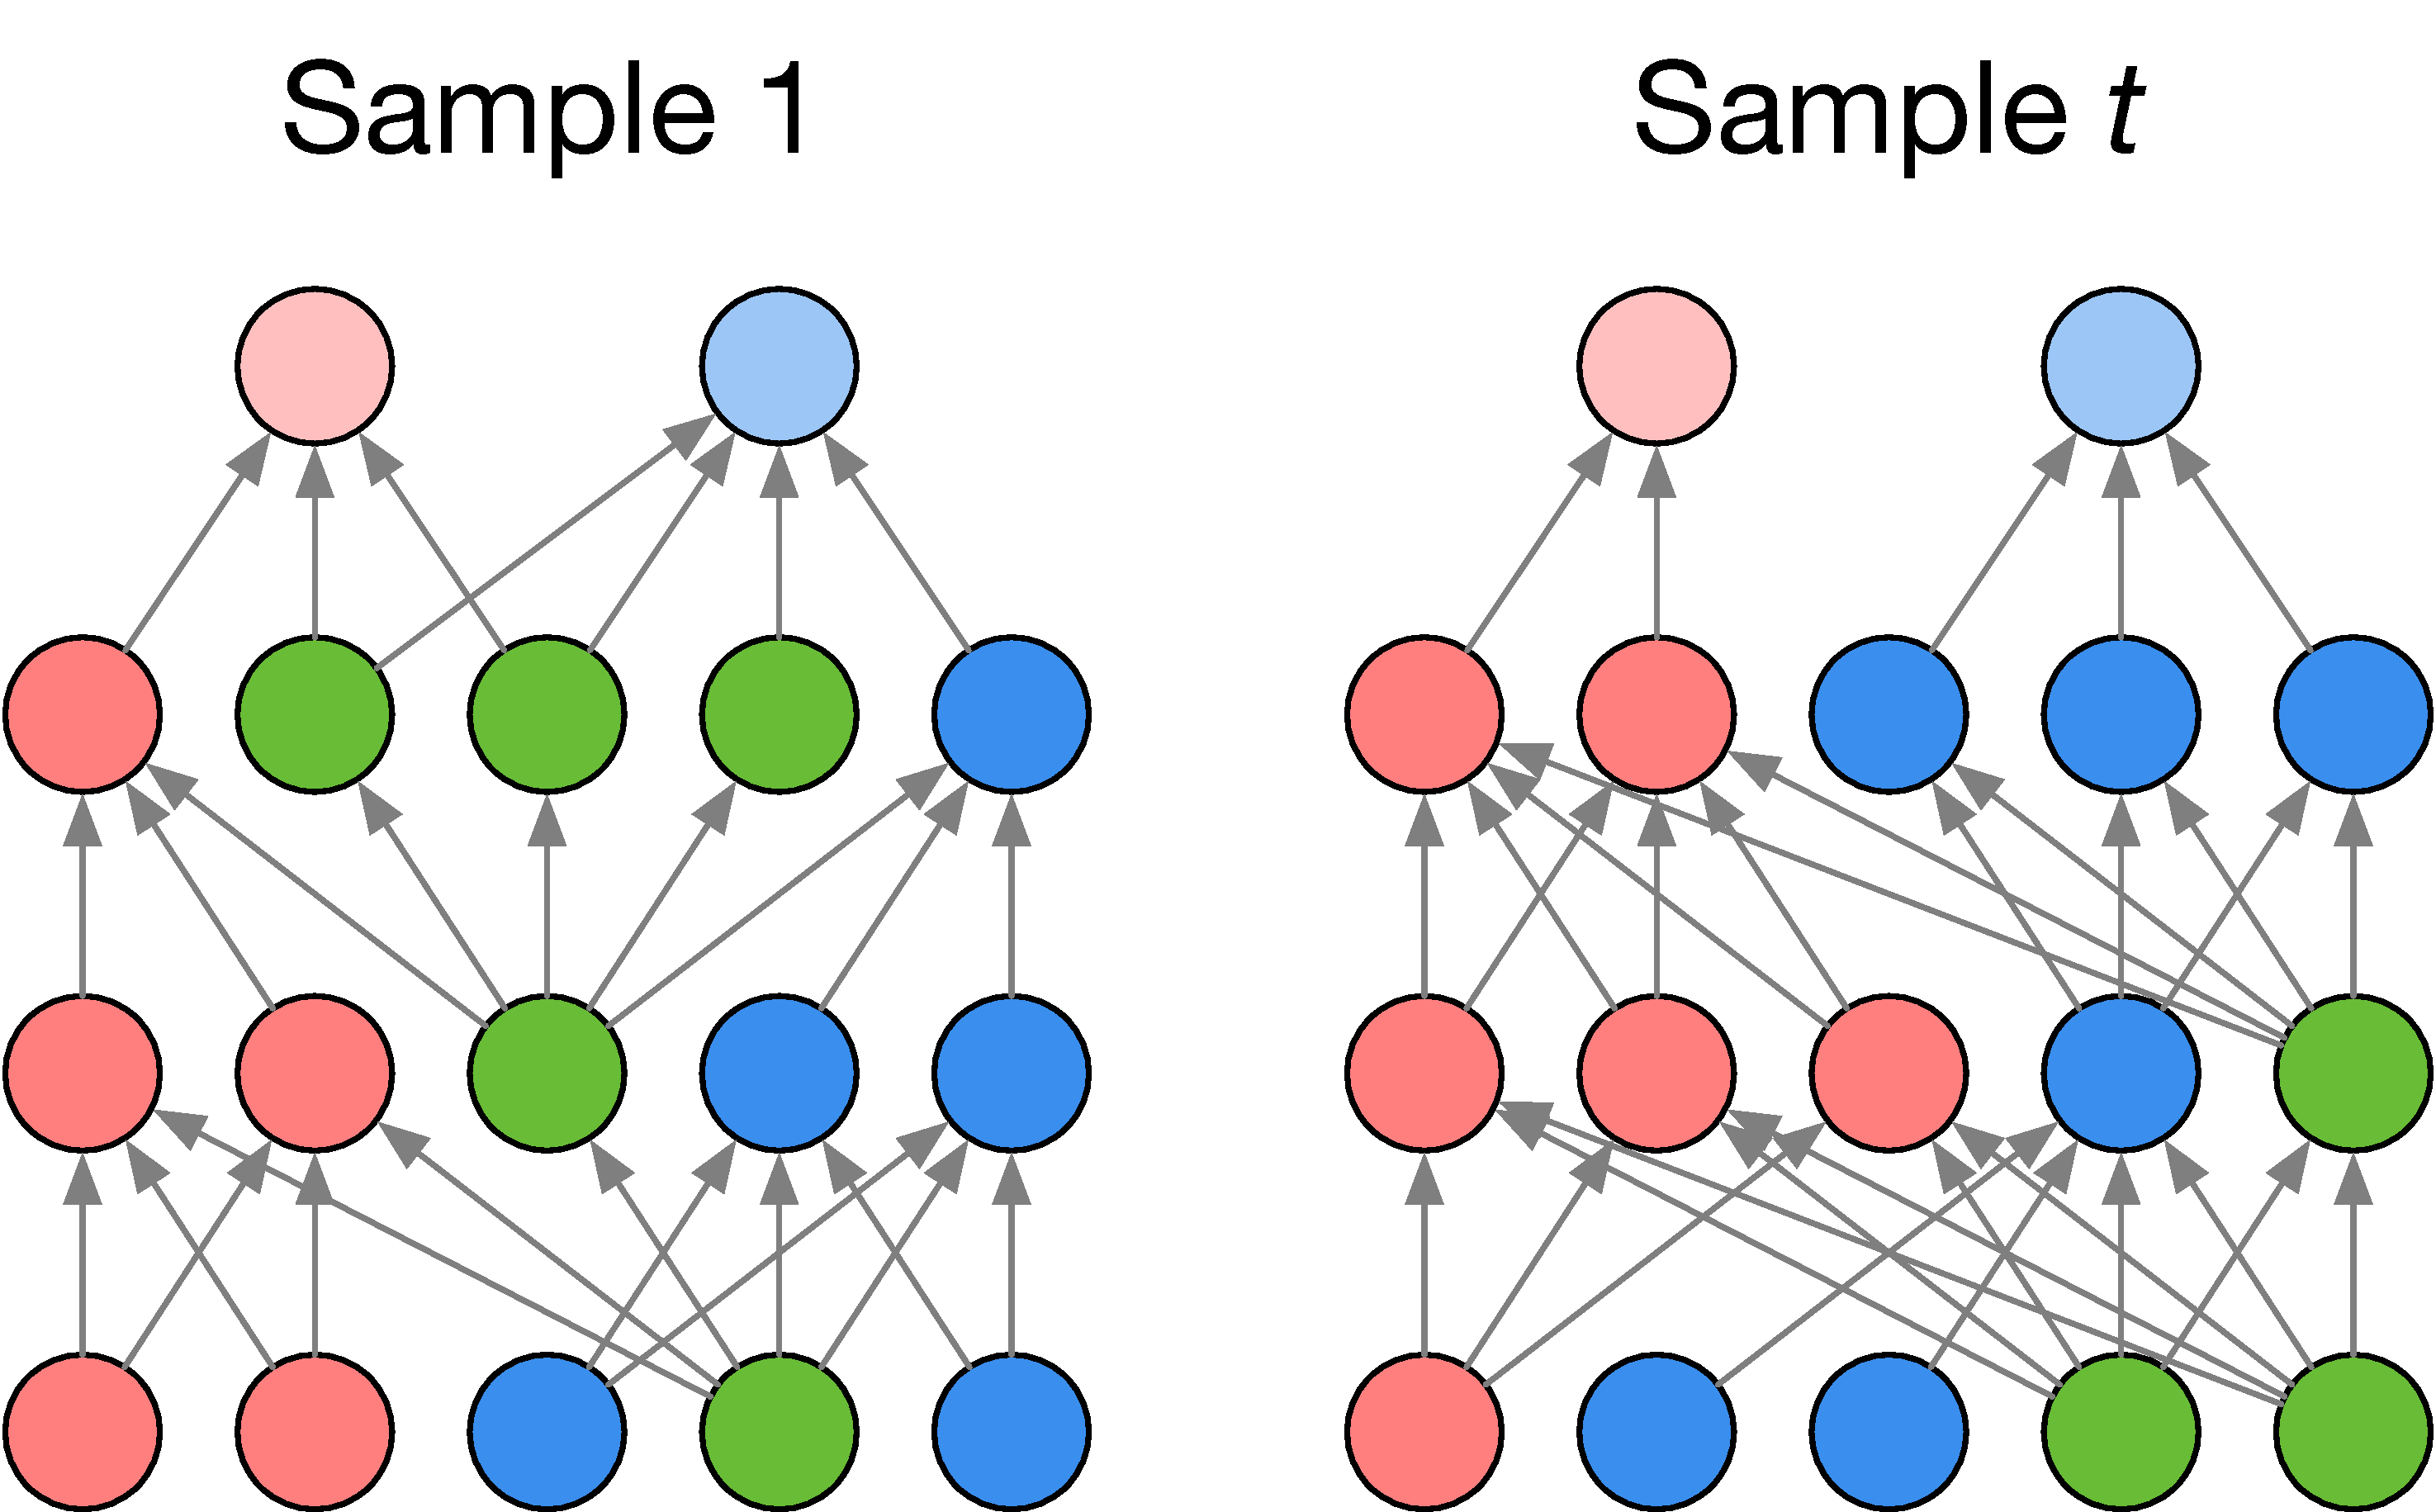
\includegraphics[width=0.8\linewidth]{chapter_6/figures/training_sampling.pdf}
% 	\caption{Illustration of sampling during training. Each circle denotes a set of activations from each filter group. Each arrow indicates }
%     \label{fig:sampling}
% \end{figure}



%%%%%%%%%%%%%%%%%%%%%%% RESULTS %%%%%%%%%%%%%%%%%%%%%%%%%%%%%%
\section{Experiments}\label{sec:experiments}
We tested \emph{stochastic filter groups} (SFG) on two multi-task learning (MTL) problems: 1) age regression and gender classification from face images on UTKFace dataset \cite{zhifei2017cvpr} and 2) semantic image regression (synthesis) and segmentation on a medical imaging dataset. 

    \paragraph{UTKFace dataset:} We tested our method on UTKFace \cite{zhifei2017cvpr}, which consists of 23,703 cropped faced images in the wild with labels for age and gender. We created a dataset with a 70/15/15\% split. We created a secondary separate dataset containing only 10\% of images from the initial set, so as to simulate a data-starved scenario.
    \paragraph{Medical imaging dataset:} We used a medical imaging dataset to evaluate our method in a real-world, multi-task problem where paucity of data is common and hard to mitigate. The goal of radiotherapy treatment planning is to maximise radiation dose to the tumour whilst minimising dose to the organs. To plan dose delivery, a Computed Tomography (CT) scan is needed as CT voxel intensity scales with tissue density, thus allowing dose propagation simulations. An MRI scan is needed to segment the surrounding organs. Instead of acquiring both an MRI and a CT, algorithms can be used to synthesise a CT scan (task 1) and segment organs (task 2) given a single input MRI scan. For this experiment, we acquired $15$ 3D prostate cancer scans with respective CT and MRI scans with semantic 3D labels for organs (prostate, bladder, rectum and left/right femur heads) obtained from a trained radiologist. We created a training set of $10$ patients, with the remaining $5$ used for testing. We trained our networks on 2D subimages of size $128$x$128$ randomly sampled from axial slices, and reconstructed the 3D volumes of size $288$x$288$x$62$ at test time by stitching together the subimage-wise predictions.

\subsection{Baselines}
We compared our model against four baselines in addition to Cross-Stitch networks \cite{MisraCrossMTL16} trained end-to-end rather than sequentially for fair comparison. The four baselines considered are: 1) single-task networks, 2) hard-parameter sharing multi-task network (MT-hard sharing), 3) SFG-networks with constant $\nicefrac{1}{3}$ allocated grouping (MT-constant mask) as \textit{per} Fig.~\ref{fig:different_grouping}(i), and 4) SFG-networks with constant grouping probabilities (MT-constant \textbf{p}). We train all the baselines in an end-to-end fashion for all the experiments. 

We note that all four baselines can be considered special cases of an SFG-network. Two \emph{single-task networks} can be learned when the shared grouping probability of kernels is set to zero. Considering Fig.~\ref{fig:schematic}, this would remove the diagonal connections and the shared network. This may be important when faced with two unrelated tasks which share no contextual information. A \emph{hard-parameter sharing network} exists when all shared grouping probabilities are maximised to one leading to a scenario where all features are shared within the network up until the task-specific layers. The \emph{MT-constant mask network} is illustrated in Fig.~ \ref{fig:different_grouping}(i), where $\nicefrac{1}{3}$ of kernels are allocated to the task $1$, task $2$ and shared groups, yielding uniform splits across layers. This occurs when an equal number of kernels in each layer obtain probabilities of $\mathbf{p}^{(l),k}=[1, 0, 0], [0, 1, 0]$ and $[0, 0, 1]$. Lastly, the \emph{MT-constant \textbf{p}} model represents the situation where the grouping is non-informative and each kernel has equal probability of being specific or shared with probability $\mathbf{p}^{(l),k}=[\nicefrac{1}{3}, \nicefrac{1}{3}, \nicefrac{1}{3}]$. \textcolor{black}{Training details for these models, including the hyper-parameter settings, are provided in the supplementary document.}

    \paragraph{UTKFace network:} We used VGG-11 CNN architecture \cite{vgg} for age and gender prediction. The network consists of a series of $3$x$3$ convolutional layers interleaved with max pooling layers. In contrast to the original architecture, we replaced the final max pooling and fully connected layers with global average pooling (GAP) followed by a fully connected layers for prediction. Our model's version of VGG (SFG-VGG) replaces each convolutional layer in VGG-11 with a SFG layer with max pooling applied to each feature map $F^{(l)}_{1}$, $F^{(l)}_{2}$, $F^{(l)}_{s}$. We applied GAP to each final feature map before the final merging operation and two fully connected layers for each task.
    
    \paragraph{Medical imaging network:} We used a high-resolution network architecture (HighResNet) \cite{wenqi} for CT synthesis and organ segmentation. This network has been successfully developed for semantic segmentation in medical imaging and has been used in a variety of medical applications such as CT synthesis \cite{bragman2018multi, kerstin}, brain segmentation \cite{wenqi} and tumour segmentation \cite{zach}. It consists of a series of residual blocks, which group two $3$x$3$ convolutional layers with dilated convolutions. The baseline network is composed of a $3$x$3$ convolutional layer followed by three sets of twice repeated residual blocks with dilated convolutions using factors $d=[1, 2, 4]$. There is a $3$x$3$ convolutional layer between each set of repeated residual blocks. The network ends with two final $3$x$3$ layers and either one or two $1$x$1$ convolutional layers for single and multi-task predictions. In our model, we replace each convolutional layer with an SFG module. After the first SFG layer, three distinct repeated residual blocks are applied to $F^{(l=0)}_{1}$, $F^{(l=0)}_{2}$, $F^{(l=0)}_{s}$. These are then merged according the feature routing methodology followed by a new SFG-layer and subsequent residual layers. Our model concludes with 2 successive SFG-layers followed by $1$x$1$ convolutional layers applied to the merged features $F^{(l=L)}_{1}$ and $F^{(l=L)}_{2}$. 

\begin{table}[h]
    \begin{subtable}[t]{0.49\linewidth}
    \footnotesize
    \caption{Full training data}
    \vspace{-5mm}
    \begin{center}
        \begin{tabular}{lccc}
        \hline
            \toprule
            \multirow{2}{*}{Method}                      & Age   & Gender     \\
                                                        & (MAE)   & (Accuracy)    \\
            \midrule
            One-task (VGG11) \cite{vgg}                       & $7.32$  & $90.70$                 \\
            \multirow{1}{*}{MT-hard sharing}   & $7.92$  & $90.60$ \\ 
            \multirow{1}{*}{MT-constant mask}   & $7.67$  & $89.41$                 \\
            \multirow{1}{*}{MT-constant \textbf{p}=[$\nicefrac{1}{3}$,$\nicefrac{1}{3}$,$\nicefrac{1}{3}$]}   & \cellcolor{blue!15} $6.34$  & \cellcolor{blue!15} $92.10$                 \\
            \multirow{1}{*}{VGG11 Cross Stitch \cite{MisraCrossMTL16}}   & $6.78$  & $90.30$                 \\
            \multirow{1}{*}{MT-SFG (ours)}       &  \cellcolor{red!15} $\mathbf{6.00}$  &  \cellcolor{red!15} $\mathbf{92.46}$                 \\
        \hline
        \end{tabular}
    \end{center}
    \label{tab:big_data}
    \end{subtable}
    \begin{subtable}[t]{0.49\linewidth}
    \footnotesize
    \caption{Small training data}
    \vspace{-5mm}
    \begin{center}
        \begin{tabular}{lccc}
        \hline
            \toprule
            \multirow{2}{*}{Method} & Age   & Gender     \\
            & (MAE)   & (Accuracy)    \\
            \midrule
            One-task (VGG11) \cite{vgg}                       & \cellcolor{blue!15}  $8.79$  & $85.54$                 \\
            \multirow{1}{*}{MT-hard sharing}   & $9.19$  & $85.83$                 \\
            \multirow{1}{*}{MT-constant mask}   & $9.02$  & $85.98$                \\
            \multirow{1}{*}{MT-constant \textbf{p}=[$\nicefrac{1}{3}$,$\nicefrac{1}{3}$,$\nicefrac{1}{3}$]}   & $9.15$  & \cellcolor{blue!15} $86.01$                 \\
            \multirow{1}{*}{VGG11 Cross Stitch \cite{MisraCrossMTL16}}   & $8.85$  &   $83.72$                 \\
            
            \multirow{1}{*}{MT-SFG (ours)}       & \cellcolor{red!15}  $\mathbf{8.54}$  &\cellcolor{red!15}  $\mathbf{87.01}$                 \\
    \hline
    \end{tabular}
    \end{center}
    \label{tab:small_data}
    \end{subtable}
\vspace{-3mm}
\caption{\small Age regression and gender classification results on UTKFace \cite{zhifei2017cvpr} with (a) the full and (b) limited training set. The best and the second best results are shown in red and blue. The mean absolute error (MAE) is reported for the age prediction and classification accuracy for gender prediction. For our model, we performed $50$ stochastic forward passes at test time by sampling the kernels from the approximate posterior $q_{\phi}(\mathcal{W})$. We calculated the average age per subject and obtained gender prediction using the mode of the test-time predictions. We initialised our model with grouping probabilities \textbf{p}=[0.2, 0.6, 0.2] for all convolution kernels.}

%\caption{Age regression and gender classification on the UTKFace \cite{zhifei2017cvpr} dataset in low training data regime; training on 1,770 subjects and validating on 18,374. We report the Mean Absolute Error for age regression and classification accuracy for gender prediction. AAAAA. Age regression and gender classification on the UTKFace \cite{zhifei2017cvpr} dataset on $3,550$ subjects. The multi-mask models can be visualised in Figure X. Results for our method were acquired after hyper-parameter optimisation (Gumbel-Softmax anneal rate and entropy weighting) on a different randomly generated training set. Inference iteration for the testing set was determined by analysis of the performance metrics on the validation set for each model.}
\label{tab:face_set}
\end{table}



%\caption{Results on 5-layer VGG with half the number of kernels per layer. MT-VGG 1 is a multi-task architecture with hard-parameter sharing with VGG as the representation network. MT-VGG 2 and MT-VGG 3 correspond to networks (a) and (b) in Figure X. We report multiple results for our method: a) using constant $\tau=0.5$ temperature for the Gumbel-Softmax and an annealing rate determined by max$(0.05,\text{exp}(-rt))$ where $r$ is a hyper-parameter determined on the validation set and $t$ corresponds to current iteration number in training. Inference iteration for the testing set was determined by analysis of performance metrics on the validation set for each model.}
%\end{table}

\section{Results}

\subsection{Age regression and gender prediction}

Results on age prediction and gender classification on both datasets are presented in Tab.~ \ref{tab:big_data} and \ref{tab:small_data}. Our model (MT-SFG) achieved the best performance in comparison to the baselines in both data regimes. In both sets of experiments, our model outperformed the hard-parameter sharing (\emph{MT-hard sharing}) and constant allocation (\emph{MT-constant mask}). This demonstrates the advantage of learning to allocate kernels. In the \emph{MT-constant mask} model, kernels are equally allocated across groups. In contrast, our model is able to allocate kernels in varying proportions across different layers in the network (Fig.~ \ref{fig:LEARNED_A} - SFG-VGG11) to maximise inductive transfer. Moreover, our methods performed better than a model with constant, non-informative grouping probabilities (\emph{MT-constant} \textbf{p}$= [\nicefrac{1}{3}, \nicefrac{1}{3}, \nicefrac{1}{3}]$), displaying the importance of learning structured representations and connectivity across layers to yield good predictions.

% hs - each task uses fewer number of parameters and we perform better

\begin{table*}[t!]
    \begin{subtable}[t]{1.0\linewidth}
        \caption{CT Synthesis (PSNR)}
        \vspace{-5mm}
        \begin{center}
            \scriptsize
            \begin{tabular}{l|c|ccccc}
            \hline
                \toprule
                Method   & Overall   &  Bones  & Organs &  Prostate & Bladder & Rectum  \\
                \midrule
                 One-task (HighResNet) \cite{wenqi} & $\,\,$ 25.76 (0.80)$\,\,$ & $\,\,$ 30.35 (0.58) $\,\,$  & $\,\,$ 38.04 (0.94) $\,\,$ & $\,\,$ 51.38 (0.79) $\,\,$ & $\,\,$ 33.34 (0.83)$\,\,$ & $\,\,$ 34.19 (0.31)$\,\,$  \\
                \multirow{1}{*}{MT-hard sharing }  & 26.31 (0.76) & 31.25 (0.61) & 39.19 (0.98) & 52.93 (0.95)  & 34.12 (0.82) & 34.15 (0.30) \\
                \multirow{1}{*}{MT-constant mask}   &  $24.43 (0.57)$  & $29.10 (0.46)$  & $37.24 (0.86)$ & $50.48 (0.73) $  & $32.29 (1.01)$ & $33.44 (2.88)$  \\
                \multirow{1}{*}{MT-constant \textbf{p}=[$\nicefrac{1}{3}$,$\nicefrac{1}{3}$,$\nicefrac{1}{3}$]}   & 26.64(0.54)  & 31.05 (0.55) & 39.11 (1.00)    & \cellcolor{blue!15} 53.20 (0.86)  & 34.34 (1.35) &  35.61 (0.35) \\
                \multirow{1}{*}{Cross Stitch \cite{MisraCrossMTL16}}   & \cellcolor{red!15}  27.86 (1.05)  & \cellcolor{blue!15}  32.27 (0.55)  & \cellcolor{red!15}  40.45 (1.27)  & \cellcolor{red!15} 54.51 (1.01)     & \cellcolor{red!15}  36.81 (0.92) &  \cellcolor{red!15} 36.35 (0.38)     \\
                \multirow{1}{*}{MT-SFG (ours)}  &   \cellcolor{blue!15} 27.74 (0.96) &  \cellcolor{red!15}  32.29 (0.59)&  \cellcolor{blue!15}  39.93 (1.09)& 53.01 (1.06)   &  \cellcolor{blue!15} 35.65 (0.44)& \cellcolor{blue!15} 35.65 (0.37)  \\
        \hline
        \end{tabular}
        \end{center}
    \label{tab:ct}
    \end{subtable}
    
    \begin{subtable}[t]{1.0\linewidth}
        \vspace{0mm}
        \caption{Segmentation (DICE)}
        \vspace{-5mm}
        \begin{center}
            \centering
            \scriptsize
            \begin{tabular}{l|c|ccccc}
            \hline
                \toprule
                Method & Overall  &   Left Femur Head &  Right Femur Head &  Prostate & Bladder & Rectum   \\
                
                \midrule
                One-task (HighResNet) \cite{wenqi} & $0.848 (0.024)$ & 0.931 (0.012)  & \cellcolor{blue!15} 0.917 (0.013)   & 0.913 (0.013) & 0.739 (0.060)  & 0.741 (0.011)  \\
                
                \multirow{1}{*}{MT-hard sharing }  & $0.829 (0.023)$ & \cellcolor{blue!15} 0.933 (0.009)  & 0.889 (0.044)    &  0.904 (0.016) & 0.685 (0.036)   &  0.732 (0.014) \\
               
                \multirow{1}{*}{MT-constant mask}  & $0.774 (0.065)$ & 0.908 (0.012)  & 0.911 (0.015)    &0.806 (0.0541)   & 0.583 (0.178)  & 0.662 (0.019) \\
                \multirow{1}{*}{MT-constant \textbf{p}=[$\nicefrac{1}{3}$,$\nicefrac{1}{3}$,$\nicefrac{1}{3}$]}   & $0.752 (0.056)$ &   0.917 (0.004)& \cellcolor{red!15} 0.917 (0.01)&0.729 (0.086)   & 0.560 (0.180)  &0.639 (0.012)\\
                 \multirow{1}{*}{Cross Stitch \cite{MisraCrossMTL16}}  &\cellcolor{red!15}  0.854 (0.036) & 0.923 (0.008)   &  0.915 (0.013) &   \cellcolor{red!15} 0.933 (0.009)  &  \cellcolor{red!15} 0.761 (0.053)   &   \cellcolor{blue!15} 0.737 (0.015)\\
                 \multirow{1}{*}{MT-SFG (ours)}  &  \cellcolor{blue!15}  $0.852 (0.047)$ &  \cellcolor{red!15} 0.935 (0.007)  & 0.912 (0.013)   &  \cellcolor{blue!15} 0.923 (0.016)  &  \cellcolor{blue!15}  0.750 (0.062) &  \cellcolor{red!15} 0.758 (0.011) \\
        \hline
        \end{tabular}
        \end{center}
    \label{tab:seg}
    \end{subtable}

\vspace{-3mm}
\caption{\small Performance on the medical imaging dataset with best results in red, and the second best results in blue. The PSNR is reported for the CT-synthesis (synCT) across the whole volume (overall), at the bone regions, across all organ labels and individually at the prostate, bladder and rectum. For the segmentation, the average DICE score per patient across all semantic labels is computed. The standard deviations are computed over the test subject cohort. For our model, we perform $50$ stochastic forward passes at test-time by sampling the kernels from the approximated posterior distribution $q_{\phi}(\mathcal{W})$. We compute the average of all passes to obtain the synCT and calculate the mode of the segmentation labels for the final segmentation. We initialised our model with grouping probabilities \textbf{p}=[0.2, 0.6, 0.2]. Red cells indicate best performing and blue cells indicate second best models.}
%\caption{Performance metrics for synthetic CT regression (synCT) and organ segmentation. We calculated the mean absolute error (MAE) for the regression and the average DICE score across segmented organs for the segmentation task (Seg). We report the mean ($\pm$ st.d.) across patients. Results for our method were acquired after hyper-parameter optimisation (Gumbel-Softmax anneal rate and entropy weighting) on a different randomly generated training set. Inference iteration for the testing set was determined after convergence of the training loss.}
\label{tab:medicalimaging}
\end{table*}


\subsection{Image regression and semantic segmentation}
Results on CT image synthesis and organ segmentation from input MRI scans is detailed in Tab.~\ref{tab:medicalimaging}. Our method obtains equivalent (non-statistically significant different) results to the Cross-Stitch network \cite{MisraCrossMTL16} on both tasks. We have, however, observed best synthesis performance in the bone regions (femur heads and pelvic bone region) in our model when compared against all the baselines, including Cross-Stitch. The bone voxel intensities are the most difficult to synthesise from an input MR scan as task uncertainty in the MR to CT mapping at the bone is often highest \cite{bragman2018multi}. Our model was able to disentangle features specific to the bone intensity mapping (Fig.~ \ref{fig:activations}) without supervision of the pelvic location, which allowed it to learn a more accurate mapping of an intrinsically difficult task. 


% \begin{subtable}[t]{0.9\linewidth}
%     \caption{CT Synthesis (PSNR)}
%     \vspace{-5mm}
%     \begin{center}
%         \footnotesize
%         \begin{tabular}{l|cccccc|c}
%         \hline
%             \toprule
%             \multirow{2}{*}{Method}  &  &   & synCT (PSNR)   &   &  & & Seg (DICE)   \\
%                             & Whole   &  Bones  & Organs &  Prostate & Bladder & Rectum &  Whole   \\
%             \midrule
%             One-task (HighResNet) \cite{wenqi} & 25.76 (0.80) & 30.35 (0.58)  & 38.04 (0.94) & 51.38 (0.79)& 33.34 (0.83) & 34.19 (0.31) & $0.8483 (0.0239)$  \\
%             \multirow{1}{*}{MT-hard sharing }  & 26.31 (0.76) & 31.25 (0.61) & 39.19 (0.98) & 52.93 (0.95)  & 34.12 (0.82) & 34.15 (0.30)& $0.8285 (0.0231)$ \\
%             \multirow{1}{*}{MT-constant mask}   & $24.43 (0.57)$  & $29.10 (0.46)$  & $37.24 (0.86)$ & $50.48 (0.73) $  & $32.29 (1.01)$ & $33.44 (2.88)$ & $0.7741 (0.0645)$  \\
%             \multirow{1}{*}{MT-constant \textbf{p}=[$\nicefrac{1}{3}$,$\nicefrac{1}{3}$,$\nicefrac{1}{3}$]}   & 26.64(0.54)  & 31.05 (0.55) & 39.11 (1.00)    & \cellcolor{blue!15} 53.20 (0.86)  & 34.34 (1.35) & \cellcolor{blue!15} 35.65 (3.50) & $0.7529 (0.0563)$\\
%             \multirow{1}{*}{Cross Stitch \cite{MisraCrossMTL16}}   & \cellcolor{red!15}  27.86 (1.05)  & \cellcolor{blue!15}  32.27 (0.55)  & \cellcolor{red!15}  40.45 (1.27)  & \cellcolor{red!15} 54.51 (1.01)     & \cellcolor{red!15}  36.81 (0.92) &  \cellcolor{red!15} 36.35 (3.83) &  \cellcolor{red!15} 0.8544 (0.0368)      \\
%             \multirow{1}{*}{MT-SFG (ours)}  &   \cellcolor{blue!15} 27.74 (0.96) &  \cellcolor{red!15}  32.29 (0.59)&  \cellcolor{blue!15}  39.93 (1.09)& 53.01 (1.06)   &  \cellcolor{blue!15} 35.65 (0.44)&  35.61 (0.37) &  \cellcolor{blue!15} $0.8517 (0.0269)$ \\
%     \hline
%     \end{tabular}
%     \end{center}
% \end{subtable}



%\begin{figure}[b!]
%	\center
%	\vspace{-3mm}
%	\includegraphics[width=1.2\linewidth]{chapter_6/figures/p_1.png}
%	\caption{Learned architecture in SFG-ResNet}
 %   \label{fig:performance_on_small_data}
%\end{figure}

% \begin{figure}[ht]
% 	\center
% 	\vspace{-3mm}
% 	\includegraphics[width=1\linewidth]{chapter_6/figures/p_2.png}
% 	\caption{Learned architecture in SFG-ResNet}
%     \label{fig:performance_on_small_data}
% \end{figure}

%\begin{figure}[ht]
%	\center
%	\vspace{-3mm}
%	\includegraphics[width=1.2\linewidth]{chapter_6/figures/f_1.png}
%	\caption{Learned architecture in SFG-VGG}
 %   \label{fig:sfg-vgg}
%\end{figure}

%\begin{figure}[ht]
%	\center
%	\vspace{-3mm}
%	\includegraphics[width=1\linewidth]{chapter_6/figures/f_2.png}
%	\caption{Learned architecture in SFG-VGG}
 %   \label{fig:performance_on_small_data}
%\end{figure}

%st - 7.64/85.963
%mt 8.18, 86.63


\subsection{Learned architectures} \label{sec:learned_architecture}

\begin{figure*}[ht]
	%\hspace{0.075\linewidth}
	\center
	\includegraphics[width=\linewidth]{chapter_6/figures/FINAL.pdf}
	\caption{\small Activation maps from example kernels in the learned task-specific and shared filter groups, $G^{(l)}_{1}, G^{(l)}_{2}, G^{(l)}_{s}$ (enclosed in blue, green and pink funnels) in the first, the second last and the last convolution layers in the SFG-HighResNet model trained on the medical imaging dataset. The results from convolution kernels with low entropy (i.e. high ``confidence'') of group assignment probabilities $\mathbf{p}^{(l)}$  are shown for the respective layers.  }
	\label{fig:activations}
\end{figure*}

Analysis of the grouping probabilities of a network embedded with SFG modules permits visualisation of the network connectivity and thus the learned MTL architecture. To analyse the group allocation of kernels at each layer, we computed the sum of class-wise probabilities per layer. Learned groupings for both SFG-VGG11 network trained on UTKFace and the SFG-HighResNet network trained on prostate scans are presented in Fig.~ \ref{fig:LEARNED_A}. These figures illustrate increasing task specialisation in the kernels with network depth. At the first layer, all kernels are classified as shared (\textbf{p}$=[0, 1, 0]$) as low-order features such as edge or contrast descriptors are generally learned earlier layers. In deeper layers, higher-order representations are learned, which describe various salient features specific to the tasks. This coincides with our network allocating kernels as task specific, as illustrated in Fig.~\ref{fig:activations}, where activations are stratified by allocated class per layer. \textcolor{black}{Density plots of the learned kernel probabilities and trajectory maps displaying training dynamics, along with more examples of feature visualisations, are provided in supplementary materials.}

Notably, the learned connectivity of both models shows striking similarities to hard-parameter sharing architectures commonly used in MTL. Generally, there is a set of shared layers, which aim to learn a feature set common to both tasks. Task-specific branches then learn a mapping from this feature space for task-specific predictions. Our models are able to automatically learn this structure whilst allowing asymmetric allocation of task-specific kernels with no priors on the network structure.

\begin{figure}[ht]
	\center
	\vspace{-3mm}
	\includegraphics[width=1.0\linewidth]{chapter_6/figures/learned_a.pdf}
	\caption{\small Learned kernel grouping in a) SFG-VGG11 network on UTKFace and b) SFG-HighResNet on medical scans. The proportions of task-1, shared and task-2 filter groups are shown in blue, green and pink. Within SFG-VGG11, task-1 age regression and task-2 is gender classification. For SFG-HighResNet, task-1 is CT synthesis and task-2 is organ segmentation. }
	\vspace{-3mm}
    \label{fig:LEARNED_A}
\end{figure}


\subsection{Effect of \textbf{p} initialisation}
Fig.~\ref{fig:different_grouping} shows the layer-wise proportion of the learned kernel groups on the UTKFace dataset for four different initilization schemes of grouping probabilities $\mathbf{p}$: (i) ``dominantly shared'', with $\mathbf{p}=[0.2, 0.6, 0.2]$, (ii) ``dominantly task-specific'', with $\mathbf{p}=[0.45, 0.1, 0.45]$, (iii) ``random'', where $\mathbf{p}$ is drawn from $\text{Dirichlet}(1,1,1)$, (iv) ``start with MT-constant mask", where an equal number of kernels in each layer are set to probabilities of $\mathbf{p}= [1,0,0],[0,1,0]$ and $[0,0,1]$. In all cases, the same set of hyper-parameters, including the annealing rate of the temperature term in GSM approximation and the coefficient of the entropy regularizer $\mathcal{H}(\mathbf{p})$, were used during training. We observe that the kernel grouping of respective layers in (i), (ii) and (iii) all converge to a very similar configuration observed in Sec.~\ref{sec:learned_architecture}, highlighting the robustness of our method to different initialisations of $\mathbf{p}$. In case (iv), the learning of $p$ were much slower than the remaining cases, due to weaker gradients, and we speculate that a higher entropy regularizer is necessary to facilitate its convergence. 


\begin{figure}[ht]
	\center
	\includegraphics[width= \linewidth]{chapter_6/figures/DIFFERENT_P.pdf}
	\caption{Effect of the initial values of grouping probabilities $\mathbf{p}$ on the learned kernel allocation after convergence. }
    \label{fig:performance_on_small_data}
\end{figure}



%%%%%%%%%%%%%%%%%%%%%%% Discussion %%%%%%%%%%%%%%%%%%%%%%%%%%%%%%
\section{Discussion}

In this paper, we have proposed \emph{stochastic filter groups} (SFGs) to disentangle \emph{task-specific} and \emph{generalist} features. SFGs probabilistically defines the grouping of kernels and thus the connectivity of features in a CNNs. We use variational inference to approximate the distribution over connectivity given training data and sample over possible architectures during training. Our method can be considered as a probabilistic form of multi-task architecture learning \cite{liang2018evolutionary}, as the learned posterior embodies the optimal MTL architecture given the data.

Our model learns structure in the representations. The learned shared (generalist) features may be exploited either in a transfer learning or continual learning scenario. As seen in \cite{lacost2018}, an effective prior learned from multiple tasks can be a powerful tool for learning new, unrelated tasks. Our model consequently offers the possibility to exploit the learned task-specific and generalist features when faced with situations where a third task is needed, which may suffer from unbalanced or limited training data. This is particularly relevant in the medical field, where training data is expensive to acquire as well as laborious. We will investigate this in further work.

Lastly, a network composed of SFG modules can be seen as a superset of numerous MTL architectures. Depending on the data and the analysed problem, SFGs can recover many different architectures such as single task networks, traditional hard-parameter sharing, equivalent allocation across tasks, and asymmetrical grouping (Fig.~\ref{fig:different_grouping}). Note, however, that proposed SFG module only learns connectivity between neighbouring layers. Non-parallel ordering of layers, a crucial concept of MTL models \cite{meyerson2018beyond, Ruder2019SluiceNL}, was not investigated. Future work will look to investigate the applicability of SFG modules for learning connections across grouped kernels between non-neighbouring layers.


%Discuss some limitations and future outlook, too. In this work, we do not explicitly enforce task-invariance or task-specificity, and this could potentially lead to "leakage" of features whereby some task-specific features are learned as a part of the shared features and the vice versa. 

% \subsection{Limitations of cross-sftitch module}
% \begin{enumerate}
%     \item Does not guarantee task-specific features
%     \item No end to end training
%     \item Learned parameters for sharing are useless in the context of exploiting sharing for new tasks
% \end{enumerate}



%%%%%%%%%%%%%%%%%%%%%%%%%%%%%%%%%%%%%%%%%
%%%%%%%%%%%% SUPPLEMENTARY MATERIALS %%%%%%%%%%%%%%
%%%%%%%%%%%%%%%%%%%%%%%%%%%%%%%%%%%%%%%%%
%
%\section{Training and implementation details}
%\subsection{Optimisation, regularisation and initialisation}
%All networks were trained with ADAM optimiser \cite{ADAM} with an initial learning rate of $10^{-3}$ and $\beta = [0.9, 0.999]$. We used values of $\lambda_1=10^{-6}$ and $\lambda_2=10^{-5}$ for the weight and entropy regularisation factors in Equation $(5)$ in Section $3.2$. All \emph{stochastic filter group} (SFG) modules were initialised with grouping probabilities \textbf{p}=[$0.2$, $0.6$, $0.2$] for every convolution kernel. Positivity of the grouping probabilities $\textbf{p}$ is enforced by passing the output through a \emph{softplus} function $f(x)=\text{ln}(1+e^{x})$ as in \cite{lakshminarayanan2017simple}. The scheduler $\tau = \text{max}(0.10, \exp(-rt))$ recommended in \cite{jang2016categorical} was used to anneal the Gumbel-Softmax temperature $\tau$ where $r$ is the annealing rate and $t$ is the current training iteration. We used $r=10^{-5}$ for our models.
%
%Hyper-parameters for the annealing rate and the entropy regularisation weight were obtained by analysis of the network performance on a secondary randomly split on the UTK dataset ($70/15/15$). They were then applied to all trained models (large and small dataset for UTKFace and medical imaging dataset).
%
%\subsection{UTKFace}
%For training the VGG networks (Section 4.1 - UTKFace network), we used the root-mean-squared-error (RMSE) for age regression and the cross entropy loss for gender classification. The labels for age were divided by $100$ prior to training. The input RGB images ($200$x$200$x$3$) were all normalised channel wise to have unit variance and zero mean prior to training and testing. A batch-size of $10$ was used. No augmentation was applied. We monitored performance during training using the validation set ($n=3554$) and trained up to $330$ epochs. We performed $150$ validation iterations every $1000$ iterations, leading to $1500$ predictions per validation iteration. Performance on the validation set was analysed and the iteration where Mean Absolute Error (MAE) was minimised and classification Accuracy was maximised was chosen for the test set.
%
%\subsection{Medical imaging dataset}
%We used T2-weighted Magnetic Resonance Imaging (MRI) scans (3T, 2D spin echo, TE/TR: 80/2500ms, voxel size 1.46x1.46x5mm$^{3}$) and Computed Tomography (CT) scans (140 kVp, voxel size 0.98x0.98x1.5 mm$^{3}$). The MR and CT scans were resampled to isotropic resolution (1.46mm$^{3}$). We performed intensity non-uniformity correction on the MR scans \cite{Tustison2010}.
%
%In the HighResNet networks (Section 4.1 - Medical imaging network), we used the RMSE loss for the regression task and the Dice + Cross-Entropy loss \cite{dicex} for the segmentation task. The CT scans were normalised using the transformation $\nicefrac{\text{CT}}{1024} + 1$. The original range of the CT voxel intensity was $[-1024,2500]$ with the background set to $-1024$. The input MRI scans were first normalised using histogram normalisation based on the $1^{st}$ and $99^{th}$ percentile \cite{Nyul2000}. The MRI scans were then normalised to zero mean and unit variance. At test time, input MRI scans were normalised using the histogram normalisation transformation obtained from the training set then normalised to have zero mean and unit variance. 
%
%All scans were of size $288$x$288$x$62$. We sub-sampled random patches from random axial slices of size $128$x$128$. We sampled from all axial slices in the volume ($n=62$). We trained up to $200,000$ iterations using a batch-size of $10$. We applied augmentation to the randomly sampled patches using random scaling factors in the range $[-10\%, 10\%]$ and random rotation angles in the range [$-10^\circ$, $10^\circ$]. The trained patches were zero-padded to increase their size to $136$x$136$. However, the loss during training was only calculated in non-padded regions.
%
%The inference iteration for the test set was determined when the performance metrics on the training set (Mean Absolute Error and Accuracy) first started to converge for at least $10,000$ iterations. In our model where the grouping probabilities were learned, the iteration when convergence in the update of the grouping probabilities was first observed was selected since performance generally increased as the grouping probabilities were updated. 
%
%\subsection{Implementation details}
%We used Tensorflow and implemented our models within the NiftyNet framework \cite{Gibson2018}. Models were trained on NVIDIA Titan Xp, P6000 and V100. All networks were trained in the Stochastic Filter Group paradigm. Single-task networks were trained by hard-coding the allocation of kernels to task $1$ and task $2$ i.e. $50$\% of kernels per layer were allocated to task $1$ and $50$\% were allocated to task $2$ with constant probabilities \textbf{p}=[1,0,0] and \textbf{p}=[0,0,1] respectively. The multi-task hard parameter sharing (MT hard-sharing) network was trained by hard-coding the allocation of kernels to the shared group i.e. $100$\% of kernel per layer were allocated to the shared group with constant probability \textbf{p}=[0, 1, 0]. The cross-stitch (CS) \cite{MisraCrossMTL16} networks were implemented in a similar fashion to the single-task networks, with CS modules applied to the output of the task-specific convolutional layers. The other baselines (MT-constant mask and MT-constant \textbf{p}=[\nicefrac{1}{3}, \nicefrac{1}{3}, \nicefrac{1}{3}]) were trained similarly.
%
%We used Batch-Normalisation \cite{ioffe2015batch} to help stabilise training. We observed that the deviation between population statistics and batch statistics can be high, and thus we did not use population statistic at test time. Rather, we normalised using batch-statistics instead, and this consistently lead to better predictive performance. We also used the Gumbel-Softmax approximation \cite{jang2016categorical} at test-time using the temperature value $\tau$ that corresponded to the iteration in $\tau$ annealing schedule.
%
%\section{CNN architectures and details}
%We include schematics and details of the single-task VGG11 \cite{vgg} and HighResNet \cite{wenqi} networks in Fig.~\ref{fig:supp_baselines}. In this work, we constructed multi-task architectures by augmenting these networks with the proposed SFG modules. We used the PReLU activation function \cite{prelu} in all networks. For the residual blocks used in the HighResNet networks in Fig.~\ref{fig:supp_baselines} (ii), we applied PReLU and batch-norm as pre-activation \cite{preactivation} to the convolutional layers. The SFG module was used to cluster the kernels in every coloured layer in Fig.~\ref{fig:supp_baselines}, and distinct sets of additional transformations (pooling operations for VGG and high-res blocks for HighResNet) were applied to the outputs of the respective filter groups $G_{1}, G_{2}, G_{s}$. For a fair comparison, the CS units \cite{MisraCrossMTL16} were added to the same set of layers.
%
%For clarification, the SFG layer number $n$ (e.g. SFG layer 2) corresponds to the $n^{th}$ layer with an SFG module. In the case of SFG-VGG11, each convolutional layer uses SFGs. The SFG layer number thus corresponds with layer number in the network. In the case of SFG-HighResNet, not every convolutional layer uses SFGs such as those within residual blocks. Consequently, SFG layer 1 corresponds to layer 1, SFG layer 2 is layer 6, SFG layer 3 is layer 11, SFG layer 4 is layer 16 and SFG layer 5 is layer 17.
%
%\begin{figure*}[h]
%    \centering
%    \includegraphics[width=0.80\textwidth]{chapter_6/figures_supp/supp_single_task.pdf}
%    \caption{Illustration of the single-task architectures, (i) VGG11 and (ii) HighResNet used for UTKFace and medical imaging dataset, respectively. In each architecture, the coloured components indicate the layers to which SFG or cross-stitch (CS) modules are applied when extended to the multi-task learning scenario, whilst the components in black denote the additional transformations applied to the outputs of respective filter groups or CS operations (see the description of black circles in the schematic provided in Fig.~5 of the main text)}. 
%    \label{fig:supp_baselines}
%\end{figure*}
%
%
%\section{Learned grouping probability plots}
%In this section, we illustrate density plots of the learned grouping probabilities $\mathbf{p}$ for each trained network (Fig.~\ref{fig:fig_learned_A} and Fig.~\ref{fig:fig_learned_B}). We also plot the training trajectories of grouping probabilities $\mathbf{p}$ of all kernels in each layer. These are colour coded by iteration number---blue for low and yellow for high iteration number. This shows that some grouping probabilities are quickly learned in comparison to others. 
%
%Fig.~\ref{fig:fig_learned_A} and Fig.~\ref{fig:fig_learned_B} show that most kernels are in the shared group at earlier layers of the network where mostly low-order generic features are learned (as illustrated in Fig.~ \ref{fig:act}, SFG layer $1$). They converge quickly to the shared vertex of the $2$-simplex as evidenced by the colour of the trajectory plots. As the network depth increases, task-specialisation in the kernels increases (see Fig.~ \ref{fig:act}, SFG layer $\ge4$). This is illustrated by high density clusters at task-specific vertices and by the trajectory plots.
%
%\begin{figure*}[ht!]
%    \vspace{-2mm}
%    \centering
%    \includegraphics[width=0.9\textwidth]{chapter_6/figures_supp/face_learning.pdf}
%    \caption{Density plots and trajectory plots of the learned grouping probabilities for the SFG-VGG11 architecture. The density plots represents the final learned probabilities per layer for each kernel. The trajectory plots represent how the grouping probabilities are learned during training and thus how the connectivity is determined. Histograms of the grouping probabilities were smoothed with a Gaussian kernel with $\sigma=1$. The densities are mapped to and visualised in the $2$-simplex using \texttt{python-ternary} \cite{ternary}.}
%    \label{fig:fig_learned_A}
%\end{figure*}
%
%
%\begin{figure*}[ht]
%    \centering
%    \vspace{-5mm}
%    \includegraphics[width=1.0\textwidth]{chapter_6/figures_supp/prostate_learning.pdf}
%    \caption{Density plots and trajectory plots of the learned grouping probabilities for the SFG-HighResNet architecture. The density plots represents the final learned probabilities per layer for each kernel. The trajectory plots represent how the grouping probabilities are learned during training and thus how the connectivity is determined.}
%    \label{fig:fig_learned_B}
%    \vspace{-5mm}
%\end{figure*}
%
%
%\section{Extra visualisation of activations}
%Here we visualise the activation maps of additional specialist and generalist kernels on the medical imaging dataset. To classify each kernel according to the group (task 1, task 2 or shared), we selected the group with the respective maximum assignment probability. The corresponding activation maps for various input images in the medical imaging dataset can be viewed in Fig.~\ref{fig:act} and Fig.~\ref{fig:act_unc}. 
%
%We first analysed the activation maps generated by kernels with low entropy of $\mathbf{p}$ (i.e. highly confident group assignment). At the first layer, all kernels are classified as shared, and the examples in Fig.~\ref{fig:act} support that these kernels tend to account for low-order features such as edge and contrast of the images. On the other hand, at deeper layers, higher-order representations are learned, which describe various salient features specific to the tasks such as organs for segmentation, and bones for CT-synthesis. Note that the bones are generally the most difficult region to synthesise CT intensities from an input MR scan \cite{bragman2018multi}.
%
%Secondly, we looked at activation maps from kernels with high entropy of $\mathbf{p}$ (i.e. highly uncertain group assignment) in Fig.~\ref{fig:act_unc}. In contrast to Fig.~\ref{fig:act}, the learned features do not appear to capture any meaningful structures for both synthesis and segmentation tasks. Of particular note is the dead kernel in the top row of the figure; displaying that a high uncertainty in group allocation correlates with non-informative features. 
%
%\begin{figure*}[h]
%    \centering
%    \vspace{-4mm}
%    \includegraphics[width=0.8\textwidth]{chapter_6/figures_supp/figure_1.pdf}
%    \vspace{-2mm}
%    \caption{Example activations for kernels with low entropy of $\mathbf{p}$ (i.e. group assignment with high confidence) for three input MR slices in the SFG-HighResNet multi-task network. Columns ``Shared'', ``Task 1'' \& ``Task 2'' display the results from the shared, CT-synthesis and organ-segmentation specific filter groups in respective layers. We illustrate activations stratified by group in layer $1$ (SFG layer 1), layer $16$ (SFG layer 4) and layer $17$ (SFG layer 5). }
%    \label{fig:act}
%    \vspace{-1mm}
%\end{figure*}
%
%\begin{figure*}[h]
%    \centering
%    \includegraphics[width=0.85\textwidth]{chapter_6/figures_supp/uncertain_activation.pdf}
%    \caption{Example activations for kernels with high entropy (i.e. group assignment with low confidence) for three input MR slices in the SFG-HighResNet multi-task network.  Columns ``Shared'', ``Task 1'' \& ``Task 2'' display the results from the shared, CT-synthesis and organ-segmentation specific filter groups in respective layers. We illustrate activations stratified by group in layer $16$ (SFG layer 4) and layer $17$ (SFG layer 5). }
%    \label{fig:act_unc}
%\end{figure*}
%
%
%\section{Learned filter groups on duplicate tasks}
%We analysed the dynamics of a network with SFG modules when trained with two duplicates of the same CT regression task (instead of two distinct tasks). Fig.~\ref{fig:duplicate} visualises the learned grouping and trajectories of the grouping probabilities during training. In the first $3$ SFG layers (layers $1$, $6$ and $11$ of the network), all the kernels are grouped as shared. In the penultimate SFG layer (layer $16$), either kernels are grouped as shared or with probability \textbf{p}=[\nicefrac{1}{2}, 0, \nicefrac{1}{2}], signifying that the kernels can belong to either task. The final SFG layer (layer $17$) shows that most kernels have probabilities \textbf{p}=[\nicefrac{1}{3}, \nicefrac{1}{3}, \nicefrac{1}{3}]. Kernels thus have equal probability of being task-specific or shared. This is expected as we are training on duplicate tasks and therefore the kernels are equally likely to be useful across all groups.
%
%\begin{figure*}[h]
%    \centering
%    \includegraphics[width=1.0\textwidth]{chapter_6/figures_supp/final_dup.pdf}
%    \caption{Top: density plots for the learned grouping probabilities at each SFG layer in a model where we trained on duplicate tasks i.e. task 1 is CT synthesis and task 2 is also CT synthesis. Bottom: trajectories of the grouping probabilities during training.}
%    \label{fig:duplicate}
%\end{figure*}

% %%%%%%%% ICML 2019 EXAMPLE LATEX SUBMISSION FILE %%%%%%%%%%%%%%%%%
%\documentclass{article}
%% Recommended, but optional, packages for figures and better typesetting:
%\usepackage{microtype}
%\usepackage{graphicx}
%%\usepackage{subfigure}
%\usepackage{booktabs} % for professional tables
%% hyperref makes hyperlinks in the resulting PDF.
%% If your build breaks (sometimes temporarily if a hyperlink spans a page)
%% please comment out the following usepackage line and replace
%% \usepackage{icml2019} with \usepackage[nohyperref]{icml2019} above.
%\usepackage{hyperref}
%% Attempt to make hyperref and algorithmic work together better:
%%\newcommand{\theHalgorithm}{\arabic{algorithm}}
%% If accepted, instead use the following line for the camera-ready submission:
%\usepackage[accepted]{icml2019}
%
%%%% BEGIN our stuff
%\RequirePackage[table]{xcolor}
%\usepackage{multirow}
%\usepackage{makecell}
%\usepackage{pifont}% http://ctan.org/pkg/pifont
%\newcommand{\cmark}{\ding{51}}%
%\newcommand{\xmark}{\ding{55}}%
%\usepackage{amsmath,amssymb}
%\usepackage{dsfont}
%% \usepackage{bbm}
%\usepackage{caption,subcaption}
%\usepackage[noend]{algpseudocode}  % Note: Had to disable algorithmic in icml2019.sty
%\usepackage[12pt]{moresize}
%
%\newcommand{\fix}{\marginpar{FIX}}
%\newcommand{\new}{\marginpar{NEW}}
%%%% END our stuff
\chapter{How to Learn Network Architecture like a Decision Tree}
\label{chapter:ant}
Deep neural networks and decision trees operate on largely separate paradigms; typically, the former performs representation learning with pre-specified architectures, while the latter is characterised by learning hierarchies over pre-specified features with data-driven architectures. We unite the two via \emph{adaptive neural trees} (ANTs) that incorporates representation learning into edges, routing functions and leaf nodes of a decision tree, along with a backpropagation-based training algorithm that adaptively grows the architecture from primitive modules (e.g., convolutional layers). We demonstrate that, whilst achieving competitive performance on classification and regression datasets, ANTs benefit from (i) lightweight inference via conditional computation, (ii) hierarchical separation of features useful to the task e.g. learning meaningful class associations, such as separating natural vs. man-made objects, and (iii) a mechanism to adapt the architecture to the size and complexity of the training dataset.

%
\section{Introduction}
Neural networks (NNs) and decision trees (DTs) are both powerful classes of machine learning models with proven successes in academic and commercial applications. The two approaches, however, typically come with mutually exclusive benefits and limitations.

%DNNs are characterised by learning hierarchical representation of data \cite{zeiler2014visualizing,bengio2013deep}. In the supervised learning setting, DNNs are capable of learning complex non-linear transformations to apply to input data, so a simple linear model can adequately perform the predictive task of interest.
NNs are characterised by learning hierarchical representations of data through the composition of nonlinear transformations \cite{zeiler2014visualizing,bengio2013deep}, % In classification, for example, the final representations of different classes are trained to become linearly separable.
which has alleviated the need for feature engineering, in contrast with many other machine learning models. In addition, NNs are trained with stochastic optimisers, such as stochastic gradient descent (SGD), allowing training to scale to large datasets. Consequently, with modern hardware, we can train NNs of many layers on large datasets, solving numerous problems ranging from object detection to speech recognition with unprecedented accuracy \cite{lecun2015deep}. However, their architectures typically need to be designed by hand and fixed per task or dataset, requiring domain expertise \cite{zoph2016neural}. Inference can also be heavy-weight for large models, as each sample engages every part of the network, i.e., increasing capacity causes a proportional increase in computation \cite{bengio2013estimating}. 

%The last few years have seen an incredible rise in the use of deep neural networks (DNNs), typically with large amounts of data, to solve tasks ranging from object detection to speech recognition \cite{lecun2015deep}. DNNs embody the ethos of deep learning, that is based on learning hierarchical representations of data \cite{bengio2013deep}. A notable example is that of convolutional neural networks (CNNs) trained for object recognition, learning oriented edges at the bottom of the network, textures in the middle, and object parts at the top \cite{zeiler2014visualizing}. However, most NN architectures are specifically hand-designed for one task or dataset, requiring domain expertise.

Alternatively, DTs are characterised by learning hierarchical clusters of data \cite{criminisi2013decision}. A DT learns how to split the input space, so that in each subset, linear models suffice to explain the data. In contrast to standard NNs, the architectures of DTs are optimised based on training data, and are particularly advantageous in data-scarce scenarios. DTs also enjoy lightweight inference as only a single root-to-leaf path on the tree is used for each input sample. However, successful applications of DTs often require hand-engineered features of data. We can ascribe the limited expressivity of single DTs to the common use of simplistic routing functions, such as splitting on axis-aligned features. The loss function for optimising hard partitioning is non-differentiable, which hinders the use of gradient descent-based optimization and thus complex splitting functions. Current techniques for increasing capacity include ensemble methods such as random forests (RFs) \cite{breiman2001random} and gradient-boosted trees (GBTs) \cite{friedman2001greedy}, which are known to achieve state-of-the-art performance in various tasks, including medical applications and financial forecasting \cite{sandulescu2016predicting,kaggle2017,le2016lifted,volkovs2017content}.

The goal of this work is to combine NNs and DTs to gain the complementary benefits of both approaches. To this end, we propose \textit{adaptive neural trees} (ANTs), which generalise previous work that attempted the same unification \cite{suarez1999globally,irsoy2012soft,laptev2014convolutional,rota2014neural,kontschieder2015deep,frosst2017distilling,xiao2017ndt} and address their limitations (see Tab. \ref{tab:comparison}). 
%While previous works based on DTs have required partitioning the data at every level of the model, ANTs allow for extended sequences of nonlinear transformations in-between---the key to the success of NNs.
ANTs represent routing decisions and root-to-leaf computational paths within the tree structures as NNs, which lets them benefit from hierarchical representation learning, rather than being restricted to partitioning the raw data space. On the other hand, unlike the fully distributed representaion of standard NN models, the tree topology of ANTs acts as a strong structural prior that enforces sparse structures by which features are shared and separated in a hierarchical fashion. In addition, we propose a backpropagation-based training algorithm to grow ANTs based on a series of decisions between making the ANT deeper---the central NN paradigm---or partitioning the data---the central DT paradigm (see Fig.~\ref{fig:hierarchy} (Right)). This allows the architectures of ANTs to adapt to the data available. By our design, ANTs inherit the following desirable properties from both DTs and NNs:

%The goal of this work is to combine NNs and DTs to gain the complementary benefits of both approaches. To this end, we propose \textit{adaptive neural trees} (ANTs), which consist of two key innovations: (1) a novel form of DTs, where computational paths and routing decisions are represented by NNs; (2) a backpropagation-based training algorithm which grows the architecture from simple modules. Furthermore, ANTs generalise previous work that attempted the same unification \cite{suarez1999globally,irsoy2012soft,laptev2014convolutional,rota2014neural,kontschieder2015deep,frosst2017distilling,xiao2017ndt} and address their limitations (see Fig. \ref{fig:hierarchy}(Right)). In particular, ANTs inherit the following desirable properties from both DTs and NNs:

% (RYu) During which each leaf node of the tree optimises the choice between "going deeper" and partioning the data until meeting some termination criteria. The proposed method generalises many previous works that attempted the same unification \cite{rota2014neural,kontschieder2015deep,ioannou2016decision,frosst2017distilling} and address their limitations (see Table. \ref{table:comparison}).
\begin{itemize}
	\item \textbf{Representation learning}: as each root-to-leaf path in an ANT is an NN, features can be learned end-to-end with gradient-based optimisation. Combined with the tree structure, an ANT can learn such features which are hierarchically shared and separated. %The training algorithm is also amenable to SGD.
	
	\item \textbf{Architecture learning}: by progressively growing ANTs, the architecture adapts to the availability and complexity of data, embodying Occam’s razor. %; a priori, we have no reason to believe models must be excessively deep to handle both simple and complex data. 
	The growth procedure can be viewed as architecture search with a hard constraint over the model class.
    \item \textbf{Lightweight inference}: at inference time, ANTs perform conditional computation, selecting a single root-to-leaf path on the tree on a per-sample basis, activating only a subset of the parameters of the model. 
%	\item\textbf{Representation learning}: By formulating ANTs as tree-structured NNs, features can be learned end-to-end using the backpropagation algorithm \cite{rumelhart1986learning}. Each node and edge can include standard deep learning building blocks, such as convolutional layers. Crucially, transformed features are propagated down the ANT, allowing both decision and leaf nodes to benefit from learning hierarchical features.
%	\item\textbf{Tree structure}: The tree structure of ANTs can automatically learn hierarchical grouping over the data, based on the end task e.g. specialisation of each branch to a meaningful category of data. An orthogonal benefit is that of conditional computation---by partitioning data, only one root-to-leaf path of an ANT needs to be computed during inference per sample, reducing space and time requirements in comparison to standard NNs. 
%    \item\textbf{Automatic model selection}: By progressively growing ANTs, the architecture is automatically selected as a function of the data, embodying Occam's razor. This can be seen as performing neural architecture search with a hard constraint over the class of possible models. % By utilising stopping criteria, the number of parameters is naturally limited by the amount and complexity of the data. The training procedure naturally embodies Occam's razor, with smaller models chosen when little labelled data is available. % As a consequence of automatic model selection and capacity control, DANTs adapt to the amount of data available, including small amounts of data.
\end{itemize}

We empirically validate these benefits for regression and classification through experiments on the SARCOS \cite{vijayakumar2000locally}, MNIST \cite{lecun1998gradient} and CIFAR-10 \cite{krizhevsky2009learning} datasets. The best performing methods on the SARCOS multivariate regression dataset are all tree-based, with ANTs achieving the lowest mean squared error. %The opposite holds for image classification, where NNs, including ANTs, outperform state-of-the-art RF \cite{zhou2017deepft} and GBT \cite{ponomareva2017compact} methods, with ANTs achieving over 99\% accuracy on MNIST and over 90\% accuracy on CIFAR-10.
On the other hand, along with other forms of neural networks, ANTs far outperform state-of-the-art RF \cite{zhou2017deepft} and GBT \cite{ponomareva2017compact} methods on image classification, with architectures achieving over 99\% accuracy on MNIST and over 90\% accuracy on CIFAR-10.
Our ablations on all three datasets consistently show that the combination of feature learning and data partitioning are required for the best predictive performance of ANTs. In addition, we show that ANTs can learn meaningful hierarchical partitionings of data, e.g., grouping man-made and natural objects (see Fig. \ref{fig:learnedmodel}) useful to the end task. ANTs also have reduced time and memory requirements during inference, thanks to such hierarchical structure. In one case, we discover an architecture that achieves over $98\%$ accuracy on MNIST using approximately the same number of parameters as a linear classifier on raw image pixels, showing the benefits of tree-shaped hierarchical sharing and separation of features in enhancing both computational and predictive performance. Finally, we demonstrate the benefits of architecture learning by training ANTs on subsets of CIFAR-10 of varying sizes. The method can construct architectures of adequate size, leading to better generalisation, particularly on small datasets.
% We empirically validate these benefits for classification and regression through experiments on the MNIST \cite{lecun1998gradient}, CIFAR-10 \cite{krizhevsky2009learning} and SARCOS \cite{vijayakumar2000locally} datasets. Along with other forms of neural networks, ANTs far outperform state-of-the-art RF \cite{zhou2017deepft} and GBT \cite{ponomareva2017compact} methods on the image classification datasets, with architectures achieving over 99\% accuracy on MNIST and over 90\% accuracy on CIFAR-10. On the other hand, the best performing methods on the SARCOS multivariate regression dataset are all tree-based, with ANTs achieving the lowest mean squared error.
% At the same time, ANTs can learn meaningful hierarchical partitionings of data, e.g., grouping man-made and natural objects (see Fig. \ref{fig:learnedmodel}). ANTs also have reduced time and memory requirements during inference, conferred by conditional computation. In one case, we discover an architecture that achieves over $98\%$ accuracy on MNIST using approximately the same number of parameters as a linear classifier on raw image pixels, showing the benefits of modelling a hierarchical structure that reflects the underlying data structure in enhancing both computational and predictive performance. Finally, we demonstrate the benefits of architecture learning by training ANTs on subsets of CIFAR-10 of varying sizes. The method can construct architectures of adequate size, leading to better generalisation, particularly on small datasets.
\section{Related work}\label{sec:relatedwork}

Our work is primarily related to research into combining DTs and NNs. Here we explain how ANTs subsume a large body of such prior work as specific cases and address their limitations. We also include additional reviews of work in conditional computation, neural architecture search, and an early form of feature learning with DTs based on cascading. 

\paragraph{Combining Decisions Trees and Neural Networks:}
The very first soft decition tree (SDT) introduced in \cite{suarez1999globally} is a specific case where in our terminology the routers are axis-aligned features, the transformers are identity functions, and the routers are static distributions over classes or linear functions. The hierarchical mixture of experts (HMEs) proposed by \cite{jordan1994hierarchical} is a variant of SDTs whose routers are linear classifiers and the tree structure is fixed; \cite{leon2015policy} recently proposed a more computationally efficient training method that is able to directly optimise hard-partitioning by differentiating through stochastic gradient estimators. More modern SDTs in \cite{rota2014neural,laptev2014convolutional,frosst2017distilling} used multilayer perceptrons (MLPs) or convolutional layers in the routers to learn more complex partitionings of the input space. However, the simplicity of identity transformers used in these methods means that input data is never transformed and thus each path on the tree does not perform representation learning, limiting their performance.

More recent work suggested that integrating non-linear transformations of data into DTs would enhance model performance. The neural decision forest (NDF) \cite{kontschieder2015deep}, which held cutting-edge performance on ImageNet \cite{deng2009imagenet} in 2015, is an ensemble of DTs, each of which is also an instance of ANTs where the whole GoogLeNet architecture \cite{szegedy2015going} (except for the last linear layer) is used as the root transformer, prior to learning tree-structured classifiers with linear routers. \cite{xiao2017ndt} employed a similar approach with a MLP at the root transformer, and is optimised to minimise a differentiable information gain loss. The conditional network proposed in \cite{ioannou2016decision} sparsified CNN architectures by distributing computations on hierarchical structures based on directed acyclic graphs with MLP-based routers, and designed models with the same accuracy with reduced compute cost and number of parameters. However, in all cases, the model architectures are pre-specified and fixed.

% We consider growth of the architecture another key facet of the DT paradigm, and like the SDTs of \cite{irsoy2012soft} we base this decision on validation set error. Later work in this vein introduced budding trees (BTs), in which ``bud nodes'' can switch between being internal and leaf nodes, alleviating the traditional problems associated with purely greedy growth \cite{irsoy2014budding}. \cite{irsoy2018continuously} introduced (a) tunnel networks and (b) budding perceptrons. Tunnel networks add a highway connection \cite{srivastava2015highway} to internal nodes, allowing them to gate between pure residual \cite{he2016deep} and nonlinear operations. Budding perceptrons extend the bud node concept to potentially decompose internal nodes into their own trees, providing a way for the tree to grow on the inside. 

% Finally, we note that SDTs may be applied to more than just regression or classification; \cite{irsoy2016autoencoder} created autoencoder trees, with SDTs used in both the encoder and decoder.
%combining dimensionality reduction with the hierarchical clustering properties of DTs . 

In contrast, ANTs satisfy all criteria in Tab.~\ref{tab:comparison}; they provide a general framework for learning tree-structured models with the capacity of representation learning along each path and within routing functions, and a mechanism for learning its architecture.

\begin{table}
	\caption{\small Comparison of tree-structured NNs. The first column denotes if each path on the tree is a NN, and the second column denotes if the routers learn features. The last column shows if the method grows an architecture, or uses a pre-specified one.\label{tab:comparison}}
	\small
    \centering
	\begin{tabular}{|l|cc|c|}
		\hline
		\multicolumn{1}{|c}{\textbf{Method}} &  \multicolumn{2}{|c|}{\textbf{Feature learning?}} & \multicolumn{1}{c|}{\textbf{Grown?}}  \\
			& Path & Routers &  \\
		\hline
		SDT \cite{suarez1999globally} &\textcolor{red}{\xmark} & \textcolor{red}{\xmark} & \cmark  \\
		SDT 2 / HME \cite{jordan1994hierarchical} &\textcolor{red}{\xmark} &   \cmark & \textcolor{red}{\xmark} \\
        SDT 3 \cite{irsoy2012soft} &\textcolor{red}{\xmark} & \cmark & \cmark  \\
		SDT 4 \cite{frosst2017distilling} & \textcolor{red}{\xmark} &  \cmark & \textcolor{red}{\xmark} \\
		RDT \cite{leon2015policy} & \textcolor{red}{\xmark} & \cmark & \textcolor{red}{\xmark} \\
        BT \cite{irsoy2014budding} &\textcolor{red}{\xmark} & \cmark & \cmark  \\
		Conv DT \cite{laptev2014convolutional} & \textcolor{red}{\xmark} &  \cmark & \textcolor{red}{\xmark} \\
		NDT \cite{rota2014neural} & \textcolor{red}{\xmark} & \cmark & \cmark  \\
		NDT 2 \cite{xiao2017ndt}  & \cmark  & \cmark & \textcolor{red}{\xmark} \\
		NDF \cite{kontschieder2015deep} & \cmark  & \cmark & \textcolor{red}{\xmark}  \\	
		CNet \cite{ioannou2016decision} & \cmark & \cmark & \textcolor{red}{\xmark}\\
		\textbf{ANT (ours)} & \cmark & \cmark & \cmark\\
		\hline
	\end{tabular}
\end{table}

% Another related strand of work for learning features of data is cascaded forests--—stacks of RFs where the outputs of one RF are fed into subsequent RFs \cite{montillo2011entangled,kontschieder2013geof,zhou2017deepft}. It has been shown how a cascade of DTs can be mapped to NNs with sparse connections \cite{sethi1990entropy}, and more recently \cite{richmond2015mapping} extended the argument to RFs. However, the features in this approach are the intermediate outputs of respective component models, which are not optimised for the target task, and cannot be learned end-to-end, thus limiting its representational quality.

Architecture growth is a key facet of DTs \cite{criminisi2013decision}, and typically performed in a greedy fashion with a termination criteria based on validation set error \cite{suarez1999globally,irsoy2012soft}. Previous works in DT research have made attempts to improve upon this greedy growth strategy. Decision jungles \cite{shotton2013decision} employ a training mechanism to merge partitioned input spaces between different sub-trees, and thus to rectify suboptimal ``splits" made due to the locality of optimisation. \cite{irsoy2014budding} proposes budding trees, which are grown and pruned incrementally based on global optimisation of existing nodes. While our training algorithm, for simplicity, grows the architecture by
greedily choosing the best option between going “deeper” and “splitting” the input space (see Fig. \ref{fig:hierarchy}), it is certainly amenable to these advances. 


\paragraph{Conditional Computation:} in NNs, computation of each sample engages every parameter of the model. In contrast, DTs route each sample to a single path, only activating a small fraction of the model. \cite{bengio2013deep} advocated for this notion of conditional computation to be integrated into NNs, and this has become a topic of growing interest. Rationales for using conditional computation ranges from attaining better capacity-to-computation ratio \cite{bengio2013estimating,davis2013low,bengio2015conditional,Shazeer2017OutrageouslyLN} to adapting the required computation to the difficulty of the input and task \cite{bengio2015conditional,almahairi2016dynamic,Teerapittayanon2016BranchyNetFI,Graves2016AdaptiveCT,Figurnov2017SpatiallyAC,veit2017convolutional}. We view the growth procedure of ANTs as having a similar motivation with the latter---processing raw pixels is suboptimal for computer vision tasks, but we have no reason to believe that the hundreds of convolutional layers in current state-of-the-art architectures \cite{he2016deep,huang2017densely} are necessary either. Growing ANTs adapts the architecture complexity to the dataset as a whole, with routers determining the computation needed on a per-sample basis. 

\paragraph{Neural Architecture Search:} the ANT growing procedure is related to the progressive growing of NNs \cite{fahlman1990cascade,hinton2006fast,xiao2014errordriven,chen2016net2net,srivastava2015highway,lee2017lifelong,cai2018efficient,irsoy2018continuously}, or more broadly, the field of neural architecture search \cite{zoph2016neural,brock2017smash,cortes2017adanet}. This approach, mainly via greedy layerwise training, has historically been one solution to optimising NNs \cite{fahlman1990cascade,hinton2006fast}. However, nowadays it is possible to train NNs in an end-to-end fashion. One area which still uses progressive growing is lifelong learning, in which a model needs to adapt to new tasks while retaining performance on previous ones \cite{xiao2014errordriven,lee2017lifelong}. In particular, \cite{xiao2014errordriven} introduced a method that grows a tree-shaped network to accommodate new classes. However, their method never transforms the data before passing it to the children classifiers, and hence never benefit from the parent's representations. 

Whilst we learn the architecture of an ANT in a greedy, layerwise fashion, several other methods search globally. Based on a variety of techniques, including evolutionary algorithms \cite{stanley2002evolving,real2017large}, reinforcement learning \cite{zoph2016neural}, sequential optimisation \cite{liu2017progressive} and boosting \cite{cortes2017adanet}, these methods find extremely high-performance yet complex architectures. In our case, we constrain the search space to simple tree-structured NNs, retaining desirable properties of DTs such as data-dependent computation and interpretable structures, while keeping the space and time requirement of architecture search tractable thanks to the locality of our growth procedure.

\paragraph{Cascaded trees and forests:} another noteworthy strand of work for feature learning with tree-structured models is cascaded forests---stacks of RFs where the outputs of intermediate models are fed into the subsequent ones \cite{montillo2011entangled,kontschieder2013geof,zhou2017deepft}. It has been shown how a cascade of DTs can be mapped to NNs with sparse connections \cite{sethi1990entropy}, and more recently \cite{richmond2015mapping} extended this argument to RFs. However, the features obtained in this approach are the intermediate outputs of respective component models, which are not optimised for the target task, and cannot be learned end-to-end, thus limiting its representational quality. Recently, \cite{feng2018multi} introduced a method to jointly train a cascade of gradient boosted trees (GBTs) to improve the limited representation learning ability of such previous work. A variant of target propagation \cite{lee2015difference} was designed to enable the end-to-end training of cascaded GBTs, each of which is non-differentiable and thus not amenable to back-propagation. 

% Architecture growth is a key facet of DTs \cite{criminisi2013decision}, and while we grow ANTs in a greedy fashion with a termination criteria based on validation set error \cite{suarez1999globally,irsoy2012soft}, we review here attempts to improve upon this in the DT literature. For example, decision jungles \cite{shotton2013decision} employ a training mechanism to merge partitioned input spaces between different sub-trees, and thus to rectify suboptimal ``splits" made due to the locality of optimisation. \cite{irsoy2014budding} proposes budding trees, which are grown and pruned incrementally based on global optimisation of all existing nodes.

% Another related strand of work for feature learning is cascaded forests---stacks of RFs where the outputs of intermediate models are fed into the subsequent ones \cite{montillo2011entangled,kontschieder2013geof,zhou2017deepft}. It has been shown how a cascade of DTs can be mapped to NNs with sparse connections \cite{sethi1990entropy}, and more recently \cite{richmond2015mapping} extended this argument to RFs. However, the features obtained in this approach are the intermediate outputs of respective component models, which are not optimised for the target task, and cannot be learned end-to-end, thus limiting its representational quality. 

%%%%%%%%%%%%%%%%% RELATED WORK %%%%%%%%%%%%%%%%%%%%%

%Although we focus on single-model performance, ANTs would naturally benefit from ensemble methods such as RFs \cite{breiman2001random} and GBTs \cite{friedman2001greedy}.  A notable modern variant is cascaded forests where RFs are trained in an entangled setting, stacking intermediate classifier outputs with the original input data. Selective examples, such as entangled random forests \cite{montillo2011entangled}, geidesic forests \cite{kontschieder2013geof}, gcForest \cite{zhou2017deepft} have shown to improve the quality of hierarchical learning within constituent DTs. ANTs are amenable to these advancements. 

%It has been shown how a cascade of DTs can be mapped to DNNs with sparse connections \cite{sethi1990entropy}, and more recently \cite{richmond2015mapping} extended the argument to RFs. Our method is ameanable to these advances in
%However, cascaded forests are non-differentiable and cannot be trained in an end-to-end manner.
% We generalise the differentiable soft decision trees proposed in \cite{rota2014neural,kontschieder2015deep,frosst2017distilling} by adding a sequence of non-linear transformations along each path on the tree. Explain that all of these work only aim to learn splitting functions of various complexity with the exception \cite{kontschieder2015deep} which performs a static trasnformation of significant complexity prior to learning the tree-structured hierarchy. 

%(RYU): Moved from method. For example, a standard soft binary decision trees \cite{suarez1999globally} for classification is a specific case where the routers are axis-aligned features, the transformers are identity functions and the solvers are static distribution over classes. The tree model \cite{rota2014neural} instead used multi-layer perceptrons as router modules. Deep Neural Forest \cite{kontschieder2015deep} is an ensemble of neural decision trees, each of which is also an instance of ANT where the whole GoogLeNet architecture except the last fully connected layer is used as the transformer at the root node, and linear classifiers are used for the routers at its internal nodes. However, transformers on the other edges are identity functions and solvers are static class distributions.
\section{Adaptive Neural Trees}
We now formalise the definition of Adaptive Neural Trees (ANTs), which are a form of DTs enhanced with deep, learned representations. We focus on supervised learning, where the aim is to learn the conditional distribution $p(\mathbf{y}|\mathbf{x})$ from a set of $N$ labelled samples $(\mathbf{x}^{(1)}, \mathbf{y}^{(1)}), ..., (\mathbf{x}^{(N)}, \mathbf{y}^{(N)}) \in \mathcal{X} \times \mathcal{Y}$ as training data.
%ANTs provide a general framework for combining DTs and DNNs of ANTs and subsumes prior work in this subject \cite{rota2014neural,kontschieder2015deep,frosst2017distilling} as specific cases.

\begin{figure}[ht]
	\centering
	\begin{subfigure}[]{0.45\linewidth}
		\includegraphics[width=\linewidth]{chapter_7/figures/fig_4_3.png}
	\end{subfigure}
	\hspace{1mm}
	\begin{subfigure}[]{0.52\linewidth}
		\includegraphics[width=\linewidth]{chapter_7/figures/fig_5_6.png}
	\end{subfigure}
	\caption{\footnotesize \textbf{(Left).} An example ANT. Data is passed through transformers (black circles on edges), routers (white circles on internal nodes), and solvers (gray circles on leaf nodes). The red shaded path shows routing of $\mathbf{x}$ to reach leaf node $4$. Input $\mathbf{x}$ undergoes a series of selected transformations $\mathbf{x}\rightarrow \mathbf{x}^{\boldsymbol{\psi}}_0:=t^{\boldsymbol{\psi}}_0(\mathbf{x})\rightarrow \mathbf{x}^{\boldsymbol{\psi}}_1:=t^{\boldsymbol{\psi}}_1(\mathbf{x}^{\boldsymbol{\psi}}_0) \rightarrow \mathbf{x}^{\boldsymbol{\psi}}_4:=t^{\boldsymbol{\psi}}_4(\mathbf{x}^{\boldsymbol{\psi}}_1)$ and the solver module yields the predictive distribution $p_{4}^{\boldsymbol{\phi}, \boldsymbol{\psi}}(\mathbf{y}):= s^{\boldsymbol{\phi}}_4(\mathbf{x}^{\boldsymbol{\psi}}_4)$. The probability of selecting this path is given by $\pi_{2}^{\boldsymbol{\psi}, \boldsymbol{\theta}}(\mathbf{x}) := r_{0}^{\boldsymbol{\theta}}(\mathbf{x}^{\boldsymbol{\psi}}_0)\cdot(1-r_{1}^{\boldsymbol{\theta}}(\mathbf{x}^{\boldsymbol{\psi}}_1)).$ \textbf{(Right).} Three growth options at a given node: \textit{split data, deepen transform} \& \textit{keep}. The small white circles on the edges denote identity transformers.}
	\label{fig:hierarchy}
\end{figure}

%In this section, we present generalised neural decision trees (ANTs), a form of DTs enhanced with deep, distributed representations. ANTs provide a general framework for combining DTs and NNs, and subsumes prior work in this subject \cite{rota2014neural,kontschieder2015deep} as specific cases. Combined with the optimisation procedure proposed in section \ref{sec:learning}, we will see that ANTs can leverage the differing benefits of the two approaches.
% TODO: Introduce decision trees using the formalism used in the DANT section. Use the DANT section to show the generalisation we introduce.

%a form of decision tree enhanced with deep distributed representation and an efficient mechanism for learning its architecture. The generality of ANTs subsumes the prior work \cite{rota2014neural,kontschieder2015deep,ioannou2016decision} on combining decisions tree and neural networks as specific cases (mode details in section \ref{sec:relatedwork}) and enables to fully leverage the differing benefits of the two approaches. 
%A key difference is the inclusion of transformation operation which enables the representation learning through a series of simple non-linear transforms applied to the input data over the course of traversal down the tree. 
\subsection{Model Topology and Operations}
In short, an ANT is a tree-structured model, characterized by a set of hierarchical partitions of the input space $\mathcal{X}$, a series of nonlinear transformations, and separate predictive models in the respective component regions. More formally, we define an ANT as a pair $(\mathbb{T}, \mathbb{O})$ where $\mathbb{T}$ defines the model topology, and $\mathbb{O}$ denotes the set of operations on it. 

\begin{table}[ht]
	\caption{\footnotesize Primitive module specifications for MNIST, CIFAR-10 and SARCOS datasets. ``conv5-40'' denotes a 2D convolution with 40 kernels of spatial size $5\times5$. ``GAP'', ``FC'', ``LC'' and ``LR'' stand for global-average-pooling, fully connected layer, linear classifier and linear regressor. ``Downsample Freq'' denotes the frequency at which $2\times2$ max-pooling is applied.}
	\label{table:modules}
	%	\vskip 0.15in  % Was 0.15in
	\scriptsize
	\begin{center}
		\centering
		\begin{tabular}{l|c|c|c|c}
			\hline
			%\abovespace
			Model &Router, $\mathcal{R}$ & Transformer, $\mathcal{T}$  & Solver, $\mathcal{S}$& Downsample Freq.\\
			\hline
			ANT-SARCOS& $1 \times \text{FC}$ +\text{Sigmoid} & $1\times$\text{FC}+ \text{tanh} & LR & 0 \\
			\hline
			%\abovespace
			ANT-MNIST-A  & $1\times \text{conv5-40}$ + GAP + $2\times$FC   +\text{Sigmoid} &  $1\times \text{conv5-40}$ + \text{ReLU}&LC& 1 \\
			ANT-MNIST-B& $1\times \text{conv3-40}$ + GAP + $2\times$FC +\text{Sigmoid} & $1\times \text{conv3-40}$ +\text{ReLU} & LC & 2 \\
			ANT-MNIST-C & $1\times \text{conv5-5}$ + GAP + $2\times$FC +\text{Sigmoid}&  $1\times \text{conv5-5}$+\text{ReLU} &LC & 2\\
			\hline
			%\abovespace
			ANT-CIFAR10-A& $2\times \text{conv3-128}$ + GAP + $1\times$FC +\text{Sigmoid} & $2\times \text{conv3-128}$ +\text{ReLU} & LC & 1\\
			ANT-CIFAR10-B & $2\times \text{conv3-96}$ + GAP + $1\times$FC +\text{Sigmoid} &  $2\times \text{conv3-96}$ +\text{ReLU} & LC & 1 \\
			ANT-CIFAR10-C& $2\times \text{conv3-72}$ + GAP + $1\times$FC +\text{Sigmoid} & $2\times \text{conv3-72}$ +\text{ReLU}& GAP + LC & 1 \\
			
% 			\hline
% 			ANT-SARCOS& $1\times$ MLP ($h=128$) & $1\times$ FC ($h=128$) + tanh  & LR & 0
% 			\\
			\hline
		\end{tabular}
	\end{center}
\end{table}

We restrict the model topology $\mathbb{T}$ to be instances of \textit{binary trees}, defined as a set of graphs whose each node is either an internal node or a leaf, and is the child of exactly one parent node, except the root node at the top. We define the topology of a tree as $\mathbb{T} := \{\mathcal{N}, \mathcal{E}\}$ where $\mathcal{N}$ is the set of all nodes, and  $\mathcal{E}$ is the set of edges between them. Nodes with no children are leaf nodes, $\mathcal{N}_{leaf}$, and all others are internal nodes, $\mathcal{N}_{int}$. Every internal node $j \in \mathcal{N}_{int}$ has exactly two children nodes, represented by $\mathrm{left}(j)$ and $\mathrm{right}(j)$. Unlike standard trees, $\mathcal{E}$ contains an edge which connects input data $\mathbf{x}$ with the root node, as shown in Fig.\ref{fig:hierarchy} (Left).

Every node and edge is assigned with operations which acts on the allocated samples of data (Fig.\ref{fig:hierarchy}). Starting at the root, each sample gets transformed and traverses the tree according to the set of operations $\mathbb{O}$. An ANT is constructed based on three primitive modules of differentiable operations: 

\begin{enumerate}
  \item \textbf{Routers}, $\mathcal{R}$: each internal node $j \in \mathcal{N}_{int}$ holds a \textit{router} module, $r_{j}^{\mathbf{\boldsymbol{\theta}}}: \mathcal{X}_j \rightarrow [0, 1] \in \mathcal{R}$, parametrised by $\boldsymbol{\theta}$, which sends samples from the incoming edge to either the left or right child. Here $\mathcal{X}_j $ denotes the representation at node $j$. We use \textit{stochastic routing}, where the decision ($1$ for the left and $0$ for the right branch) is sampled from Bernoulli distribution with mean $r_{j}^{\boldsymbol{\theta}}(\mathbf{x}_j)$ for input $\mathbf{x}_j \in \mathcal{X}_j$. As an example, $r_{j}^{\mathbf{\boldsymbol{\theta}}}$ can be defined as a small CNN.
  
  \item \textbf{Transformers}, $\mathcal{T}$: every edge $e \in \mathcal{E}$ of the tree has one or a composition of multiple \textit{transformer} module(s). Each transformer $t_{e}^{\boldsymbol{\psi}} \in \mathcal{T}$ is a nonlinear function, parametrised by $\boldsymbol{\psi}$, that transforms samples from the previous module and passes them to the next one. For example, $t_{e}^{\boldsymbol{\psi}}$ can be a single convolutional layer followed by ReLU \cite{nair2010rectified}. Unlike in standard DTs, edges transform data and are allowed to ``grow'' by adding more operations (Sec. \ref{sec:learning}), learning ``deeper'' representations as needed.% \textbf{Transformers}, $\mathcal{T}$: every edge $e \in \mathcal{E}$ of the tree (which, say, connects node $j$ with its left child $\mathrm{left}(j)$) has one (or a composition of multiple) \textit{transformer} module(s), $t_{e}^{\boldsymbol{\psi}}: \mathcal{X}_j \rightarrow \mathcal{X}_{\mathrm{left}(j)}  \in \mathcal{T}$, which is a non-linear function,  parametrised by $\boldsymbol{\psi}$, that transforms samples from the previous router and pass them to the next child node. For example, a transformer can be a single convolutional layer followed by ReLU.

  \item \textbf{Solvers}, $\mathcal{S}$: each leaf node $l \in \mathcal{N}_{leaf}$ is assigned to a \textit{solver} module, $s_{l}^{\boldsymbol{\phi}}: \mathcal{X}_l \rightarrow \mathcal{Y}\in \mathcal{S}$, parametrised by $\boldsymbol{\phi}$, which operates on the transformed input data and outputs an estimate for the conditional distribution $p(\mathbf{y}|\mathbf{x})$. For classification tasks, we can define, for example, $s^{\boldsymbol{\phi}}$ as a linear classifier on the feature space $\mathcal{X}_l$, which outputs a distribution over classes. 
\end{enumerate}



Defining operations on the graph $\mathbb{T}$ amounts to a specification of the triplet $\mathbb{O} = (\mathcal{R}, \mathcal{T}, \mathcal{S})$. For example, given image inputs, we would choose the operations of each module to be from the set of operations commonly used in CNNs (examples are given in Tab. \ref{table:modules}).
% In this work, we constrain all operations in each component of $\mathcal{R}, \mathcal{T}, \mathcal{S}$ to take a common form, and in particular, to be a simple building block of standard CNNs. For example, for our MNIST experiments, we specified all transformer modules to take the form of a single convolution layer of fixed size with fixed number of kernels followed by ReLU (other examples are given in Table.\ref{table:modules}).
In this case, every computational path on the resultant ANT, as well as the set of routers that guide inputs to one of these paths, are given by CNNs. Lastly, many existing tree-structured models  \cite{suarez1999globally,irsoy2012soft,laptev2014convolutional,rota2014neural,kontschieder2015deep,frosst2017distilling,xiao2017ndt} are instantiations of ANTs with limitations which we will address with our model (see Sec. \ref{sec:relatedwork} for a more detailed discussion).



% Given a ANT, an input $\mathbf{x}$ stochastically traverses down the tree according to the decisions of routers and undergoes a sequence of selected transformations until it reaches a leaf node where the associated solver module makes the prediction $\mathbf{y}$. 
 
% For example, a standard soft binary decision trees \cite{suarez1999globally} for classification is a specific case where the routers are axis-aligned features, the transformers are identity functions and the solvers are static distribution over classes. The tree model \cite{rota2014neural} instead used multi-layer perceptrons as router modules. Deep Neural Forest \cite{kontschieder2015deep} is an ensemble of neural decision trees, each of which is also an instance of ANT where the whole GoogLeNet architecture except the last fully connected layer is used as the transformer at the root node, and linear classifiers are used for the routers at its internal nodes. However, transformers on the other edges are identity functions and solvers are static class distributions.

% In short, there are two main choices to be made when defining a ANT; (1) the model topology  $\mathbb{T} = \{\mathcal{N}, \mathcal{E}\}$ and (2) the forms of primitive modules $\mathbb{O} = (\mathcal{R}, \mathcal{T}, \mathcal{S})$. In section \ref{sec:learning}, we describe methods for learning $\mathbb{T}$ and $\mathbb{O}$. 

\subsection{Probabilistic Model and Inference}\label{sec:probmodel}
%We now provide a probabilistic interpretation of ANTs and describe possible inference schemes. 
An ANT $(\mathbb{T}, \mathbb{O})$ models the conditional distribution $p(\mathbf{y}|\mathbf{x})$ as a hierarchical mixture of experts (HMEs) \cite{jordan1994hierarchical}, each of which is defined as an NN and is a root-to-leaf path in the tree. Standard HMEs are a special case of ANTs where transformers are the identity function. As a result, the representations within experts are hierarchically shared between similar experts, unlike the independent representations within experts in standard HMEs. In addition, ANTs come with a growth mechanism to determine the number of needed experts and their complexity, as discussed in Sec.~\ref{sec:learning}. 

% Standard HMEs are a specialcase of ANTs where transformers are the identity function.In addition, ANTs come with a growth mechanism to de-termine the number of needed experts and their complexity,as discussed in Sec. 4. A priori it is difficult to determinewhich region of the feature space needs more partitioningor which branches benefit from more nonlinear transfor-mations; ANTs benefit from learning representations thatcan be shared across similar experts, unlike the independentrepresentations within experts in standard HMEs.

%The key difference with traditional HMEs is that the input is not only routed but also transformed within the tree hierarchy (i.e., a standard HMEs is a special case of an ANT with identity transformers).
%As a result, the representations within experts are hierarchically shared and separated, while the experts in standard HMEs are completely independent. In addition, ANTs come with a growth mechanism to determine the number of needed experts and their complexity as discussed in Sec.~\ref{sec:learning}.

Each input to the ANT, $\mathbf{x}$, stochastically traverses the tree based on decisions of routers and undergoes a sequence of transformations until it reaches a leaf node where the corresponding solver predicts the label $\mathbf{y}$. Suppose we have $L$ leaf nodes, the full predictive distribution, with parameters $\Theta = (\boldsymbol{\theta}, \boldsymbol{\psi}, \boldsymbol{\phi})$, is given by
\begin{equation}
p(\mathbf{y}|\mathbf{x}, \Theta)
%= \sum_{\mathbf{z}} p(\mathbf{y}, \mathbf{z}|\mathbf{x}, \boldsymbol{\theta}, \boldsymbol{\psi}, \boldsymbol{\phi}) 
= \sum_{l=1}^{L} 
\underbrace{p(z_l=1|\mathbf{x}, \boldsymbol{\theta}, \boldsymbol{\psi})}_{\text{Leaf-assignment prob. } \pi_{l}^{\boldsymbol{\theta}, \boldsymbol{\psi}}}
\underbrace{p(\mathbf{y}|\mathbf{x}, z_{l}=1,\boldsymbol{\phi}, \boldsymbol{\psi})}_{\text{Leaf-specific prediction. } p_{l}^{\boldsymbol{\phi}, \boldsymbol{\psi}} } \label{eq:2}
\end{equation}

where $\mathbf{z} \in \{0, 1\}^L$ is an $L$-dimensional binary latent variable such that $\sum_{l=1}^{L}z_l = 1$, which describes the choice of leaf node (e.g. $z_l = 1$ means that leaf $l$ is used). Here $\boldsymbol{\theta}, \boldsymbol{\psi}, \boldsymbol{\phi}$ summarise the parameters of router, transformer and solver modules in the tree. The mixing coefficient $\pi_{l}^{\boldsymbol{\theta}, \boldsymbol{\psi}}(\mathbf{x}) := p(z_l=1|\mathbf{x}, \boldsymbol{\psi}, \boldsymbol{\theta})$ quantifies the probability that $\mathbf{x}$ is assigned to leaf $l$ and is given by a product of decision probabilities over all router modules on the unique path $\mathcal{P}_l$ from the root to leaf node $l$:
\begin{equation}
\pi_{l}^{\boldsymbol{\psi}, \boldsymbol{\theta}}(\mathbf{x}) = \prod_{r_{j}^{\boldsymbol{\theta}} \in  \mathcal{P}_l} r_{j}^{\boldsymbol{\theta}}(\mathbf{x}^{\boldsymbol{\psi}}_j)^{\,\mathds{1}_{l \swarrow j}}
\cdot \big{(}1-r_{j}^{\boldsymbol{\theta}}(\mathbf{x}^{\boldsymbol{\psi}}_j)\big{)}^{\,1-\mathds{1}_{l \swarrow j}}
\end{equation}
where $l \swarrow j$ is a binary relation and is only true if leaf $l$ is in the left subtree of internal node $j$, and $\mathbf{x}^{\boldsymbol{\psi}}_j$ is the feature representation of $\mathbf{x}$ at node $j$. Let $\mathcal{T}_j = \{t_{e_1}^{\boldsymbol{\psi}}, ..., t_{e_{n}}^{\boldsymbol{\psi}}\}$ denote the ordered set of the $n$  transformer modules on the path from the root to node $j$, the feature vector $\mathbf{x}^{\boldsymbol{\psi}}_j$ is given by
\begin{equation*}\nonumber
\mathbf{x}^{\boldsymbol{\psi}}_j := 
\Big{(}
t_{e_{n}}^{\boldsymbol{\psi}}
\circ ... \circ
t_{e_{2}}^{\boldsymbol{\psi}}
\circ 		
t_{e_{1}}^{\boldsymbol{\psi}}
\Big{)} (\mathbf{x}).
\vspace{-2mm}
\end{equation*}
On the other hand, the leaf-specific conditional distribution $p_{l}^{\boldsymbol{\phi}, \boldsymbol{\psi}}(\mathbf{y}) := p(\mathbf{y}|\mathbf{x}, z_{l}=1,\boldsymbol{\phi}, \boldsymbol{\psi})$ in \eqref{eq:2}  yields an estimate for the distribution over target $\mathbf{y}$ for leaf node $l$ and is given by its solver's output
 $s_{l}^{\boldsymbol{\phi}}(\mathbf{x}^{\boldsymbol{\psi}}_{\mathrm{parent}(l)})$. 
 
We consider two inference schemes based on a trade-off between accuracy and computation, which we refer to as \textit{multi-path} and \textit{single-path} inference. The multi-path inference uses the \textit{full predictive distribution} given in \eqref{eq:2} as estimate for $p(\mathbf{y}|\mathbf{x})$. However, computing this quantity requires averaging the distributions over all the leaves involving computing all operations at all nodes and edges of the tree, which is expensive for a large ANT. On the other hand, the single-path inference scheme only uses the predictive distribution at the leaf node chosen by greedily traversing the tree in the directions of highest confidence of the routers. This approximation constrains computations to a single path, allowing for more memory- and time-efficient inference.

%We consider two schemes of inference, . First, the \textit{full predictive distribution} given in eq.\eqref{eq:2} is used as the estimate for the target conditional distribution $p(\mathbf{y}|\mathbf{x})$. However, averaging the distributions over all the leaves, weighted by their respective path probabilities, would involve computing all operations at all of the nodes and edges of the tree, which renders the inference expensive for a large ANT. We therefore consider the second scheme where the predictive distribution from the leaf with obtained by greedily traversing the tree in the directions of higher confidence of routers. This approximation constrains computations to a single path on the tree, allowing for more efficient inference.

% Given that the most confident path is known, computation is localised to the path, thus allowing for more efficient inference. 

% However, computing the probabilities of reaching all nodes engages routers at all internal nodes and thus all operational modules on preceding edges, making the path-wise computation almost as expensive as computing the full distribution. We therefore approximately select the most confident path by traversing the tree in the directions of higher confidence of routers. This approximation allows us to constrain the computation to a single path and gets the most confident path in most cases (error rate $0.01\%$) as the router modules generally split data points with high confidence. 

%We therefore also consider an MC approximation where multiple samples of paths are drawn from $\pi_{l}^{\boldsymbol{\theta}, \boldsymbol{\psi}}(\mathbf{x})$ by 
%stochastically traversing the tree according to routers' binary decisions, and the average conditional distributions over the corresponding leaves is used as the final estimate. While marginally reducing the accuracy, this approximation only engages modules on the selected paths and is much more efficient. 

%starting at the root node of the tree, an input $\mathbf{x}$ stochastically traverse down the tree accourding to routers' decisions and undergoes a sequence of selected transformations until it reaches a leaf node where the associated solver module predicts the label $\mathbf{y}$. 
\section{Optimisation}\label{sec:learning}
Training of an ANT proceeds in two stages: 1) \textit{growth phase} during which the model architecture is learned based on \textit{local} optimisation, and 2) \textit{refinement phase} which further tunes the parameters of the model discovered in the first phase based on \textit{global} optimisation. Algorithm~\ref{alg:growth} shows a pseudocode of the training algorithm.

\begin{algorithm}
	\caption{ANT Optimisation}
	\label{alg:growth}
	\footnotesize
	\begin{algorithmic}
		%\Require Topology $\mathbb{T}$, parameters $\theta$
		\State Initialise topology $\mathbb{T}$ and parameters $\mathbb{O}$\Comment{$\mathbb{T}$ is set to a root node with one solver and one transformer}
		\State Optimise parameters in $\mathbb{O}$ via gradient descent on NLL \Comment{Learning root classifier}
		\State Set the root node ``suboptimal"
		
		\While{true} \Comment{Growth of $\mathbb{T}$ begins}
		\State Freeze all parameters $\mathbb{O}$
		\State Pick next ``suboptimal'' leaf node $l\in\mathcal{N}_{leaf}$ in the breadth-first order
		%\State Add (1) linear classifier to $leaf$ and train new parameters?
		\State Add (1) router to $l$ and train new parameters \Comment{Split data}
		\State Add (2) transformer to $l$ and train new parameters\Comment{Deepen transform}
		\State Add (1) or (2) to $\mathbb{T}$ if validation error decreases, otherwise set $l$ to ``optimal''
		\State Add any new modules to $\mathbb{O}$ 
		%\State $b\gets r$
		%\State $r\gets a\bmod b$
		\If{no ``suboptimal'' leaves remain}
		\State Break
		\EndIf
		\EndWhile
		\State Unfreeze and train all parameters in $\mathbb{O}$\Comment{Global refinement with fixed $\mathbb{T}$}
	\end{algorithmic}
\end{algorithm}

 %First, we describe a backpropagation-based algorithm \cite{rumelhart1986learning} for learning parameters in $\mathbb{O}$ given a fixed topology $\mathbb{T}$, which forms the optimisation backbone for both the growth and refinement phases. We then describe a method for learning the model topology, $\mathbb{T}$, and fine-tune it. 

% --------- optimising the parameters in operational modules ------------
\subsection{Loss function: optimising parameters of \texorpdfstring{$\mathbb{O}$}{O}}\label{sec:graddescent}
% \subsection{Loss function: optimising parameters for fixed architecture \texorpdfstring{}{O}}\label{sec:graddescent}
For both phases, we use the negative log-likelihood (NLL) as the common objective function to minimise: 
$$-\text{log }p(\mathbf{Y}|\mathbf{X}, \Theta) = -\sum_{n=1}^N\text{log }(\sum_{l=1}^{L} \pi_{l}^{\boldsymbol{\theta}, \boldsymbol{\psi}}(\mathbf{x}^{(n)})\,
p_{l}^{\boldsymbol{\phi}, \boldsymbol{\psi}}(\mathbf{y}^{(n)}))$$ where $\mathbf{X} = \{\mathbf{x}^{(1)}, ..., \mathbf{x}^{(N)}\}$, $\mathbf{Y} = \{\mathbf{y}^{(1)}, ..., \mathbf{y}^{(N)}\}$ denote the training inputs and targets. As all component modules (routers, transformers and solvers) are differentiable with respect to their parameters $\Theta = (\boldsymbol{\theta}, \boldsymbol{\psi}, \boldsymbol{\phi})$, we can use gradient-based optimisation. Given an ANT with fixed topology  $\mathbb{T}$, we use backpropagation \cite{rumelhart1986learning} for gradient computation and use gradient descent to minimise the NLL for learning the parameters.

%Given a fixed ANT $(\mathbb{T},\mathbb{O})$ and training inputs/targets $\mathbf{X} = \{\mathbf{x}^{(1)}, ..., \mathbf{x}^{(N)}\}$, $\mathbf{Y} = \{\mathbf{y}^{(1)}, ..., \mathbf{y}^{(N)}\}$, we jointly optimise the hierarchical grouping of data to paths on the tree and the associated expert NNs by maximizing the likelihood $p(\mathbf{Y}|\mathbf{X}, \boldsymbol{\theta}, \boldsymbol{\psi}, \boldsymbol{\phi}) = \prod_{n=1}^N\sum_{l=1}^{L} \pi_{l}^{\boldsymbol{\theta}, \boldsymbol{\psi}}(\mathbf{x})\,
%p_{l}^{\boldsymbol{\phi}, \boldsymbol{\psi}}(\mathbf{y}) $. As all the component modules in $\mathbb{O}$ are assumed differentiable with respect to parameters $\Theta = (\boldsymbol{\theta}, \boldsymbol{\psi}, \boldsymbol{\phi})$,  we can use gradient-based optimisation. We use backpropagation for gradient computation and use gradient descent to minimise the negative log-likelihood (NLL): $-\log p(\mathbf{Y}|\mathbf{X},\boldsymbol{\theta}, \boldsymbol{\psi}, \boldsymbol{\phi})$. We employ this scheme for learning parameters in $\mathbb{O}$ in both growth and refinement phases, as explained next. 

% The generalised M-step generates a new estimate of the parameters by taking a gradient ascent on the objective function eq.\eqref{eq:emobj}: $\Theta^{(t+1)} := \Theta^{(t)} + \lambda \frac{\partial}{\partial\Theta}\mathcal{Q}(\Theta|\Theta^{(t)})$ where the gradient is given by the weighted average of component log likelihoods prorated by the previously computed assignment probabilities
% $\frac{\partial}{\partial\Theta}\mathcal{Q}(\Theta|\Theta^{(t)}) = \sum_{n=1}^N \sum_{l=1}^{L} \gamma^{\Theta^{(t)}}(\mathbf{x}^{(n)},\mathbf{y}^{(n)})\, \frac{\partial}{\partial\Theta}\log \pi_{l}^{\boldsymbol{\theta}, \boldsymbol{\psi}}(\mathbf{x^{(n)}})\,
% p_{l}^{\boldsymbol{\phi}, \boldsymbol{\psi}}(\mathbf{y^{(n)}})$.

% \subsubsection{Monte-Carlo approximation of EM}
% The number of leaf nodes can be very large for a deep ANT. The EM-based optimisation requires computation along all possible paths in the given tree structure, incuring an undesirable trade-off between model complexity and training computation. To combat this we propose an Monte-Carlo estimation of the EM objective $\mathcal{Q}(\Theta|\Theta^{(t)})$. 

% In particular, for each input $\mathbf{x}$, we draw multiple samples of destination leaf nodes $\mathcal{N}(\mathbf{x})=\{l_1, ..., l_T\}, \, l_i \sim \pi_{l}^{\boldsymbol{\theta}, \boldsymbol{\psi}}(\mathbf{x})$ by stochastically traversing the tree multiple times and approximate the reaching probability $\pi_{l}^{\boldsymbol{\theta}, \boldsymbol{\psi}}(\mathbf{x})$ for respective leaf nodes by the normalised counting function:
% \begin{equation}
% \widehat{\pi}_{l}^{\boldsymbol{\theta}, \boldsymbol{\psi}}(\mathbf{x}) := \frac{1}{|\mathcal{N}(\mathbf{x})|} \sum_{\tilde{l}\in \mathcal{N}(\mathbf{x}) }\mathbbm{1}[l=\tilde{l}]
% \end{equation}
% We can now form the MC-estimates, $\widehat{\gamma}^{\Theta}(\mathbf{x},\mathbf{y})$ and $\widehat{\mathcal{Q}}(\Theta|\Theta^{(t)})$ of the assigment probability and expected complete-data loglikeilihood by replacing $\pi_{l}^{\boldsymbol{\theta}, \boldsymbol{\psi}}(\mathbf{x})$ terms in eq. \eqref{eq:labelprob} and \eqref{eq:emobj} with $\widehat{\pi}_{l}^{\boldsymbol{\theta}, \boldsymbol{\psi}}(\mathbf{x})$. If a particular computational path is not sampled i.e. $\widehat{\pi}_{l}^{\boldsymbol{\theta}, \boldsymbol{\psi}}(\mathbf{x})=0$, then we do not need to compute the conditional likelihood term $p_{l}^{\boldsymbol{\phi}, \boldsymbol{\psi}}(\mathbf{y})$ at the corresponding leaf node. Therefore, so long as the number of samples $|\mathcal{N}(\mathbf{x})|$ is smaller than the number of leaf nodes, the MC estimates requires less memory and computation than the proposed EM-based iterative optimisation.

% In contrast with the ``soft" assignement of data to different branches in computing $\mathcal{Q}(\Theta|\Theta^{(t)})$, the MC approximation based on sampled computation paths in a tree entails taking a set of sequences of stochastic ``hard" routing decisions where each datum is strictly guided to one branch (left or right) at a time. The need for sampling discrete (binary) decisions means that $\widehat{\mathcal{Q}}(\Theta|\Theta^{(t)})$ is no longer differentiable with respect to the parameters of the router modules $\boldsymbol{\theta}$ (the mean of Bernouli distributions) and so the M-step needs a modification. To this end, we employ a biased path-derivative estimator for Bernouli variables  (``straight-through" estimator) \cite{bengio2013deep} to approximate its expected gradiants. 

% In our experiments, we observed that the number of sampled paths $|\mathcal{N}(\mathbf{x})|$ can be set to $1$ as long as the minibatch size was sufficiently large (e.g. $256$). This simplification renders the E-step redundant (setting $\widehat{\gamma}^{\Theta^{(t)}}(\mathbf{x},\mathbf{y})=1$ for all data points) and reduces the M-step to gradient ascent on the sample conditional log-likelihood
% \begin{equation}\label{eq:emobj}
% \widehat{\mathcal{Q}}(\Theta|\Theta^{(t)}) = \sum_{n=1}^N \log\,p_{l(\mathbf{x^{n}})}^{\boldsymbol{\phi}, \boldsymbol{\psi}}(\mathbf{y}^{(n)}) 
% \end{equation}
% where $l(\mathbf{x^{n}})$ is the sampled leaf node for input $\mathbf{x^{n}}$. We will show in section \ref{sec:experiments} that this aggresive approximation leads to competitive performance in accuracy while significantly reducing the space and time complexity of the original EM algorithm. 
\subsection{Growth phase: learning architecture \texorpdfstring{$\mathbb{T}$}{T}}
We next describe our proposed method for growing the tree $\mathbb{T}$ to an architecture of adequate complexity for the given training data. Starting from the root, we choose one of the leaf nodes in breadth-first order and incrementally modify the architecture by adding computational modules to it. In particular, we evaluate $3$ choices (Fig. \ref{fig:hierarchy} (Right)) at each leaf node; (1)``split data" extends the current model by splitting the node with an addition of a new router; (2) ``deepen transform" increases the depth of the incoming edge by adding a new transformer; (3) ``keep" retains the current model. We then locally optimise the parameters of the newly added modules in the architectures of (1) and (2) by minimising NLL via gradient descent, while fixing the parameters of the previous part of the computational graph. Lastly, we select the model with the lowest validation NLL if it improves on the previously observed lowest NLL, otherwise we execute (3). This process is repeated to all new nodes level-by-level until no more ``split data" or ``deepen transform" operations pass the validation test. 

The rationale for evaluating the two choices is to give the model a freedom to choose the most effective option between ``going deeper'' or splitting the data space. Splitting a node is equivalent to a soft partitioning of the feature space of incoming data, and gives birth to two new leaf nodes (left and right children solvers). In this case, the added transformer modules on the two branches are identity functions. Deepening an edge on the other hand seeks to learn richer representation via an extra nonlinear transformation, and replaces the old solver with a new one. Local optimisation is efficient in time and space; gradients only need to be computed for the parameters of the new parts of the architecture, reducing computation, while forward activations prior to the new parts do not need to be stored in memory, saving space. 

%It is noteworthy that we perform the local optimisation of each `new' architecture for relatively small number of epochs (e.g. up to 20 epochs on MNIST/CIFAR-10). This is motivated by the observation that the performance of a network early in training provides a meaningful indication of performance after convergence \cite{li2017hyperband,brock2017smash}.  We observed that this approach is not only more efficient but also achieves a more accurate model than the standard greedy protocol used in decision tree training where local optimisation is performed until convergence \cite{criminisi2013decision,breiman2001random}. This is presumably because the model is less likely to overfit locally.

\subsection{Refinement phase: global tuning of \texorpdfstring{$\mathbb{O}$}{O}}
Once the model topology is determined in the growth phase, we finish by performing global optimisation to refine the parameters of the model, now with a fixed architecture. This time, we perform gradient descent on the NLL with respect to the parameters of all modules in the graph, jointly optimising the hierarchical grouping of data to paths on the tree and the associated expert NNs. The refinement phase can correct suboptimal decisions made during the local optimisation of the growth phase, and empirically improves the generalisation error (see Sec. \ref{sec:refinement}).
\section{Experiments} 
\label{sec:experiments}
\begin{table*}[t]
	\caption{\small Comparison of performance of different models on SARCOS, MNIST and CIFAR-10. The columns ``Error (multi-path)'' and ``Error (single-path)'' indicate the classification ($\%$) or regression (MSE) errors of predictions based on the multi-path and the single-path inference. The columns ``Params. (multi-path)'' and ``Params. (single-path)'' respectively show the total number of parameters in the model and the average number of parameters used during single-path inference. ``Ensemble Size'' indicates the size of ensemble used. An entry of ``--'' indicates that no value was reported.  Methods marked with \textsuperscript{\textdagger} are from our implementations trained in the same experimental setup. * indicates that the parameters are initialised with a pre-trained CNN.}
	\label{table:mnist_results}
    \centering
    \footnotesize
	\begin{tabular}{|c|l|cc|cc|c|}
		\hline
		%\abovespace\belowspace
		& \multicolumn{1}{c|}{Method}
		& \multicolumn{1}{c}{\thead{\scriptsize Error \\ \scriptsize (multi-path)}}
		& \multicolumn{1}{c}{\thead{\scriptsize Error \\ \scriptsize (single-path)}}
		& \multicolumn{1}{c}{\thead{\scriptsize Params. \\ \scriptsize (multi-path)}}
		& \multicolumn{1}{c|}{\thead{\scriptsize Params. \\ \scriptsize (single-path)}}
		& \multicolumn{1}{c|}{\thead{\scriptsize Ensemble \\ \scriptsize Size}} \\	
		\hline
		\parbox[t]{2mm}{\multirow{12}{*}{\rotatebox[origin=c]{90}{SARCOS}}}
		& Linear regression & 10.693 & N/A & 154 & N/A & 1 \\
		& MLP with 2 hidden layers \cite{zhao2017efficient} & 5.111 & N/A & 31,804 & N/A & 1 \\
		& Decision tree & 3.708 & 3.708 & 319,591 & 25 & 1 \\
		& MLP with 1 hidden layer & 2.835 & N/A & 7,431 & N/A & 1 \\
		& Gradient boosted trees & 2.661 & 2.661 & 391,324 & 2,083 & 7 $\times$ 30 \\
		& MLP with 5 hidden layers & 2.657 & N/A & 270,599 & N/A & 1 \\
		& Random forest & 2.426 & 2.426 & 40,436,840 & 4,791 & 200 \\
		& Random forest & 2.394 & 2.394 & 141,540,436 & 16,771 & 700 \\
		& MLP with 3 hidden layers & 2.129 & N/A & 139,015 & N/A & 1 \\
		&\cellcolor{gray!10}SDT (with MLP routers) &\cellcolor{gray!10} 2.118 &\cellcolor{gray!10} 2.246 &\cellcolor{gray!10} 28,045  &\cellcolor{gray!10} 10,167 &\cellcolor{gray!10} 1\\
		& Gradient boosted trees & 1.444 & 1.444 & 988,256 & 6,808 & 7 $\times$ 100 \\
		&\cellcolor{gray!10}ANT-SARCOS &\cellcolor{gray!10} 1.384 &\cellcolor{gray!10}  1.542 &\cellcolor{gray!10} 103,823  
		&\cellcolor{gray!10} 61,640 &\cellcolor{gray!10} 1\\
		&\cellcolor{gray!10}ANT-SARCOS (ensemble) &\cellcolor{gray!10} 1.226 &\cellcolor{gray!10}  1.372 &\cellcolor{gray!10} 598,280  
		&\cellcolor{gray!10} 360,766 &\cellcolor{gray!10} 8\\
		\hline
		%\abovespace
		\parbox[t]{2mm}{\multirow{14}{*}{\rotatebox[origin=c]{90}{MNIST}}}
        & Linear classifier & 7.91& N/A & 7,840 & N/A&1\\
        & RDT \cite{leon2015policy} & 5.41 & --~~~ & --~~~ & --~~~ & 1\\
		& Random Forests \cite{breiman2001random}& 3.21 & 3.21 & --~~~ & --~~~ &200\\
        & Compact Multi-Class Boosted Trees \cite{ponomareva2017compact} & 2.88 & -- & --~~~  & --~~~ &100 \\
		& Alternating Decision Forest  \cite{schulter2013alternating} & 2.71 & 2.71 & --~~~  & --~~~ &20 \\
		& Neural Decision Tree \cite{xiao2017ndt}& 2.10 & --~~~ &1,773,130 & 502,170&1\\
		&\cellcolor{gray!10}ANT-MNIST-C &\cellcolor{gray!10} 1.62 &\cellcolor{gray!10} 1.68 &\cellcolor{gray!10} 39,670 &\cellcolor{gray!10} 7,956 &\cellcolor{gray!10} 1\\
		& MLP with 2 hidden layers \cite{simard2003best}& 1.40 & N/A & 1,275,200& N/A&1 \\
        & LeNet-5\textsuperscript{\textdagger} \cite{lecun1998gradient} & 0.82 & N/A& 431,000 & N/A & 1\\
		& gcForest \cite{zhou2017deepft} & 0.74 &  0.74 & --~~~  & --~~~  & 500\\
		&\cellcolor{gray!10}ANT-MNIST-B &\cellcolor{gray!10} 0.72 &\cellcolor{gray!10} 0.73 &\cellcolor{gray!10} 76,703 &\cellcolor{gray!10} 50,653 &\cellcolor{gray!10} 1\\
		& Neural Decision Forest \cite{kontschieder2015deep} & 0.70 & --~~ & 544,600 & 463,180 & 10\\
		&\cellcolor{gray!10}ANT-MNIST-A &\cellcolor{gray!10} 0.64 &\cellcolor{gray!10} 0.69 &\cellcolor{gray!10} 100,596&\cellcolor{gray!10} 84,935 &\cellcolor{gray!10} 1\\
		&\cellcolor{gray!10}ANT-MNIST-A (ensemble) &\cellcolor{gray!10} 0.29 &\cellcolor{gray!10} 0.30 &\cellcolor{gray!10} 850,775 &\cellcolor{gray!10} 655,449 &\cellcolor{gray!10} 8 \\
		%		\rowcolor{gray!10} \cellcolor{white} &ANT-MNIST-1 & 0.64 & 0.69 & 100,596& 94,935 & 1\\
		%		\rowcolor{gray!10} \cellcolor{white} &ANT-MNIST-2 & 0.72 & 0.73 &  76,703 & 60,653 & 1\\
		%		\rowcolor{gray!10} \cellcolor{white} &ANT-MNIST-6 & 1.62 & 1.68&  39,670 & 7,956 & 1\\
        & CapsNet \cite{sabour2017dynamic} & 0.25 & --~~ & 8.2M & N/A & 1\\
		\hline
		%\abovespace
		\parbox[t]{2mm}{\multirow{13}{*}{\rotatebox[origin=c]{90}{CIFAR-10}}}                
        & Compact Multi-Class Boosted Trees \cite{ponomareva2017compact} & 52.31 & -- & --~~~  & --~~~ &100 \\
        & Random Forests  \cite{breiman2001random}& 50.17 & 50.17 & --~~~ & --~~~ &2000\\
		& gcForest \cite{zhou2017deepft} & 38.22&  38.22 & --~~~  & --~~~  & 500\\
		& MaxOut \cite{goodfellow2013maxout} & 9.38 & N/A& 6M & N/A & 1\\
        &\cellcolor{gray!10}ANT-CIFAR10-C & \cellcolor{gray!10}9.31 & \cellcolor{gray!10}  9.34& \cellcolor{gray!10} 0.7M &\cellcolor{gray!10} 0.5M & \cellcolor{gray!10}1\\
        &\cellcolor{gray!10}ANT-CIFAR10-B & \cellcolor{gray!10}9.15 & \cellcolor{gray!10}  9.18&  \cellcolor{gray!10}0.9M &\cellcolor{gray!10}0.6M& \cellcolor{gray!10}1\\
		%& dasNet (Stolenga et al., 2014) & 9.22 & N/A & 6M& N/A&1 \\
		& Network in Network \cite{lin2013network} & 8.81 & N/A & 1M  &N/A &1 \\
		& All-CNN\textsuperscript{\textdagger}\cite{springenberg2014striving} & 8.71 & N/A & 1.4M  & N/A &1 \\
		&\cellcolor{gray!10}ANT-CIFAR10-A & \cellcolor{gray!10}8.31 & \cellcolor{gray!10}  8.32 &\cellcolor{gray!10}1.4M&\cellcolor{gray!10}1.0M & \cellcolor{gray!10}1\\
		&\cellcolor{gray!10}ANT-CIFAR10-A (ensemble) & \cellcolor{gray!10}7.71 & \cellcolor{gray!10}  7.79 &\cellcolor{gray!10}8.7M&\cellcolor{gray!10}7.4M & \cellcolor{gray!10}8\\
		&\cellcolor{gray!10}ANT-CIFAR10-A* & \cellcolor{gray!10}6.72 & \cellcolor{gray!10} 6.74 &\cellcolor{gray!10}1.3M&\cellcolor{gray!10}0.8M & \cellcolor{gray!10}1\\
        & ResNet-110 \cite{he2016deep} & 6.43 & N/A & 1.7M  &N/A &1 \\
        & DenseNet-BC (k=24) \cite{huang2017densely} & 3.74 & N/A & 27.2M  &N/A &1 \\
		\hline
		\end{tabular}
\end{table*}

We evaluate ANTs using the SARCOS multivariate regression dataset \cite{vijayakumar2000locally}, and the MNIST \cite{lecun1998gradient} and CIFAR-10 \cite{krizhevsky2009learning} classification datasets. We run ablation studies to show that our different components are vital for the best performance. We then assess the ability of ANTs to automatically learn meaningful hierarchical structures in data. Next, we examine the effects of refinement phase on ANTs, and show that it can automatically prune the tree. Finally, we demonstrate that our proposed training procedure adapts the model size appropriately under varying amounts of labelled data. All of our models are implemented in PyTorch \cite{paszke2017automatic} and is available at  \url{https://github.com/rtanno21609/AdaptiveNeuralTrees}. Full training details, including training times, are provided in Supp.~Sec.~C and D.
% \vspace{-2mm}
% \subsection{Set-up}
% \vspace{-2mm}
% We train ANTs with a range of primitive modules as shown in Tab. \ref{table:modules}. For simplicity, we define the modules based on three types of NN layers: convolutional, global-average-pooling (GAP) and fully-connected (FC). Solver modules are fixed as linear models e.g. logistic regression and linear regression. Router modules are binary classifiers with a sigmoid output. All convolutional and FC layer are followed by ReLU or tanh non-linearities, except in the last layers of solvers and routers. We also apply $2\times2$ max-pooling to feature maps after every $d$ transformer modules where $d$ is the downsample frequency. For the regression experiment, hidden layers in the baseline MLPs, routers and transformers contain 256 units. We balance the number of parameters in the router and transformer modules to be of the same order of magnitude to avoid favouring either partitioning the data or learning more expressive features. In the growth phase the parameters for the new modules are trained until convergence, as determined by patience-based early stopping on the validation set. The patience level is an important hyperparameter tuned based on the validation set, and a quantitative evaluation of its effect on performance is given in Supp.~Sec.~E. Full training details, including training times, are provided in Supp.~Sec.~C and D, with details of ANT ensembles provided in Supp.~Sec.~I.

\subsection{Model Performance}
We compare the performance of ANTs (Tab. \ref{table:modules}) against a range of DT and NN models (Tab. \ref{table:mnist_results}), where notably the relative performance of these two classes of models differs between datasets. ANTs inherit from both and achieve the lowest error on SARCOS, and perform favourably on MNIST and CIFAR-10. In general, DT methods without feature learning, such as RFs \cite{breiman2001random,zhou2017deepft} and GBTs \cite{ponomareva2017compact}, perform poorly on image classification tasks \cite{krizhevsky2009learning}. In comparison with CNNs without shortcut connections \cite{lecun1998gradient,goodfellow2013maxout,lin2013network,springenberg2014striving}, different ANTs balance between stronger performance with comparable numbers of trainable parameters, and comparable performance with smaller amount of parameters. At the other end of the spectrum, state-of-the-art NNs \cite{sabour2017dynamic,huang2017densely} contain significantly more parameters.
%On these image datasets, ANTs outperform other NNs with similar parameter counts, but fail to reach the performance of state-of-the-art models \cite{sabour2017dynamic,huang2017densely} which contain an order of magnitude more parameters.

\textbf{Conditional computation:} Tab.\ref{table:mnist_results} compares the errors and number of parameters of different ANTs for both multi-path and single-path inference schemes. While reducing the number of parameters (from Params (multi-path) to Params (single-path)) across all ANT models, we observe only a small difference in error (between Error (multi-path) and Error (single-path)), with the largest deviations being $0.06\%$ for classification and $0.158$ for regression. In addition, Supp.Sec.~H shows that the single-path inference reduces FLOPS. This means that single-path inference gives an accurate approximation of the multi-path inference, while being more efficient to compute. This close approximation comes from the confident splitting probabilities of routers, being close to 0 or 1 (see blue histograms in Fig. \ref{fig:learnedmodel}(b)).

% The latter would, however, require computing the probabilities of reaching all the nodes of the tree, which engages all operational modules except the solvers and thus is almost as expensive as computing the full distribution. We therefore instead approximate the most confident path by traversing the tree in the directions of higher confidence of routers. This approximation allowes us to constrain the computation to a single path and holds true in most cases (error rate $0.01\%$) as the router modules guide data points with high confidence.

% \textbf{Patience-based local optimisation:} in the growth phase the parameters for the new modules are trained until convergence, as determined by patience-based early stopping on the validation set. We observe that very low or high patience levels result in new modules underfitting or overfitting locally, thus preventing meaningful further growth% and leading to differences of up to 10\% in validation accuracy.
% . We tuned this hyperparameter using the validation sets, and set the patience level to $5$, which produced consistently good performance on both MNIST and CIFAR-10 datasets across different specifications of primitive modules. A quantitative evaluation is given in the supplementary (Sec.~E).

%in the growth phase, the number of optimisation steps spent for the trial of each new model affects the discovered architecture, and consequently the classification performance. If too few steps of optimisation are performed, then the added modules would not be tuned enough. On the other hand, if too many optimisation steps are taken, this causes the added component to overfit locally. Both extremes prevent the model from making a meaningful further growth. We thus employed patience based early-stopping, and selected the best patience level based on validation accuracy on both MNIST and CIFAR-10. A quantitative evaluation is given in the supplementals.
\textbf{Ablation study:} we compare the predictive errors of different variants of ANTs in cases where the options for adding transformer or router modules are disabled (see Tab. \ref{tab:ablationstudy}). In the first case, the resulting models are equivalent to SDTs \cite{suarez1999globally} or HMEs \cite{jordan1994hierarchical} with locally grown architectures, while the second case is equivalent to standard CNNs, grown adaptively layer by layer. We observe that either ablation consistently leads to higher errors across different module configurations on all three datasets, justifying the combination of feature learning and hierarchical partitioning in ANTs.

\textbf{SARCOS multivariate regression:} Tab.~\ref{table:mnist_results} shows that ANT-SARCOS outperforms all other methods in mean squared error (MSE) with the full set of parameters. With the single-path inference, GBTs performs slightly better than a single ANT while requiring fewer parameters. We note that the top 3 methods are all tree-based, with the third best method being an SDT (with MLP routers). On the other hand, ANT and GBTs outperform the best standard NN model with less than a half of the parameter count. This highlights the value of hierarchical clustering for predictive performance and inference speed. Meanwhile, we still reap the benefits of representation learning, as shown by both ANT-SARCOS and the SDT (which is a specific form of ANT with identity transformers) requiring fewer parameters than the best-performing GBT configuration. Finally, we note that deeper NNs (5 vs. 3 hidden layers) can overfit on this small dataset, which makes the adaptive growth procedure of tree-based methods ideal for finding a model that exhibits good generalisation. 



%Tab.~\ref{table:mnist_results} shows that ANT-SARCOS outperforms all other methods in mean squared error (MSE) with the full set of parameters. With the single-path inference, GBTs performs slightly better than a single ANT while requiring fewer parameters. An ensemble of ANTs achieves the best results over all in both multi- and single-path inference. We note that the top 3 performing methods are all tree-based, with the third best method being an SDT (with MLP routers). %Despite the proliferation of deep-learning-based methods for highly structured data such as images and text, GBTs and RFs can still outperform them on other sorts of data, such as we have here. 
%This highlights the value of hierarchical clustering of the input space for predictive performance. Meanwhile, we still reap the benefits of representation learning, as shown by both ANT-SARCOS and the SDT (which is a specific form of ANT with identity transformers) requiring fewer parameters than the best-performing GBT configuration. Finally, we note that deeper NNs (5 vs. 3 hidden layers) can overfit on this small dataset, which makes the adaptive growth procedure of tree-based methods ideal for finding a model that exhibits good generalisation.

%Tab.~\ref{table:mnist_results} shows that the top 3 models are all tree-based, with NDT, GBTs and ANT achieving the lowest MSE. ANT requires less than a half of what’s required for the best standard NN model. On the other hand, Gradient Boosted trees only need a magnitude less parameters. We should however note that the total number of parameters for standard trees models are significantly larger than that of an ANT. All in all, ANT achieves the best accuracy on SARCOS beating both standard NNs and standard tree-based methods. Secondly, in terms of computational efficiency, ANTs is somewhere between NNs and GBTs. This highlights the value of hierarchical clustering of the input space for both predictive accuracy and speed. 

\textbf{MNIST digit classification:} we observe that ANT-MNIST-A outperforms state-of-the-art GBT \cite{ponomareva2017compact} and RF \cite{zhou2017deepft} methods in accuracy. This performance is attained despite the use of a single tree, while RF methods operate with ensembles of classifiers (the size shown in Tab. \ref{table:modules}). In particular, the NDF \cite{kontschieder2015deep} has a pre-specified architecture where LeNet-5 \cite{lecun1998gradient} is used as the root transformer module, and $10$ trees of fixed depth $5$ are built on this base features. On the other hand, ANT-MNIST-A is constructed in a data-driven manner from primitive modules, and displays an improvement over the NDF both in terms of accuracy and number of parameters. In addition, reducing the size of convolution kernels (ANT-MNIST-B) reduces the total number of parameters by $25\%$ and the path-wise average by almost $40\%$ while only increasing the error by $< 0.1\%$.

We also compare against the LeNet-5 CNN \cite{lecun1998gradient}, comprised of the same types of operations used in our primitive modules (i.e. convolutional, max-pooling and FC layers). For a fair comparison, the network is trained with the same protocol as that of the ANT refinement phase, achieving an error rate of $0.82\%$. Both ANT-MNIST-A and ANT-MNIST-B attain better accuracy with a smaller number of parameters than LeNet-5. The current state-of-the-art, capsule networks (CapsNets) \cite{sabour2017dynamic}, have more parameters than ANT-MNIST-A by almost two orders of magnitude.\footnote{Notably, CapsNets also feature a routing mechanism, but with a significantly different mechanism and motivation.} By ensembling ANTs, we can reach similar performance ($0.29\%$ versus $0.25\%$) with an order of magnitude less parameters (see Supp.Sec.~H).

Lastly, we highlight the observation that ANT-MNIST-C, with the simplest primitive modules, achieves an error rate of $1.68\%$ with single-path inference, which is significantly better than that of the linear classifier ($7.91\%$), while engaging almost the same number of parameters ($7,956$ vs. $7,840$) on average. To isolate the benefit of convolutions, we took one of the root-to-path CNNs on ANT-MNIST-C and increased the number of kernels to adjust the number of parameters to the same value. We observe a higher error rate of $3.55\%$, which indicates that while convolutions are beneficial, data partitioning has additional benefits in improving accuracy. This result demonstrates the potential of ANT growth protocol for constructing performant models with lightweight inference. See Sec.~G in the supplementary materials for the architecture of ANT-MNIST-C.

\begin{table}[t]
	\caption{\footnotesize Ablation study on regression (MSE) and classification ($\%$) errors. ``CNN'' refers to the case where the ANT is grown without routers while ``SDT/HME'' refers to the case where transformer modules on the edges are disabled.} \label{tab:ablationstudy}
	\footnotesize
    \center
	\begin{tabular}{|l|ccc|ccc|}
		\hline
		\multicolumn{1}{|c}{\textbf{Model}} &  \multicolumn{3}{|c|}{\textbf{Error (multi-path)}} & \multicolumn{3}{c|}{\textbf{Error (single-path)}}  \\
			& ANT & CNN & HME & ANT & CNN & HME  \\
			& (default) & (no $\mathcal{R}$) & (no $\mathcal{T}$) & (default) & (no $\mathcal{R}$) & (no $\mathcal{T}$) \\
		\hline
		SARCOS &1.38 & 2.51 & 2.12 &1.54 & 2.51 & 2.25 \\
		MNIST-A &0.64 & 0.74 & 3.18 &0.69 & 0.74 & 4.19  \\
	    MNIST-B &0.72 & 0.80 & 4.63 &0.73 & 0.80 & 3.62\\
        MNIST-C &1.62 & 3.71 & 5.70 &1.68 & 3.71 & 6.96 \\
		CIFAR10-A &8.31 & 9.29 & 39.29   & 8.32 & 9.29 & 40.33 \\
        CIFAR10-B &9.15 & 11.08 & 43.09 & 9.18 & 11.08 & 44.25 \\
        CIFAR10-C &9.31 & 11.61 & 48.59 & 9.34 & 11.61 & 50.02 \\
		\hline
	\end{tabular}
\end{table}

\textbf{CIFAR-10 object recognition:} we see that ANTs largely outperform the state-of-the-art DT method, gcForest \cite{zhou2017deepft}, achieving over 90\% accuracy, demonstrating the benefit of representation learning in tree-structured models. Secondly, with fewer number of parameters in single-path inference, ANT-CIFAR-A achieves higher accuracy than CNN models without shortcut connections \cite{goodfellow2013maxout,lin2013network,springenberg2014striving} that held the state-of-the-art performance in respective years. With simpler primitive modules we learn more compact models (ANT-MNIST-B and -C) with a marginal compromise in accuracy. In addition, initialising the parameters of transformers and routers from a pre-trained single-path CNN further reduced the error rate of ANT-MNIST-A by 20\% (see ANT-MNIST-A* in Tab. \ref{table:mnist_results}), indicating room for improvement in our proposed optimisation method.

Shortcut connections \cite{fahlman1990cascade} have recently lead to leaps in performance in deep CNNs \cite{he2016deep,huang2017densely}. We observe that our best network, ANT-MNIST-A*, has a comparable error rate and half the parameter count (with single-path inference) to the best-performing residual network, ResNet-110 \cite{he2016deep}. Densely connected networks leads to better accuracy, but with an order of magnitude more parameters \cite{huang2017densely}. We expect shortcut connections to improve ANT performance, and leave integrating them to future work.

%We note that the comparison is limited to NNs of up to 15 layers with same set of operations (e.g. convolutions, GAP and FC layers) and linear architectures. For simplicity, we did not consider primitive modules based on more recent models such as residual \cite{he2016deep} and dense connections \cite{huang2017densely}, which present lower error rates than our best result. However, ANTs are ameable to these advances.

%\textcolor{red}{we compare variants of ANTs with module specifications in Tab. \ref{table:modules} against modern NN models, and results are summarized in the bottom half of Tab.\ref{table:mnist_results}. We limit our comparison to NNs of up to $15$ layers with the same set of simple operations and linear architectures. In particular, we choose All-CNN as the baseline which reports the lowest error among the comparison targets and is the closest in terms of constituent operations (convolutional, GAP and FC layers). For a fair comparison, we train our reimplementation of the model in the same experimental set-up as the refinement phase of ANT training, and report the new performance. We also apply batch normalization \cite{ioffe2015batch} after every convolutional layer both in ANT modules, and All-CNN, as it improved convergence and accuracy.} We observe that our growth protocol can discover an architecture (ANT-CIFAR10-A) which attains lower error than All-CNN while retaining a similar number of parameters in total, and $20\%$ less for path-wise inference. Simpler modules lead to more compact models (ANT-CIFAR10-B and C) with a marginal compromise in accuracy.
%\textcolor{blue}{It should be noted that our framework is amenable to more recent advances in deep learning, such as residual learning \cite{he2016deep} and dense connections \cite{huang2017densely}, which all present lower error rates than our best result, but can also be integrated into ANT modules. We leave an investigation of these more complex “primitives” for future work.}

%\subsection{Learned hierarchical structures}
\subsection{Interpretability}
The growth procedure of ANTs is capable of discovering hierarchical structures in the data that are useful to the end task. Without any regularization imposed on routers, the learned hierarchies often display strong specialisation of paths to certain classes or categories of data on both the MNIST and CIFAR-10 datasets. Fig. \ref{fig:learnedmodel} (a) displays an example with particularly ``human-interpretable'' partitions e.g. man-made versus natural objects, and road vehicles versus other types of vehicles. It should, however, be noted that human intuitions on relevant hierarchical structures do not necessarily equate to optimal representations, particularly as datasets may not necessarily have an underlying hierarchical structure, e.g., MNIST. Rather, what needs to be highlighted is the ability of ANTs to learn when to share or separate the representation of data to optimise end-task performance, which gives rise to automatically discovering such hierarchies. To further attest that the model learns a meaningful routing strategy, we also present the test accuracy of the predictions from the leaf node with the smallest reaching probability in Supp.~Sec.~F. We observe that using the least likely ``expert'' leads to a substantial drop in classification accuracy. In addition, most learned trees are unbalanced. This property of adaptive computation is plausible since certain types of images may be easier to classify than others, as seen in prior work \cite{Figurnov2017SpatiallyAC}.

\subsection{Effect of global refinement} \label{sec:refinement}
\begin{figure*}[t!]
	\center
	\begin{subfigure}[t]{0.9\linewidth}
		\includegraphics[width=\linewidth]{chapter_7/figures/fig_7_9.png}
		%\label{fig:ch5:active}
		\vspace{-6mm}
		\caption{Before refinement}
	\end{subfigure}
	\hspace{4.66mm}
	\begin{subfigure}[t]{0.9\linewidth}
		\includegraphics[width=\linewidth]{chapter_7/figures/fig_7_10.png}
		%\label{fig:ch5:active2}
		\vspace{-6mm}
		\caption{After refinement}
	\end{subfigure}
	\caption{\small Visualisation of class distributions (red) and path probabilities (blue) computed over the whole test set at respective nodes of an example ANT (a) before and (b) after the refinement phase. (a) shows that the model captures an interpretable hierarchy, grouping semantically similar images on the same branches. (b) shows that the refinement phase polarises path probabilities, pruning a branch.}
	\label{fig:learnedmodel}
\end{figure*}

\begin{figure}[t!]
	\centering
	\begin{subfigure}[t]{0.48\linewidth}
		\caption{}
		\includegraphics[width=\linewidth]{chapter_7/figures/fig_1_2.pdf}
		%\label{fig:ch5:active}
	\end{subfigure}
	\hspace{0mm}
	\begin{subfigure}[t]{0.50\linewidth}
		\caption{}
		\includegraphics[width=\linewidth]{chapter_7/figures/fig_2_2.pdf}
		%\label{fig:ch5:active2}
	\end{subfigure}
	\hspace{0mm}
	\begin{subfigure}[t]{0.52\linewidth}
		\caption{}
		\includegraphics[width=\linewidth]{chapter_7/figures/fig_3_2.pdf}
		%\label{fig:ch5:active2}
	\end{subfigure}
	\caption{\small (a) Test accuracy on CIFAR-10 of ANTs for varying amounts of training data. (b) The complexity of the grown ANTs increases with dataset size. (c) Refinement improves generalisation; the dotted lines show where the refinement phase starts.}
	\label{fig:cifar10}
\end{figure}

We observe that global refinement phase improves the generalisation error. Fig. \ref{fig:cifar10} (Right) shows the generalisation error of various ANT models on CIFAR-10, with vertical dotted lines indicating the epoch when the models enter the refinement phase. As we switch from optimising parts of the ANT in isolation to optimising all parameters, we shift the optimisation landscape, resulting in an initial drop in performance. However, they all consistently converge to higher test accuracy than the best value attained during the growth phase. This provides evidence that refinement phase remedies suboptimal decisions made during the locally-optimised growth phase. In many cases, we observed that global optimisation polarises the decision probability of routers, which occasionally leads to the effective ``pruning" of some branches. For example, in the case of the tree shown in Fig. \ref{fig:learnedmodel}(b), we observe that the decision probability of routers are more concentrated near 0 or 1 after global refinement, and as a result, the empirical probability of visiting one of the leaf nodes, calculated over the validation set, reduces to 0.09\%---meaning that the corresponding branch could be pruned without a negligible change in the network's accuracy. The resultant model attains lower generalisation error, showing the pruning has resolved a suboptimal partioning of data. 
%We emphasise that this is a consequence of global fine-tuning, and does not involve additional algorithms that would be used to prune or compress standard NNs.

%We observe that global refinement step improves the generalisation error. Fig. \ref{fig:cifar10} (right) shows the generalisation error on CIFAR-10 of various ANT models, with vertical dotted lines indicating the epoch when the models enter the refinement phase. While the models initially undergo a steep drop in performance, they all consistently converge to higher test accuracy than the best value attained during the growth phase. This provides evidence that global optimisation remedies suboptimal decisions made during the locally optimised growth phase. For example, refinement tends to polarize the decisions of routers, which can allow some branches to be pruned (see Fig. \ref{fig:learnedmodel}); this improves generalisation, indicating resolvement of suboptimal partitioning of data. 


\subsection{Adaptive model complexity}
Overparametrised models, trained without regularization, are vulnerable to overfitting on small datasets. Here we assess the ability of our proposed ANT training method to adapt the model complexity to varying amounts of labelled data. We run classfication experiments on CIFAR-10 and train three variants of ANTs, All-CNN \cite{springenberg2014striving} and linear classifier on subsets of the dataset of sizes 50, 250, 500, 2.5k, 5k, 25k and 45k (the full training set). Here we choose All-CNN as the baseline as it has similar number of parameters when trained on the full dataset and is the closest in terms of constituent operations (convolutional, GAP and FC layers).
Fig.\ref{fig:cifar10} (Left) shows the corresponding test performances. The best model is picked based on the performance on the same validation set of 5k examples as before. As the dataset gets smaller, the margin between the test accuracy of the ANT models and All-CNN/linear classifier increases (up to $13\%$). Fig. \ref{fig:cifar10} (Middle) shows the model size of discovered ANTs as the dataset size varies. For different settings of primitive modules, the number of parameters generally increases as a function of the dataset size. All-CNN has a fixed number of parameters, consistently larger than the discovered ANTs, and suffers from overfitting, particularly on small datasets. The linear classifier, on the other hand, underfits to the data. Our method constructs models of adequate complexity, leading to better generalisation. This shows the value of our tree-building algorithm over using models of fixed-size structures.
\vspace{-2mm}
%\textcolor{blue}{Add from rebuttals: \textbf{R2.1.2 }“Is having a fixed-sized structure with enough depth sufficient?” In Sec. 5.2 we showed that our proposed tree-growing method is able to adapt the complexity of the model to varying amounts of training data. Overly-deep trees would be vulnerable to overfitting on small datasets as is the case for CNNs. We reflect this point in Sec. 5.2.}
%\begin{figure*}[t!]
%	\center
%	\begin{subfigure}[]{}
%		\includegraphics[width=0.31\linewidth]{chapter_7/figures/fig_1.png}
%		%\vspace{-2mm}
%		%\caption{AUC as a function of acquisition step}
%	\end{subfigure}
%	\hfill
%	\begin{subfigure}[]{}
%		\includegraphics[width=0.32\linewidth]{chapter_7/figures/fig_2.png}
%		%\vspace{-2mm}
%		%\caption{\# of positive examples as a function of acquisition step}
%	\end{subfigure}
%	\hfill
%	\begin{subfigure}[]{}
%		\includegraphics[width=0.33\linewidth]{chapter_7/figures/fig_3.png}
%		%\vspace{-2mm}
%		%\caption{\# of positive examples as a function of acquisition step}
%	\end{subfigure}
%	\vspace{-2mm}
%	\caption{Effect of varying datasize on the performance of discovered models.  }
%	\label{fig:adaptivemodel}
%\end{figure*}

%\begin{figure*}
%% https://tex.stackexchange.com/questions/56163/subfigure-error-missing-number-treated-as-zero
%\centering
%\subfigure[]{}\includegraphics[width=0.4\linewidth]{chapter_7/figures/fig_1.png}
%\subfigure[]{}\includegraphics[width=0.4\linewidth]{chapter_7/figures/fig_2.png}
%\caption{Effect of varying datasize on the performance of discovered models.}
%
%\end{figure*}

%%%%%% (backup) Removed result section %%%%%%%%%%
%\subsection{Training time comparison (optional)}
%Tab.\ref{table:traintime} summarise the time taken on a single Titan X GPU for the growth phase and refinement phase of various ANTs, and compare against the training time of All-CN. The local optimisation during the growth phase means that the gradient computation is constrained to the newly added component of the graph, enabling to grow a good candidate model under $2$ hours on a single GPU. 
 
% attains up to $2.5$ times reduction in the required time in comparison with the synthetic experiment where each step of the growth phase is performed via global optimisation. 

 %%%%%% (backup) Removed result section %%%%%%%%%%
% \begin{table}
% 	%\vskip 0.1in  % Was 0.15in
% 	\begin{center}
% 		\begin{small}
% 			%\begin{sc}
% 			\begin{tabular}{l|c|c|c|c}
% 				\hline
% 				\multicolumn{1}{c}{} &  \multicolumn{2}{c}{\textbf{Growth}} & \multicolumn{2}{c}{\textbf{Fine-tune}}  \\
% 				\hline
% 				Model & Time & Epochs  & Time  & Epochs\\
% 				\hline
% %				\abovespace
% %				ANT-MNIST-1  &  &   &LC& 200 \\
% %				ANT-MNIST-2& &  & LC & 200\\
% %				ANT-MNIST-6 & &  &LC & 200 \\
% %				\hline
% 			%	\abovespace
% 				All-CN (baseline)&--~~~ & --~~~ & 1.1 (hr) &200 \\
% 				ANT-CIFAR10-A&1.3 (hr) & 236  & 1.5 (hr) &200 \\
% 				ANT-CIFAR10-B & 0.8 (hr) & 313 & 0.9 (hr) & 200\\
% 				ANT-CIFAR10-C&  0.7 (hr) &  285& 0.8 (hr) & 200 \\
% 				\hline
% 			\end{tabular}
% 			%	\end{sc}
% 		\end{small}
% 	\end{center}
% 	\vspace{-3mm}
% 	\caption{Training time comparison. Time and number of epochs taken for the growth and refinement phase are shown. along with the time required to train the baseline, All-CN.}
% 	\label{table:traintime}
% 	%\vskip 0.1in 
% \end{table}

%\subsection{Representational benefits of split}
%\textcolor{red}{No results yet!}. 
%It would be nice to demonstrate the benefits of splitting over going deeper. I am thinking of growing ANTs but only allowing them to go deeper. We can compare against the standard ANTs which also have the option to split. Hopefully, we get some nice results that quantitatively show the benefits of having an option to partition the data! 

%%%%%% (backup) Removed result section %%%%%%%%%%
%\subsection{Effect of training steps (optional)}
%Number of training steps at each stage in the growth phase affects the discovered architecture, and consequently the classification performance. If too few steps of optimisation are performed, then the added module (additional router or transformer) may simply not be tuned enough. On the other hand, if too many optimisation steps are taken, this causes the added component to overfit. Both extremes prevent the model from making a meaningful further growth. It is therefore important to find the right number of local training steps in order to perform an effective growth phase.

%Some preliminery experiments done. The main point I want to raise here is that underexploration or over-finetuning at local level is bad. You need to find the right amount of time spend at each step of the growth phase to maximize the power of our proposed algorithm. Automating this step is future work. 

% \subsection{EM and stochastic approximation}
% \textcolor{red}{No results yet!}. All the results reported so far are not based on EM. If we have time, it would be nice if we could show that EM performs better than standard back-propagation (not done yet). If not, then we may as well stick to the simpler optimisation algorithm. However, at least we should introduce the stochastic version, which is much lighter weight,  and show how much performance is sacrificed. This may be useful for the community as it may be the key to scale up the method. In the method section, we can briefly draw a connection between this stochastic method and EM, and discuss that one is just an approximation of the other. 

%\textbf{Local optima and weight resetting:} A snippet from S3.2 in \cite{real2017large}: 
%\textit{``the identity mutation offers a mechanism for populations to get trapped in local optima. Some individuals may get trained more than their peers just because they happen to have undergone more identity mutations. It may, therefore, occur that a poor architecture may become more accurate than potentially better architectures that still need more training. In the extreme case, the well-trained poor architecture may become a super-fit individual and take over the population.
%"}
%
\section{Discussion and Conclusion}
In this chapter, we introduced Adaptive Neural Trees (ANTs), a simple way to marry the architecture learning, conditional computation and hierarchical clustering of decision trees (DTs) with the hierarchical representation learning and gradient descent optimization of deep neural networks (DNNs). Our proposed training algorithm optimises both the parameters and architectures of ANTs through progressive growth, tuning them to the size and complexity of the training dataset. Together, these properties make ANTs a generalisation of previous work attempting to unite NNs and DTs. Finally, we validated the claimed benefits of ANTs for regression (SARCOS dataset) and classification (MNIST \& CIFAR10 datasets), whilst still achieving high performance. 

Future work will aim to scale up ANTs to medical imaging applications which typically involve larger, higher dimensional datasets. This requires training potentially wider and deeper ANTs, which necessitates a more effective and efficient optimisation algorithm. Firstly, the current growth procedure is greedy and suboptimal. The sub-optimality of the local decisions only gets worse as the tree gets more complex. In the future, we will look into different ways to alleviate this issue such as (1)  more global optimisation during growth phase, (2) merging of branches \cite{shotton2013decision} or (3) training in entangled settings as already done in decision tree research \cite{montillo2011entangled}. Secondly, for large trees, the global refinement phase would be computationally expensive since the associated computation involves every part of the tree structure. One potential solution to this is to employ a Monte-Carlo approximation of the training by stochastically traversing the tree, while using gradient estimators for learning the parameters of the routers such as REINFORCE and straight-through (ST) estimators \cite{bengio2013} or more modern methods such as Gumbel ST estimator \cite{jang2016categorical}, REBAR \cite{tucker2017rebar} and RELAX \cite{grathwohl2017backpropagation}. We have also limited ourselves to relatively simple NN components in the design of the ANT's primitive modules. As future work, we aim to extend ANTs to use more recent advances in deep learning, particularly residual learning \cite{he2016deep} and dense connections \cite{huang2017densely}, as these have enabled the successful optimisation of more performant NNs. 

%\textcolor{red}{Shouldn't we also mention that the architecture is not very stable at the moment. We can chalk this up to the optimisation. May be try to integrate this point in the above paragraph. }

Another important challenge is to explore the value of the learned hierarchical structures of ANTs  in terms of “interpretability” (or algorithmic transparency). I believe that the tree-shaped hierarchy provides a new means to understand its internal decision making process---for instance, given an image where the ANT fail to classify, you could compare against a large number of correctly predicted examples, and potentially localise a point of routing failure where the ANT makes the wrong decision. On the other hand, such localisation of failures is more difficult in conventional CNNs with a single fully distributed representation. In addition, such hierarchical and decomposed interpretations are complementary to existing visualisation techniques such as saliency based attribution methods \cite{guidotti2018survey}. For example, providing saliency maps of the series of routing decisions may potentially provide a layer of transparency into the decisions made in the raw feature space. 

% Currently, the predictive distributions from all existing paths on the tree are computed during training, which can become expensive for large models, especially during the fine-tuning phase based on global optimisation. To combat this issue, we experimented with various forms of MC approximations of the default training algorithm where each sample stochastically traverses the tree-structure, only engaging parameters on the selected root-to-leaf path.

% In contrast with the default soft routing decisions, however, the MC approximation operates on stochastic hard decisions i.e. samples from Bernouli random variables given by the routers, rendering backpropgation non-usable. We therefore used various gradient estimators, such as REINFORCE and straight-through (ST) estimator (Bengio, 2013, see option -r_sto and -no_r_soft) and Gumbel ST estimator (Eric et al., 2016, see option --router_gumbel). Although more efficient, we have observed aggravated quality of local optimisation, especially at deeper levels. REINFORCE is unbiased, but suffer from high variance while ST estimators are low-variance but biased. It may be worth trying in the future more advanced gradient estimators (unbiased and lower variance) such as RELAX.

%As future work, we aim to extend ANTs to use more recent advances in deep learning, particularly residual learning \cite{he2016deep} and dense connections \cite{huang2017densely}, as these have enabled the successful optimisation of more performant NNs. 

%Through a series of experiments on object classification datasets, we demonstrated that ANTs can achieve high accuracy while retaining most of the benefits of decision trees, such as hierarchical clustering and conditional computation. ANTs can also be applied to small datasets, as the training procedure performs model selection automatically.

%In the end, this paper makes steps towards answering the question of whether it is better to partition data, or learn yet another level of features. In introducing a new model and training algorithm, we limited ourselves to relatively simple NN components. However, recent work has shown the importance of skip-connections in optimising very deep neural networks \cite{he2016deep,huang2017densely}. In future work we plan to scale up and otherwise improve upon ANTs by exploring the use of residual \cite{he2016deep} and dense connections \cite{huang2017densely}, which we hope will allow us to bridge the performance gap between our current architectures and these state-of-the-art networks.

%\bibliography{bibliography}
%\bibliographystyle{icml2019}

% \newpage
% \twocolumn[
% \icmltitle{\Large Supplementary materials: Adaptive Neural Trees\\}
% ]
% \appendix
% 

% ------------------------ DO NOT DELETE --------------------------------
% %%% Table that shows the number of parameters for the ablation study %%%%%
% \section{Ablation study of different constituent modules}
% In this section, we investigate the roles of router and transformer modules on the performance of ANTs. 

% \begin{table}[h]
% 	\caption{Ablation study to compare the effects of different components of ANTs on the number of parameters\label{tab:ablationstudy_2}}
% 	\vspace{-2mm}
% 	\scriptsize
%     \center
% 	\begin{tabular}{|l|ccc|ccc|ccc|}
% 		\hline
% 		\multicolumn{1}{|c}{\textbf{Method}} &  \multicolumn{3}{|c|}{\textbf{Params. (Full)}} & \multicolumn{3}{|c|}{\textbf{Params. (Path)}} & \multicolumn{3}{c|}{\textbf{Params. (Path without routers)}}  \\
% 			& Default & No $\mathcal{R}$ & No $\mathcal{T}$ & Default & No $\mathcal{R}$ & No $\mathcal{T}$ & Default & No $\mathcal{R}$  & No $\mathcal{T}$ \\
% 		\hline
% 		ANT-MNIST-A & 101K & 82K & 74K & 85K & 82K & 22K & 49K & 82K & 8K\\
% 	    ANT-MNIST-B & 77K  & 54K & 57K & 51K & 54K & 15K & 44K & 54K & 8K\\
%         ANT-MNIST-C & 40K  & 3K  & 32K & 8K  &  3K &  9K & 6K  & 3K & 8K\\
% 		ANT-CIFAR10-A & 1.4M & 1.0M & 0.8M & 1.0M & 1.0M & 0.5M & 0.8M & 1.0M & 0.03M\\
%         ANT-CIFAR10-B & 0.9M & 0.6M & 0.4M & 0.6M & 0.6M & 0.2M & 0.4M & 0.6M & 0.03M\\
%         ANT-CIFAR10-C & 0.7M & 0.3M & 0.3M & 0.5M & 0.3M & 0.1M & 0.2M & 0.3M & $4\times 10^{-5}$M\\
% 		\hline
% % 		\hline
% % 		ANT-MNIST-A & 101K& 74K  & 82K  & 85K  &  22K    &  82K  & 49K  & 8K & 82K\\
% % 	    ANT-MNIST-B & 77K & 57K & 54K & 51K  & 15K &  54K   & 44K  & 8K & 54K\\
% %         ANT-MNIST-C & 40K & 32K &  3K& 8K   &  9K  &   3K  & 6K   & 8K & 3K\\
% % 		ANT-CIFAR10-A &1.4M & 0.8M   & 1.0M & 1.0M & 0.5M   & 1.0M & 0.8M & 0.03M &1.0M \\
% %         ANT-CIFAR10-B &0.9M & 0.4M  & 0.6M & 0.6M & 0.2M   & 0.6M & 0.4M  & 0.03M  & 0.6M\\
% %         ANT-CIFAR10-C &0.7M & 0.3M & 0.3M & 0.5M & 0.1M  & 0.3M & 0.2M  & $4\times 10^{-5}$M & 0.3M\\
% % 		\hline
% 	\end{tabular}
% 	\vspace{-2mm}
% \end{table}





\begin{figure*}[ht]
    \vspace{-4mm}
	\center
	\includegraphics[width=0.7\linewidth]{figures/fig_patience.png}
    \vspace{-4mm}
	\caption{\small Effect of patience level on the validation accuracy trajectory during training. Each curve shows the validation accuracy on CIFAR-10 dataset.}
	\vspace{-4mm}
    \label{fig:patience}
\end{figure*}

\vspace{-2mm}
\section{Effect of training steps in the growth
\vspace{-2mm}
phase}\label{sec:supp_effect_of_patience}
Fig. \ref{fig:patience} compares the validation accuracies of the same ANT-CIFAR-C model trained on the CIFAR-10 dataset with varying levels of patience during early stopping in the growth phase. A higher patience level corresponds to more training epochs for optimising new modules in the growth phase. When the patience level is 1, the architecture growth terminates prematurely and plateaus at low accuracy at $80\%$. On the other hand, a patience level of 15 causes the model to overfit locally with  $87\%$. The patience level of 5 gives the best results with $91\%$ validation accuracy.

%A patience level of 1 leads the model to underfit with $80\%$ accuracy, while a patience level of 15 causes the model to overfit locally with  $87\%$ accuracy; in between these, the patience level of 5 gives the best results with a validation accuracy of $91\%$.}
%Figure. 1 shows that when too few steps of optimisation are performed e.g. patience level is 1, the architecture growth terminates prematurely and plateaus at low validation accuracy at 80\%, which is roughly 10\% lower than the best case with patience level of 5. On the other hand, if too many optimisation steps are taken e.g patience level 15, this causes the added component to overfit locally, and leads to nearly 4\% drop in accuracy. Tuning this hyperparameter of patience level is therefore integral to successful optimisations of ANTs.



\section{Expert specialisation}\label{sec:supp_expert_specialisation}
\vspace{-2mm}
We investigate if the learned routing strategy is meaningful by comparing the classification accuracy of our default path-wise inference against that of the predictions from the leaf node with the smallest reaching probability. Tab. \ref{tab:test_routers} shows that using the least likely ``expert" leads to a substantial drop in classification accuracy, down to close to that of random guess or even worse for large trees (ANT-MNIST-C and ANT-CIFAR10-C). This demonstrates that features in ANTs become specialised to the subsets of the partitioned input space at lower levels in the tree hierarchy. 

\begin{table}[h]
	\caption {Comparison of classification performance between the default single-path inference scheme and the prediction based on the least likely expert. \label{tab:test_routers}}
    \footnotesize
    \center
	\begin{tabular}{|l|c|c|}
		\hline
		\multicolumn{1}{|c}{\textbf{Module Spec.}} &  \multicolumn{1}{|c|}{\textbf{Error \%}} & \multicolumn{1}{c|}{\textbf{Error \%}}  \\
		&(Selected path) & (Least likely path)  \\
		\hline
		ANT-MNIST-A &0.69 & 86.18  \\
	    ANT-MNIST-B &0.73 & 81.98  \\
        ANT-MNIST-C &1.68 & 98.84  \\
		ANT-CIFAR10-A & 8.32 & 74.28  \\
        ANT-CIFAR10-B & 9.18 & 89.74  \\
        ANT-CIFAR10-C & 9.34 & 97.52  \\
		\hline
	\end{tabular}
\end{table}
\vspace{-4mm}
\section{Visualisation of discovered architectures}\label{sec:supp_architectures}
\vspace{-2mm}
Fig. \ref{fig:architectures} shows ANT architectures discovered on the MNIST (i-iii) and CIFAR-10 (iv-vi) datasets. We observe three notable trends. Firstly, a large proportion of the learned routers separate examples based on their classes (red histograms) with very high confidence (blue histograms). The ablation study in Sec.~5.~1 (Tab.~4 in the main text) shows that such hierarchical clustering benefits predictive performance, while the conditional computation enables more lightweight inference (Tab.~3 in the main text). Secondly, most architectures learn a few levels of features before resorting to primarily splits. However, over half of the architectures (ii-v) still learn further representations beyond the first split. Secondly, all architectures are unbalanced. This reflects the fact that some groups of samples may be easier to classify than others. This property is reflected by traditional DT algorithms, but not ``neural'' tree-structured models with pre-specified architectures \citep{laptev2014convolutional,frosst2017distilling,kontschieder2015deep,ioannou2016decision}. 
\begin{figure*}[ht]
	\center
	\includegraphics[width=0.8\linewidth]{figures/trees_all.pdf}
	\caption{\small Illustration of discovered ANT architectures. (i) ANT-MNIST-A, (ii) ANT-MNIST-B, (iii) ANT-MNIST-C, (iv) ANT-CIFAR10-A, (v) ANT-CIFAR10-B, (vi) ANT-CIFAR10-C. Histograms in red and blue show the class distributions and path probabilities at respective nodes. Small black circles on the edges represent transformers, circles in white at the internal nodes represent routers, and circles in gray are solvers. The small white circles on the edges denote specific cases where transformers are identity functions.}
	\label{fig:architectures}
\end{figure*}


% \section{Multivariate Regression}\label{sec:supp_regression}
% \vspace{-3mm}
% To demonstrate this, we also grow ANTs to perform (multivariate) regression on the SARCOS robot inverse dynamics dataset\footnote{\url{http://www.gaussianprocess.org/gpml/data/}}, which consists of 44,484 training and 4,449 testing examples, where the goal is to map from the 21-dimensional input space (7 joint positions, 7 joint velocities and 7 joint accelerations) to the corresponding 7 joint torques \citep{vijayakumar2000locally}. No dataset preprocessing or augmentation is used. We hold out 10\% of the training examples as a validation set. Baseline MLPs, routers and transformers are composed of single fully connected layers with 256 units with tanh nonlinearities, and the solver is a linear regressor. Other training details are the same as for classification (see Supp. Sec. \ref{sec:supp_train_details}). All non-NN-based methods were trained using scikit-learn \citep{pedregosa2011scikit}; only single-output GBT models were available so 7 separate GBTs were trained.

% The results are shown in Tab.~\ref{table:sarcos_results}. ANT-SARCOS outperforms all other methods in mean squared error with the full set of parameters, with GBTs performing slightly better using single-path inference. In comparison with results on MNIST and CIFAR-10, we note that the top 3 performing methods are all tree-based, with the third best method being an SDT (with MLP routers). This highlights the power of splitting the input space and conditional computation, both of which standard NNs are not capable of. Meanwhile, we still reap the benefits of representation learning, as shown by both ANT-SARCOS and the SDT (which is a specific form of ANT) requiring fewer parameters than the best-performing GBT configuration. Finally, we note that deeper NNs (5 vs. 3 hidden layers) can overfit on this small dataset, which makes the adaptive growth procedure of tree-based methods ideal for finding a model that exhibits good generalisation.

% \begin{table*}[ht]
% 	\caption{Comparison of performance of different models on SARCOS. The columns ``Error (Full)'' and ``Error (Path)'' indicate the mean squared error of predictions based on the full distribution and the single-path inference. The columns ``Params. (Full)'' and ``Params. (Path)'' respectively show the total number of parameters in the model and the average number of parameters utilised during single-path inference. ``Ensemble Size'' indicates the size of ensemble used to attain the reported accuracy. Results from \citet{zhao2017efficient} are included as a reference value from prior work, but are not directly comparable as they hold out 30\% of the training examples as a validation set.}
% 	\vspace{-3mm}
% 	\label{table:sarcos_results}
%     \center
%     \scriptsize
% 	\begin{tabular}{|c|l|cc|cc|c|}
% 		\hline
% 		& \multicolumn{1}{c|}{Method}
% 		& \multicolumn{1}{c}{\thead{\scriptsize Error \\ \scriptsize (Full)}}
% 		& \multicolumn{1}{c}{\thead{\scriptsize Error \\ \scriptsize (Path)}}
% 		& \multicolumn{1}{c}{\thead{\scriptsize Params. \\ \scriptsize (Full)}}
% 		& \multicolumn{1}{c|}{\thead{\scriptsize Params. \\ \scriptsize (Path)}}
% 		& \multicolumn{1}{c|}{\thead{\scriptsize Ensemble \\ \scriptsize Size}} \\	
% 		\hline
% 		\parbox[t]{2mm}{\multirow{11}{*}{\rotatebox[origin=c]{90}{SARCOS}}}
%         & Linear regression & 10.693 & N/A &\textbf{154}& N/A & 1 \\
%         & MLP with 2 hidden layers \citep{zhao2017efficient} & 5.111 & N/A & 31,804 & N/A & 1 \\
% 		& Decision tree & 3.708 & 3.708 & 319,591 & \textbf{25} & 1 \\
% 		& MLP with 1 hidden layer & 2.835 & N/A & 7,431 & N/A & 1 \\
%         & Gradient boosted trees & 2.661 & 2.661 & 391,324 & 2,083 & 7 $\times$ 30 \\
% 		& MLP with 5 hidden layers & 2.657 & N/A & 270,599 & N/A & 1 \\
% 		& Random forest & 2.426 & 2.426 & 40,436,840 & 4,791 & 200 \\
% 		& Random forest & 2.394 & 2.394 & 141,540,436 & 16,771 & 700 \\
% 		& MLP with 3 hidden layers & 2.129 & N/A & 139,015 & N/A & 1 \\
% 		&\cellcolor{gray!10}SDT (with MLP routers) &\cellcolor{gray!10} 2.118 &\cellcolor{gray!10} 2.246 &\cellcolor{gray!10} 28,045  &\cellcolor{gray!10} 10,167 &\cellcolor{gray!10} 1\\
% 		 & Gradient boosted trees & 1.444 & \textbf{1.444 }& 988,256 & 6,808 & 7 $\times$ 100 \\
% 		&\cellcolor{gray!10}ANT-SARCOS &\cellcolor{gray!10} \textbf{1.384} &\cellcolor{gray!10}  1.542 &\cellcolor{gray!10} 103,823  
% 		&\cellcolor{gray!10} 61,640 &\cellcolor{gray!10} 1\\
%       	\hline
% 	\end{tabular}
% \end{table*}

% \textbf{Ablation study:} we compare the regression error of our ANT in cases where the options for adding transformer or router modules are disabled (see Tab. \ref{tab:reg_ablationstudy}). In this experiment, patience levels are tuned separately for respective models. In the first case, the resulting models are equivalent to SDTs \citep{suarez1999globally} or HMEs \citep{jordan1994hierarchical} with locally grown architectures, while the second case is equivalent to standard NNs, grown adaptively layer by layer. We observe that either ablation consistently leads to higher regression errors across different module configurations. 
% \vspace{-3mm}
% \begin{table}[H]
% 	\caption{Ablation study to compare the effects of different components of ANTs on regression performance. ``NN'' refers to the case where the ANT is grown without routers while ``SDT/HME'' refers to the case where transformer modules on the edges are disabled. \label{tab:reg_ablationstudy}}
% 	\scriptsize
%     \center
% 	\begin{tabular}{|l|ccc|ccc|}
% 		\hline
% 		\multicolumn{1}{|c}{\textbf{Module Spec.}} &  \multicolumn{3}{|c|}{\textbf{Error (Full)}} & \multicolumn{3}{c|}{\textbf{ Error (Path)}} \\
% 			& ANT & NN & SDT/HME & ANT & NN & SDT/HME \\
% 			& (default) & (no routers) & (no transformers) & (default) & (no routers) & (no transformers) \\
% 		\hline
% 		ANT-SARCOS &1.384 & 2.511 & 2.118 &1.542 & 2.511 & 2.246 \\
% 		\hline
% 	\end{tabular}
% \end{table}
\vspace{-3mm}
\section{FLOPS}\label{sec:flops}
\vspace{-2mm}
Tab.\ref{tab:flops} reports the floating point operations per second (FLOPS) of ANT models for two inference schemes. The results for ResNet110 and DenseNet were retrieved from \cite{guan2017energy} and \cite{huang2018condensenet}, respectively. The FLOPs of all other models were computed using TorchStat toolbox available at \url{https://github.com/Swall0w/torchstat}. Using the single-inference reduces FLOPS in all ANT models to varying degrees.

\begin{table}[h]
% 	\caption {Comparison of classification performance between the default single-path inference scheme and the prediction based on the least likely expert. \label{tab:test_routers} between the }
    \caption{Comparison of FLOPs. \label{tab:flops}}
    \vspace{-5mm}
    \footnotesize
    \center
	\begin{tabular}{|c|l|c|c|}
		\hline
		&\multicolumn{1}{|c}{\textbf{Model}} &  \multicolumn{1}{|c|}{\textbf{FLOPS}} & \multicolumn{1}{c|}{\textbf{FLOPS}}  \\
		& &(multi-path) & (single-path)  \\
		\hline
		\parbox[t]{2mm}{\multirow{5}{*}{\rotatebox[origin=c]{90}{MNIST}}}
		&Linear Classifier & 8K & -   \\
		&LeNet-5 & 231 K & -  \\
		&ANT-MNIST-C & 99K & 83K  \\
	    &ANT-MNIST-B & 346K & 331K \\
        &ANT-MNIST-A & 382K & 380K  \\
        \hline
        
        \parbox[t]{2mm}{\multirow{7}{*}{\rotatebox[origin=c]{90}{CIFAR-10}}}&Net-in-Net & 222M &- \\
        &All-CNN & 245M & -\\
        &ResNet-110 & 256M&- \\
        &DenseNet-BC (k=24)& 9388M &- \\
		&ANT-CIFAR10-C & 66M & 61M  \\
        &ANT-CIFAR10-B & 163M & 149M  \\
        &ANT-CIFAR10-A & 254M & 243M  \\
		\hline
	\end{tabular}
\end{table}

\vspace{-5mm}
\section{Ensembling}\label{sec:supp_ensembling}
\vspace{-2mm}
As with traditional DTs \citep{breiman2001random} and NNs \citep{hansen1990neural}, ANTs can be ensembled to gain improved performance. In Tab.~\ref{tab:ensembling} we show the results of ensembling 8 ANTs (using the ``-A'' configurations for classification), each of which is trained with a randomly chosen split between training and validation sets. We compare against the single tree models, trained with the default split. In all cases both the multi-path and single-path inference performance is noticeably improved, and in MNIST we reach close to state-of-the-art performance (0.29\% versus 0.25\% \citep{sabour2017dynamic}) with significantly fewer parameters (851k versus 8.2M).
\vspace{-4mm}
\begin{table*}[ht]
	\caption{\small Comparison of prediction errors of a single ANT versus an ensemble of 8. \label{tab:ensembling}}
	\footnotesize
    \center
	\begin{tabular}{|l|cc|cc|cc|}
		\hline
		\multicolumn{1}{|c}{} &  \multicolumn{2}{|c|}{\textbf{MNIST} (Class Error \%)} &  \multicolumn{2}{|c|}{\textbf{CIFAR-10} (Class Error \%)} & \multicolumn{2}{c|}{\textbf{SARCOS} (MSE)}  \\
			& Multi-path & Single-path  & Multi-path & Single-path & Multi-path & Single-path   \\
		\hline
	    Single model & 0.64 & 0.69 & 8.31  & 8.32 & 1.384  & 1.542 \\	
        Ensemble & 0.29 & 0.30 & 7.76 & 7.79 & 1.226 & 1.372  \\
		\hline
	\end{tabular}
	\vspace{-4mm}
\end{table*}

\begin{table*}[ht]
	\caption{\small Parameter counts for a single ANT versus an ensemble of 8. \label{tab:ensembling_params}}
	\center
    \vspace{-1mm}
    \footnotesize
    \begin{tabular}{|l|cc|cc|cc|}
		\hline
		\multicolumn{1}{|c}{} &  \multicolumn{2}{|c|}{\textbf{MNIST} (No. Params.)} &  \multicolumn{2}{|c|}{\textbf{CIFAR-10} (No. Params.)} & \multicolumn{2}{c|}{\textbf{SARCOS}  (No. Params.)}  \\
			& Multi-path & Single-path  & Multi-path & Single-path & Multi-path & Single-path   \\
		\hline
	    Single model & 100,596 & 84,935 & 1.4M & 1.0M & 103,823 & 61,640 \\	
        Ensemble & 850,775 & 655,449 & 8.7M & 7.4M & 598,280 & 360,766  \\
		\hline
	\end{tabular}
	
	\vspace{-5mm}
\end{table*}


 %\documentclass[10pt,twocolumn,letterpaper]{article}
%
%\usepackage{cvpr}
%\usepackage{nopageno}
%\usepackage{times}
%\usepackage{epsfig}
%\usepackage{graphicx}
%\usepackage{amsmath}
%\usepackage{amsthm}
%\usepackage{amssymb}
%
%\usepackage{bbm}
%\usepackage{caption}
%\usepackage{subcaption}
%\usepackage[bookmarks=false]{hyperref}
%
%\usepackage{algorithm}
%\usepackage[noend]{algpseudocode}
%
%\usepackage{multirow,bigdelim}

%\usepackage{nicefrac}
%\usepackage{verbatim}
%\usepackage{booktabs}
%\newtheorem{theorem}{Theorem}
%\newtheorem{lemma}{Lemma}
%
%\usepackage{listings}
%
%\definecolor{codeblue}{rgb}{0,0,0.6}
%\definecolor{codegreen}{rgb}{0,0.6,0}
%\definecolor{codegray}{rgb}{0.5,0.5,0.5}
%\definecolor{codeturquoise}{rgb}{0.0,0.5,0.5}
%\definecolor{backcolour}{rgb}{0.98,0.98,0.98}
%
%\lstdefinestyle{mystyle}{
%	backgroundcolor=\color{backcolour},   
%	commentstyle=\color{codegreen},
%	keywordstyle=\color{codeblue},
%	numberstyle=\tiny\color{codegray},
%	stringstyle=\color{codeturquoise},
%	basicstyle=\footnotesize\ttfamily,
%	breakatwhitespace=false,         
%	breaklines=true,                 
%	captionpos=b,                    
%	keepspaces=true,                 
%	numbers=left,                    
%	numbersep=5pt,                  
%	showspaces=false,                
%	showstringspaces=false,
%	showtabs=false,                  
%	tabsize=2
%}
%
%\lstset{style=mystyle}
%
%%\newcommand{\theHalgorithm}{\arabic{algorithm}}
%\usepackage{makecell}
%\usepackage{pifont}% http://ctan.org/pkg/pifont
%\newcommand{\cmark}{\ding{51}}%
%\newcommand{\xmark}{\ding{55}}%
%
%
%% Include other packages here, before hyperref.
%
%% If you comment hyperref and then uncomment it, you should delete
%% egpaper.aux before re-running latex.  (Or just hit 'q' on the first latex
%% run, let it finish, and you should be clear).
%%\usepackage[breaklinks=true,bookmarks=false]{hyperref}
%
%\cvprfinalcopy % *** Uncomment this line for the final submission
%
%\def\cvprPaperID{****} % *** Enter the CVPR Paper ID here
%\def\httilde{\mbox{\tt\raisebox{-.5ex}{\symbol{126}}}}
%
%% Pages are numbered in submission mode, and unnumbered in camera-ready
%% \ifcvprfinal\pagestyle{empty}\fi
%
%% Comment out to remove page count
%%\setcounter{page}{1}
%
%\begin{document}
%


\chapter{Modelling Human Uncertainty} \label{chapter:humanuncertainty}
%\title{Learning From Noisy Labels By \\
%Regularized Estimation Of Annotator Confusion}

%\textcolor{red}{Here you can add to the motivation based on Ben's outlook on the present availability of data to train ML models \cite{harvey2019standardised} which is nicely summarised in the following sentence: "Medical imaging data is now extremely abundant due to over two decades of digitisation of imaging protocols and data storage formats. However, clean, well-curated data, that is amenable to machine learning, is relatively scarce, and AI developers are paradoxically data starved". Also, have a look at "Quality and Curation of Medical Images and Data: Opportunities, Applications and Risks" \cite{van2019quality} in the same book. Variability in lables is an established problem in radiology e.g. inter-rater variability in the range 74-85\% for glioblastoma \cite{menze2014multimodal}, datasets can contain incorrect segmentations \cite{wachinger2015brainprint}. }

%------------------ Abstract ------------------------------------
\paragraph{Abstract: }
The predictive performance of supervised learning algorithms depends on the quality of labels. In a typical label collection process, multiple annotators provide subjective noisy estimates of the ``truth" under the influence of their varying skill-levels and biases. Blindly treating these noisy labels as the ground truth limits the accuracy of learning algorithms in the presence of strong disagreement. This problem is critical for applications in domains such as medical imaging where both the annotation cost and inter-observer variability are high. In this work, we present a method for simultaneously learning the individual annotator model and the underlying true label distribution, using only noisy observations. Each annotator is modeled by a confusion matrix that is jointly estimated along with the classifier predictions. We propose to add a regularization term to the loss function that encourages convergence to the true annotator confusion matrix. We provide a theoretical argument as to how the regularization is essential to our approach both for the case of single annotator and multiple annotators. Despite the simplicity of the idea, experiments on image classification tasks with both simulated and real labels show that our method either outperforms or performs on par with the state-of-the-art methods and is capable of estimating the skills of annotators even with a single label available per image. This chapter is based on the publication \cite{tanno2019learning}. 
 

\section{Introduction}
In many practical applications, supervised learning algorithms are trained on noisy labels obtained from multiple annotators of varying skill levels and biases. When there is a substantial amount of disagreement in the labels, conventional training algorithms that treat such labels as the ``truth" lead to models with limited predictive performance. To mitigate such variation, practitioners typically abide by the principle of  ``wisdom of crowds" \cite{surowiecki2005wisdom} and aggregate labels by computing the majority vote. However, this approach has limited efficacy in applications where the number of annotations is modest or the tasks are ambiguous. In particular,  many vision applications in medical image analysis \cite{litjens2017survey} require annotations from clinical experts, which incur high costs and commonly suffer from high inter-reader variability \cite{watadani2013interobserver,rosenkrantz2013comparison,lazarus2006bi,warfield2004simultaneous} --- e.g., the average variability in the range 74-85\% has been reported for glioblastoma segmentation \cite{menze2014multimodal}. While medical imaging data is now extremely abundant due to over two decades of digitisation, the world still remains relatively short of access to clean data with well-curated labels, that is amenable to machine learning \cite{harvey2019standardised}, necessitating an intelligent method to learn robustly from noisy annotations. 

In theory, even in the presence of large label noise, if the exact process by which each annotator generates the labels was known, we could correct the annotations accordingly and thus train our model on a cleaner set of data. Furthermore, this additional knowledge of the annotators' skills can be utilized to decide on which examples to be labeled by which annotators \cite{welinder2010online,long2013active,long2015multi}. Therefore, methods that can accurately model the label noise of annotators are useful for improving not only the accuracy of the trained model, but also the quality of labels in the future. 

Previous work, therefore, proposed various methods for jointly estimating the skills of the annotators and the ground truth (GT) labels. We categorize these methods into two groups: (1) \textit{two-stage} approach and (2) \textit{simultaneous} approach. Methods in the first category perform label aggregation and training of a supervised learning model in two separate steps. The noisy labels $\widetilde{\mathbf{Y}}$ are first aggregated by building a probabilistic model of annotators. The observable variables are the noisy labels $\widetilde{\mathbf{Y}}$, and the latent variables/parameters to be estimated are the annotator skills and GT labels $\mathbf{Y}$. Then, a machine learning model is trained on the pairs of aggregated labels $\mathbf{Y}$ and input examples $\mathbf{X}$ (e.g. images) to perform the task of interest. The initial attempt was made in \cite{dawid1979maximum} in the early 1970s and more recently, numerous lines of research \cite{smyth1995inferring,warfield2004simultaneous,whitehill2009whose,welinder2010multidimensional,rodrigues2013learning} proposed extensions of this work e.g. by estimating the difficulty of each example. However, in all these cases, information about the raw inputs $\mathbf{X}$ is completely neglected in the generative model of noisy labels used in the aggregation step, and this highly limits the quality of estimated true labels in practice.

The \textit{simultaneous} approaches \cite{raykar2009supervised,yan2010modeling,branson2017lean,van2018lean} address this issue by integrating the prediction of the supervised learning model (i.e. distribution $p(\mathbf{Y}|\mathbf{X})$) into the probabilistic model of noisy labels, and have been shown to improve the predictive performance. These methods employ variants of the expectation-maximization (EM) algorithm during training, and require a reasonable number of labels for each example. However, in most real world applications, it is practically prohibitive to collect a large number of labels per example, and this requirement limits their applications. A notable exception is the Model Boostrapped EM (MBEM) algorithm presented in \cite{khetan2017learning} that is capable of learning even with little label redundancy. 


%\textcolor{red}{\cite{branson2017lean,van2018lean} proposed ideas for integrating these methods into online crowdsourcing platforms and sho these models into the online crowdsourcing  also mention that estimating the skill levels more accurately are important for online crowd ssourcing}. 
%%%%%  Some references:
% \textbf{Combine crowd-sourcing with supervised learning:} \cite{raykar2009supervised,raykar2010learning,rodrigues2013learning,yan2010modeling,guan2017said,xiao2015learning,branson2017lean,van2018lean,khetan2017learning}
% Mention that \cite{raykar2009supervised,raykar2010learning,yan2010modeling,branson2017lean} were limited to binary classification problems.


In this chapter, we propose a more effective alternative to these EM-based approaches for jointly modeling the annotator skills and GT label distribution. Our method separates the annotation noise from true labels by
(1) ensuring high fidelity with the data by minimizing the cross entropy loss and (2) encouraging the estimated annotators to be maximally unreliable by minimizing the trace of the estimated confusion matrices. Our method is also simpler to implement, only requiring an addition of a regularization term to the cross-entropy loss. Furthermore, we provide a theoretical result that such regularization is capable of recovering the annotation noise as long as the average confusion matrix (CM) over annotators is diagonally dominant. 

Experiments on image classification tasks with both simulated and real noisy labels demonstrate that our method, despite being much simpler, leads to better or comparable performance with MBEM \cite{khetan2017learning} and generalized EM \cite{raykar2009supervised,raykar2010learning}, and is capable of recovering CMs even when there is only one label available per example. We simulated a diverse range of annotator types on MNIST and CIFAR10 data sets while we used a ultrasound dataset for cardiac view classification to test the efficacy in a real-world application. We also show importance of modeling individual annotators by comparing against various modern noise-robust methods \cite{reed2014training,sukhbaatar2014training,goldberger2016training,guan2017said}, when the inter-annotator variability is high. 

% The contributions of this work are: 
% \begin{enumerate}
%     \item \textbf{A new training algorithm for jointly modeling the annotation process and GT label distribution that only requires an addition of regularization term to the cross-entropy loss}. We show that our method, despite being much simpler, leads to better or comparable performance than the state-of-the-art methods \cite{khetan2017learning,guan2017said} on image classification tasks. Furthermore, our model is capable of recovering CMs with only one label per image, which was not possible with standard EM based approaches such as \cite{raykar2010learning,yan2010modeling}. We show both empirically and mathematically that the training algorithm is capable of recovering the annotation process as long as the average CM over annotators is diagonally dominant. %\textcolor{green}{Should we also mention here that we can recover a proxy value for annotators skill level?}
    
%     \item \textbf{An empirical demonstration of the importance of modeling the annotation process in a diverse range of settings}. Many methods have been proposed to learn from noisy data in the absence of ground truth e.g. \cite{reed2014training,sukhbaatar2014training,goldberger2016training}, but don't explicitly account for the annotator information. We show on synthetic (MNIST/CIFAR10) and real-world ultrasound datasets that modelling annotators improves the classification performance when the inter-annotator variability is high. 
    
%     % \item \textbf{Modelling ``multiple schools of thoughts":} the existing methods assume that there is a single ground-truth label per input. However, in practice, there are problems for which there are multiple plausible ground-truths (give an example in medicine?). We combine \cite{saeedi2017multimodal} and \cite{raykar2010learning} to propose a generative model of annotation process which is capable of modelling multiple ground-truth distributions. 
% \end{enumerate}

% \begin{enumerate}
%     \item provide a useful categorization of "multiple annotator problems", and describe limitations of existing solutions (see Figure 2).  
%     \item provide a theoretical analysis of when CMs of multiple annotators are recoverable ("diagonality condition"). 
%     \item present solutions when CMs are not recoverable i.e. Bayesian methods (prior on the skill levels of annotators), meta-learning with a small golden dataset. 
% \end{enumerate}

%%%%%%%%%%%%%%%%%%%%%%%% Related Work %%%%%%%%%%%%%%%%%%%%%%%%%%
% a large of related work are already covered in the introduction. In this case , 
\subsection{Other Related Works.}
More broadly, our work is related to methods for robust learning in the presence of label noise. There is a large body of literature that do not explicitly model individual annotators unlike our method. 

%Natarajan et al. \cite{natarajan2013learning} proposed a generic unbiased estimator of any loss function for binary classification with noisy labels and gave theoretical bounds on the performance.
The effects of label noise are well studied in common classifiers such as SVMs and logistic regression, and robust variants have been proposed \cite{frenay2014classification,natarajan2013learning,bootkrajang2012label}.  More recently, various attempts have been made to train deep neural networks under label noise.  Reed et al. \cite{reed2014training} developed a robust loss to model ``prediction consistency", which was later extended by \cite{tanaka2018joint}. %with an extra procedure to replace the original noisy labels with the model predictions.
In \cite{mnih2012learning} and \cite{sukhbaatar2014training}, label noise was parametrized in the form of a transition matrix and incorporated into neural networks for binary and multi-way classification. A more effective alternative for estimating such transition matrix was proposed in \cite{patrini2017making}, and a method for capturing image dependency of label noise was shown in \cite{Goldberger2017TrainingDN}. We will later compare our model to several of these methods to test the value of modelling individual annotators in gaining robustness to label noise. 

Multiple lines of work have shown that a small portion of clean labels improves robustness. \cite{veit2017learning} proposed to learn from clean labels to correct the labels of noisy examples. \cite{ren2018learning} proposed a method for learning to weigh examples during each training iteration by using the validation loss on clean labels as the meta-objective. \cite{jiang2018mentornet} employs a similar approach, but trains a separate network that proposes weighting. However, curating a set of clean labels of sufficient size is expensive for many applications, and this work focuses on the scenario of learning from purely noisy labels. 

% If time permits include, 
%\textbf{Learning with noisy labels (with golden data):} \cite{veit2017learning}, \cite{ren2018learning}, \cite{jiang2018mentornet}, 

%More recently, methods started utilizing additional clean labels. \cite{veit2017learning} proposed to learn to clean up the labels of noisy ex- amples. Li et al. [24] trained a network using clean data, coupled with a knowledge graph, to distill soft logits to the noisy data. Different from previous work, we focus on weighting examples in corrupted labels to train very deep CNNs from scratch. Experiments show that our model is effective even without clean labeled data.
%\textbf{Segmentation} \cite{warfield2004simultaneous,lampert2016empirical}

%%%%%%%%%%%%%%%%%%%%%%%%%%%%%%%%%% METHODS %%%%%%%%%%%%%%%%%%%%%%%%%%%%%%%%
\section{Methods}
% \textcolor{red}{Need to restructure this. Just describe how each annotator's distribution can be expressed as an expectation of the noise model with respect to the ground truth label distribution. Then, show what that looks like for a classification problem i.e. CMs, etc. Lastly, derive the likelihood function and mention that \cite{raykar2009supervised} used EM algorithm to jointly estimate the CMs and model parameters for binary classification problems.}
 
We assume that a set of images $\{\mathbf{x}_i\}_{i=1}^N$ are assigned with noisy labels $\{\tilde{y}^{(r)}_{i}\}^{r=1,...,R}_{i=1,...,N}$ from multiple annotators where $\tilde{y}^{(r)}_{i}$ denotes the label from annotator $r$ given to example $\mathbf{x}_i$, but no ground truth (GT) labels $\{y_{i}\}_{i=1,...,N}$ are available. In this work, we present a new procedure for multiclass classification problem that can simultaneously estimate the annotator noise and GT label distribution $p(y|\mathbf{x})$ from such noisy set of data $\mathcal{D} = \{\textbf{x}_i, \tilde{y}^{(1)}_{i},...,\tilde{y}^{(R)}_{i}\}_{i=1,...,N}$. The method only requires adding a regularization term, that is the average accuracy of all annotator models, to the cross-entropy loss function. Intuitively, the method biases ours models of each annotator to be as inaccurate as possible while having the model still explain the data. We will show that this is capable of decoupling the annotation noise from the true label distribution, as long as the average labels of the real annotators are ``sufficiently" correct (which we formalize in Sec.~\ref{sec:theorems}). For simplicity, we first describe the method in the \textit{dense label} scenario in which each image has labels from all annotators, and then extend to scenarios with \textit{missing} labels where only a subset of annotators label each image. As we shall see later, the method works even when each image is only labelled by a single annotator. 

% We assume that we only have access to the labels and the identity of annotators for respective label, but nothing else such as no meta-information such as expert level, reviews, etc. Based on this data of ``noisy" labels $\mathcal{D} = \{\textbf{x}_i, \tilde{y}_{i1},...,\tilde{y}_{iR}\}_i^N$, we want to train a classifier to estimate the distribution over the ``ground truth'' labels $y$ for each input image $\mathbf{x}$.  For simplicity, we stick to the case in which each image has labels from all annotators, but most of the presented ideas can be extended to scenarios with \textit{missing} labels. \textcolor{red}{(Clarify what we exactly mean my missing labels here.)}

\subsection{Noisy Observation Model}
\begin{figure*}[ht]
	\center
	\includegraphics[width=\linewidth]{chapter_4/figures/model_schematic_2.png}
	\small
	\caption{\small General schematic of the model (eq.~\ref{eq:model_likelihood}) in the presence of $4$ annotators. Given input image $\mathbf{x}$, the classifier parametrised by $\theta$ generates an estimate of the ground truth class probabilities, $\mathbf{p}_{\theta}(\mathbf{x})$. Then, the class probabilities of respective annotators $\mathbf{p}^{(r)}(\mathbf{x}):= \mathbf{A}^{(r)}\mathbf{p}_{\theta}(\mathbf{x})$ for $r\in \{1,2,3,4\}$ are computed. The model parameters $\{\theta, \mathbf{A}^{(1)}, \mathbf{A}^{(2)}, \mathbf{A}^{(3)}, \mathbf{A}^{(4)}\}$ are optimized to minimize the sum of four cross-entropy losses between each estimated annotator distribution $\textbf{p}^{(r)}(\mathbf{x})$ and the noisy labels $\tilde{y}^{(r)}$ observed from each annotator. The probability that each annotator provides accurate labels can be estimated by taking the average diagonal elements of the associated confusion matrix (CM), which we refer to as the ``skill level" of the annotator.}
    \label{fig:schematic}
    \vspace{-4mm}
\end{figure*}

We first describe our probabilistic model of the observed noisy labels from multiple annotators. In particular, we make two key assumptions: (1) annotators are statistically independent, (2) annotation noise is independent of the input image. By assumption (1), the probability of observing noisy labels $\{\tilde{y}^{(1)},...,\tilde{y}^{(R)}\}$ on image  $\textbf{x}$ can be written as:   
\begin{equation}\label{eq:general_likelihood}
p( \tilde{y}^{(1)},...,\tilde{y}^{(R)}|\textbf{x}) =  \prod_{r=1}^{R} \int_{y \in \mathcal{Y}}  p(\tilde{y}^{(r)}|y, \textbf{x}) \cdot p(y|\textbf{x}) dy
\end{equation}
where $p(y|\textbf{x})$ denotes the true label distribution of the image, and $ p(\tilde{y}^{(r)}|y, \textbf{x})$ describes the noise model by which annotator $r$ corrupts the ground truth label $y$. For classification problems, the label $y$ takes a discrete value in $\mathcal{Y}=\{1,...,L\}$.  From assumption (2), the probability that annotator  $r$ corrupts the GT label $y=i$ to $\tilde{y}^{(r)} = j$  is independent of the image $\mathbf{x}$ i.e. $ p(\tilde{y}^{(r)}=j|y=i, \textbf{x}) =  p(\tilde{y}^{(r)}=j|y=i) =: a^{(r)}_{ji} $. Here we refer to the associated $L \times L$ transition matrix $\mathbf{A}^{(r)} = (a^{(r)}_{ji}) $ as the \textit{confusion matrix} (CM) of annotator $r$. The joint probability over the noisy labels is simplified to: 
\begin{equation}\label{eq:model_likelihood}
p( \tilde{y}^{(1)},...,\tilde{y}^{(R)}|\textbf{x}) =  \prod_{r=1}^{R} \sum_{y = 1}^{L}  a^{(r)}_{\tilde{y}^{(r)}, y} \cdot p(y|\textbf{x})
\end{equation}

Fig.~\ref{fig:schematic} provides a schematic of our overall architecture, which models the different constituents in the above joint probability distribution. In particular, the model consists of two components: the \textit{base classifier} which estimates the ground truth class probability vector $\hat{\mathbf{p}}_{\theta}(\mathbf{x})$ whose $i^\text{th}$ element approximates $p(y=i|\textbf{x})$, and the set of the CM estimators $\{\hat{\mathbf{A}}^{(r)}\}_{r=1}^R$ which approximate $\{\mathbf{A}^{(r)}\}_{r=1}^R$. Each product $\hat{\mathbf{p}}^{(r)}(\mathbf{x}) :=\hat{\mathbf{A}}^{(r)}\hat{\mathbf{p}}_{\theta}(\mathbf{x})$ represents the estimated class probability vector of the corresponding annotator. At inference time, we use the most confident class in $\hat{\mathbf{p}}_{\theta}(\mathbf{x})$ as the final classification output. Next, we describe our optimization algorithm for jointly learning the parameters of the base classifier, $\theta$ and the CMs, $\{\hat{\mathbf{A}}^{(r)}\}_{r=1}^R$.



\subsection{Joint Estimation of Confusion and True labels}
\begin{figure*}[h]
    \begin{center}
		%\framebox[4.0in]{$\;$}
		\includegraphics[width=\linewidth]{chapter_4/figures/figure_cifar10_visualization_of_confusion_matrices_03.png}
	\end{center}
	\vspace{-6mm}
	\caption{\small A diverse set of 4 simulated annotators on CIFAR-10. The top row shows the ground truths while the bottom row are the estimation from our method, trained with only one label per image. }
% 	\begin{center}
% 		%\framebox[4.0in]{$\;$}
% 		\includegraphics[width=\linewidth]{figures/fig_1_diverse_annotators_cms.png}
% 	\end{center}
% 	\caption{A demonstration of recovering CMs of 4 different annotators with our method. The first row shows the ground truths while the second and the third rows are the estimation from our method, trained with the full set of labels and only one label per image, respectively. \textcolor{red}{Hopefully we can replace this figure with the one on CIFAR-10 just to show a range of results from different datasets.}}
	 \label{fig:recover_cms}
\end{figure*}

%\textcolor{red}{(I do understand the flow here but I am unsure if a neutral reader will. A better thing would be to start by introducing the notation i.e. the initial part of Sec 3.2, then state trace regularization followed by the loss function. The lemma and theorem could be provided in the next subsection so that they do not obstruct the general flow. Interested ones can dig into it; others can proceed without. Note the comment in Sec 3.2)}
Given training inputs $\mathbf{X} = \{\mathbf{x}_i\}_{i=1}^{N}$ and noisy labels $\widetilde{\mathbf{Y}}^{(r)} = \{ \tilde{y}^{(r)}_{i}\}_{i=1}^{N}$ for $r=1,...,R$, we optimize the parameters $\{\theta, \hat{\mathbf{A}}^{(r)}\}$ by minimizing the negative log-likelihood (NLL), $- \text{log } p(\widetilde{\mathbf{Y}}^{(1)}, ..., \widetilde{\mathbf{Y}}^{(R)}|\mathbf{X})$. From eq.~\ref{eq:model_likelihood}, this optimization objective equates to the sum of cross-entropy losses between the observed labels and the estimated annotator label distributions:
\begin{equation}\label{eq:cross_entropy}
- \text{log } p(\widetilde{\mathbf{Y}}^{(1)}, ..., \widetilde{\mathbf{Y}}^{(R)}|\mathbf{X}) = \sum_{i=1}^{N}\sum_{r=1}^{R}\text{CE}(\textbf{A}^{(r)}\hat{\textbf{p}}_{\theta}(\mathbf{x}_i), \tilde{y}^{(r)}_{i}).
\end{equation}
Minimizing above encourages each annotator-specific prediction $\hat{\mathbf{p}}^{(r)}(\mathbf{x}) :=\hat{\textbf{A}}^{(r)}\hat{\textbf{p}}_{\theta}(\mathbf{x})$ to be as close as possible to the noisy label distribution of the corresponding annotator $\textbf{p}^{(r)}(\mathbf{x})$. However, this loss function alone is not capable of separating the annotation noise from the true label distribution; there are infinite combinations of $\{\hat{\mathbf{A}}^{(r)}\}_{r=1}^R$ and classification model $\hat{\mathbf{p}}_{\theta}$ such that $\hat{\mathbf{p}}^{(r)}$ perfectly matches the annotator's label distribution $\mathbf{p}^{(r)}$ for any input $\mathbf{x}$. 

To formalize this problem, we denote the CM of the estimated true label distribution\footnote{$\textbf{P}_{ji} = \int_{\mathbf{x} \in \mathcal{X}}p(\text{argmax}_{k}[\hat{\textbf{p}}_{\theta}(\mathbf{x})]_{k}=j|y=i)p(\mathbf{x})d\mathbf{x}$} $\hat{\textbf{p}}_{\theta}$ by $\mathbf{P}$. The CM of the estimated annotator's label distribution $\hat{\mathbf{p}}^{(r)}$ is then given by the product $\hat{\textbf{A}}^{(r)}\textbf{P}$. Minimizing the cross-entropy loss (eq.~\ref{eq:cross_entropy}) encourages $\hat{\textbf{A}}^{(r)}\textbf{P}$ to converge to the true CM of the corresponding annotator $\textbf{A}^{(r)}$ i.e. $\hat{\textbf{A}}^{(r)}\textbf{P}\rightarrow \textbf{A}^{(r)}$. However, there are infinitely many solutions pairs $(\hat{\textbf{A}}^{(r)}$, $\textbf{P})$ that satisfy the equality $\hat{\textbf{A}}^{(r)}\textbf{P}= \textbf{A}^{(r)}$. This means that we need to regularize the optimization to encourage convergence to the desired solutions i.e. $\hat{\textbf{A}}^{(r)}\rightarrow\textbf{A}^{(r)}$ and $\textbf{P}\rightarrow \mathbf{I}$. 

To combat this problem, we propose to add the trace of the estimated CMs to the loss in eq.~\ref{eq:cross_entropy}. Extending to the ``missing labels" regime in which only a subset of annotators label each example, we derive the combined loss:
\begin{equation}\label{eq:objective_sparse}
\sum_{i=1}^{N}\sum_{r=1}^{R}\mathbbm{1}(\tilde{y}_{i}^{(r)} \in \mathcal{S}(\mathbf{x}_i))\cdot \text{CE}(\hat{\mathbf{A}}^{(r)}\hat{\textbf{p}}_{\theta}(\mathbf{x}_i), \tilde{y}^{(r)}_{i})  + \lambda \sum_{r=1}^{R}\text{tr}(\hat{\textbf{A}}^{(r)})
\end{equation}
where $\mathcal{S}(\mathbf{x})$ denotes the set of all labels available for image $\mathbf{x}$, and $\text{tr}(\mathbf{A})$ denotes the trace of matrix $\mathbf{A}$. We simply perform gradient descent on this loss to learn $\{\theta, \hat{\mathbf{A}}^{(1)}, ..., \hat{\mathbf{A}}^{(R)}\}$.
%\begin{equation}
%- \text{log } p(\tilde{\mathbf{Y}}^{(1)}, ..., \tilde{\mathbf{Y}}^{(R)}|\mathbf{X}) \propto \sum_{i=1}^{N}\sum_{r=1}^{R}\mathcal{L}(\textbf{A}^{(r)}\hat{\textbf{p}}_{\theta}(\mathbf{x}_i), \tilde{y}_{ir}) + \gamma\cdot \sum_{r=1}^{R}trace(\textbf{A}^{(r)})
%\end{equation}
%

Numerous previous work have considered the same observation model, but proposed various optimization schemes. The original work \cite{raykar2009supervised,raykar2010learning} employed the generalized EM algorithm to estimate $\{\theta, \hat{\mathbf{A}}^{(1)}, ..., \hat{\mathbf{A}}^{(R)}\}$, and more recent work  \cite{branson2017lean,van2018lean} employed variants of hard-EM to optimize the same model. Khetan et al.,\cite{khetan2017learning} proposed a method called model-bootstrapped EM (MBEM) in which the predictions of the base neural network classifier are used in the M-step update of CMs to learn from singly labelled data, which was not viable with the prior work. However, in all of the above EM-based methods, each M-step for the parameters of NN is not available in closed form and thus performed via gradient descent. This means that every M-step requires a training of the CNN classifier, rendering each iteration of EM expensive. A naive solution to this is to perform only few iterations of gradient descent in each E-step, however, this could limit the performance if sufficient convergence is not achieved. Our approach directly maximizes the likelihood with the trace regularizer and does not suffer from these issues. In Sec.~4, we show empirically this approach leads to an improvement both in terms of accuracy and convergence rate over the previous methods on noisy labels with high inter-annotator variability. %In the next section, we provide a rationale for adding the trace term to the loss function and how this helps separate annotation noise from the ground truth label distribution.

We also provide pseudo-codes of our method (Algorithm 2), generalized EM \cite{raykar2009supervised} (Algorithm 3) and model-bootstrapped EM \cite{khetan2017learning} (Algorithm 4) to clarify the differences between different methods for jointly learning the true label distribution and confusion matrices of annotators in eq.~\eqref{eq:model_likelihood} in the main text. Given the training set $\mathcal{D} = \{\textbf{x}_n, \tilde{y}^{(1)}_{n},...,\tilde{y}^{(R)}_{n}\}_{n=1}^{N}$, each example may not be labelled by all the annotators. In such cases, for ease of notation, we assign pseudo class $\tilde{y}^{(r)}_{n}=-1$ to fill the missing labels. The comparison between these three algorithms illustrates the implementational simplicity of our method, despite the comparable or superior performance demonstrated on all three datasets. 

\begin{algorithm}
	\caption{Our method}
	\label{alg:ourmethod}
		\small
	\begin{algorithmic}
		%\Require Topology $\mathbb{T}$, parameters $\theta$
		\State \textbf{Inputs}: $\mathcal{D} = \{\textbf{x}_n, \tilde{y}^{(1)}_{n},...,\tilde{y}^{(R)}_{n}\}_{n=1}^{N}$,
		$\lambda:$ scale of trace regularizer
		\State \textbf{Initialize the confusion matrices $\{\hat{\mathbf{A}}^{(r)}\}_{r=1}^{R}$ to identity matrices}
		\State \textbf{Initialize the parameters of the base classifier $\theta$}
		\State \textbf{Learn $\theta$ and $\{\hat{\mathbf{A}}^{(r)}\}_{r=1}^{R}$ by performing minibatch SGD on the combined loss}:
		\vspace{-2mm}
		$$\theta, \{\hat{\mathbf{A}}^{(r)}\}_{r=1}^{R} \longleftarrow \text{argmin}_{\theta, \{\hat{\mathbf{A}}^{(r)}\}} \Big{[}\sum_{i=1}^{N}\sum_{r=1}^{R} \mathbbm{1}(\tilde{y}_{i}^{(r)} \neq -1)\cdot \text{CE}(\hat{\mathbf{A}}^{(r)}\hat{\textbf{p}}_{\theta}(\mathbf{x}_i), \tilde{y}^{(r)}_{i})  + \lambda \sum_{r=1}^{R}\text{tr}(\hat{\textbf{A}}^{(r)}) \Big{]}$$ 
		\vspace{-3mm}
		\State \textbf{Return:   } $\hat{\mathbf{p}}_{\theta}$ and $\{\hat{\mathbf{A}}^{(r)}\}_{r=1}^R$
	\end{algorithmic}
\end{algorithm}

\begin{algorithm}
	\caption{Generalized EM \cite{raykar2009supervised}}
	\label{alg:generalised_em}
	\small
	\begin{algorithmic}
		%\Require Topology $\mathbb{T}$, parameters $\theta$
		\State \textbf{Inputs}: $\mathcal{D} = \{\textbf{x}_n, \tilde{y}^{(1)}_{n},...,\tilde{y}^{(R)}_{n}\}_{n=1}^{N}$,
		$T:$ \# EM steps, $G:$ \# SGD in each M-step
		
		\State \textbf{Initialize posterior distribution by the mean labels}: for $j=1,..., L, n=1,...,N$
		\vspace{-2mm}
		$$q_{nj} ^{(0)}: = p(y_{n}=j|\textbf{x}_{n}, \{\tilde{y}^{(r)}_{n}\}_r, \theta^{(0)}) \longleftarrow R^{-1}\sum_{r=1}^R \mathbbm{1}(\tilde{y}_{i}^{(r)}=j) $$
		\vspace{-3mm}
		
		\State \textbf{Initialize the parameters of the base classifier $\theta$}
		\State \textbf{Repeat $T$ times:}
		\State $\,\,\,\,\,\,\,\,$ \textbf{M-step for $\theta$}. Learn the base classifier  $\hat{\mathbf{p}}_{\theta}$ by performing minibatch SGD for $G$ iterations 
		\vspace{-2mm}
		$$\theta^{(t+1)} \longleftarrow \text{argmin}_{\theta}\Big{[}-\sum_{n=1}^{N}\sum_{l=1}^{L}q_{nj} ^{(t)}\cdot \text{log } p(y_{n}=l|\mathbf{x}_{n}, \theta) \Big{]}$$ 
		\vspace{-3mm}
		
		\State $\,\,\,\,\,\,\,\,$ \textbf{M-step for $\{\hat{\mathbf{A}}^{(r)}\}_{r=1}^{R}$}. Estimate the confusion matrices 
		\vspace{-2mm}
		$$\hat{a}_{ji}^{(r),t+1} \longleftarrow \frac{\sum_{n=1}^{N}\mathbbm{1}(\tilde{y}_{i}^{(r)} \neq -1)\cdot \mathbbm{1}(\tilde{y}^{(r)}_{n}=i)\cdot q_{nj} ^{(t)}}{\sum_{n=1}^{N} \mathbbm{1}(\tilde{y}_{i}^{(r)} \neq -1)\cdot q_{nj} ^{(t)}}$$ 
		\vspace{-3mm}
		\State $\,\,\,\,\,\,\,\,$  \textbf{E-step}. Estimate the posterior label distribution
		\vspace{-2mm}
		$$q_{nj} ^{(t+1)} \longleftarrow \frac{ p(y_{n}=j|\mathbf{x}_{n}, \theta^{(t+1)})\cdot\prod_{r=1}^{R}\big{(}\hat{a}^{(r),t+1}_{j\tilde{y}^{(r)}_{n}}\big{)}^{\mathbbm{1}(\tilde{y}_{i}^{(r)} \neq -1)}}{\sum_{l=1}^L p(y_{n}=l|\mathbf{x}_{n}, \theta^{(t+1)})\cdot\prod_{r=1}^{R}\big{(}\hat{a}^{(r),t+1}_{l\tilde{y}^{(r)}_{n}}\big{)}^{\mathbbm{1}(\tilde{y}_{i}^{(r)} \neq -1)}}$$
		\vspace{-3mm}
		\State \textbf{Return:   } $\hat{\mathbf{p}}_{\theta^{(T)}}$ and $\{\hat{\mathbf{A}}^{(r),T}\}_{r=1}^R$
	\end{algorithmic}
\end{algorithm}


\begin{algorithm}
	\caption{Model-Bootstrapped EM \cite{khetan2017learning}}
	\label{alg:generalised_em}
	\small
	\begin{algorithmic}
		%\Require Topology $\mathbb{T}$, parameters $\theta$
		\State \textbf{Inputs}: $\mathcal{D} = \{\textbf{x}_n, \tilde{y}^{(1)}_{n},...,\tilde{y}^{(R)}_{n}\}_{n=1}^{N}$,
		$T:$ \# EM steps, $G:$ \# SGD in each M-step
		
		\State \textbf{Initialize posterior distribution by the mean labels}: for $j=1,..., L, n=1,...,N$
		\vspace{-2mm}
		$$q_{nj} ^{(0)}: = p(y_{n}=j|\textbf{x}_{n}, \{\tilde{y}^{(r)}_{n}\}_r, \theta^{(0)}) \longleftarrow R^{-1}\sum_{r=1}^R \mathbbm{1}(\tilde{y}_{i}^{(r)}=j) $$
		\vspace{-3mm}
		\State \textbf{Initialize the parameters of the base classifier $\theta$}
		\State \textbf{Repeat $T$ times:}
		\State $\,\,\,\,\,\,\,\,$ \textbf{M-step for $\theta$}. Learn the base classifier  $\hat{\mathbf{p}}_{\theta}$ by performing minibatch SGD for $G$ iterations 
		\vspace{-2mm}
		$$\theta^{(t+1)} \longleftarrow \text{argmin}_{\theta}\Big{[}-\sum_{n=1}^{N}\sum_{l=1}^{L}q_{nj} ^{(t)}\cdot \text{log } p(y_{n}=l|\mathbf{x}_{n}, \theta)\Big{]}$$ 
		\vspace{-3mm}
		\State $\,\,\,\,\,\,\,\,$ \textbf{Predict on training examples.} for $n=1,...,N$:
		\vspace{-2mm}
		$$c_{n} \longleftarrow \text{argmax}_{l\in\{1,...,L\}}\text{ }p(y_{n}=l|\mathbf{x}_{n}, \theta^{(t+1)}) $$
		\vspace{-3mm}
		\State $\,\,\,\,\,\,\,\,$ \textbf{M-step for $\{\hat{\mathbf{A}}^{(r)}\}_{r=1}^{R}$}. Estimate the CMs. For $i,j=1,...,L$ and $r=1,...,R$:
		\vspace{-2mm}
		$$\hat{a}_{ji}^{(r),t+1} \longleftarrow \frac{\sum_{n=1}^{N}\mathbbm{1}(\tilde{y}_{i}^{(r)} \neq -1)\cdot \mathbbm{1}(\tilde{y}^{(r)}_{n}=i)\cdot \mathbbm{1}(c_{n}=j)}{\sum_{n=1}^{N} \mathbbm{1}(\tilde{y}_{i}^{(r)} \neq -1)\cdot \mathbbm{1}(c_{n}=j)}$$ 
		\vspace{-3mm}
		\State $\,\,\,\,\,\,\,\,$ \textbf{Update prior label distribution.} for $l=1,...,L$:
		\vspace{-3mm}
		$$p_{l} \longleftarrow N^{-1}\sum_{n=1}^N \mathbbm{1}(c_{n}=l) $$
		\vspace{-3mm}
		\State $\,\,\,\,\,\,\,\,$  \textbf{E-step}. Estimate the posterior label distribution
		\vspace{-2mm}
		$$q_{nj} ^{(t+1)} \longleftarrow \frac{p_{j}\cdot\prod_{r=1}^{R}\big{(}\hat{a}^{(r),t+1}_{j\tilde{y}^{(r)}_{n}}\big{)}^{\mathbbm{1}(\tilde{y}_{i}^{(r)} \neq -1)}}{\sum_{l=1}^L p_{l}\cdot\prod_{r=1}^{R}\big{(}\hat{a}^{(r),t+1}_{l\tilde{y}^{(r)}_{n}}\big{)}^{\mathbbm{1}(\tilde{y}_{i}^{(r)} \neq -1)}}$$
		\vspace{-3mm}
		\State \textbf{Return:   } $\hat{\mathbf{p}}_{\theta^{(T)}}$ and $\{\hat{\mathbf{A}}^{(r),T}\}_{r=1}^R$
	\end{algorithmic}
\end{algorithm}




\clearpage
\subsection{Motivation for Trace Regularization}\label{sec:theorems}
Here we intend to motivate the addition of the trace regularizer in eq.~\ref{eq:objective_sparse}. In the last section, we saw that minimizing cross-entropy loss alone encourages $\hat{\textbf{A}}^{(r)}\textbf{P}\rightarrow \textbf{A}^{(r)}$. Therefore, if we could devise a regularizer which, when minimized, uniquely ensures the convergence $\hat{\textbf{A}}^{(r)}\rightarrow\textbf{A}^{(r)}$, then this would make $\textbf{P}$ tend to the identity matrix, implying that the base model fully captures the true label distribution i.e. $\text{argmax}_{k}[\hat{\textbf{p}(\mathbf{x})}_{\theta}]_{k} =  y\,\, \forall \mathbf{x}$. We describe below the trace regularizer is indeed a such regularizer when both $\hat{\mathbf{A}}^{(r)}$ and $\mathbf{A}^{(r)}$ satisfy some conditions. We first show this result assuming that there is a single annotator, and then extend to the scenario with multiple annotators.  

\begin{lemma}[Single Annotator]
\label{lemma:1}
Let $\textbf{P}$ be the CM of the estimated true labels $\hat{\textbf{p}}_{\theta}$ and $\hat{\textbf{A}}$ be the estimated CM of the annotator. If the model matches the noisy label distribution of the annotator i.e. $\hat{\textbf{A}}\textbf{P}=\textbf{A} $, and both $\hat{\textbf{A}}$ and $\textbf{A}$ are diagonally dominant ($a_{ii} > a_{ij}$, $\hat{a}_{ii} > \hat{a}_{ij}$) for all $i \neq j$, then $\hat{\textbf{A}}$ with the minimal trace uniquely coincides with the true confusion matrix $\textbf{A}$. % \textcolor{green}{This last sentence is a bit confusing to a first time reader; We are saying we want diagonal dominant matrices with minimal trace.}. %(\textcolor{red}{diagonally dominant matrices are non-singular by the Levy-Desplanques theorem, thus, sufficient to impose this condition?})
\end{lemma}

\begin{proof}
We show that each diagonal element in the true CM $\textbf{A}$ forms a lower bound to the corresponding element in its estimation. 
% \begin{equation}
%     tr(\textbf{A}) = tr(\hat{\textbf{A}}\textbf{P}) = \sum_{i,j} \hat{a}_{ij}p_{ji} \leq \sum_{i,j}\hat{a}_{ii}p_{ji} = \sum_{i}\hat{a_{ii}}(\sum_{j}p_{ji}) = \sum_{i}\hat{a}_{ii} = tr(\hat{\textbf{A}})
% \end{equation}
\vspace{-1mm}
\begin{equation}\label{eq:side1}
    a_{ii} = \sum_{j} \hat{a}_{ij}p_{ji} \leq \sum_{j}\hat{a}_{ii}p_{ji} = \hat{a_{ii}}(\sum_{j}p_{ji}) = \hat{a}_{ii} 
\vspace{-2mm}
\end{equation}
for all $i\in\{1,...,L\}$. It therefore follows that $\text{tr}(\textbf{A})\leq \text{tr}(\hat{\textbf{A}})$. We now show that the equality $\hat{\textbf{A}} = \textbf{A}$ is uniquely achieved when the trace is the smallest i.e. $\text{tr}(\textbf{A})= \text{tr}(\hat{\textbf{A}})	\Rightarrow \textbf{A} = \hat{\textbf{A}}$. From \eqref{eq:side1}, if the trace of $\textbf{A}$ and $\hat{\textbf{A}}$ are the same, we see that their diagonal elements also match i.e. $ a_{ii} = \hat{a}_{ii} \forall i\in\{1,...,L\}$. Now, the non-negativity of all elements in CMs $\textbf{P}$ and $\hat{\textbf{A}}$, and the equality $a_{ii} = \sum_{j} \hat{a}_{ij}p_{ji}$ imply that $p_{ji} = \mathbbm{1}[i=j]$ i.e. $\textbf{P}$ is the identity matrix.%, which completes the proof.

% We now show that when the trace is the smallest i.e. $tr(\textbf{A})= tr(\hat{\textbf{A}})$, then we have $\hat{\textbf{A}} = \textbf{A}$. Since the diagonal elements of the annotator's CM are larger than the off-diagonal ones, it follows that

% \begin{equation}\label{eq:side1}
%     tr(\hat{\textbf{A}}) = tr(\textbf{A}) = \sum_{i}a_{ii} \sum_{i,j}a_{ii} p_{ji} \geq \sum_{i,j}a_{ij} p_{ji}
% \end{equation}

% Also, since $\hat{\textbf{A}}\textbf{P}=\textbf{A}$, we also have
% \begin{equation}\label{eq:side2}
% tr(\hat{\textbf{A}}) = tr(\textbf{A}) = tr(\hat{\textbf{A}}\textbf{P}) = \sum_{i,j} \hat{a}_{ij}p_{ji}.
% \end{equation}
% By eq. \ref{eq:side1} and \ref{eq:side2}, we obtain the inequality $\sum_{ij}(\hat{a}_{ij}-a_{ij})p_{ji}\geq 0$. As $p_{ij}\geq 0$ for all $i,j$, \textcolor{red}{we can derive that elements of estimated CMs }
\end{proof}

We note that the above result was also mentioned in \cite{sukhbaatar2014training} in a more general context of label noise modelling (that neglects annotator information). Here we further augment their proof by showing the uniqueness of solutions (i.e.  $\text{tr}(\textbf{A})= \text{tr}(\hat{\textbf{A}})	\Rightarrow \textbf{A} = \hat{\textbf{A}}$). We also note that the trace regularization was, in fact, never used in practice in \cite{sukhbaatar2014training} --- for implementation reason, the Frobenius norm was used in all their experiments.  We now extend this to the multiple annotator regime. We will show later that minimizing the mean trace of all annotators indeed enhances the estimation quality of both CM and true label distributions, particularly in the presence of high annotator disagreement. 

\begin{theorem}[Multiple Annotators]\label{theorem:main}
Let $\hat{\textbf{A}}^{(r)}$ be the estimated CM of annotator $r$. If $\hat{\textbf{A}}^{(r)}\textbf{P}=\textbf{A}^{(r)}$ for $r=1,...,R$, and the average true and estimated CMs $\textbf{A}^{*}:=R^{-1}\sum_{r=1}^R\textbf{A}^{(r)}$ and $\hat{\textbf{A}}^{*}:=R^{-1}\sum_{r=1}^R\hat{\textbf{A}}^{(r)}$ are diagonally dominant, then  $\textbf{A}^{(1)}, ..., \textbf{A}^{(R)} = \text{argmin }_{\hat{\textbf{A}}^{(1)}, ..., \hat{\textbf{A}}^{(R)}}\Big{[}\text{tr}(\hat{\textbf{A}}^{*})\Big{]}$ and such solutions are unique. In other words, when the trace of the mean CM is minimized, the estimation of respective annotator's CMs match the true values. 
\end{theorem}

\begin{proof}
As the average CMs $\textbf{A}^{*}$ and $\hat{\textbf{A}}^{*}$ are diagonally dominant and we have $\textbf{A}^{*}=\hat{\textbf{A}}^{*}\textbf{P}$, Lemma~\ref{lemma:1} yields that $\text{tr}(\textbf{A}^{*}) \leq \text{tr}(\hat{\textbf{A}}^{*}) $ with equality if and only if $\textbf{A}^{*} = \hat{\textbf{A}}^{*}$. Therefore, when the trace of the average CM of annotators is minimized i.e. $ \text{tr}(\hat{\textbf{A}}^{*})=\text{tr}(\textbf{A}^{*}) $, the estimated CM of the true label distribution $\textbf{P}$ reduces to identity, giving $\hat{\textbf{A}}^{(r)}= \textbf{A}^{(r)}$ for all $r \in \{1,...,R\}$. 
\end{proof}
\vspace{-2mm}
The above result shows that if each estimated annotator's distribution $\hat{\textbf{A}}^{(r)}\hat{\textbf{p}}_{\theta}(\mathbf{x})$ is very close to the true noisy distribution $\textbf{p}^{(r)}(\mathbf{x})$ (which is encouraged by minimizing the cross-entropy loss), and on average for each class $c$, the number of correctly labelled examples exceeds the number of examples of every other class $c'$ that are mislabelled as $c$ (the mean CM is diagonally dominant), then minimizing its trace will drive the estimates of CMs towards the true values. To encourage $\{\hat{\mathbf{A}}^{(1)}, ..., \hat{\mathbf{A}}^{(R)}\}$ to be also diagonally dominant, we initialize them with identity matrices. Intuitively, the combination of the trace term and cross-entropy separates the true distribution from the annotation noise by finding the maximal amount of confusion which can explain the noisy observations well. 

%%% DO NOT DELETE %%%%%
%%%%%%%%% This could be an effective extension %%%%%%%%%%%%%%%
%\textcolor{red}{From Theorem~\ref{theorem:main}, we should modify the objective eq.~\ref{eq:objective_sparse}, so we impose the diagonal dominance of the average estimated CM $\hat{\textbf{A}}^{*}$ during training. For example, it may make sense to add Lagrange multipliers?:
%\begin{multline}\label{eq:objective_sparse_diagonal}
%\sum_{i=1}^{N}\sum_{r=1}^{R}\mathbbm{1}[\tilde{y}_{ir} \in \mathcal{Y}(\mathbf{x}_i)]\cdot \mathcal{L}(\textbf{A}^{(r)}\hat{\textbf{p}}_{\theta}(\mathbf{x}_i), \tilde{y}_{ir}) + \\ 
%\gamma\cdot \sum_{r=1}^{R}trace(\textbf{A}^{(r)}) + \sum_{l=1}^L\sum_{k\neq l}\lambda_{lk}\cdot(\hat{a}^{*}_{lk} - \hat{a}^{*}_{ll})
%\end{multline}
%Is there a more natural way to solve this constrained optimization problem ?
%}


%%%%%%%%%%%%%%%%%%%%%% Evaluation %%%%%%%%%%%%%%%%%%%%%%%%%\newpa
\section{Experiments and Results}
% In this section, we compare our method against a set of reasonable baselines. We show the benefits of applying our model in both synthetic and real settings. Particularly, we demonstrate 1) advantage of having a simpler optimization scheme compared to EM, 2) importance of modeling multiple annotators and 3) the applicability of the model in a challenging real world application.

We now aim to verify the proposed method on various image recognition tasks. Particularly, we demonstrate (1) advantage of our simpler optimization scheme compared to EM-based approaches (Sec.~\ref{sec:comparison_with_em}), (2) importance of modeling multiple annotators (Sec.~\ref{sec:other_baselines}) and (3) the applicability of the model in a challenging real world application (Sec.~\ref{sec:us_experiments}). We address the first two questions by testing the proposed method on MNIST and CIFAR-10 datasets with a diverse set of simulated annotators. To answer the final question, we evaluate our approach on the task of cardiac view classification using ultrasound images where the labels are noisy and sparse, and are acquired from multiple annotators of varying levels of expertise. 

% We now aim to verify the proposed method on various image recognition tasks. We seek to answer the following questions: (1) is our method capable of learning CMs of multiple annotators and true label distribution simultaneously (Sec.~\ref{sec:comparison_with_em})? (2) Does it improve the accuracy of deep CNNs on noisy labels (Sec.~\ref{sec:other_baselines})?
% (3) Does it provide any tangible benefits on real-world noisy labels (Sec.~\ref{sec:us_experiments})?  

% We aim to address the first two questions by testing the proposed method on MNIST and CIFAR-10 datasets with a diverse set of simulated annotators. To answer the final question, we evaluate our approach on the task of cardiac view classification using ultrasound images where the labels are noisy and sparse, and are acquired from multiple annotators of varying levels of expertise. 

\subsection{Datasets, training and architectures}
\paragraph{Datasets. } We evaluated our method on three classification datasets: MNIST digit classification dataset \cite{lecun1998gradient}; CIFAR-10 object recognition dataset \cite{krizhevsky2009learning}; the cardiac view classification (CVC) dataset from a handheld ultra-sound probe. The MNIST dataset consists of $60,000$ training and $10,000$ testing examples, all of which are $28\times28$ grayscale images of digits from $0$ to $9$. The CIFAR-10 dataset consists of $50,000$ training and $10,000$ testing examples, all of which are $32\times32$ coloured natural images drawn from $10$ classes. The CVC data set contains $26,2000$ training and $20,000$ test examples, which are grayscale images of size $96\times96$ from $6$ different cardiac views. Each image is labelled by a subset of $8$ annotators ($6$ sonographers and $2$ non-experts).  
\vspace{-2mm}
\paragraph{Training. } For all experiments, we employ the same training scheme unless otherwise stated. We optimize parameters using Adam \cite{kingma2014adam} with initial learning rate of $10^{-3}$ and $\beta = [0.9, 0.999]$, with minibatches of size $50$ and train for $200$ epochs. For our method, we set the scale of the trace regularization to $\lambda=0.01$. For the training of the EM-based approaches (Model-Bootstrapped EM \cite{khetan2017learning} and generalized EM \cite{raykar2009supervised}), we train the base classifier for $200$ epochs in total over the course of the EM steps, following the same protocol above. For CIFAR-10, we performed two iterations of EM algorithm ($T=2$) and $100$ epochs worth of gradient descent steps during each E-step to update the parameters of the base classifier ($G=100$ epochs), following the original implementation in \cite{khetan2017learning}. For the experiments on the CVC data set, we run more rounds of EM with $T=10$ and $G=20 $ epochs. In all cases, we hold out $10\%$ of training images as a validation set and best model is selected based on the validation accuracy over the course of training. No data augmentation is performed during training in all three data sets. We note that for CIFAR-10, we, in addition, decreased the learning rate by a factor of $10$ at every multiple of $50$ in a similar fashion to the schedule used in \cite{Huang2017LearningDR,he2016deep,springenberg2014striving}.
\vspace{-2mm}
\paragraph{Architectures. } For MNIST, the base classifier was defined as a CNN architecture comprised of $4$ convolution layers, each with $3\times3$ kernels follower by Relu. The number of kerners in respective layers are $\{32, 32, 64, 64\}$. After the first two convolution layers, we perform $2\times2$ max-pooling, and after the last one, we further down-sample the features with Global Average Pooling (GAP) prior to the final fully connected layer. For the CVC dataset, we employed the same architecture, but with increased number of kernels i.e. $\{128, 128, 128, 128\}$. For CIFAR-10, we used a 50-layer ResNet \cite{he2016deep}.



\subsection{Set-Up}
We focus on a regime in which models have only access to noisy labels from multiple annotators. For MNIST and CIFAR-10 data sets, we simulate noisy labels from a range of annotators with different skill levels and biases.

\paragraph{MNIST Experiments.} We consider two different models of annotator types: (i) \textit{pairwise-flipper}: each annotator is correct with probability $p$ or flips the label of each class to another label (the flipping target is chosen uniformly at random for each class), (ii) \textit{hammer-spammer}: each annotator is always correct with probability $p$ or otherwise chooses labels uniformly at random \cite{khetan2017learning}. Example confusion matrices for both cases are shown in Fig.~\ref{fig:annotator_groups}.

For each annotator type and skill level $p$, we create a group of $5$ annotators by generating confusion matrices (CMs) from the associated distribution. More specifically, each CM is generated by perturbing the mean skill level $p$ by injecting a small Gaussian noise $\epsilon \sim \text{Normal}(0, 0.01)$ and choosing the flipping target class randomly in the case of a \textit{pairwise-flipper}. Given the GT labels, we generate noisy labels as defined by the CM per annotator. These noisy labels are used during training.

\begin{figure}[ht!]
	\center
	% \vspace{-5mm}
	\begin{subfigure}[]{1.0\linewidth}
		\caption{Pairwise-flippers with mean skill-level $p=0.3$}
		\includegraphics[width=\linewidth]{chapter_4/figures/pairwise_flipper_example.png}
	\end{subfigure}
	\begin{subfigure}[]{1.0\linewidth}
		\caption{Spammer-hammers skill-level $p=0.5$}
		\includegraphics[width=\linewidth]{chapter_4/figures/hammer_spammer_example.png}
	\end{subfigure}
 	\caption{Examples of annotator groups. The value of diagonal entries are fixed constant for each annotator and is drawn from $\text{Normal}(p, 10^{-2})$.}
	\label{fig:annotator_groups}
	% 	\vspace{-5mm}
	
\end{figure}

% For each annotator, we perturb the mean skill level by injecting a small Gaussian noise and chooses the flipping target class randomly in the case of a \textit{pairwise-flipper}. \textcolor{red}{More details and a set of example CMs for both cases are given in the supplementary material.} Given the ground truth class labels, we synthesize noisy labels from each annotator according to its CM, and use them as the training data to learn the CM model eq.~\ref{eq:model_likelihood}. It should be noted that in all cases the algorithms have only access to the noisy labels and the identity of annotators that generate them i.e. which expert produced which label, but not the CMs. 


\paragraph{CIFAR-10 Experiments.} We consider a diverse group of $4$ annotators with different patterns of CMs as shown in Fig.~\ref{fig:recover_cms}: (i) is a ``hammer-spammer" as defined above, (ii) tends to mix up semantically similar categories of images e.g. cats and dogs, and automobiles and trucks, (iii) is likely to confuse ``neighbouring" classes and (iv) is an adversarial annotator who has a wrong association of class names to object categories. On average, labels generated by these annotators are correct only $45\%$ of the time.

In synthetic experiments, we assume that equal number of labels are generated by each annotator on average. We also note that all models are trained on noisy labels and do not have access to the ground truth. Unless otherwise stated, we hold out $10\%$ of training images as a validation set, on which the best performing model is selected. We also perform no data augmentation during training. Full details of training and model architectures are provided in the supplementary material. In Sec.~\ref{sec:comparison_with_em} and Sec.~\ref{sec:other_baselines} below, we compare our model against two separate sets of baselines to address different questions. 

\begin{figure}[ht]
	\center
	\begin{subfigure}[]{0.49\linewidth}
		\includegraphics[width=\linewidth]{chapter_4/figures/figures_new/figure_3_ab.png}
	\end{subfigure}
	\begin{subfigure}[]{0.49\linewidth}
		\includegraphics[width=\linewidth]{chapter_4/figures/figures_new/figure_3_cd.png}
	\end{subfigure}

	\begin{subfigure}[]{0.49\linewidth}
	\includegraphics[width=\linewidth]{chapter_4/figures/figures_new/figure_01.png}
	\end{subfigure}
	\begin{subfigure}[]{0.49\linewidth}
	\includegraphics[width=\linewidth]{chapter_4/figures/figures_new/figure_02.png}
	\end{subfigure}

	\caption{\small Comparison between our method, generalized EM, MBEM trained on noisy labels on MNIST from ``pairwise flippers" (Top row) and ``hammer-spammers" (Bottom row) for a range of mean skill level $p$. (a), (b) show classification accuracy in two cases, one where all annotators label each example and the other where only one label is available per example. (c), (d) quantify the CM recovery error as the annotator-wise average of the normalized Frobenius norm between each ground truth CM and its estimate. The shaded areas represent the cases where the average CM over the annotators are not diagonally dominant. }
	\label{fig:pairwise_flips}
\end{figure}


%%%%%%%%%%
\begin{figure}[t]
	\center
	\includegraphics[width=\linewidth]{chapter_4/figures/figures_new/figure_4.png}
	\caption{\small Visualization of the mean CM estimates when the diagonal dominance (D.D.) holds (mean skill level, $p=0.3$) and does not hold ($p=0.25$). In all cases, only one label is provided per image. The numbers are rounded to nearest integers. Here the respective models are trained on the noisy labels from $5$ ``pairwise flippers". Note that when each image receives only 1 label, the generalised EM \cite{raykar2009supervised} completely fails to recover the CM due to the failure of M-step for updating the confusion matrices (see Algorithm. 2 in the supplementary material). }
	\label{fig:diagonal_dominance_violation}
\end{figure}





\subsection{Comparing with EM-based Approaches} \label{sec:comparison_with_em}
This section examines the ability of our method in learning the CMs of annotators and the GT label distribution on MNIST and CIFAR-10. In particular, we compare against two prior methods: (1) generalized EM \cite{raykar2010learning}, the first method for end-to-end training of the CM model in the presence of multiple annotators, and (2) Model Bootstrapped EM (MBEM) \cite{khetan2017learning}, the present state-of-the-art method. We analyze the performance in two cases, one in which all labels from $5$ annotators are available for each image (``dense labels"), and another where only one randomly selected annotator labels each example (``1 label per image"). We quantify the error of CM estimation by the average Frobenius norm between each CM and its estimate over the annotators, and this metric is normalized to be in the range $[0,1]$ by dividing by the number of classes $L$ i.e. $R^{-1}L^{-1}\sum_{r}\sum_{i,j}||a^{(r)}_{ij}-\hat{a}^{(r)}_{ij}||^2$.



%\textcolor{red}{Where should I describe the model details and experiment set-ups? May be have another section or put in the appendix if short of space?.}
\paragraph{Performance Comparison.} Fig.~\ref{fig:pairwise_flips} compares the classification accuracy and the error of CM estimation on MNIST for a range of mean skill-levels $p$ where labels are generated by a group of 5 ``pairwise-flippers" and "hammer-spammers". The ``oracle" model is the idealistic scenario where CMs of the annotators are a priori known to the model while ``annotators" indicate the average labeling accuracy of each annotator group.

The top row in Fig.~\ref{fig:pairwise_flips} shows a strong correlation between the classification accuracy and the error of CM estimation. We observe our model displays consistently better or comparable performance in terms of both classification accuracy and estimation of CMs with dense labels (Fig.~\ref{fig:pairwise_flips}(a) and (c)). When each example receives only one label from one of the annotators, we observe the same trend as long as the mean CMs are diagonally dominant (Fig.~\ref{fig:pairwise_flips}(b,d)). We also observe that when the diagonal dominance holds, all three methods perform better than the annotators. On the other hand, when the diagonal dominance does not hold (see the grey regions), all models undergo a steep drop in classification accuracy due to the inability to estimate CMs accurately as reflected in Fig.~\ref{fig:pairwise_flips}(c,d), which is consistent with Theorem.~\ref{theorem:main}. Fig.~\ref{fig:diagonal_dominance_violation} also visualizes the average of the estimated CMs at this break point. We also note that with only one label per image, the generalized EM algorithm  \cite{raykar2009supervised,raykar2010learning} is not capable of recovering CMs at all and predict identity matrices (Fig.~\ref{fig:diagonal_dominance_violation}), which renders the model equivalent to a vanilla classifier directly trained on noisy labels. A similar set of results are also obrained in the ``spammer-hammer" case as shown in the second row of Fig.~\ref{fig:pairwise_flips}. 

% This effectively means that our model and MBEM show lower classification accuracy than the vanilla CNN when the diagonal dominance does not hold, and this can be explained by the fact that wrong specification of CMs lead to 

On CIFAR-10 dataset, Tab.~\ref{tab:cifar10} shows that our method outperforms MBEM and the generalized EM in terms of both classification accuracy and CM estimation by a large margin. In addition, the standard deviations of these metrics are generally smaller for our method than for the baselines. Fig.~\ref{fig:recover_cms} illustrates that our method can estimate CMs of the 4 very different annotators even when each image receives only one label. 

\paragraph{Ablation of Trace Regularization.}

Interestingly, Tab.~\ref{tab:cifar10} shows that even removing the trace norm can achieve reasonably high classification accuracy and low CM estimation error. We believe that this is due to the natural robustness of CNN classifiers to label noise; an accurate estimation of the label distribution $\hat{\textbf{p}}_\theta$ regularizes the estimation of confusion matrices $\{\hat{\textbf{A}}^{(r)}\}_{r=1}^R$. Nevertheless, adding the trace norm still improves the performance. 

We observe on MNIST that such improvement is much pronounced in the presence of larger noise. We compare our method on MNIST against the case where the trace norm regularization is removed (results on CIFAR-10 and CVC datasets are given in the main text). Fig.~\ref{fig:ablation_trace} shows that adding the trace norm generally improves the performance in terms of both classification accuracy and CM estimation error, and such improvement is pronounced in the presence of larger noise i.e. lower skill levels of annotators. We also observe that when the noise level is low, our model still attains very high accuracy even without trace norm regularization. This can be explained by the natural robustness of the CNN classifier; if the amount of label noise is sufficiently small, the base classifier is still capable of learning the true label distribution well. This, in turn, allows the model to separate annotation noise from true label distribution, improving the quality of CM estimation and thus the overall performance. However, in the presence of large label noise, having trace-norm regularization shows evident benefits. 

Lastly, we note that our method, without the trace norm, performs almost as poorly as the naive classifier on the real-world medical imaging dataset (Fig.~\ref{fig:us_experiments} (d)).


\begin{figure}[ht]
	\center
	% 	\vspace{-2mm}
	\hfill
	\begin{subfigure}[]{0.49\linewidth}
		\includegraphics[width=\linewidth]{chapter_4/figures/figures_new/figure_04.png}
	\end{subfigure}
	\begin{subfigure}[]{0.49\linewidth}
		\includegraphics[width=\linewidth]{chapter_4/figures/figures_new/figure_05.png}
	\end{subfigure}
	
	\caption{Comparison between our method with and without trace norm  on MNIST. Results for two annotator groups, consisting of ``hammer-spammers" and ``pairwise-flippers" are shown for a range of mean skill level $p$.  }
	\label{fig:ablation_trace}
	% 	\vspace{-2mm}
\end{figure}



\begin{table}[h]
	\scriptsize
    \begin{subtable}[t]{0.45\linewidth}
	     \caption{Dense labels}
        \begin{tabular}{lcc}
            \hline
                \toprule
                Method    & Accuracy  & CM error \\
                \midrule
                Our method                                  & $\bm{81.23 \pm 0.21}$ & $\bm{0.72 \pm  0.01}$ \\
                Our method (no trace norm)                  & $80.29 \pm 0.65$ & $1.37 \pm  0.12$ \\
        
                MBEM \cite{khetan2017learning}              & $73.33 \pm 0.46$ & $2.53 \pm 0.24$  \\
                generalized EM \cite{raykar2009supervised}  & $70.49 \pm 0.23$ & $6.13 \pm 0.28$  \\
                \midrule
                Single CM \cite{sukhbaatar2014training}  & $68.82 \pm 2.27$  & -   \\
                Weighted Doctor Net \cite{guan2017said}     & $60.11 \pm 1.80$   &  -  \\
                Soft-bootstrap \cite{reed2014training}      & $54.73 \pm 1.33$ & -    \\
                Vanilla CNN \cite{reed2014training}         & $52.33 \pm 0.31$ & -    \\
        \hline
        \end{tabular}
    \end{subtable}
	\hfil
    \begin{subtable}[t]{0.45\linewidth}
    \caption{1 label per image}
        \begin{tabular}{lcc}
        \hline
            \toprule
            Method    & Accuracy  & CM error \\
            \midrule
            Our method                                  & $\bm{77.65\pm0.31}$ & $\bm{1.22\pm0.01}$\\
            Our method (no trace norm)                  & $76.31\pm0.49$ & $1.46 \pm 0.27$ \\
    
            MBEM \cite{khetan2017learning}              & $55.97 \pm 1.23$ & $4.58\pm0.64$ \\
            generalized EM \cite{raykar2009supervised}  & $53.38 \pm 0.71$ & $4.47\pm0.64$  \\
            \midrule
            Single CM \cite{sukhbaatar2014training}  & $59.91 \pm 0.98$  & -   \\
            Weighted Doctor Net \cite{guan2017said}     & $57.98\pm0.14$ &  -  \\
            Soft-bootstrap \cite{reed2014training}      & $42.91\pm1.08$ & -    \\
            Vanilla CNN \cite{reed2014training}         & $36.04\pm1.04 $ & -    \\
        \hline
        \end{tabular}
    \end{subtable}
\caption{\small Mean classification accuracy and CM estimation errors ($\times 10^{-2}$) on CIFAR-10 with dense labels. Average annotator accuracy is $45\%$. Standard deviations are computed based on 3 runs with varied weight initialization.}
\label{tab:cifar10}
\end{table}
% \begin{table}[h]
% \footnotesize
% \begin{center}
%     \begin{tabular}{lcc}
%     \hline
%         \toprule
%         Method    & Accuracy  & CM error \\
%         \midrule
%         Our method                                  & $77.65\pm0.31$ & $1.22\pm0.01$\\
%         Our method (no trace norm)                  & $76.31\pm0.49$ & $1.46 \pm 0.27$ \\

%         MBEM \cite{khetan2017learning}              & $55.97 \pm 1.23$ & $4.58\pm0.64$ \\
%         generalized EM \cite{raykar2009supervised}  & $53.38 \pm 0.71$ & $4.47\pm0.64$  \\
%         \midrule
%         Single CM \cite{sukhbaatar2014training}  & $59.91 \pm 0.98$  & -   \\
%         Weighted Doctor Net \cite{guan2017said}     & $57.98\pm0.14$ &  -  \\
%         Bootstrap-soft \cite{reed2014training}      & $42.91\pm1.08$ & -    \\
%         Vanilla CNN \cite{reed2014training}         & $36.04\pm1.04 $ & -    \\
% \hline
% \end{tabular}
% \end{center}
% \vspace{-4mm}
% \caption{CIFAR-10 with sparse labels}
% \end{table}
\paragraph{Sensitivity to Hyper-parameters.} 
We next study the robustness of our method against the generalized EM and MBEM to the specification of hyper-parameters. We used the group of five pairwise-flippers with the mean skill level $p=0.35$ to generate noisy labels on MNIST data set. For our model, we compare the effects of the scaling $\lambda$ of the trace-norm in eq.~\ref{eq:objective_sparse} on the trajectory of classification accuracy on the validation set and the quality of CM estimation. For the baselines, we experiment by varying the number of EM steps (denoted by $T$) and the number of stochastic gradient descent for each E-step (denoted by $G$) while fixing the total number of training iterations at $100,000$. We observed our model presents robustness to different values of $\lambda$ as long as the trace-norm loss is not larger than the cross-entropy loss (where the estimated CMs will start to diffuse too much), and Fig.~\ref{fig:robustness_to_hyperparams} shows the stability of the validation curves for $\lambda \in \{0.1, 0.01, 0.001\}$. Both the MBEM and generalized EM show evident dependence on the values of $T$ and $G$ and by and large display slower convergence than our method. We also observe that if too few gradient descents are performed ($G = 1000$) during each E-step, the model converges to a lower accuracy in both classification and CM estimation.

\begin{figure}[ht]
	\centering
	\includegraphics[width=0.97\linewidth]{chapter_4/figures/figures_new/figure_5.png}
	\caption{\small Curves of validation accuracy during training of our method, generalized EM and MBEM for a range of hyper-parameters. For our method, the scaling of the trace regularizer is varied in $[0.001, 0.01, 0.1]$. while, for EM and MBEM, we vary the number of EM steps ($T$), and the number of gradient descent steps per E-step ($G$) while fixing the total number of training iterations at $100,000$.}
	\label{fig:robustness_to_hyperparams}
\end{figure}




% \textbf{Datasets}: MNIST/CIFAR10 \& COCO(?) with simulated annnotator noise.

% \textbf{Experiments}: \begin{enumerate}
% 	\item (MNIST: 90\% done) \textbf{A catchy demonstration on a diverse set of annotators:} we have done an experiment on MNIST already (A+ Alice, A- Andy, Solid C Carla, Failing Frank). See Fig. \ref{fig:recover_cms}. Also the corresponding classification performance are compared against other methods in Fig \ref{fig:accuracy_vs_sparsity}. 
	
% 	\item (MNIST: 30\% done, CIFAR10: 0\%, COCO: 0\%): \textbf{Empirical demonstration of \textit{diagonal dominance condition} in two different types of annotator groups}; (i) random flips (each annotator corrupts labels randomly) \& (ii) pairwise flips (each annotator flips the label to another chosen class). \textcolor{red}{TODO: (a) plot the accuracy of CMs recovery  (e.g. Frobenius norm, KL-divergence, etc) against the noise level \& see how that correlates with the curve of classification accuracy obtained in 2. Hopefully, the accuracy drops when the diagonality condition violates. } \textcolor{blue}{On MNIST, the models have been trained on dense label case, so we can create the figure.}
	
% 	\item (MNIST: 0\% done,  CIFAR10: 0\%, COCO: 0\%) \textbf{Compare the quality of CM recovery of our proposed optimization method, EM \cite{raykar2009supervised}, hard-EM \cite{khetan2017learning} for different sparsity of labels.} Plot (i) classification accuracy \& (ii) accuracy of CMs recovery (e.g. Frobenius norm, KL-divergence, etc) against the number of labels per image is varied. Create two figures similar to Fig.~\ref{fig:accuracy_vs_sparsity}.   \textcolor{red}{TODO: (a) need to implement and include \cite{khetan2017learning} and EM \cite{raykar2009supervised} if time permits. (b) perform this experiment for three cases:  each annotator satisfies diagonal dominance, the average annotator satisfies diagonal dominance, (c) no one satisfies diagonal dominance (only for a subset of classes.)}
% \end{enumerate}

% \begin{figure*}[h]
%     \begin{center}
% 		%\framebox[4.0in]{$\;$}
% 		\includegraphics[width=0.75\linewidth]{figures/figure_cifar10_visualization_of_confusion_matrices.png}
% 	\end{center}
% 	\vspace{-5mm}
% 	\caption{A diverse set of 4 simulated annotators on CIFAR-10 and predictions from our method. The first row shows the ground truths while the second and the third rows are the estimation from our method, trained with the full set of labels and only one label per image, respectively. }
% 	\begin{center}
% 		%\framebox[4.0in]{$\;$}
% 		\includegraphics[width=\linewidth]{figures/fig_1_diverse_annotators_cms.png}
% 	\end{center}
% 	\caption{A demonstration of recovering CMs of 4 different annotators with our method. The first row shows the ground truths while the second and the third rows are the estimation from our method, trained with the full set of labels and only one label per image, respectively. \textcolor{red}{Hopefully we can replace this figure with the one on CIFAR-10 just to show a range of results from different datasets.}}
% 	 \label{fig:recover_cms}
% \end{figure*}




%%%%%%%%%%%%%%%%%%%%%%%%%%
\subsection{Value of Modelling Individual Annotators}

\begin{figure}[ht!]
	\begin{center}
		%\framebox[4.0in]{$\;$}
		\includegraphics[width=0.8\linewidth]{chapter_4/figures/figures_new/figure_6.png}
	\end{center}
	\begin{center}
		%\framebox[4.0in]{$\;$}
		\includegraphics[width=0.8\linewidth]{chapter_4/figures/figures_new/figure_03.png}
	\end{center}
	\vspace{-2mm}
	
	\caption{\small Classification accuracy on MNIST of different noise-robust models as a function of the mean annotator skill level $p$ in two cases. (Top row): For each mean skill-level $p$, a group of $5$ ``pairwise flippers" is formed and used to generate labels. (a). each example receives labels from all the annotators. (b). each example is labelled by only 1 randomly selected annotator. (Bottom row): the equivalent results for a group of $5$ ``hammer-spammers" with varying mean skill-levels are presented. }
	\label{fig:accuracy_vs_noise_levels}
	\vspace{-4mm}
\end{figure}

\label{sec:other_baselines}
Now, we compare the performance of our method against the prior work that aim to improve robustness to noisy labels without explicitly modelling the individual annotators. The first baseline is the vanilla classifier trained on the majority vote labels. We also compare against the noise robust approaches proposed in \cite{reed2014training} and \cite{sukhbaatar2014training}. Reed \textit{et al.} \cite{reed2014training} adds to the cross-entropy loss a label consistency term based on the negative entropy of the softmax outputs, and we used the default hyper-parameter $\beta = 0.95$ for comparison. Sukhbaatar \textit{et al.} \cite{sukhbaatar2014training} explicitly accounts for the label noise with a single CM, but does not model individual annotators. We add the trace-norm of the same scaling used in our method ($\lambda=0.01$) to the loss function for training. We also include Weighted Doctor Net architecture (WDN) \cite{guan2017said} in the comparison, a recent method that models the annotators individually and then learns averaging weights for combining them. It should be noted that this model considers a different observation model of the labels and does not explicitly model the true label distribution. When we have access to multiple labels per example, with the exception of WDN, we aggregated the labels by computing the majority vote and trained all models. This is because we observed a consistent improvement on validation accuracy (thus poses a tougher challenge against our method) and this would be a more realistic utilization of such data set. For both MNIST and CIFAR-10 experiments, we test on the same set of simulated labels as used in Sec.~\ref{sec:comparison_with_em}. 

Fig.~\ref{fig:accuracy_vs_noise_levels} shows better or comparable classification accuracy than all the baselines when the diagonal dominance of the mean CM holds. In particular, our methods show significant improvement when the mean skill level of the annotators are relatively low (e.g. $p=0.3$ and $0.35$). The results are pronounced in the case with only one label available per image for which the baseline methods undergo a steep drop in accuracy (see Fig.~\ref{fig:accuracy_vs_noise_levels}(b)). Similarly on CIFAR-10 data set, Tab.~\ref{tab:cifar10} shows that our method improves the classification accuracy upon the baselines. Such improvement is pronounced in the case of sparse labels. On the other hand, a vanilla CNN with only L2 weight decay overfits to the training data very quickly in the presence of such high noise. 

\subsection{Experiments on Cardiac View Classification}
Lastly, we illustrate the results of our approach for a real data set with sparse and noisy labels from the medical domain. This data set consists of images of the cardiac region in different views, acquired using a hand-held ultrasound probe. The task is to classify a given ultrasound image into one of six different view classes (see Fig.~\ref{fig:us_experiments}(a)). The process of obtaining a cardiac view label is crucial for guiding the user to the correct locations of measurements, and affects the quality of the downstream cardiac tasks. 
%$\{A2C, A3C, A4C, A5C, PSAX, PLAX\}$

\label{sec:us_experiments}
\begin{figure}[h]
	% 	
	\center
	\begin{subfigure}[]{\linewidth}
		\caption{Different classes of cardiac views}
		\vspace{-3mm}	
		\includegraphics[width=\linewidth]{chapter_4/figures/figure_cardiac_views_02.png}
	\end{subfigure}
	\hspace{30mm}
	\hfill
	\begin{subfigure}[]{0.45\linewidth}
		\vspace{3mm}
		\caption{Skill estimation}
		\vspace{-3mm}		
		\includegraphics[width=0.9\linewidth]{chapter_4/figures/figure_real_us_annotator_clustering_03.png}
	\end{subfigure}
	\hspace{0mm}
	\begin{subfigure}[]{0.75\linewidth}
		\vspace{3mm}
		\caption{Learned CMs}
		\vspace{-3mm}
		\includegraphics[width=\linewidth]{chapter_4/figures/figure_real_us_cms_visualization_02.png}
	\end{subfigure}
	
	\begin{subfigure}[]{0.55\linewidth}
		\vspace{3mm}
		\caption{Performance comparison}
		\begin{tabular}{|c|c c|} 
			\hline
			Method & Accuracy & CM error \\ 
			\hline
			Ours & $\bf{75.57\pm 0.16}$ &  $\bf{11.48 \pm 0.48}$ \\ 
			w/o trace norm & $70.99 \pm 3.31$ & $15.22 \pm0.94$  \\ 
			MBEM \cite{khetan2017learning} & $73.91\pm 0.11$ & $12.18\pm0.29$ \\ 
			%  EM \cite{raykar2009supervised} & x & x \\ 
			WDN \cite{guan2017said} & $59.15 \pm 1.60$ & - \\ 
			Single-CM \cite{sukhbaatar2014training} & $74.38\pm0.29$ & - \\ 
			Soft-bootstrap \cite{reed2014training} & $72.99\pm 0.17$ & - \\ 
			Vanilla CNN & $70.95\pm 0.44$ & -\\ 
			\hline
		\end{tabular}
		
	\end{subfigure}
	\caption{\small Results on the cardiac view classification dataset: (a) illustrates examples of different cardiac view images. (b) plots the estimated skill level of each annotator (average of the diagonal elements of its estimated CM)  against the ground truth (c) compares the estimated CMs of the two least skilled and two most skilled annotators according the GT labels (d) summarizes the classification accuracy and error of CM estimation for different methods. }
	\label{fig:us_experiments}
\end{figure}


A committee of sonographers (with varying levels of experience) were tasked with providing the cardiac view labels to a large volume of ultra-sound images, and each example is only labelled by a subset of them. To acquire ground truth in this setting, we chose those samples where the three most experienced sonographers agreed on a given label. The resulting data set consists of noisy labels provided by the remaining less experienced $6$ sonographers for a total of $240,000$ training images and $22,000$ validation images. In addition, we also acquired labels from two non-expert users and included in the training data. 

We estimated the skill-level of each annotator by computing the average value of the diagonal elements in the corresponding learned CM, and Fig.~\ref{fig:us_experiments}(b) shows that the group of experts can be separated from the two non-experts with varying levels of experinces (one is less competent than the other). Fig.~\ref{fig:us_experiments}(c) shows that confusion between $A3C$ and $A5C$, even common among experts, can be detected (see the result for `Expert 1') while clearly capturing the patterns of mistakes for the non-experts. In addition, Fig.~\ref{fig:us_experiments}(d) shows that our model outperforms MBEM \cite{khetan2017learning} again in classification accuracy and the quality of CM estimation. Lastly, the higher classification accuracy of our model with respect to the other baseline models illustrates again that modelling individual annotators improves robustness to label noise. 

% The experiments performed in this section illustrate how our model can both achieve better accuracy and can recover individual annotator CMs. 

% (previous version)
% For each image, a committee of trained sonographers (with varying levels of experience) were tasked with providing the cardiac view label. To acquire ground truth in this setting, we chose those samples where the more experienced sonographers agreed on a given label. The resulting dataset consisted of noisy labels provided by the other six sonographers for a total of 240000 training images and 22000 validation images. In addition to the labels from sonographers, we also acquired labels from two non-expert users that are both noisy and sparse i.e. they label only a subset of the six classes. The experiments performed in this section illustrate how our model can both achieve better accuracy and can recover individual annotator CMs. 

\section{Discussion and Conclusion}

We introduced a new theoretically grounded algorithm for simultaneously recovering the label noise of multiple annotators and the ground truth label distribution. Our method enjoys implementation simplicity, requiring only adding a regularization term to the loss function. Experiments on both synthetic and real data sets have shown superior performance over the common EM-based methods in terms of both classification accuracy and the quality of confusion matrix estimation. Comparison against the other modern noise-robust methods demonstrates that the modelling individual annotators improves robustness to label noise. Furthermore, the method is capable of estimating annotation noise even when there is a single label per image. 

There are many exciting avenues of future research. Our work was primarily motivated by medical imaging applications for which the number of classes are mostly limited to below 10. However, future work shall consider imposing structures on the confusion matrices to broaden up the applicability to massively multi-class scenarios e.g. introducing taxonomy based sparsity \cite{van2018lean} and low-rank approximation. 

We also assumed that there is only one ground truth for each input; this no longer holds true when the input images are truly ambiguous---recent advances in modelling multi-modality of label distributions \cite{saeedi2017multimodal,kohl2018probabilistic} potentially facilitate relaxation of such assumption. Another limiting assumption is the image independence of the annotator's label noise. The majority of disagreement between annotators arise in the difficult cases. Integrating such input dependence of label noise \cite{yan2010modeling,xiao2015learning} is also a valuable next step.

Another simplification to note is that the annotators are assumed statistically independent. In many data collection processes, such assumption is not realistic (e.g., communication between experts may be encouraged to improve the quality of labels). Recently, Yuan et al., \cite{li2019exploiting} showed that modelling annotator correlations,  improves accuracy in high-noise crowdsourcing applications. Our model would certainly benefit from such approach but efficient training and inference schemes need to be considered. 

Lastly, we are also interested in incorporating our approach into active learning schemes, where the current knowledge of the confusion matrices may be used to decide, not only which examples to annotate, but which annotator to route them to. Similarly, such information about annotators' characteristics could be potentially used for further education of less experienced annotators. We believe such applications of the human uncertainty modelling have utility in designing a more efficient data collection pipeline. 

%\textcolor{red}{Other important future directions: (1) integrating uncertainty of human annotators into an active learning framework, (2) assuming the annotators are independent, (3) other tasks? 
%}

% In this work, we have made assumptions about the annotator noise models. Firstly, we assumed that the label noise of each annotator is independent of the input image. Secondly, the annotators were assumed to be independent. Thirdly, we assumed that there is only ground truth for a given input, which is certainly not true. 

% Future work shall improve the estimation phase by incor- porating priors of the noise structure, for example assuming low rank T . Improvements on this direction may also widen the applicability to massively multi-class scenarios. It remains an open question whether instance-dependent noise may be included into our approach [42, 25]. Finally, we anticipate the use of our approach as a tool for pre-training models with noisy data from the Web, in the spirit of [17].

\chapter{Conclusions and Future Work} \label{chapter:conclusions}

This thesis has explored the utility of modelling and reasoning with different types of uncertainty in deep learning models in high-dimensional, challenging medical imaging applications where safety is critical. The paucity of methodological literature upon embarking on this journey in 2015 motivated the development of new algorithms presented in the thesis, many of which are attained by translating ideas from the established paradigm of probabilistic machine learning to the developing world of deep learning. While most of the research questions I have attempted to answer derive from specific applications, the resultant solutions are general and their applicability extends to other problems in medical imaging and beyond. This chapter is intended to summarise the key implications of the respective chapters in a wider context and finally discuss open questions and challenges that remain.


\section{Summary}
\paragraph{Predictive uncertainty and its Constituents}

Chapter~\ref{chapter:deepuncertainty} has investigated the importance of quantifying predictive uncertainty and its constituents (namely, aleatoric and parameter uncertainty) in the context of MRI super-resolution application. In particular we have demonstrated that rather simple attempts at modelling uncertainty (with the mean-field Gaussian likelihood and variational approximation of the weight posterior) confer tangible benefits such as 1) performance improvement: e.g., the generalisation to out-of-distribution data and robustness to input noise and outliers; 2) reliability assessment of prediction: e.g., certification of performance based on uncertainty-thresholding and detection of unfamiliar structures. Moreover, assuming sufficient flexibility of the model structure, we also introduce a way to decompose the predictive uncertainty into its orthogonal sources i.e. aleatoric and parameter uncertainty. Preliminary results indicate the potential utility of such decoupling in providing a quantitative ``explanations'' into the model's under-performance (e.g., if one observes high parameter and low parameter uncertainty around a certain image feature, then acquiring more training data of similar cases may be recommended). However, much work still is needed to design systematic means to elicit actionable insights from such uncertainty decomposition. 

Chapter~\ref{chapter:multitaskuncertainty_part1} has shown that the same methods of uncertainty modelling could be naturally extended to the multi-task learning setting. Such adaptation leads to a mechanism which automatically determines, in a spatially adaptive fashion, the relative weighting between the task losses, which is a key determinant in the efficacy of multi-task learning. We demonstrate similar benefits in performance improvement and reliability assessment in another challenging multi-task image translation problem where the synthetic CT image and the segmentation of organs at risk are simultaneously predicted from the input MR image for the downstream radio-therapy planning. 

\paragraph{Structural Uncertainty}
Motivated by the observation that multi-task learning with deep learning hinges on the design of feature sharing between tasks within the architecture, Chapter~\ref{chapter:multitaskuncertainty_part2} develops a Bayesian approach to learning the connectivity structures in a given neural network. More specifically, the method circumvents the need of handcrafting an architecture by introducing a mechanism that learns probabilities to assign convolution kernels in each layer to ``specialist'' or ``generalist'' groups, which are specific to or shared across different tasks. Variational inference is employed to learn the posterior distribution over the possible grouping of kernels and network parameters, leading to the state-of-the-art performance in the radio-therapy planning application that is also addressed in Chapter~\ref{chapter:multitaskuncertainty_part1}. In all tested benchmarks, learning the grouping of kernels seems to enhance the overall performance, corroborating an important connection between the sparse structure and the representation quality in multi-task learning. 

In contrast, Chapter~\ref{chapter:ant} moves away from the probabilistic treatment of architecture learning, and instead draws inspirations from deterministic algorithms used to grow the structure of decision trees. The proposed method, Adaptive Neural Trees (ANTs) progressively grows the structure of a neural network architecture from simple building blocks, and adapt to the given availability of data and the complexity of the task. Results on classification benchmarks show the growth procedure construct architectures of adequate size, leading to better generalisation, particularly in cases with limiting training data where overfitting is prominent with complex models. In a sense, the progressive architecture growth embodies the principles of Occam's razor \cite{rasmussen2001occam} which states preferences over simpler models when equal fidelity with data is observed. Another noteworthy aspect is the implications of the ANT's tree topology as a structural prior. Due to this strong structural constraint, a trained ANT can be construed as a hierarchical form of deep ensemble models \cite{lakshminarayanan2017simple} where the routing functions determine which transformations should be shared and specific to a given input data. Our results empirically demonstrate such structured sparsity achieves a better trade-off between accuracy and computation than standard densely distributed deep learning models, which indicates room for performance improvement that may be achieved by inducing appropriate sparse structures in over-parametrised models. 

\paragraph{Annotation Uncertainty}
In many medical imaging applications, acquiring reliable annotations is often challenging due to the high cost and rarity of highly experienced clinical experts. As a result, many medical imaging datasets in practice are contaminated with systematic annotation noise (a form of "measurement error") which are complex functions of biases (e.g., personality, hospital policies) and competence levels (e.g., amount of experiences) of individual human experts. However, annotation noise is commonly seen as a form of (irreducible) aleatoric uncertainty, and unwillingly accepted as a part of the training data without any additional measure. 

Contrary to such popular stance, Chapter~\ref{chapter:humanuncertainty} develops a method that explicitly models the annotation noise  (e.g., biases and skill levels) of human experts, and thereby better infer the (possibly unobserved) true label distribution, from noisy labels alone, by ``inverting'' such noise models. A well-grounded and practical optimisation method is designed to disentangle the annotation noise and the true labels, leading to a considerable improvement in accuracy in a real-world classification task where the annotations are very noisy and sparse. Chapter.~\ref{chapter:humanuncertainty_segmentation} extends this idea to the more challenging task of semantic segmentation where every pixel in the input image is classified. The modified noise model combined with an effective optimisation algorithm improve substantially the robustness of the model to annotation noise in three established benchmarks in comparison with the blind approach based on the majority vote and more established label curation methods. These empirical evidence in both classification and segmentation suggest that if one has a good understanding of the noise behaviours present in the data, incorporating them explicitly into the model helps and even allow ones to learn a model that is more accurate than the available data. 


\section{Open Challenges}
There are several future research directions that can be pursued after this work. Challenges concerning the quality of 

Perhaps refer the readers to Yingzhen's and Nalishik's thesis for good surveys of open challenges. 


\subsection{Clinical translation of uncertainty estimates}

\subsection{Robustness of predictive uncertainty under data shifts}
Observed even in toy classification benchmarks: \cite{ovadia2019can}


\subsection{Uncertainty Propagation}

\subsection{Interpretability of Uncertainty} 
Uncertainty is useful for yielding insights into failure cases. Decomposition of uncertainty into "actionable" components. Relation to the existing methods such as ANOVA and Borel Decomposition would be interesting. 

\subsection{Lack of Benchmarks}
Mention Google's recent benchmark. Importance of high-dimensional sysnthetic datasets. 
Simulation of pathology e.g., https://brainweb.bic.mni.mcgill.ca/brainweb/

\subsection{Scalability}

\subsection{Structural Uncertainty: Model Selection}
Model misspecificaion,  

\subsection{Annotation and measurement noise} 
Noise models, 

\subsection{Under-explored Applications} 
Continual learning (e.g., VAE), active learning, data adjudication (e.g., label cleansing/outlier removal), data acquisition (e.g., EDDI), causal inference, reinforcement learning (Exploration vs Exploitation)
 



% these do NOT count as part of the suggested page count
% This is probably a good place to explain the models in some detail for example

%\appendix
%%\chapter{Appendix}

\chapter[Longitudinal Neuroanatomical Progression of PCA]{Longitudinal Neuroanatomical Progression of Posterior Cortical Atrophy}
\label{sec:adni_extra_appendix}

% \tikzset{every picture/.append style={scale=0.6}}

\newcommand*{\midLateralLoc}{images}
% scale parameter for the font size in the circles
\newcommand*{\scaleLabelImg}{0.7}
\begin{figure}
  \centering
  \includegraphics*[scale=\scaleLabelImg]{\midLateralLoc/Mid-Lateral_surface3.eps}
  \caption[Labels of the different areas analysed in the EBM progression snapshots]{Labels of the different areas analysed in the EBM progression snapshots from chapter \ref{chapter:pca}. }
  \label{fig:ebmSnapLabels}
\end{figure}


Description of the labels shown in figure \ref{fig:ebmSnapLabels}:
\begin{itemize}
\item Frontal Lobe (FL)
        \begin{itemize}
        \item Lateral Surface
            \begin{itemize}
            \item Frontal Pole (FRP)
            \item Superior Frontal Gyrus (SFG)
            \item Middle Frontal Gyrus (MFG)
            \item Opercular part of the Inferior Frontal Gyrus (OpIFG)
            \item Orbital part of the Inferior Frontal Gyrus (OrIFG)
            \item Triangular part of the Inferior Frontal Gyrus (TrIFG)
            \item Precentral Gyrus (PrG)    
            \end{itemize}
        \item Medial Surface
            \begin{itemize}
            \item Superior Frontal Gyrus, medial segment (MSFG)
            \item Supplementary Motor Cortex (SMC)
            \item Medial Frontal Cortex (MFC)
            \item Gyrus Rectus (GRe) 
            \item Subcallosal Area (SCA)
            \item Precentral Gyrus (MPrG)
            \end{itemize}
        \item Inferior Surface
            \begin{itemize}
            \item Anterior Orbital Gyrus (AOrG)
            \item Medial Orbital Gyrus (MOrG)
            \item Lateral Orbital Gyrus (LOrG)
            \item Posterior Orbital Gyrus (POrG)
            \end{itemize}
        \item Opercular Region 
            \begin{itemize}
            \item Frontal Operculum (FO)
            \item Central Operculum (CO)
            \item Parietal Operculum (PO)
            \end{itemize}
        \item Insular Region
            \begin{itemize}
            \item Anterior Insula (AIns)
            \item Posterior Insula (PIns)
            \end{itemize}
        \end{itemize}
        
    \item Temporal Lobe (TL)
        \begin{itemize}
        \item Lateral Surface
            \begin{itemize}
            \item Temporal Pole (TMP)
            \item Superior Temporal Gyrus (STG)
            \item Middle Temporal Gyrus (MTG)
            \item Inferior Temporal Gyrus (ITG)
            \end{itemize}
        \item Supratemporal Surface
            \begin{itemize}
            \item Planum Polare (PP)
            \item Transverse Temporal Gyrus (TTG)
            \item Planum Temporal (PT)
             \end{itemize}
        \item Inferior Surface
            \begin{itemize}
            \item Fusiform Gyrus (FuG)
            \end{itemize}
        \end{itemize}
    \item Parietal lobe (PL)
        \begin{itemize}
        \item Lateral Surface
            \begin{itemize}
            \item Postcentral Gyrus (PoG)
            \item Supramarginal Gyrus (SMG)
            \item Superior Parietal Lobule (SPL)
            \item Angular Gyrus (AnG)
            \end{itemize}
        \item Medial Surface
            \begin{itemize}
            \item Postcentral Gyrus, medial segment (MPoG)
            \item Precuneus (PCu)
            \end{itemize}
        \end{itemize}
    
    \item Occipital Lobe (OL)
        \begin{itemize}
        \item Lateral Surface
            \begin{itemize}
            \item Superior Occipital Gyrus (SOG)
            \item Inferior Occipital Gyrus (IOG)
            \item Middle Occipital Gyrus (MOG)
            \item Occipital Pole (OCP)
            \end{itemize}
        \item Inferior Surface
            \begin{itemize}
            \item Occipital Fusiform Gyrus (OFuG)
            \end{itemize}
        \item Medial Surface
            \begin{itemize}
            \item Cuneus (Cun)
            \item Calcarine Cortex (Calc)
            \item Lingual Gyrus (LiG)
            \end{itemize}
        \end{itemize}
    
    \item Limbic Cortex (LC)
        \begin{itemize}
        \item Cingulate Cortex
            \begin{itemize}
            \item  Anterior cingulate gyrus (ACgG)
            \item Middle cingulate gyrus (MCgG)
            \item Posterior cingulate gyrus (PCgG)
            \end{itemize}
        \item Medial Temporal Cortex
            \begin{itemize}
            \item Parahippocampal Gyrus (PHG)
            \item Entorhinal Area (Ent)
            \end{itemize}
        \end{itemize}
    
\end{itemize}


\begin{figure}
\centering
  \begin{subfigure}{\textwidth}
  \centering
 \textbf{\large{\mbox{Posterior Cortical Atrophy}}}
 
 \includegraphics[width=0.7\textwidth,trim=100 30 0 50,clip]{\pcaPaperFigs/bootPosVarAllPCA.png}
 \end{subfigure}
 \vspace{1em}
 
 \begin{subfigure}{\textwidth}
  \centering
  \textbf{\large{\mbox{Typical Alzheimer's Disease}}}
  
 \includegraphics[width=0.7\textwidth,trim=100 30 0 50,clip]{\pcaPaperFigs/bootPosVarAllAD.png}
 \end{subfigure}
 \caption[EBM bootstrap samples of the atrophy sequence for PCA and tAD]{Bootstrap samples of the atrophy sequence as estimated by the event-based model, for the PCA and typical AD cohorts. The maximum likelihood sequences were estimated using the EBM from 100 bootstrap datasets, with replacement, stratified by diagnosis.}
 \label{fig:bootPosVarAllPcaAd}
\end{figure}

\begin{figure}
\centering
  \begin{subfigure}{\textwidth}
  \centering
 \textbf{\large{\mbox{Posterior Cortical Atrophy}}}
 
 \includegraphics[width=0.7\textwidth,trim=50 30 0 30,clip]{\pcaPaperFigs/statTestPCA.png}
 \end{subfigure}
 \vspace{1em}
 
 \begin{subfigure}{\textwidth}
  \centering
  \textbf{\large{\mbox{Typical Alzheimer's Disease}}}
  
 \includegraphics[width=0.7\textwidth,trim=50 30 0 30,clip]{\pcaPaperFigs/statTestAD.png}
%  \caption{}
 \end{subfigure}
 \caption[Hypothesis testing of ordering of events within PCA and tAD]{Hypothesis testing of ordering of events within PCA (top) and typical AD (bottom). We sampled 10,000 sequences from the EBM posterior using MCMC sampling and only kept every 1/100 in order to remove correlation between samples.  We applied the non-parametric paired Wilcoxon signed rank test for every pair of biomarkers (x,y). The null hypothesis is defined as H0: event A (Y-axis) becomes abnormal at the same time as event B (X-axis), while the alternative hypothesis H1: event A (Y-axis) become abnormal before event B (X-axis). The black squares show the pair of biomarkers where the null hypothesis was rejected at alpha=0.05/(N*(N-1)/2), thus surviving Bonferroni correction.}
  \label{fig:statTestPcaAd}
\end{figure}



\begin{figure}
\centering
  \begin{subfigure}[t]{0.48\textwidth}
  \centering
 \textbf{\large{\mbox{Basic visual impairment group}}}
    \includegraphics[width=1.2\textwidth,trim=50 30 0 50,clip]{\pcaPaperFigs/posVarianceMatrixEAR.png}
 \end{subfigure}
 
  \begin{subfigure}[t]{0.48\textwidth}
  \centering
 \textbf{\large{\mbox{Space perception impairment group}}}
 \includegraphics[width=1.2\textwidth,trim=50 30 0 50,clip]{\pcaPaperFigs/posVarianceMatrixSPA.png}
 \end{subfigure}

\begin{subfigure}[t]{0.48\textwidth}
\centering
   \textbf{\large{\mbox{Object perception impairment group}}}
 \includegraphics[width=1.2\textwidth,trim=50 30 0 50,clip,valign=t]{\pcaPaperFigs/posVarianceMatrixPER.png}
 \end{subfigure}
 \caption[Positional variance diagram estimated by the event-based model, for three PCA sugroups]{Positional variance diagram estimated by the event-based model, for the three PCA sugroups: Basic visual impairment group, Space perception impairment and Object perception impairment.}
   \label{fig:posVarianceMatrixEarSpaPer}
\end{figure}



\begin{figure}
\centering
  \begin{subfigure}[t]{0.48\textwidth}
  \centering
 \textbf{\large{\mbox{Basic visual impairment group}}}
    \includegraphics[width=1.2\textwidth,trim=50 30 0 50,clip]{\pcaPaperFigs/bootPosVarAllEAR.png}
 \end{subfigure}
 
  \begin{subfigure}[t]{0.48\textwidth}
  \centering
 \textbf{\large{\mbox{Space perception impairment group}}}
 \includegraphics[width=1.2\textwidth,trim=50 30 0 50,clip]{\pcaPaperFigs/bootPosVarAllSPA.png}
 \end{subfigure}

\begin{subfigure}[t]{0.48\textwidth}
\centering
   \textbf{\large{\mbox{Object perception impairment group}}}
 \includegraphics[width=1.2\textwidth,trim=50 30 0 50,clip,valign=t]{\pcaPaperFigs/bootPosVarAllPER.png}
 \end{subfigure}
 \caption[EBM bootstrap samples of the atrophy sequence, for three PCA subgroups]{Bootstrap samples of the atrophy sequence as estimated by the event-based model, for the three PCA sugroups: Basic visual impairment group, Space perception impairment and Object perception impairment.}
 \label{fig:bootPosVarAllEarSpaPer}
\end{figure}


\begin{figure}
\centering
  \begin{subfigure}[t]{0.48\textwidth}
  \centering
 \textbf{\large{\mbox{Basic visual impairment group}}}
    \includegraphics[width=1.2\textwidth,trim=50 30 0 30,clip]{\pcaPaperFigs/statTestEAR.png}
 \end{subfigure}
 
  \begin{subfigure}[t]{0.48\textwidth}
  \centering
 \textbf{\large{\mbox{Space perception impairment group}}}
 \includegraphics[width=1.2\textwidth,trim=50 30 0 30,clip]{\pcaPaperFigs/statTestSPA.png}
 \end{subfigure}

\begin{subfigure}[t]{0.48\textwidth}
\centering
   \textbf{\large{\mbox{Object perception impairment group}}}
 \includegraphics[width=1.2\textwidth,trim=50 30 0 30,clip,valign=t]{\pcaPaperFigs/statTestPER.png}
 \end{subfigure}
 \caption[Hypothesis testing of the ordering of events within the three PCA subgroups.]{Hypothesis testing of the ordering of events within the three PCA subgroups. Hypothesis tests were designed as in \ref{fig:statTestPcaAd}}
\label{fig:statTestEarSpaPer}
\end{figure}

\FloatBarrier


 % PCA T = -10 

\begin{table}
\centering
\begin{tabular}{c |c c c c c c c c }
Region & Whole Br. & Ventricles & Hippo. & Entorh. & Occipital & Temporal & Frontal & Parietal\\
\hline 
Whole Brain & - & - & - & - & - & - & - & -\\
Ventricles & 1.74e-04* & - & - & - & - & - & - & -\\
Hippo. & 1.20e-02 & 4.95e-02 & - & - & - & - & - & -\\
Entorhinal & 1.61e-12* & 1.27e-06* & 5.29e-10* & - & - & - & - & -\\
Occipital & 7.93e-03 & 4.16e-06* & 1.20e-04* & 9.44e-12* & - & - & - & -\\
Temporal & 2.66e-01 & 1.17e-02 & 3.12e-01 & 5.90e-10* & 1.81e-03 & - & - & -\\
Frontal & 9.58e-01 & 1.57e-04* & 1.07e-02 & 1.52e-12* & 8.68e-03 & 2.49e-01 & - & -\\
Parietal & 3.45e-04* & 1.31e-08* & 2.52e-07* & 3.17e-15* & 8.84e-01 & 7.91e-05* & 4.08e-04* & -\\
\end{tabular} 
\caption[Statistical testing for significant differences in volumes of different brain regions of PCA subjects at -10 years before$t_0$]{Statistical testing for significant differences in volumes of different brain regions of PCA subjects at -10 years before reference $t_0$. Shown here are p-values from two-tailed t-tests. (*) Statistically significant differences at significance level = 1.78e-3, Bonferroni corrected for all 28 comparisons. } 
\label{tab:demStatTestVolsPcaMinus10}
\end{table}



% PCA T = 0 

\begin{table}
\centering
\begin{tabular}{c |c c c c c c c c }
Region & Whole Br. & Ventricles & Hippo. & Entorh. & Occipital & Temporal & Frontal & Parietal\\
\hline 
Whole Brain & - & - & - & - & - & - & - & -\\
Ventricles & 1.52e-16* & - & - & - & - & - & - & -\\
Hippo. & 6.03e-13* & 8.95e-06* & - & - & - & - & - & -\\
Entorhinal & 4.78e-14* & 5.66e-01 & 9.60e-04* & - & - & - & - & -\\
Occipital & 1.32e-06* & 3.17e-17* & 1.45e-14* & 5.25e-16* & - & - & - & -\\
Temporal & 3.57e-01 & 1.75e-16* & 5.22e-13* & 2.90e-14* & 1.66e-05* & - & - & -\\
Frontal & 7.31e-12* & 1.67e-04* & 7.72e-01 & 4.38e-03 & 1.62e-14* & 3.50e-12* & - & -\\
Parietal & 1.53e-07* & 1.41e-21* & 3.30e-19* & 2.68e-19* & 2.20e-01 & 8.33e-06* & 3.39e-18* & -\\


\end{tabular} 
\caption[Statistical testing for significant differences in volumes of different brain regions of PCA subjects at $t_0$]{Statistical testing for significant differences in volumes of different brain regions of PCA subjects at $t_0$. See Supp. Table \ref{tab:demStatTestVolsPcaMinus10} for information on statistical testing.} 
\label{tab:demStatTestVolsPca0}
\end{table}

 % PCA T = 10 

\begin{table}
\centering
\begin{tabular}{c |c c c c c c c c }
Region & Whole Br. & Ventricles & Hippo. & Entorh. & Occipital & Temporal & Frontal & Parietal\\
\hline 
Whole Brain & - & - & - & - & - & - & - & -\\
Ventricles & 5.97e-01 & - & - & - & - & - & - & -\\
Hippo. & 7.63e-13* & 4.14e-13* & - & - & - & - & - & -\\
Entorhinal & 5.88e-11* & 2.34e-11* & 1.23e-03* & - & - & - & - & -\\
Occipital & 4.04e-02 & 1.44e-01 & 3.00e-17* & 1.06e-15* & - & - & - & -\\
Temporal & 2.83e-03 & 1.22e-02 & 1.51e-15* & 2.66e-14* & 1.54e-01 & - & - & -\\
Frontal & 8.90e-15* & 5.73e-15* & 6.77e-02 & 7.35e-07* & 2.19e-19* & 2.99e-17* & - & -\\
Parietal & 7.38e-02 & 2.07e-01 & 1.25e-14* & 4.00e-13* & 9.44e-01 & 1.73e-01 & 1.91e-16* & -\\


\end{tabular} 
\caption[Statistical testing for significant differences in volumes of different brain regions of PCA subjects at 10 years after $t_0$.]{Statistical testing for significant differences in volumes of different brain regions of PCA subjects at 10 years after $t_0$. See Supp. Table \ref{tab:demStatTestVolsPcaMinus10} for information on statistical testing.} 
\label{tab:demStatTestVolsPcaPlus10}
\end{table}


 % AD T = -10 

\begin{table}
\centering
\begin{tabular}{c |c c c c c c c c }
Region & Whole Br. & Ventricles & Hippo. & Entorh. & Occipital & Temporal & Frontal & Parietal\\
\hline 
Whole Brain & - & - & - & - & - & - & - & -\\
Ventricles & 9.26e-03 & - & - & - & - & - & - & -\\
Hippo. & 2.04e-10* & 2.88e-14* & - & - & - & - & - & -\\
Entorhinal & 2.21e-02 & 3.40e-01 & 6.82e-09* & - & - & - & - & -\\
Occipital & 3.38e-03 & 2.01e-06* & 3.84e-04* & 9.98e-04* & - & - & - & -\\
Temporal & 3.93e-01 & 1.04e-01 & 4.72e-11* & 7.64e-02 & 7.51e-04* & - & - & -\\
Frontal & 8.30e-01 & 1.04e-02 & 4.79e-09* & 2.41e-02 & 1.15e-02 & 3.26e-01 & - & -\\
Parietal & 4.94e-03 & 2.13e-06* & 3.75e-05* & 4.63e-04* & 7.35e-01 & 8.64e-04* & 1.57e-02 & -\\

\end{tabular} 
\caption[Statistical testing for significant differences in volumes of different brain regions of tAD subjects at -10 years before $t_0$.]{Statistical testing for significant differences in volumes of different brain regions of tAD subjects at -10 years before $t_0$. See Supp. Table \ref{tab:demStatTestVolsPcaMinus10} for information on statistical testing.} 
\label{tab:demStatTestVolsAdMinus10}
\end{table}

 % AD T = 0 

\begin{table}
\centering
\begin{tabular}{c |c c c c c c c c }
Region & Whole Br. & Ventricles & Hippo. & Entorh. & Occipital & Temporal & Frontal & Parietal\\
\hline 
Whole Brain & - & - & - & - & - & - & - & -\\
Ventricles & 3.50e-11* & - & - & - & - & - & - & -\\
Hippo. & 4.12e-19* & 3.61e-25* & - & - & - & - & - & -\\
Entorhinal & 7.83e-02 & 2.64e-10* & 2.93e-13* & - & - & - & - & -\\
Occipital & 7.65e-02 & 2.51e-08* & 7.95e-10* & 7.94e-01 & - & - & - & -\\
Temporal & 6.29e-03 & 4.63e-13* & 1.84e-14* & 5.12e-01 & 8.07e-01 & - & - & -\\
Frontal & 2.01e-04* & 2.65e-04* & 4.16e-20* & 2.84e-05* & 1.98e-04* & 3.31e-07* & - & -\\
Parietal & 3.56e-03 & 6.00e-11* & 1.94e-10* & 2.45e-01 & 4.77e-01 & 4.81e-01 & 2.12e-06* & -\\
\end{tabular} 
\caption[Statistical testing for significant differences in volumes of different brain regions of tAD subjects at $t_0$.]{Statistical testing for significant differences in volumes of different brain regions of tAD subjects at $t_0$. See Supp. Table \ref{tab:demStatTestVolsPcaMinus10} for information on statistical testing.} 
\label{tab:demStatTestVolsAd0}
\end{table}

 % AD T = 10 

\begin{table}
\centering
\begin{tabular}{c |c c c c c c c c }
Region & Whole Br. & Ventricles & Hippo. & Entorh. & Occipital & Temporal & Frontal & Parietal\\
\hline 
Whole Brain & - & - & - & - & - & - & - & -\\
Ventricles & 2.92e-02 & - & - & - & - & - & - & -\\
Hippo. & 2.83e-01 & 1.67e-03* & - & - & - & - & - & -\\
Entorhinal & 8.13e-03 & 6.50e-01 & 2.63e-04* & - & - & - & - & -\\
Occipital & 8.40e-02 & 9.92e-01 & 1.13e-02 & 7.28e-01 & - & - & - & -\\
Temporal & 2.76e-12* & 1.46e-14* & 5.41e-11* & 6.35e-15* & 2.54e-10* & - & - & -\\
Frontal & 1.24e-09* & 1.91e-06* & 3.87e-11* & 4.81e-06* & 1.27e-04* & 2.43e-19* & - & -\\
Parietal & 7.92e-01 & 7.53e-02 & 1.98e-01 & 2.51e-02 & 1.57e-01 & 5.36e-11* & 3.13e-08* & -\\
\end{tabular} 
\caption[Statistical testing for significant differences in volumes of different brain regions of tAD subjects at 10 years after $t_0$.]{Statistical testing for significant differences in volumes of different brain regions of tAD subjects at 10 years after $t_0$. See Supp. Table \ref{tab:demStatTestVolsPcaMinus10} for information on statistical testing.} 
\label{tab:demStatTestVolsPlus10}
\end{table}


\begin{table}
\centering
\begin{tabular}{c |c c c }
Region & T1 = -10 years &  T2 = 0 years &  T3 = 10 years\\
\hline
Whole Brain & 2.52e-02 & 4.45e-05* & 4.19e-12*\\
Ventricles & 3.74e-05* & 3.06e-05* & 2.18e-13*\\
Hippocampus & 6.15e-15* & 1.13e-23* & 5.83e-04*\\
Entorhinal & 5.28e-08* & 7.71e-11* & 2.68e-03\\
Occipital & 5.72e-01 & 1.13e-05* & 2.44e-12*\\
Temporal & 2.48e-02 & 1.21e-02 & 4.02e-11*\\
Frontal & 2.91e-02 & 6.26e-03 & 2.12e-01\\
Parietal & 4.22e-01 & 2.95e-07* & 8.33e-12*\\

\end{tabular}
\caption[Statistical testing for significant differences in volumes of different brain regions between PCA and tAD at -10, 0 and 10 years from $t_0$.]{Statistical testing for significant differences in volumes of different brain regions between PCA and tAD at -10, 0 and 10 years from $t_0$. Shown here are p-values from two-tailed t-tests. (*) Statistically significant differences at significance level = 2.08e-3, Bonferroni corrected for all 28 comparisons.}
\label{tab:demStatTestPcaAd}
\end{table}


\begin{figure}
% \vspace{-8em}
 \includegraphics[width=\textwidth,trim=50 50 50 0,clip]{\pcaPaperFigs/statTestTwoDis_PCA_AD}
 \caption[Testing for statistically significant differences in positions of each biomarker in the EBM abnormality sequences, for both PCA and typical AD.]{Testing for statistically significant differences in positions of each biomarker in the EBM abnormality sequences, for both PCA and typical AD. (*) Statistically significant differences in position of a biomarker in the EBM sequences for PCA and tAD at 99\% confidence, Bonferroni corrected for multiple comparisons (significance level = 5e-5). A non-parametric Mann-Whitney U test has been applied because of non-gaussianity of the data, which represents discrete ranks in a sequence. Most biomarkers show significant differences -- it is likely that there are differences in atrophy progression between PCA and tAD.}
 \label{fig:ebmStatTestPcaAd}
\end{figure}


\begin{figure}
%  \centering
\begin{subfigure}{\textwidth}
\includegraphics[width=1\textwidth,trim=0 20 0 0,clip]{\pcaPaperFigs/statTestTwoDis_EAR_PER}
\caption{Vision vs Object subgroups}
\end{subfigure}

\begin{subfigure}{\textwidth}
\includegraphics[width=1\textwidth,trim=0 20 0 0,clip]{\pcaPaperFigs/statTestTwoDis_PER_SPA}
\caption{Object vs Space subgroups}
\end{subfigure}


\begin{subfigure}{\textwidth}
\includegraphics[width=1\textwidth,trim=0 20 0 0,clip]{\pcaPaperFigs/statTestTwoDis_SPA_EAR}
\caption{Space vs Vision subgroups}
\end{subfigure}

\caption[Testing for statistically significant differences in biomarker positions in the EBM sequences of PCA subgroups.]{Testing for statistically significant differences in biomarker positions in the EBM sequences of PCA subgroups for (a) Object vs Visual (b) Space vs Object and (c) Visual vs Space subgroups.  Only the first 10 biomarkers from the EBM sequence of one disease (A -- visual B -- object C -- space) are shown. The images also show only the first 20 positions on the x-axis to aid visualisation. (*) Statistically significant differences in biomarker positions between pairs of PCA subgroups at 99\% confidence, Bonferroni corrected for multiple comparisons (significance level = 5e-5). A non-parametric Mann-Whitney U test has again been applied because of data non-gaussianity. All biomarkers show significant differences -- it is likely that there are differences in the progression of atrophy between PCA subgroups.}
\label{fig:ebmStatTestPcaSubgroups}
\end{figure}


%
%\chapter{Performance evaluation - Synthetic results}
%
%\newcommand{\ctlPrecCaption}{ \caption{increasing precision of the control group diagnosis, i.e. the controls start from being spread along the disease course to being only at the very early stages. }}
%
%\newcommand{\simFigScale}{0.45}
%
%
%\begin{figure}[H]
%%\centering
% \hspace{-2cm}
% \includegraphics[scale=\simFigScale]{../upgrade_report/images/ebm/synthetic/metricsTwoGauss_incrSubj.eps}
%\caption[Simulation results comparing different EBM model fitting methods.]{Simulation results comparing different EBM model fitting methods. In blue we have the standard EBM method which first fits the distribution parameters and then the sequence, while in black and red we have the EBM Expectation-Maximisation method with two different starting points. Each of these three methods have been fit on eight synthetic datasets where we used a decreasing number of subjects, from 3000 down to 50. The left figure shows the Kendall-tau distance between the sequence recovered by the model and the true sequence. The middle figure shows the L1 norm of the difference between predicted subject stages and true stages. The right figure shows the L1 norm of the difference between the recovered distribution parameters and the true parameters.}
% \label{fig:incrSubjTG}
%\end{figure}
%
%\begin{table}[H]
%\centering
%\begin{tabular}{c | p{13cm}}
% TwoGauss & fit distribution parameters by optimising a mixture model, like Fontejin et al. \cite{fonteijn2012event}, Young et al. \cite{young2014data}\\
% TwoGaussDir & fitting each distribution directly on the control and patient data, optimise sequence independenly\\
% TwoGaussFixCont & fit the control distribution directly on control data, then fit patient distribution using mixture model optimisation.\\
% TwoGaussSim1 & simultaneous sampling of parameters and sequence, initialise the method from the solution found by TwoGauss\\
% TwoGaussSim1Dir & same as TwoGaussSim1, initialise the method from the solution found by TwoGaussDir\\
% 
%\end{tabular}
%\caption{Legend description for Fig. \ref{fig:incrSubjTG}}
%\end{table}
%
%\begin{figure}[H]
%%\centering
% \hspace{-2cm}
% \includegraphics[scale=\simFigScale]{../upgrade_report/images/ebm/synthetic/metricsTwoGauss_incrDistOverlap.eps}
% \caption[Simulation results comparing different EBM model fitting methods.]{Simulation results comparing different EBM model fitting methods. Same setup as in Fig. \ref{fig:incrSubjTG}, but this time we keep the number of subjects constant and instead increase the overlap of distributions $p(x|E)$ and $p(x| \neg E)$. The distribution overlap ranges from -0.3 (low overlap) to 0.9 (high overlap). } 
%  \label{fig:incrDstTG}
%\end{figure}
%
%\begin{figure}[H]
%%\centering
% \hspace{-2cm}
% \includegraphics[scale=\simFigScale]{../upgrade_report/images/ebm/synthetic/metricsTwoGauss_incrBiomk.eps}
%\caption[Simulation results comparing different EBM model fitting methods -- vary number of biomarkers]{Simulation results comparing different EBM model fitting methods. Same setup as in Fig. \ref{fig:incrSubjTG}, but this time we vary the number of biomarkers used, from 0 to 100.}
%  \label{fig:incBiomkTG}
%\end{figure}
%
%\begin{figure}[H]
%%\centering
% \hspace{-2cm}
% \includegraphics[scale=\simFigScale]{../upgrade_report/images/ebm/synthetic/metricsTwoGauss_incrStagingUnif.eps}
% \caption[Simulation results comparing different EBM model fitting methods -- vary uniformity of the subject stages]{Simulation results comparing different EBM model fitting methods. Same setup as in Fig. \ref{fig:incrSubjTG}, but this time we vary the uniformity of the subject stages, ranging from 1 (uniform probability across the disease timecourse) to 0 (subjects are placed more at beginning or end stages). The pdfs of the stage distributions for each experiment are shown in Fig. \ref{fig:StagingCurvesTG}. }
%  \label{fig:incrStagTG}
%\end{figure}
%
%\begin{figure}[H]
% \centering
% \hspace{-2cm}
% \includegraphics[scale=\simFigScale]{../upgrade_report/images/ebm/synthetic/stagingUnifCurves.eps}
% \caption[Pdf of the staging probability functions used to generate the synthetic datasets in Fig. \ref{fig:incrStagTG}.]{Pdf of the staging probability functions used to generate the synthetic datasets in Fig. \ref{fig:incrStagTG}. The shapes of the pdf distributions are quadratic curves for which we vary the second-order factor.}
% \label{fig:StagingCurvesTG}
%\end{figure}
%
%\begin{figure}[H]
%%\centering
% \hspace{-2cm}
% \includegraphics[scale=\simFigScale]{../upgrade_report/images/ebm/synthetic/metricsTwoGauss_incrCtlPrec.eps}
% \caption[Simulation results comparing different EBM model fitting methods -- vary precision of control diagnosis]{Simulation results comparing different EBM model fitting methods. Same setup as in Fig. \ref{fig:incrSubjTG}, but this time we vary the precision of the control distribution, ranging from -1 (well-defined control population) to 1 (not so well defined control population). The pdfs of the stage distribution for control subjects in each experiment are shown in Fig. \ref{fig:ctlPrecCurvesTG}. }
%  \label{fig:incrCtlPrecTG}
%\end{figure}
%
%\begin{figure}[H]
% \centering
% \hspace{-2cm}
% \includegraphics[scale=\simFigScale]{../upgrade_report/images/ebm/synthetic/ctlPrecCurves.eps}
% \caption[Probability density functions for the sampling distribution of the stages of controls.]{Probability density functions for the sampling distribution of the stages of controls. This ranges from -1 (well-defined control population) to 1 (not so well defined control population)}
% \label{fig:ctlPrecCurvesTG}
%\end{figure}


\chapter[DIVE: A Spatiotemporal Progression Model of Brain Pathology]{DIVE: A Spatiotemporal Progression Model of Brain Pathology in Neurodegenerative Disorders}
\label{sec:diveAppendix}

\def\ci{\perp\!\!\!\perp}

\clearpage

\section{Simulations - Error in Estimated Trajectories and DPS}

\begin{figure}[H]
\begin{picture}(230,180)
\put(0,0){\includegraphics[width=0.45\textwidth]{images/dpsError_trajCent.png}}
\put(30,160){\textbf{\huge{A}}}
\end{picture} 
\begin{picture}(230,180)
\put(0,0){\includegraphics[width=0.45\textwidth]{images/thetaError_trajCent.png}}
\put(30,160){\textbf{\huge{B}}}
\end{picture} 

\begin{picture}(230,180)
\put(0,0){\includegraphics[width=0.45\textwidth]{images/dpsError_nrSubj.png}}
\put(30,160){\textbf{\huge{C}}}
\end{picture} 
\begin{picture}(230,180)
\put(0,0){\includegraphics[width=0.45\textwidth]{images/thetaError_nrSubj.png}}
\put(30,160){\textbf{\huge{D}}}
\end{picture} 
\caption[DIVE: Error in DPS scores and trajectory estimation in simulations]{Error in DPS scores (A) and trajectory estimation (B) for Scenario 2 in simulation experiments. (C-D) The same error scores for Scenario 3. We notice that as the problem becomes more difficult, the errors in the DIVE estimated parameters increase. Errors were measured as sum of squared differences (SSD) between the true parameters and estimated parameters. For the trajectories, the SSD was calculated only based on the sigmoid centres, due to different scaling of the other sigmoidal parameters.}
\label{diveTrajError}
\end{figure}


\section{Comparison Between DIVE and Other Models}
\label{sec:diveCompAppendix}
 
\subsection{Motivation}

We were also interested to compare the performance of DIVE with other disease progression models. In particular, we were interested to test whether:
\begin{itemize}
 \item Modelling dynamic clusters on the brain surface improves subject staging and biomarker prediction
 \item Modelling subject-specific stages with a linear transformation (the $\alpha_i$ and $\beta_i$ terms) improves biomarker prediction
\end{itemize}


\subsection{Experiment Design}

We compared the performance of our model to two simplified models:
\begin{itemize}
 \item ROI-based model: groups vertices according to an a-priori defined ROI atlas. This model is equivalent to the model by Jedynak et al., Neuroimage, 2012 and is a special case of our model, where the latent variables $z_{lk}$ are fixed instead of being marginalised as in equation 6.
 \item No-staging model: This is a model that doesn't perform any time-shift of patients along the disease progression timeline. It fixes $\alpha_i=1$, $\beta_i=0$ for every subject, which means that the disease progression score of every subject is age.
\end{itemize}

We performed this comparison using 10-fold cross-validation. For each subject in the test set, we computed their DPS score and correlated all the DPS values with the same four cognitive tests used previously. We also tested how well the models can predict the future vertex-wise measurements as follows: for every subject i in the test set, we used their first two scans to estimate $\alpha_i=1$, $\beta_i=0$ and then used the rest of the scans to compute the prediction error. For one vertex location on the cortical surface, the prediction error was computed as the root mean squared error (RMSE) between its predicted measure and the actual measure. This was then averaged across all subjects and visits. 


\subsection{Results}

Table \ref{tab1} shows the results of the model comparison, on ADNI MRI dataset. Each row represents one model tested, while each column represents a different performance measure: correlations with four different cognitive tests and accuracy in the prediction of future vertexwise measurements. In each entry, we give the mean and standard deviation of the correlation coefficients or RMSE across the 10 cross-validation folds.  

\begin{table}[H]
\centering
\begin{footnotesize}
 \begin{tabular}{c | c c c c | c}
  Model & CDRSOB ($\rho$) & ADAS13 ($\rho$) & MMSE ($\rho$) & RAVLT ($\rho$) & Prediction (RMSE)\\
  \hline 
%   DIVE & 0.37 +/- 0.10 & 0.37 +/- 0.09 & -0.37 +/- 0.11 & -0.32 +/- 0.12 & 1.00 +/- 0.01\\
%   ROI-based model & 0.41 +/- 0.11 & 0.41 +/- 0.10 & -0.41 +/- 0.11 & -0.35 +/- 0.11 & 1.00 +/- 0.01\\
%   No-staging model & 0.03 +/- 0.14 & -0.02 +/- 0.13 & 0.02 +/- 0.12 & -0.01 +/- 0.12 & 1.05 +/- 0.02\\
DIVE & 0.37 +/- 0.09 & 0.37 +/- 0.10 & 0.36 +/- 0.11 & 0.32 +/- 0.12 & 1.021 +/- 0.008 \\
ROI-based model & 0.36 +/- 0.10 & 0.35 +/- 0.11 & 0.34 +/- 0.13 & 0.30 +/- 0.13 & 1.019 +/- 0.010 \\
No-staging model & *0.09 +/- 0.06 & *0.03 +/- 0.09 & *0.05 +/- 0.06 & *0.02 +/- 0.06 & *1.062 +/- 0.024 \\

 \end{tabular}
 \end{footnotesize}
 \caption[Comparison of DIVE with two more simplistic models on the ADNI MRI dataset.]{Comparison of DIVE with two more simplistic models on the ADNI MRI dataset. For each of the three models, we show the correlation of the disease progression scores (DPS) with respect to several cognitive tests: CDRSOB, ADAS13, MMSE and RAVLT. The correlation numbers represent the mean correlation across the 10 cross-validation folds. }
 \label{tab1}
\end{table}



\section{Derivation of the Generalised EM Algorithm}
\label{sec:diveEmDerivAppendix}

We seek to calculate $M^{(u)} = \argmax_{M} \mathbb{E}_{Z|V,M^{(u-1)}} \left[log\ p(V,Z|M)\right] + log\ p(M)$  where $M^{(u)} = (\alpha^{(u)}, \beta^{(u)}, \theta^{(u)}, \sigma^{(u)}, \lambda^{(u)})$ are the set of model parameters at iteration $u$ of the EM algorithm. Moreover, $p(M^{(u)})$ is a prior on these parameters that is chosen by the user. Expanding the expected value, we get:

\begin{equation}
\label{eq:EM1}
M^{(u)} = \argmax_{M} \sum_{z1,\dots, z_L}^K p(Z = (z_1, ..., z_L) | V, \Mu^{(u-1)}) \left[log\ p(V,Z|M)\right] + log\ p(M) 
\end{equation}


The E-step involves computing $p\left(Z = (z_1, ..., z_L)| V, \Mu^{(u-1)}\right)$, while the M-step comprises of solving the above equation. 


\subsection{E-step}

In this step we need to estimate $p(Z | V, \Mu^{(u-1)})$. For notational simplificy we will drop the $(u-1)$ superscript from $\Mu$

\begin{equation}
 p(Z | V, \Mu) = \frac{1}{C}  p(V, Z | \Mu) =  \prod_l^L \left[ \prod_{(i,j) \in I} N(V_l^{ij} | f(\alpha_i t_{ij} + \beta_i | \theta_{Z_l}), \sigma_{Z_l})  \prod_{l_2 \in N_l} \Psi (Z_{l}, Z_{l_2}) \right]
\end{equation}
where $N_l$ is the set of neighbours of vertex $l$. However, this doesn't directly factorise over the vertices $l$ due to the MRF terms $\Psi (Z_{l}, Z_{l_2})$. It is however necessary to find a form that factorises over the vertices, otherwise we won't be able to represent in memory the joint distribution over all $Z$ variables. If we make the approximation $p(Z | V, \Mu) \approx \prod_l^L p(V_l|Z_l, \Mu)$ then we loose out all the MRF terms and the model won't account for spatial correlation. We instead do a first-degree approximation by conditioning on the values of $Z_{N_l}^{(u-1)}$, the labels of nearby vertices from the previous iteration. The approximation is thus:

\begin{equation}
\label{eq:app_e_approx}
 p(Z | V, \Mu) \approx \prod_l^L \mathbb{E}_{Z_{N_l}^{(u-1)}|V_l, M} \left[ p(Z_l|V_l, \Mu, Z_{N_l}^{(u-1)}) \right]
\end{equation}

This form allows us to factorise over all the vertices to get $p(Z_l | V_l, \Mu)$:

\begin{equation}
 p(Z_l | V_l, \Mu) \approx \frac{1}{C} \sum_{Z_{N_l}^{(u-1)}} p(V_l|Z_l, \Mu) p(Z_l|Z_{N_l}^{(u-1)}) p(Z_{N_l}^{(u-1)}|V_l, M) 
\end{equation}

where $C$ is a normalistion constant that can be dropped. We can now  further factorise $p(Z_l|Z_{N_l}^{(u-1)}) \approx  \prod_{m \in \{1, ..., N_l\}} p(Z_l | \Mu,  Z_{N_l(m)}^{(u-1)} = z_{N_l(m)})$ and apply a similar factorisation to the prior $p(Z_{N_l}^{(u-1)}|V_l, M) $, resulting in:

\begin{multline}
 p(Z_l | V_l, \Mu) \approx \frac{1}{C} p(V_l|Z_l, \Mu) \sum_{z_{N_l(1)}, .., z_{N_l(|N_l|)}}\ \ \  \prod_{m \in \{1, ..., N_l\}} p(Z_l | Z_{N_l(m)}^{(u-1)} = z_{N_l(m)}) \\ p(Z_{N_l(m)}^{(u-1)} = z_{N_l(m)}|V_l, M)
\end{multline}


Factorising the summation over $z_{N_l}$'s we get:

\begin{equation}
 p(Z_l | V_l, \Mu) = p(V_l| Z_l, \Mu)   \prod_{l_2 \in N_l} \sum_{z_{l_2}} p(Z_l | Z_{l_2}^{(u-1)} = z_{l_2}) p(Z_{l_2}^{(u-1)} = z_{l_2}|V_l, M)
\end{equation}

Replacing $z_{l_2}$ with $k_2$ we get:

\begin{equation}
 p(Z_l | V_l, \Mu) = p(V_l| Z_l, \Mu)   \prod_{l_2 \in N_l} \sum_{k_2} p(Z_l | Z_{l_2}^{(u-1)} = k_2) p(Z_{l_2}^{(u-1)} = k_2|V_l, M)
\end{equation}


We shall also denote $z_{lk} = p(Z_l | V_l, \Mu)$. Further simplifications result in:
%We will denote this as  $z_{lk} = p(Z_l = k | V, \Mu^{(u-1)})$.

\begin{equation}
 z_{lk}^{(u)} \propto  \left[ \prod_{i,j \in I} N(V_l^{ij} | f(\alpha_i t_{ij} + \beta_i | \theta_k), \sigma_k) \right] \left[ \prod_{l_2 \in N_l} \sum_{k_2 = 1}^K z_{l_2k_2}^{(u-1)}\ \Psi (Z_{l} = k, Z_{l_2} = k_2) \right]
\end{equation}


\begin{multline}
 log\ z_{lk}^{(u)} \propto  \left[ \sum_{i,j \in I} -\frac{log\ (2 \pi \sigma_k^2)}{2} - \frac{1}{2\sigma_k^2}(V_l^{ij} - f(\alpha_i t_{ij} + \beta_i | \theta_k))^2 \right] + \\ + \left[\sum_{l_2 \in N_l} log \sum_{k_2 = 1}^K z_{l_2k_2}^{(u-1)} (\delta_{k_2 k}\ exp(\lambda) + (1 - \delta_{k_2 k})\ exp(-\lambda^2)) \right]
\end{multline}


We further define the data-fit term $D_{lk}$ as follows:
\begin{equation}
\label{eq:app_e-step_Dlk}
D_{lk} = -\frac{log\ (2 \pi \sigma_k^2) |I|}{2} - \sum_{i,j \in I}  \frac{1}{2\sigma_k^2}(V_l^{ij} - f(\alpha_i t_{ij} + \beta_i | \theta_k))^2 
\end{equation}


This results in:

\small
\begin{equation}
 log\ z_{lk}^{(u)} \propto  D_{lk} + \left[\sum_{l_2 \in N_l} log \sum_{k_2 = 1}^K z_{l_2k_2}^{(u-1)} (\delta_{k_2 k}\ (exp(\lambda) - exp(-\lambda^2)) + exp(-\lambda^2)) \right]
\end{equation}
\normalsize


Finally, we simplify the sum over $k_2$ to get the update equation for $z_{lk}$:

% \small
\begin{equation}
\label{eq:app_e-step}
\begin{split}
 log\ z_{lk}^{(u)} \propto D_{lk}+ \left[ \sum_{l_2 \in N_l} log\ \left[ exp(-\lambda^2) + z_{l_2k}^{(u-1)} (exp(\lambda) - exp(-\lambda^2)) \right] \right]
\end{split}
\end{equation}
% \normalsize

In practice, we cannot naively compute the exponential term $z_{lk} = exp(log(z_{lk}))$ due to precision loss. However, we go around this by recomputing the exponentiation and normalisation of $z_{lk}$ simultaneously. Denoting $x(k) = log\ z_{lk}$, for  $k \in [1 \dots K]$, we get: 

\begin{equation}
 z_{lk}  = \frac{e^{x(k)}}{e^{x(1)}+e^{x(2)} + \dots + e^{x(K)}} = \frac{1}{e^{x(1)-x(k)} +e^{x(2)-x(k)} + \dots + e^{x(K)-x(k)}}
\end{equation}



\subsection{M-step}

The M-step itself does not have a closed-form analytical solution. We choose to solve it by successive refinements of the cluster trajectory parameters and the subject time shifts. 

\subsection{Optimising Trajectory Parameters}


\textbf{Trajectory shape - $\theta$}\\

Taking equation \ref{eq:EM1} and fixing the subject time-shifts $\alpha$, $\beta$ and measurement noise $\sigma$, we can find its maximum with respect to $\theta$ only. More precisely, we want:

\begin{equation}
 \theta = \argmax_{\theta} \sum_{z1,\dots, z_L}^K p(Z = (z_1, ..., z_L) | V, \Mu^{(u-1)}) \left[ log\ p(V,Z|M) \right] + log\ p(\theta)
\end{equation}

We observe that for each cluster the individual $\theta_k$'s are conditionally independent, i.e. $\theta_k \ci \theta_m | \{Z, \alpha, \beta, \sigma$\} $\forall k,m$. We also assume that the prior factorizes for each $\theta_k$: $\log p(\theta) = \prod_k^K \log p(\theta_k)$. This allows us to optimise each $\theta_k$ independently:

\begin{equation}
 \theta_k = \argmax_{\theta_k} \sum_{z1,\dots, z_L}^K p(Z = (z_1, ..., z_L) | V, \Mu^{(u-1)}) \left[ log\ p(V,Z|M) \right] + log\ p(\theta_k)
\end{equation}

Replacing the full data log-likelihood, we get:

\begin{multline}
 \theta_k = \argmax_{\theta_k} \sum_{z1,\dots, z_L}^K p(Z = (z_1, ..., z_L) | V, \Mu^{(u-1)})\ \\ log \left[ \prod_{l=1}^L \prod_{(i,j) \in I} N(V_l^{ij} | f(\alpha_i t_{ij} + \beta_i | \theta_{z_l}), \sigma_{z_l}) \right]  + log\ p(\theta_k)
\end{multline}

Note that we didn't include the MRF clique terms, since they are not a function of $\theta_k$. We propagate the logarithm inside the products:

\begin{multline}
 \theta_k = \argmax_{\theta_k} \sum_{z1,\dots, z_L}^K p(Z = (z_1, ..., z_L) | V, \Mu^{(u-1)}) \sum_{l=1}^L \sum_{(i,j) \in I} log\ N(V_l^{ij} | f(\alpha_i t_{ij} + \beta_i | \theta_{z_l}), \sigma_{z_l}) + \\ + log\ p(\theta_k)
\end{multline}

\begin{sloppypar}
We next assume that $Z_l$, the hidden cluster assignment for vertex $l$, is conditionally independent of the other vertex assignments $Z_m$, $\forall m \neq l$ (See E-step approximation from Eq. \ref{eq:app_e_approx}). This independence assumption induces the following factorization: ${p(Z = (z_1, ..., z_L) | V, \Mu^{(u-1)}) = \prod_l^L p(Z_l = z_l | V, \Mu^{(u-1)})}$. Propagating this product inside the sum over the vertices, we get:
\end{sloppypar}


\begin{equation}
\label{eq:SupTheta5}
 \theta_k = \argmax_{\theta_k} \sum_{l=1}^L \sum_{z_l = 1}^K p(Z_l = z_l | V, \Mu^{(u-1)}) \sum_{(i,j) \in I} log\ N(V_l^{ij} | f(\alpha_i t_{ij} + \beta_i | \theta_{z_l}), \sigma_{z_l}) + log\ p(\theta_k)
\end{equation}

The terms which don't contain $\theta_k$ dissapear:

\begin{equation}
 \theta_k = \argmax_{\theta_k} \sum_{l=1}^L p(Z_l = k | V, \Mu^{(u-1)}) \sum_{(i,j) \in I} log\ N(V_l^{ij} | f(\alpha_i t_{ij} + \beta_i | \theta_k), \sigma_k) + log\ p(\theta_k)
\end{equation}

We further expand the Gaussian noise model:

\begin{multline}
 \theta_k = \argmax_{\theta_k} \sum_{l=1}^L p(Z_l = k | V, \Mu^{(u-1)}) \\ \sum_{(i,j) \in I} \left[ log\ (2 \pi \sigma_k)^{-1/2} - \frac{1}{2\sigma_k^2}(V_l^{ij} - f(\alpha_i t_{ij} + \beta_i | \theta_k))^2 \right] + log\ p(\theta_k)
\end{multline}

Constants dissapear due to the $\argmax$ and we get the final update equation for $\theta_k$:

\begin{equation}
 \theta_k = \argmax_{\theta_k} \sum_{l=1}^L p(Z_l = k | V, \Mu^{(u-1)}) \sum_{(i,j) \in I} \left[ - \frac{1}{2\sigma_k^2}(V_l^{ij} - f(\alpha_i t_{ij} + \beta_i | \theta_k))^2 \right] + log\ p(\theta_k)
\end{equation}

\textbf{Measurement noise - $\sigma$}\\

We first assume a uniform prior on the $\sigma$ parameters to simplify derivations. Using a similar approach as with $\theta$, after propagating the product inside the logarithm and removing the terms which don't contain $\sigma_k$, we get:

\begin{equation}
 \sigma_k = \argmax_{\sigma_k} \sum_{l=1}^L p(Z_l = k | V, \Mu^{(u-1)}) \sum_{(i,j) \in I} log\ N(V_l^{ij} | f(\alpha_i t_{ij} + \beta_i | \theta_k), \sigma_k)
\end{equation}

Note that, just as for $\theta$ above, the MRF clique terms were not included because they are not a function of $\sigma_k$. Expanding the noise model we get:

\begin{equation}
 \sigma_k = \argmax_{\sigma_k} \sum_{l=1}^L p(Z_l = k | V, \Mu^{(u-1)}) \sum_{(i,j) \in I} \left[ log\ (2 \pi \sigma_k^2)^{-1/2} - \frac{1}{2\sigma_k^2}(V_l^{ij} - f(\alpha_i t_{ij} + \beta_i | \theta_k))^2 \right]
\end{equation}

The maximum of a function $l(\sigma_k)$ can be computed by taking the derivative of the function $l$ and setting it to zero. This is under the assumption that $l$ is differentiable, which it is but we won't prove it here. This gives:

\begin{equation}
 \frac{\delta l(\sigma_k|.)}{\delta \sigma_k} =  \sum_{l=1}^L p(Z_l = k | V, \Mu^{(u-1)}) \sum_{(i,j) \in I} \frac{\delta}{\delta \sigma_k} \left[ log\ (2 \pi \sigma_k^2)^{-1/2} - \frac{1}{2\sigma_k^2}(V_l^{ij} - f(\alpha_i t_{ij} + \beta_i | \theta_k))^2 \right]
\end{equation}

Propagating the differential operator further inside the sums we get:

\begin{equation}
 \frac{\delta l(\sigma_k|.)}{\delta \sigma_k} =  \sum_{l=1}^L p(Z_l = k | V, \Mu^{(u-1)}) \sum_{(i,j) \in I} \left[ -\frac{\delta}{\delta \sigma_k} \frac{log\ \sigma_k^2}{2} - \frac{\delta}{\delta \sigma_k} \frac{1}{2\sigma_k^2}(V_l^{ij} - f(\alpha_i t_{ij} + \beta_i | \theta_k))^2 \right]
\end{equation}

We next perform several small manipulations to reach a more suitable form of the derivative and then set it to be equal to zero:

\begin{equation}
 \frac{\delta l(\sigma_k|.)}{\delta \sigma_k} =  \sum_{l=1}^L p(Z_l = k | V, \Mu^{(u-1)}) \sum_{(i,j) \in I} \left[ - \frac{1}{\sigma_k} - \frac{-2}{2\sigma_k^3}(V_l^{ij} - f(\alpha_i t_{ij} + \beta_i | \theta_k))^2 \right]
\end{equation}

\begin{equation}
 \frac{\delta l(\sigma_k|.)}{\delta \sigma_k} =  \sum_{l=1}^L p(Z_l = k | V, \Mu^{(u-1)}) \sum_{(i,j) \in I} \left[ - \frac{\sigma_k^2}{\sigma_k^3} + \frac{1}{\sigma_k^3}(V_l^{ij} - f(\alpha_i t_{ij} + \beta_i | \theta_k))^2 \right]
\end{equation}

\begin{equation}
 \frac{\delta l(\sigma_k|.)}{\delta \sigma_k} =  \sum_{l=1}^L p(Z_l = k | V, \Mu^{(u-1)}) \sum_{(i,j) \in I} \left[ - \sigma_k^2 + (V_l^{ij} - f(\alpha_i t_{ij} + \beta_i | \theta_k))^2 \right] = 0
\end{equation}

% \begin{equation}
%  \sum_{l=1}^L p(Z_l = k | V, \Mu^{(u-1)}) \sum_{(i,j) \in I} (V_l^{ij} - f(\alpha_i t_{ij} + \beta_i | \theta_k))^2 = \sum_{l=1}^L p(Z_l = k | V, \Mu^{(u-1)}) \sum_{(i,j) \in I} \sigma_k^2
% \end{equation}

Finally, we solve for $\sigma_k$ and get its update equation: 

\begin{equation}
\label{eq:SupThetaFinal}
 \sigma_k^2 = \frac{1}{|I|} \sum_{l=1}^L p(Z_l = k | V, \Mu^{(u-1)}) \sum_{(i,j) \in I} (V_l^{ij} - f(\alpha_i t_{ij} + \beta_i | \theta_k))^2
\end{equation}

% but I need to correct for DOFs, so:
% 
% \begin{equation}
%  \sigma_k^2 = \frac{1}{|I^{cross}| - 2|I^{long}| - |\theta_k|} \sum_{l=1}^L p(Z_l = k | V, \Mu^{(u-1)}) \sum_{(i,j) \in I} (V_l^{ij} - f(\alpha_i t_{ij} + \beta_i | \theta_k))^2
% \end{equation}


\subsection{Estimating Subject Time Shifts - $\alpha$, $\beta$}

For estimating $\alpha$, $\beta$, we adopt a similar strategy as in the case of $\theta$, up to Eq. \ref{eq:SupTheta5}. This gives us the following problem:

\begin{multline}
 \alpha_i, \beta_i = \argmax_{\alpha_i, \beta_i} \sum_{l=1}^L \sum_{k = 1}^K p(Z_l = k | V, \Mu^{(u-1)}) \sum_{(i',j) \in I} log\ N(V_l^{i'j} | f(\alpha_{i'} t_{i'j} + \beta_{i'} | \theta_{k}), \sigma_{k}) + \\ + log\ p(\alpha_i, \beta_i)
\end{multline}

The terms $\alpha_{i'}, \beta_{i'}$ for other subjects $i' \neq i$ dissappear:

\begin{equation}
 \alpha_i, \beta_i = \argmax_{\alpha_i, \beta_i} \sum_{l=1}^L \sum_{k = 1}^K p(Z_l = k | V, \Mu^{(u-1)}) \sum_{j \in I_i} log\ N(V_l^{ij} | f(\alpha_{i} t_{ij} + \beta_{i} | \theta_{k}), \sigma_{k}) + log\ p(\alpha_i, \beta_i)
\end{equation}

Expanding the Gaussian noise model we get:

\begin{multline}
 \alpha_i, \beta_i = \argmax_{\alpha_i, \beta_i} \sum_{l=1}^L \sum_{k = 1}^K p(Z_l = k | V, \Mu^{(u-1)}) \\ \sum_{j \in I_i} \left[ log\ (2 \pi \sigma_k^2)^{-1/2} - \frac{1}{2\sigma_k^2}(V_l^{ij} - f(\alpha_i t_{ij} + \beta_i | \theta_k))^2 \right] + \ log\ p(\alpha_i, \beta_i)
\end{multline}

After removing constant terms we end up with the final update equation for $\alpha_i$, $\beta_i$:

\begin{multline}
 \alpha_i, \beta_i = \argmin_{\alpha_i, \beta_i}  \left[ \sum_{l=1}^L \sum_{k=1}^K p(Z_l = k | V, \Mu^{(u-1)}) \frac{1}{2\sigma_k^2} \sum_{j \in I_i} (V_l^{ij} - f(\alpha_i t_{ij} + \beta_i | \theta_k))^2\right] - \\ - log\ p(\alpha_i, \beta_i)
\end{multline}

\subsection{Estimating MRF Clique Term - $\lambda$}

We optimise $\lambda$ using the following formula:

\begin{equation}
\lambda^{(u)} = \argmax_{\lambda} E_{p(Z|V, M^{(u-1)}, \lambda, Z^{(u-1)})}[log\ p(V,Z|M^{(u-1)})]
\end{equation}

Note that $p(Z|V, M^{(u-1)}, \lambda, Z^{(u-1)})$ is a function of $\lambda$, so for each lambda we estimate $z_{lk}$ through approximate inference. We do this because otherwise the optimisation of $\lambda$ will only take into account the clique terms and completely exclude the data terms. We further simplify the objective function for lambda as follows:

\begin{multline}
\lambda^{(u)} = \argmax_{\lambda} \sum_{z1,\dots, z_L}^K p(Z = (z_1, ..., z_L) | V, \Mu^{(u-1)}, \lambda, Z^{(u-1)})\ \\ log \left[ \prod_{l=1}^L \prod_{(i,j) \in I} N(V_l^{ij} | f(\alpha_i t_{ij} + \beta_i | \theta_{z_l}), \sigma_{z_l}) \prod_{l = 1}^{L}\prod_{l_2 \in N_l} \Psi (z_{l}, z_{l_2}) \right]
\end{multline}


We take the logarithm:

\begin{multline}
\lambda^{(u)} = \argmax_{\lambda} \sum_{z1,\dots, z_L}^K p(Z = (z_1, ..., z_L) | V, \Mu^{(u-1)}, \lambda, Z^{(u-1)})\ \\ \left[ \sum_{l=1}^L \sum_{(i,j) \in I} log\ N(V_l^{ij} | ..) + \sum_{l = 1}^{L}\sum_{l_2 \in N_l} log\ \Psi (z_{l}, z_{l_2}) \right]
\end{multline}

Let us denote $z_{lk} = p(Z_l = k | V, \Mu^{(u-1)}, \lambda, Z^{(u-1)})$. Assuming independence between the latent variables $Z_l$ we get:

\begin{multline}
\lambda = \argmax_{\lambda} \sum_{l=1}^L \sum_{k=1}^K z_{lk}\ \left[ \sum_{(i,j) \in I} log\ N(V_l^{ij} | ..) \right] + \\ + \sum_{l = 1}^{L} \sum_{k=1}^K z_{lk} \sum_{l_2 \in N_l} \sum_{k_2 = 1}^K z_{l_2k}\ log\ \Psi (Z_{l} = k, Z_{l_2} = k_2)  
\end{multline}

However, we now want to make $z_{lk}$ a function of $\lambda$ as previously mentioned, so $z_{lk}=\zeta_{lk}(\lambda)$, for some function $\zeta_{lk}$. More precisely, using the E-step update from Eq. \ref{eq:app_e-step} we define for each vertex $l$ and cluster $k$ a function $\zeta_{lk}(\lambda)$ as follows:

\begin{equation}
\zeta_{lk}(\lambda) = exp \left( D_{lk} +   \sum_{l_2 \in N_l} log\ \left[ exp(-\lambda^2) + z_{l_2k}^{(u-1)} (exp(\lambda) - exp(-\lambda^2)) \right] \right)
\end{equation}

where $D_{lk}$ is as defined in Eq \ref{eq:app_e-step_Dlk}. We then replace $z_{lk}$ with $\zeta_{lk}(\lambda)$ and introduce the chosen MRF clique model to get:

\begin{equation}
\lambda^{(u)} = \argmax_{\lambda}\ \sum_{l=1}^L \sum_{k=1}^K \zeta_{lk}(\lambda) D_{lk}  + \sum_{l = 1}^{L} \sum_{k}^K \sum_{l_2 \in N_l} \sum_{k_2 = 1}^K \zeta_{lk}(\lambda) \zeta_{l_2k}(\lambda)\ \left[ \delta_{kk_2} \lambda + (1-\delta_{kk_2}) (-\lambda^2)\right]
\end{equation}

We separate the cliques that have matching clusters to the ones that don't:

\begin{equation}
\lambda^{(u)} = \argmax_{\lambda}\ \sum_{l=1}^L \sum_{k=1}^K \zeta_{lk}(\lambda) D_{lk} + \sum_{l = 1}^{L} \sum_{l_2 \in N_l} \sum_{k}^K  \left[ \zeta_{lk}(\lambda) \zeta_{l_2k}(\lambda)\ \lambda + \sum_{k2 \neq k} \zeta_{lk}(\lambda) \zeta_{l_2k}(\lambda) (-\lambda^2)\right]
\end{equation}

We also factorise the clique terms:

\begin{multline}
\lambda^{(u)} = \argmax_{\lambda}\ \sum_{l=1}^L \sum_{k=1}^K \zeta_{lk}(\lambda) D_{lk} + \lambda \sum_{l = 1}^{L} \sum_{l_2 \in N_l} \sum_{k}^K   \zeta_{lk}(\lambda) \zeta_{l_2k}(\lambda)\ + \\ + (-\lambda^2) \sum_{l = 1}^{L} \sum_{l_2 \in N_l} \sum_{k}^K \zeta_{lk}(\lambda) (1- \zeta_{l_2k}(\lambda))
\end{multline}

Finally, we simplify to get the objective function for $\lambda$.

\begin{equation}
 \lambda^{(u)} = \argmax_{\lambda}\ \sum_{l=1}^L \sum_{k=1}^K \zeta_{lk}(\lambda) \left[  D_{lk} \  + \lambda \sum_{l_2 \in N_l}  \zeta_{l_2 k}(\lambda)\  -\lambda^2 \sum_{l_2 \in N_l} (1- \zeta_{l_2 k}(\lambda))  \right]
\end{equation}

For implementation speed-up, data-fit terms $D_{lk}$ can be pre-computed.


\section{Fast DIVE Implementation - Proof of Equivalence}
\label{sec:appDivFas}

Fitting DIVE can be computationally prohibitive, especially given that the number of vertices/voxels can be very high, e.g. more than 160,000 in our datasets. We derived a fast implementtion of DIVE, which is based on the idea that for each subject we compute a weighted mean of the vertices within a particular cluster, and then compare that mean with the corresponding trajectory value. This is in contrast with comparing the value at each vertex with the corresponding trajectory of its cluster. In the next few subsections, we will present the mathematical formulation of the fast implementation for parameters [$\theta$, $\alpha$, $\beta$]. Parameter $\sigma$ already has a closed-form update, while parameter $\lambda$ has a more complex update procedure for which this fast implementation doesn't work. For each parameter, we will also provide proofs of equivalence.

\subsection{Trajectory Parameters - $\theta$}

\subsection{Fast Implementation}

The fast implementation for $\theta$ implies that, instead of optimising Eq. \ref{eq:SupThetaFinal} we optimise the following problem:
\begin{equation}
\label{eq:supThetaFast1}
 \theta_k = \argmin_{\theta_k} \sum_{(i,j) \in I} (<V^{ij}>_{\hat{Z}_k} - f(\alpha_i t_{ij} + \beta_i | \theta_k))^2
\end{equation}

where $<V^{ij}>_{\hat{Z}_k}$ is the mean value of the vertices belonging to cluster $k$. Mathematically, we define $\hat{Z}_k = [z_{1k}\gamma_k,\ z_{2k}\gamma_k,\ \dots,\ z_{Lk}\gamma_k ]$ where  $\gamma_k = (\sum_{l=1}^L z_{lk})^{-1}$ is the normalisation constant. Moreover, we have that ${<V^{ij}>_{\hat{Z}_k} = \sum_{l=1}^L z_{lk} \gamma_k V^{ij}}$. We take the derivative of the likelihood function $l_{fast}$ of the fast implementation (Eq. \ref{eq:supThetaFast1}) with respect to $\theta_k$ and perform several simplifications:
\begin{equation}
\frac{\delta l_{fast}(\theta_k|.)}{\delta \theta_k} = \frac{\delta}{\delta \theta_k} \sum_{(i,j) \in I} \left( \sum_{l=1}^L z_{lk} \gamma_k V^{ij} - f(\alpha_i t_{ij} + \beta_i | \theta_k) \right)^2
\end{equation}

\begin{equation}
\frac{\delta l_{fast}(\theta_k|.)}{\delta \theta_k} = \sum_{(i,j) \in I} 2 \left( \left( \sum_{l=1}^L \gamma_k z_{lk} V^{ij} \right) - f(\alpha_i t_{ij} + \beta_i | \theta_k) \right) \frac{-\delta f(.)}{\delta \theta_k}
\end{equation}

using the fact that $\sum_{l=1}^L \gamma_k z_{lk} = 1$ we get:

\begin{equation}
\frac{\delta l_{fast}(\theta_k|.)}{\delta \theta_k} = \sum_{(i,j) \in I} 2 \left( \sum_{l=1}^L \gamma_k z_{lk} \left( V^{ij} - f(\alpha_i t_{ij} + \beta_i | \theta_k) \right) \right) \frac{-\delta f(.)}{\delta \theta_k}
\end{equation}

\begin{equation}
\frac{\delta l_{fast}(\theta_k|.)}{\delta \theta_k} = 2 \gamma_k \sum_{(i,j) \in I} \frac{-\delta f(.)}{\delta \theta_k} \left( \sum_{l=1}^L z_{lk} \left( V^{ij} - f(\alpha_i t_{ij} + \beta_i | \theta_k) \right) \right)
\end{equation}

By setting the derivative to zero, the optimal $\theta$ is thus a solution of the following equation:

\begin{equation}
\label{eq:supThetaFast2}
\sum_{(i,j) \in I} \frac{-\delta f(.)}{\delta \theta_k} \left( \sum_{l=1}^L z_{lk} \left( V^{ij} - f(\alpha_i t_{ij} + \beta_i | \theta_k) \right) \right) = 0
\end{equation}


\subsection{Slow Implementation}

We will prove that if theta is a solution of the slow implementation, it is also a solution of Eq. \ref{eq:supThetaFast2}, which will prove that the fast implementation is equivalent. The slow implementation is finding $\theta$ from the following equation:

\begin{equation}
 \theta_k = \argmin_{\theta_k} \sum_{l=1}^L z_{lk} \sum_{(i,j) \in I} (V_l^{ij} - f(\alpha_i t_{ij} + \beta_i | \theta_k))^2
\end{equation}

Taking the derivative of the function above ($l_{slow}$) with respect to $\theta_k$ we get:
\begin{equation}
\frac{\delta l_{slow}(\theta_k|.)}{\delta \theta_k} = \sum_{l=1}^L z_{lk} \sum_{(i,j) \in I} 2 (V_l^{ij} - f(\alpha_i t_{ij} + \beta_i | \theta_k)) \left(-\frac{\delta f(.)}{\delta \theta_k} \right) = 0
\end{equation}

After swapping terms around and using distributivity we get:

\begin{equation}
  \sum_{(i,j) \in I} \left(-\frac{\delta f(.)}{\delta \theta_k} \right) \sum_{l=1}^L z_{lk} (V_l^{ij} - f(\alpha_i t_{ij} + \beta_i | \theta_k))  = 0
\end{equation}

This is the same optimisation problem as in Eq. \ref{eq:supThetaFast2}, which proves that the two formulations are equivalent with respect to $\theta$.

\subsection{Noise Parameter - $\sigma$}

The noise parameter $\sigma$ can actually be computed in a closed-form solution for the original slow model implementation, so there is no benefit in implementing the fast update for $\sigma$. Moreover, the $\sigma$ in the fast implementation computed the standard deviation in the \emph{mean value} of the vertices within a certain cluster, and not the deviation withing the \emph{actual value} of the vertices.

\subsection{Subjects-specific Time Shifts - $\alpha$, $\beta$}

\subsection{Fast Implementation}

The equivalent fast formulation for the subject-specific time shifts is similar to the one for the trajectory parameters. It should be noted however that we need to weight the sums corresponding to each cluster by $\gamma_{k}^{-1}$. This gives the following equation for the fast formulation:

\begin{equation}
 \alpha_i, \beta_i = \argmin_{\alpha_i, \beta_i}  \sum_{k=1}^K \gamma_k^{-1} \frac{1}{2\sigma_k^2} \sum_{j \in I_i} (<V_l^{ij}>_{\hat{Z}_k} - f(\alpha_i t_{ij} + \beta_i | \theta_k))^2 = 0
\end{equation}

In order to prove that this is equivalent to the slow version, we need to take the derivative of the likelihood function ($l_{fast}$) from the above equation with respect to $\alpha_i$, $\beta_i$ and set it to zero:

\begin{equation}
 \frac{\delta l_{fast}(\alpha_i, \beta_i|.)}{\delta \alpha_i, \beta_i} =  \frac{\delta}{\delta \alpha_i, \beta_i} \sum_{k=1}^K \gamma_k^{-1} \frac{1}{2\sigma_k^2} \sum_{j \in I_i} (<V_l^{ij}>_{\hat{Z}_k} - f(\alpha_i t_{ij} + \beta_i | \theta_k))^2 = 0
\end{equation}

We expand the average across the vertices and slide the derivative operator inside the sums:

\begin{equation}
 \sum_{k=1}^K \gamma_k^{-1} \frac{1}{2\sigma_k^2} \sum_{j \in I_i} 2 \left( \sum_{l=1}^L \gamma_k z_{lk} V_l^{ij} - f(\alpha_i t_{ij} + \beta_i | \theta_k) \right) \frac{-\delta f(.)}{\delta \alpha_i, \beta_i}
\end{equation}

Since $ \sum_{l=1}^L \gamma_k z_{lk} = 1$ we get:

\begin{equation}
 2 \sum_{k=1}^K \gamma_k^{-1} \frac{1}{2\sigma_k^2} \sum_{j \in I_i} \frac{-\delta f(.)}{\delta \alpha_i, \beta_i}  \left( \sum_{l=1}^L \gamma_k z_{lk} (V_l^{ij} - f(\alpha_i t_{ij} + \beta_i | \theta_k)) \right) 
\end{equation}

Removing the factor 2 and sliding $\gamma_k$:

\begin{equation}
 \sum_{k=1}^K \gamma_k^{-1} \gamma_k \frac{1}{2\sigma_k^2} \sum_{j \in I_i} \frac{-\delta f(.)}{\delta \alpha_i, \beta_i}  \left( \sum_{l=1}^L  z_{lk} (V_l^{ij} - f(\alpha_i t_{ij} + \beta_i | \theta_k)) \right) 
\end{equation}

Further sliding $\sum_{l=1}^L z_{lk}$ to the left we get the final optimisation problem:
\begin{equation}
\label{eq:supAlphaFast2}
 \sum_{k=1}^K  \frac{1}{2\sigma_k^2} \sum_{l=1}^L z_{lk} \sum_{j \in I_i} \frac{- \delta f(.)}{\delta \alpha_i, \beta_i} (V_l^{ij} - f(\alpha_i t_{ij} + \beta_i | \theta_k))
\end{equation}


\subsection{Slow Implementation}

In a similar way to the trajectory parameters, we want to prove that solving the problem from Eq. \ref{eq:supAlphaFast2} (fast implementation) is the same as solving the original slow implementation problem, which is defined as:

\begin{equation}
 \alpha_i, \beta_i = \argmin_{\alpha_i, \beta_i}   \sum_{l=1}^L \sum_{k=1}^K z_{lk} \frac{1}{2\sigma_k^2} \sum_{j \in I_i} (V_l^{ij} - f(\alpha_i t_{ij} + \beta_i | \theta_k))^2
\end{equation}

Taking the derivative of the function above with respect to $\alpha_i, \beta_i$, we get:

\begin{equation}
 \frac{\delta l_{slow}(\alpha_i, \beta_i|.)}{\delta \alpha_i, \beta_i} = \sum_{k=1}^K \frac{1}{2\sigma_k^2} \sum_{l=1}^L z_{lk} \sum_{j \in I_i} \frac{- \delta f(.)}{\delta \alpha_i, \beta_i} (V_l^{ij} - f(\alpha_i t_{ij} + \beta_i | \theta_k))
\end{equation}

This is the same problem as the fast implementation one from Eq. \ref{eq:supAlphaFast2}, thus the fast model is equivalent to the slow model with respect to $\alpha$, $\beta$.



\chapter{Disease Knowledge Transfer across Neurodegenerative Diseases}

% \FloatBarrier

%\begin{figure}[H]
% \includegraphics[width=\textwidth, trim=0 0 0 0, clip]{images/dkt/validPredDtiOverMriPCA.png}
% \caption[Validation of the Disease Knowledge Transfer Model using DTI data of PCA subjects from the DRC cohort.]{Validation of the Disease Knowledge Transfer Model using DTI data of PCA subjects from the DRC cohort. Each subject has been shifted along the X-axis only according to their MRI data. No DTI data from PCA subjects was used to fit the model.}
%\label{fig:dktDtiValid}
%\end{figure}


\begin{figure}
\includegraphics[width=\textwidth]{images/dkt/trajDisSpaceDis0_101_synth1_JMD.pdf}
 \caption[Estimated biomarker trajectories for the "synthetic AD" disease, plotted alongside true trajectories.]{Estimated biomarker trajectories for the "synthetic AD" disease, plotted alongside true trajectories. Estimation of the trajectories in biomarkers 0,1,4 and 5 has been done without any data from the "synthetic PCA" disease, only based on the disease-agnostic correlations with biomarkers 2 and 3.}
 \label{fig:dktSynthTrajADSpace}
\end{figure}

\chapter[Novel Extensions to the EBM and DEM]{Novel Extensions to the Event-based Model and Differential Equation Model}

\section{EBM Fitting using Expectation-Maximisation}
\label{sec:appEbmEm}

Let us assume that $p(x|E)$ and $p(x|\neg E)$ follow normal distributions, where $p(x|E_k) \sim N(\mu^a_k, \sigma^a_k)$ and $p(x|\neg E_k) \sim N(\mu^n_k, \sigma^n_k)$. Our vector of parameters is then given by $\theta = [[\mu_k^n, \sigma_k^n, \mu_k^a, \sigma_k^a]^{k=1..N}, S ]$ where $S$ is the event ordering. Moreover, we further define $Z = [Z_1, Z_2, \dots, Z_P]$ a vector of (latent) discrete random variables representing the stage of each subject which can take values $0 \dots N$, where $N$ is the number of biomarkers. The dataset is denoted by $X$ where $x_{ij}$ represents the data from subject $i$ for biomarker $j$ while $X_i = [x_{i1}, \dots, x_{iN}]$ is a vector of biomarker data for subject $i$. 

\subsection{M-step}

In the M-step we aim to find the arguments $\theta^*$ that maximise the expected log-likelihood of the complete data $\theta^* = \argmax_{\theta} Q(\theta | \theta^{old})$. 

\beq
Q(\theta | \theta^{old}) = \mathbb{E}_{Z|X,\theta^{old}}[log p(X,Z|\theta)]
\eeq

Assuming a uniform prior on $Z$, i.e. $\log p(Z = z) = C$ and expanding $Z$ we get: 
\beq
Q(\theta | \theta^{old}) = C + \sum_{z_1 = 0}^N \dots \sum_{z_P = 0}^N p(Z_1 = z_1, \dots, Z_P = z_P|X, \theta^{old}) log\ p(X|Z_1 = z_1, \dots, Z_P = z_P, \theta)
\eeq

Under the EBM model, the data from each subject is conditionally independent given the parameters, .i.e $X_i \independent X_j|\theta$ and $X_i \independent Z_j|\theta$ for $i \neq j$. A similar independence also holds for the latent variables $Z_i$ given the parameters. We therefore get:
\beq
Q(\theta | \theta^{old}) = C + \sum_{z_1, \dots, z_P} \prod_{i=1}^P  p(Z_i = z_i|X_i, \theta^{old})\ log\left[ \prod_{i=1}^{P} p(X_i|Z_i = z_i, \theta) \right]
\eeq

where $P$ is the number of patients. We further factorise the latent variables $Z$ to obtain:

\beq
Q(\theta | \theta^{old}) = C + \sum_{i=1}^P \sum_{z_i} p(Z_i = z_i|X_i, \theta^{old})\ log\left[ \prod_{i=1}^{P} p(X_i|Z_i = z_i, \theta) \right]
\eeq

After moving the log inside the products and removing the constant $C$ we get:
\beq
Q(\theta | \theta^{old}) = \sum_{i=1}^P \sum_{z_i} p(Z_i = z_i|X_i, \theta^{old}) \left[ \sum_{j=1}^{z_i} log\ p(x_{ij}|E_{S(j)}) + \sum_{j=z_i + 1}^N log\ p(x_{ij}| \neg E_{S(j)}) \right]
\eeq

Replacing $p(x|E)$ and $p(x|\neg E)$ with the pdf of a Gaussian distribution we get:
\begin{multline} 
\label{eq:eStep}
Q(\theta | \theta^{old}) = \sum_{i=1}^P \sum_{z_i}  p(Z_i = z_i|X_i, \theta^{old})\ \sum_{i=1}^{P} \\ \left[ \sum_{j=1}^{z_i} log\ N(x_{ij}|\mu_{S(j)}^a, \sigma_{S(j)}^a) + \sum_{j=z_i + 1}^N log\ N(x_{ij}|\mu_{S(j)}^n, \sigma_{S(j)}^n) \right] \\
\end{multline}

The function $Q(\theta | \theta^{old})$ is differentiable with respect to all parameters apart from $S$ (which is discrete). We can thus find $\theta^*$ by solving $\nabla_{\theta}Q(\theta|\theta_{old}) = 0$. We show the derivation for parameter $\mu_k^n$, which is the solution of  $\frac{d}{d\mu_k^n}Q(\theta | \theta^{old}) = 0 $. Using the result from equation \ref{eq:eStep} and moving the derivation operator inside the sums we get:
\begin{multline}
  \frac{d}{d\mu_k^n}Q(\theta | \theta^{old}) = \sum_{i=1}^P \sum_{z_i}p(Z_i = z_i|X_i, \theta^{old})\ \\ \left[ \sum_{j=1}^{z_i}  \frac{d}{d\mu_k^n}log\ N(x_{ij}|\mu_{S(j)}^a, \sigma_{S(j)}^a) + \sum_{j=z_i + 1}^N \frac{d}{d\mu_k^n}log\ N(x_{ij}|\mu_{S(j)}^n, \sigma_{S(j)}^n) \right] = 0
\end{multline}

The derivative term cancels all likelihood terms apart from the one where $S(j) = k$:

\beq\sum_{i=1}^P \sum_{z_i}p(Z_i = z_i|X_i, \theta^{old})\  \left[ \sum_{j=z_i + 1}^N \mathbb{I}[S(j) = k] \frac{d}{d\mu_k^n}log\ N(x_{ij}|\mu_k^n, \sigma_k^n) \right] = 0
\eeq
which can be rewritten as:
\beq \sum_{i=1}^P \sum_{z_i}p(Z_i = z_i|X_i, \theta^{old})\  \left[ \frac{d}{d\mu_k^n}log\ N(x_{ik}|\mu_k^n, \sigma_k^n) \sum_{j=z_i + 1}^N \mathbb{I}[j = S^{-1}(k)] \right] = 0
\eeq
\beq \sum_{i=1}^P \sum_{z_i} p(Z_i = z_i|X_i, \theta^{old})\  \left[ \frac{d}{d\mu_k^n}log\ N(x_{ik}|\mu_k^n, \sigma_k^n) \mathbb{I}[S^{-1}(k) > z_i] \right] = 0
\eeq
Further rearranging the sum terms we get:

\beq \sum_{i=1}^{P} \frac{d}{d\mu_k^n}log\ N(x_{ik}|\mu_k^n, \sigma_k^n) \sum_{z_i = 0}^N \mathbb{I}[S^{-1}(k) > z_i]\ p(Z_i = z_i | X, \theta^{old})\ = 0
\eeq

\beq \sum_{i=1}^{P} \frac{d}{d\mu_k^n}log\ N(x_{ik}|\mu_k^n, \sigma_k^n) \ p(S^{-1}(k) > Z_i | X, \theta^{old})\ = 0
\eeq
Inserting the formula for the Gaussian pdf we get:
\beq \sum_{i=1}^{P} \frac{d}{d\mu_k^n}\frac{(x_{ik} - \mu_k^n)^2}{2(\sigma_k^n)^2} \ p(S^{-1}(k) > Z_i | X, \theta^{old})\ = 0
\eeq
which results in the update rule for $\mu_k^n$, the mean of $p(x|\neg E_k)$
\beq \mu_k^n = \sum_{i=1}^P x_{ik} w_i^n\eeq\\
where
\beq 
w_i^n = \frac{p(S^{-1}(k) > Z_i | X, \theta^{old})}{\sum_{i=1}^P \ p(S^{-1}(k) > Z_i | X, \theta^{old})}
\eeq
and
\beq
p(S^{-1}(k) > Z_i | X, \theta^{old}) = \sum_{l=S^{-1}(k)+1}^{K} p(Z_i = l | X, \theta^{old})
\eeq
Using a similar approach we get the update rules for $\sigma_k^n$, $\mu_k^a$, $\sigma_k^a$:
\beq \sigma_k^n = \sqrt{\sum_{i=1}^P w_i^n (x_{ik} - \mu_k^n)^2} \eeq \\
\beq \mu_k^a = \sum_{i=1}^P x_{ik} w_i^a \eeq\\
\beq \sigma_k^a = \sqrt{\sum_{i=1}^P w_i^a (x_{ik} - \mu_k^a)^2} \eeq \\
where
\beq w_i^a = \frac{p(S^{-1}(k) \leq Z_i | X, \theta^{old})}{\sum_{i=1}^P \ p(S^{-1}(k) \leq Z_i | X, \theta^{old})}\eeq


Solving for $S$ in the M-step is intractable, so we use MCMC sampling where at each step of the sampling process we propose a new sequence $S^{new}$, find the optimal distribution parameters for each biomarker given $S^{new}$ using the EM update rules and then evaluate the likelihood $Q(\theta | \theta^{old})$. The sequence and parameters that maximise the likelihood are chosen and the EM proceeds to a new iteration. Although this approach might not guarantee that we truly find the optimal parameters, it still results in an increase of $Q(\theta | \theta^{old})$. This approach, called generalised EM, still guarantees that the method will still converge to a local maxima \cite{bishop2007pattern}. For parameter initialisation, we use the mean and standard deviation of the control and patient populations. 

\subsection{E-step}

In the E-step, we simply estimate the latent disease stages $Z_i$ for every subject $i$. The probability $p(Z_i = l|X, \theta^{old})$ that subject $i$ is at stage $l$ in the abnormality sequence, conditioned on the previous parameters $\theta^{old}$, has a closed-form solution given by:

\begin{equation}
p(Z_i = l|X, \theta^{old}) = \frac{\prod_{j=1}^{l} N(x_{i,s(j)}|\mu_{S(j)}^a, \sigma_{S(j)}^a)\prod_{j=l + 1}^N log\ N(x_{i,s(j)}|\mu_{S(j)}^n, \sigma_{S(j)}^n)}{\sum_{m=0}^K \prod_{j=1}^{m} N(x_{i,s(j)}|\mu_{S(j)}^a, \sigma_{S(j)}^a)\prod_{j=m + 1}^N log\ N(x_{i,s(j)}|\mu_{S(j)}^n, \sigma_{S(j)}^n) }
\end{equation}

\chapter[TADPOLE Challenge: Prediction of Longitudinal Evolution in AD]{TADPOLE Challenge: Prediction of Longitudinal Evolution in Alzheimer's Disease}

\section{Expected Number of Subjects and Available Data for D4}
\label{app:expectedD4}

We estimated the number of subjects and available data in D4 (Table \ref{tab:biomk_data_available}, last column) using information from the ADNI procedures manual and previous ADNI rollovers. For estimating the total number of subjects (first row) expected in D4, we computed the dropout rate (0.36) based on ADNI1 rollovers to ADNI2, then multiplied it by the total number of subjects in D2 (896). For estimating the proportions of each diagnostic category (third row), we used the proportion of diagnostic rates in D2 and multiplied them with conversion rates within 1 year from ADNI1/GO/2 (see website FAQ). For estimating the average number of visits per subject (mean $\pm$ std.) in D4 (second row), we used the proportions for each diagnostic group and considered one visit per subject (ADNI procedures). We set the standard deviation to be zero, although in practice this won't be the case. 

For estimating the available biomarker data (lower half of table), we used a 1-year time-frame from start of ADNI2 (July 2012 -- July 2013) and computed the proportion of available data in that time frame. For AV1451, we used the same estimate as for AV45, due to the fact that the scan was introduced later on in ADNI2, and we expect more subjects to undergo AV1451 scans in ADNI3. A Python script that computes all the data from Table \ref{tab:biomk_data_available} is given in the TADPOLE repository: \url{https://github.com/noxtoby/TADPOLE/blob/master/statistics/tadpoleStats.py}.


\cleardoublepage
\bibliographystyle{unsrt}
\bibliography{reference}

%\bibliographystyle{unsrt}
%\bibliography{citations}


%\printbibliography
\end{document}
